\documentclass[10pt]{book}

\usepackage{amssymb}
\usepackage{amsfonts}
\usepackage{amsmath}
\usepackage{amsxtra}
\usepackage{epsfig}
\usepackage{breqn}
%\usepackage{epstopdf}
%\usepackage{bookmark}
\usepackage[T1]{fontenc}
%\usepackage[utf8]{inputenc} 
\usepackage[latin1]{inputenc}
\usepackage{libertine}
\usepackage[paperwidth=17cm,paperheight=24cm,top=20mm,bottom=20mm,lmargin=20mm,rmargin=20mm,twoside=true,bindingoffset=10mm]{geometry}
%\usepackage{ae,aecompl}
\usepackage[english]{babel}
\usepackage{graphicx}
\usepackage{subfigure}
\usepackage{pifont}
%Options: Sonny, Lenny, Glenn, Conny, Rejne, Bjarne, Bjornstrup
\usepackage[Glenn]{fncychap}
%\usepackage{psfrag}
\usepackage{setspace}
\usepackage[figuresright]{rotating}
%\usepackage{chemarr}
%\usepackage{theorem}
\usepackage{eurosym}
\usepackage{color}
%\usepackage{bm}
%\usepackage{colortbl}
\usepackage{multirow}
%\usepackage[frame]{crop} % Inserts limits of the page for chopping the sheet
%\usepackage{afterpage}

%\usepackage{draftwatermark} %draws a watermark
%\SetWatermarkText{\today} 
%\SetWatermarkLightness{0.95}

\newenvironment{dedication}
    {\vspace{6ex}\topskip0pt\vspace*{\fill}\begin{quotation}\begin{flushright}\begin{em}}
    {\par\end{em}\end{flushright}\end{quotation}\vspace*{\fill}}
		
\newenvironment{funding}
    {\vspace{6ex}\begin{flushleft}}
    {\par\end{flushleft}}
		
		\newcommand{\cmark}{\ding{51}}%
\newcommand{\xmark}{\ding{55}}%

\setlength{\marginparwidth}{0pt}

\usepackage[pdftex=true, bookmarks=true, bookmarksopen=true, pdftitle={Model Identification from Ambulatory Data for Post-Prandial Glucose Control in type 1 Diabetes}, pdfsubject={Tesis}, pdfauthor={Alejandro Jos� Laguna Sanz}]{hyperref}

%\setmainfont{Hoefler Text}

\begin{document}
    \raggedbottom
    \sloppy \lefthyphenmin=1000
    % Con esto se consigue que latex no ponga guiones para separar palabras

		\pagestyle{empty}
    \thispagestyle{empty}

\begin{center}

    \thispagestyle{empty}

 %   \LARGE
    %\huge
%    {\sc Universitat Polit�cnica de Val�ncia} \\[1.5 cm]
    % \normalsize{\sc Universitat Polit�cnica de Val�ncia}


%    \begin{tabular}[h]{ll}
%  %\begin{center}
%        \begin{minipage}[ht]{0,35\textwidth}
%                \setlength{\epsfxsize}{0.5\textwidth}
%        %\hspace{1.8cm}
%        \epsfbox{../figures/logos/logo_upv_val.eps}
%        \end{minipage}
%        &
%        \begin{minipage}[ht]{0.35\textwidth}
%        \setlength{\epsfxsize}{0.5\textwidth}
%        \flushright \epsfbox{../figures/corel/escutb.eps}
%        \end{minipage}
%
%
% %\end{center}
%    \end{tabular} \\[1cm]

 %   \begin{tabular}[h]{c}
            \begin{center}%\leavevmode
%                \setlength{\epsfxsize}{0.35\textwidth}
%                \epsfbox{logo_upv_val_ok.eps}
							\includegraphics[width=0.5\textwidth]{Figures/marca_UPV_principal_color300.jpg}
            \end{center} %\\[1cm]
%    \end{tabular}
    \vspace{1.0 cm}
    \large{\sc PhD in Automation, Robotics and Computer Science for Industry}\\
    \normalsize{\sc Doctorat en Autom�tica, Rob�tica i Inform�tica Industrial}\\

    \vspace{1.5 cm}
    {\Large \bfseries PhD Dissertation:}\\
    \vspace{1.5 cm}

    %\vspace{1.5 cm}
    {\Huge \bfseries \textit{Uncertainty in Postprandial Model Identification in type 1 Diabetes}}\\
    \vspace{1.5 cm}

    {\large
    \begin{tabular}{rl}

    %Curs: & 2005/2006\\[0.3cm]

    %Dpt.:  & Departament d'Enginyeria de Sistemes i Autom�tica\\[1.0cm]



        Author:    & Alejandro Jos� Laguna Sanz\\[0.3cm]


    Directors:   & Jorge Bondia Company \\[0.3cm]
								 & Paolo Rossetti \\[0.3cm]
								&
 
    \end{tabular}

    }
      \large \sc  Department of Systems Engineering and Automation\\
       \normalsize{\sc Departament d'Enginyeria de Sistemes i Autom�tica}

    \vspace{0.5 cm}
    \vfill
    \large
    \textit{Valencia}, \textit{\today}

\end{center}

    %\cleardoublepage
		\newpage
		\mbox{}
		\cleardoublepage	
		

		\singlespacing	
		%\onehalfspacing
		%\doublespacing
		
		\renewcommand{\thepage}{\Roman{page}}
		\setcounter{page}{1}
		\pagestyle{plain}
		
		\begin{funding}
		\vspace{10ex}
			This work has been supported by the Spanish Ministry of Science and Innovation under grant DPI-2010-20764-C02 and the European Union Seventh Framework Programme (FP7/2007-2013) under grant agreement FP7-PEOPLE-2009-IEF, Ref 252085.
			\\
			\vspace{2ex}
			The author also received the FPI grant BES-2008-002203 from the Spanish Science and Innovation Ministry (MICINN). With relation to this grant, a short stay was done in ARTORG Center for Biomedical Engineering Research of the University Bern (2010), and another short stay in MICElab in the Universitat de Girona (2011). The author would like to acknowledge the collaboration of both groups.
		\end{funding}
		\newpage
		\mbox{}
		\cleardoublepage	
			
		\begin{dedication}
					A los que se fueron.
		\end{dedication}
	  \newpage
		\mbox{}
		\cleardoublepage	
		
		\chapter*{Agradecimientos}
\label{sec:ack}

No todas aquellas personas que se merecen una menci\'{o}n aqu\'{i} ser\'{a}n citados a continuaci\'{o}n, pero no todo el mundo obtiene lo que se merece.

En primer lugar quiero agradecer a Jorge Bondia la oportunidad de trabajar a su lado. Su apoyo constante y la comprensi\'{o}n que ha mostrado conmigo todos estos a\~{n}os han sido el motor de esta tesis. Jorge es la persona de la que m\'{a}s he aprendido en toda mi vida, y no me imagino haciendo mi tesis con ninguna otra persona.

Paolo Rossetti ha sido un compa\~{n}ero y amigo, a la par que director de tesis. Su experiencia y conocimientos, as\'{i} como su familiaridad con el entorno de investigaci\'{o}n y experimentaci\'{o}n m\'{e}dica han sido inestimables.

%A todos los precarios que me han acompa\~{n}ado durante estos largos a\~{n}os, os doy las gracias. Nuestro entorno no ha sido ni mucho menos \'{o}ptimo, aunque al final la mayor\'{i}a hemos alcanzado nuestra meta, y esto no habr\'{i}a sido posible sin la constante infusi\'{o}n de \'{a}nimos que nos d\'{a}bamos los unos a los otros.

Debo ofrecerle un agradecimiento especial a F\`{a}tima Barcel\'{o}. Ella ha sido la persona con la que he compartido m\'{a}s vivencias y aventuras, empezando por nuestra estancia compartida y siguiendo a lo largo de muchos eventos, viajes y rutina. Su experiencia e inteligencia me han servido de gu\'{i}a durante todo el proceso de desarrollo de mi tesis.%, incluso en la etapa final cuando ella ya disfrutaba de su rango de doctora fuera de la universidad. %Su amistad ha supuesto y supondr\'{a} much\'{i}simo para mi.

Mis amigos han sido mi v\'{i}a de escape siempre que me ha hecho falta salir del mundo acad\'{e}mico. Alan, Paco, Xavi, Santi, Victor y J\'{u}lia, no sab\'{e}is bi\'{e}n lo importantes que hab\'{e}is sido para m\'{i} todos estos a\~{n}os. Esta tesis os pertenece tanto como a m\'{i}. Gracias.

Le agradezco a toda mi familia su apoyo y comprensi\'{o}n en la que ha sido la etapa de formaci\'{o}n m\'{a}s larga de mi vida. Mi hermano ha sido un pilar inamovible en mi vida estos a\~{n}os, proporcion\'{a}ndome al mismo tiempo distracciones y cari\~{n}o. Mi padre ha compartido su preocupaci\'{o}n e inquietudes conmigo constantemente, preguntando aun cuando sab\'{i}a que la respuesta le iba a resultar distante. Mi yaya, que finalmente no ha sido capaz de verme convertido en doctor, ha ocupado un lugar especial en estos \'{u}ltimos a\~{n}os en los que nos hemos cuidado mutuamente. A ella la echar\'{e} sin duda de menos m\'{a}s que a nadie el d\'{i}a de la defensa. Por \'{u}ltimo agradecer a mi madre absolutamente todo lo que ha hecho por m\'{i} desde que empec\'{e} a estudiar hasta hoy. Ella es la persona que me ha impulsado a ser quien soy, no solo en el \'{a}mbito acad\'{e}mico, sino en el personal, por mucho que a veces se queje de ello.

!`Gracias a todos!

		\newpage
		\mbox{}
		\cleardoublepage	
				
		
    \chapter*{Abstract}
\label{sec:Abstract}
%\begin{abstract}

%Diabetes Mellitus is a disease characterized by the lack of endogenous glucose homeostasis. Diabetes has reached the epidemic status and the health expenditures related account for thousands of milions of euros worldwide. There have been efforts from the scientific community in the last 30 years to push the research into an functional automatic external control system of the plasma glucose concentration in diabetic patients. This research is usually referred to as ``Artificial Pancreas''.

Individual patient characterization is key in the creation of a closed loop system for glucose homeostasis. Usage of mathematical models for patient individualization and prediction is not yet performed out of the research environment due to lack of reliable models, and especially because of the low repeatability of the glycaemic response of diabetic patients. This thesis is devoted to the study and application of methods that focus on improving the quality of diabetic patient's identification.

%In this thesis, three different aspects of patient individualization are assessed: 1) Improvement of data acquisition techniques for better identification, 2) Modeling and simulation of continuous glucose monitors and 3) Identification of variability of real patient's glucose data.

Data acquisition in diabetes is very restricted due to safety concerns in the diabetic population. It is of great relevance to obtain glucose profiles that enhance the individualization of the patients and at the same time avoid dangerous drops or increments in the glucose levels. In this work, optimal experiment design was applied to the case of a patients monitoring in several days, using boundaries in the optimization as safety limits for the patient. The outcomes of the experiment design confirm the importance of separation between meal ingestion and insulin treatment.% A clinical protocol was written and verified by the medical staff in the Hospital Clínic de València, and it was applied in practice in the home monitoring of 12 type 1 diabetic patients.

%Data from 48 postprandial periods monitored with continuous glucose monitors (CGM) was used for the development of an probabilistic model for two different monitoring devices. 
The use of Continuous Glucose Monitor (CGM) models for both simulation and analysis is a crucial step for the design of robust controllers. In this thesis, two commercial CGM devices where modeled regarding at four signal properties of the error committed in the glucose estimation: 1) An exponential distribution was fitted to the delay, 2) Stationarity of the mean and standard deviation was analyzed and compensated, 3) Auto-correlation was modeled using AR models, 4) Several probability distributions were fitted to the data, resulting the best fit on the normal distribution for both monitors.

Uncertainty in the postprandial glucose profile, and especially that due to intra-patient variability is the great problem to overcome in experimental identification for diabetes. Patients response drastically change from day to day even when the circumstances are the same in the patient's life. In this thesis, this problem was assessed by allocating the uncertainty of the data into interval model's parameters. Representative predictions of each patient were achieved in a cross validation experiment for 12 diabetic patients. Finally, one specific combination of monitoring periods, corresponding to the real variability displayed by each patient, was found to be optimal for predicting the patient's behavior perfectly.




%%Tesina

%Patient characterization is the key for the successful treatment of type 1 diabetes mellitus. This characterization is currently done heuristically by physicians over continuous clinical visits to the patient. Improving diabetes care has been identified as a priority in national and international health programs. In this context, attention has been focused on automated control strategies of plasma glucose -the so called \textit{Artificial Pancreas}-, and significant investment has been done by governments and pharmaceutical companies to its development. Mathematical modeling of the patient is crucial in this aspect, and the parametric characterization of the patient in the mathematical model has proven to be a difficult task to accomplish.

%Patient characterization is the key for the successful treatment of type 1 diabetes mellitus. This characterization is currently done heuristically by physicians over continuous clinical visits to the patient. Medical and pharmaceutical industry is doing enormous efforts to improve diabetes care, while trying to move towards a closed-loop control strategy of plasma glucose. Mathematical modeling of the patient is crucial in this aspect, and the parametric characterization of the patient in the mathematical model has proven to be a difficult task to accomplish.

%In this thesis, identifiability studies have been performed on several models present in literature. A critical review of the models based on their identifiability has been performed, and a new model has been proposed to overcome the problems found. A clinical protocol has been developed to test this methodology, based on home continuous glucose monitoring of subjects with type 1 diabetes mellitus. Preliminary results of this validation study are shown here.%New methodology for improving identification of patients is developed, and experiments based on home monitoring of patients are performed. A clinical protocol is developed for this purpose. The experimental identification procedures are finally tested in real ambulatory experiments. 

%\end{abstract}
		\newpage
		\mbox{}
		\cleardoublepage		
		

    \chapter*{Resumen}
\label{sec:Resumen}
%\begin{abstract}

%Tesis

El correcto funcionamiento de un sistema de control de glucosa en lazo cerrado para pacientes diab\'{e}ticos depende en gran medida de la caracterizaci\'{o}n matem\'{a}tica de estos pacientes. Los modelos actuales para la predicci\'{o}n de glucosa son poco fiables fuera del entorno de la investigaci\'{o}n, especialmente por la poca repetibilidad de los perfiles de glucosa en pacientes diab\'{e}ticos. Esta tesis est\'{a} dedicada al estudio y aplicaci\'{o}n de m\'{e}todos que mejoren las identificaciones en pacientes diab\'{e}ticos.

La riqueza de los datos en diabetes est\'{a} muy limitada por motivos de seguridad en la salud de los pacientes. Es de una gran importancia obtener perfiles de glucosa que ayuden en la identificaci\'{o}n de los pacientes y que, al mismo tiempo, eviten ca\'{i}das peligrosas de la glucosa en sangre. En esta tesis se han dise\~{n}ado experimentos optimizados para la identificaci\'{o}n mediante el uso de varios d\'{i}as de monitorizaci\'{o}n de pacientes diab\'{e}ticos, estableciendo l\'{i}mites en la optimizaci\'{o}n para asegurar la salud del paciente.

El uso de modelos de simulaci\'{o}n y an\'{a}lisis en Monitores Continuos de Glucosa (CGM) es imprescindible para el dise\~{n}o de controladores robustos en diabetes. En esta tesis se han modelado dos dispositivos CGM comerciales de acuerdo a cuatro caracter\'{i}sticas del error en la se\~{n}al del monitor: 1) El retraso ha sido caracterizado mediante distribuci\'{o}n exponencial, 2) Se ha analizado y compensado la estacionalidad de la media y desviaci\'{o}n est\'{a}ndar del error, 3) Se ha modelado la autocorrelaci\'{o}n de la se\~{n}al usando modelos AR, 4) Se han ajustado cuatro distribuciones de probabilidad a los datos del error, siendo la distribuci\'{o}n normal la mejor para ambos monitores.

La incertidumbre en la glucosa postprandial, especialmente aquella causada por la variabilidad intr\'{i}nseca del paciente, es el principal impedimento para conseguir identificaciones de pacientes diab\'{e}ticos que proporcionen buenas predicciones. En esta tesis la variabilidad se ha tratado mediante el uso de intervalos en los par\'{a}metros de los modelos usados. Se han logrado obtener predicciones representativas de cada paciente mediante un experimento de validaci\'{o}n cruzada en datos experimentales de 12 pacientes diab\'{e}ticos. Finalmente se ha obtenido una combinaci\'{o}n espec\'{i}fica de periodos de monitorizaci\'{o}n, correspondiente a la variabilidad real del paciente, que es capaz de predecir perfectamente el comportamiento de cada paciente.

%\end{abstract}
		\newpage
		\mbox{}
		\cleardoublepage


    \chapter*{Resum}
\label{sec:Resum}
%\begin{abstract}

L'\`{e}xit d'un sistema de control de la glucosa en cuble tancat per pacients diab\`{e}tics dep\`{e}n de la caracteritzaci\'{o} matem\`{a}tica dels pacients. L'\'{u}s de models destinats a la individualizaci\'{o} de pacients i la seua predicci\'{o} encara no ha sigut aplicada fora de l'entorn d'investigaci\'{o} degut a la poca fiabilitat dels models actuals, i especialment per la poca repetibilitat de la resposta gluc\`{e}mica dels pacients diab\`{e}tics. Aquesta tesi est\`{a} centrada en l'estudi i aplicaci\'{o} de m\`{e}todes que milloren la qualitat de les identificacions de pacients diab\`{e}tics.

La riquesa de les dades en diabetis est\`{a} molt limitada per motius de seguretat de la salut dels pacients. \'{E}s d'una gran import\`{a}ncia aconseguir perfils de glucosa que ajuden en la identificaci\'{o} dels pacients i que, al mateix temps, eviten caigudes perilloses de la glucosa en sang. En aquest treball s'han dissenyat experiments \`{o}ptims per al cas de diversos dies de monitoritzaci\'{o} de pacients diab\`{e}tics, establint l\'{i}mits en l'optimitzaci\'{o} per assegurar la salut del pacient.

L'\'{u}s de models de simulaci\'{o} i an\`{a}lisi en Monitors Continus de Glucosa (CGM) \'{e}s imprescindible per al disseny de controladors robusts en diabetis. En aquesta tesi s'han modelat dos dispositius CGM comercials observant quatre caracter\'{i}stiques de l'error a la senyal del monitor: 1) S'ha caracteritzat el retard amb una distribuci\'{o} exponencial, 2) S'ha analitzat i compensat l'estacionaritat de la mitjana i la desviaci\'{o} est\`{a}ndard de l'error, 3) S'ha modelat l'autocorrelaci\'{o} usant models AR, 4) Quatre distribucions de probabilitat s'han ajustat a les dades de l'error, sent la distribuci\'{o} normal el millor cas per ambd\'{o}s monitors.

La incertesa en la glucosa postprandial, i especialment la causada per la variabilitat intrapacient, \'{e}s el major problema que s'ha que superar en la identificaci\'{o} experimental de pacients diab\`{e}tics. En aquest treball la variabilitat s'ha tractat amb l'\'{u}s d'intervals als par\`{a}metres dels models emprats. S'ha aconseguit obtenir prediccions representatives de cada pacient considerant un experiment de validaci\'{o} creuada en 12 pacients diab\`{e}tics. Finalment, s'ha trobat una combinaci\'{o} particular de per\'{i}odes de monitoritzaci\'{o} que representa la variabilitat real del pacient, i que pot predir perfectament el comportament de cada pacient.

%\end{abstract}
    \newpage
		\mbox{}
		\cleardoublepage
		


	

	
	  %%espaciado entre parrafos que se aplica a todo el documento
		\parskip=4mm
		%%posicion del numero de pagina a pie de documento
		\footskip=70pt

		\tableofcontents %�ndice general
		
		\cleardoublepage

		\pagestyle{headings}
		
    \setcounter{page}{1}
    \renewcommand{\thepage}{\arabic{page}}
		


    %%Tesis
\chapter*{Motivation and Objectives}
\addcontentsline{toc}{chapter}{Motivation and Objectives}
\label{sec:motivation}

In humans, plasma glucose is normally maintained within a narrow range (approximately 65-140 mg/dL), in both the fasting and fed state, due to a tightly linked balance between glucose production (mainly from the liver), absorption (from the gut) and utilization from the muscle, the adipose tissue and the brain. Diabetes Mellitus is a disease characterized by the loss of natural glucose homeostasis, resulting in high glucose concentrations in the patient, which if not treated lead to both chronic (cardiovascular diseases, renal failure or diabetic retinopathy) or acute life-threatening complications (diabetic ketoacidosis and coma).

In the last decades it has become a major health problem worldwide. Its impact all over the world, and especially in the developed countries, has alarmed the health organizations in many countries, and major efforts are being performed to overcome this threat. Scoping into the future is even more shocking. As seen in the report by the IDF of 2013 \cite{IDFatlas}, global diabetes prevalence in 2013 is 8.3\% of the population (382 million people), with a projection in 2035 of 10.1\% prevalence (592 million people). The burden of diabetes is enourmous, causing 5.1 million deaths and taking up about 11\% of the total health spenses in 2013. The increase in population combined with aging of people makes the problem of diabetes to get into epidemic proportions in the next decades, along with a huge economic impact.
%\begin{figure}[hbtp]
%\centering
%\epsfig{file=Figures/diabetes_2010.jpg, width=\textwidth}\caption{Prevalence estimates of diabetes (29-70 years old) in 2010. Extracted from \cite{IDFatlas}}
%\label{fig:diabetes_2010}
%\end{figure}
%\begin{figure}[hbtp]
%\centering
%\epsfig{file=Figures/diabetes_2030.jpg, width=\textwidth}\caption{Prevalence estimates of diabetes (29-70 years old) in 2030. Extracted from \cite{IDFatlas}}
%\label{fig:diabetes_2030}
%\end{figure}
There are two types of diabetes mellitus. Type 1 diabetes mellitus (T1DM) is characterized by absolute insulin deficit due to autoimmune destruction of the pancreatic beta cells, which are the natural insulin providers in a healthy person. This condition requires of exogenous insulin delivery to the patient. On the other hand, type 2 diabetes is caused by two different, but related, alterations: insulin resistance, and impaired beta cell function. Type 2 diabetes results in a relative insulin deficit which can be coped with non-pharmacological measures in the early stages of the disease. However, the natural progression of type 2 diabetes leads to a progressive loss of beta cell function overtime, yielding finally into a condition of absolute insulin deficit which requires of exogenous insulin delivery to the patient.

Survival of patients with T1DM has increased since the discovery of insulin in 1921 by Banting and Best \cite{banting1922internal} (before the patient died in a few months). Following insulin discovery, efforts were done to ease insulin replacement. In practice, insulin-based treatments palliated the high levels of glucose in blood that are present in diabetic patients. However, insulin physiology was still not perfectly replicated, especially considering that natural insulin secretion occurs in the portal vascular system, while exogenous insulin delivery is done in the subcutaneous tissue. This causes artificial delays in the insulin action with respect to the response of a healthy person. To overcome this limitation, faster absorbing insulin analogs were developed, and administered in different doses over the course of the day of the diabetic person, in order to mimic the behavior of the natural secretion of the pancreas. The subcutaneous route is still a sub-optimal delivery place for even the fastest insulin analogs, causing complications such as hypoglycemia in the case of over-insulinization, or high mean glucose registries in the case of repeated under-insulinization. 

Current insulin-based treatments are administered by the patient under physician advice and supervision, requiring of the patient to be educated in several aspects of the treatment, like carbohydrates estimation in the ingested meals or insulin to carbohydrate ratio in the circadian rhythms. Also, glucose monitoring is traditionally performed using Self Monitoring of Blood Glucose (SMBG), where the patient has to regularly (from 1 to 6 or 7 times per day) measure the capillary blood glucose through finger pricking. These practices are often too complicated and stressful for the patients, causing many therapy mistakes in their daily life, ultimately jeopardizing the quality of life of the diabetic people.

Feasibility of an automatic, portable, insulin delivery system is being researched in the late years under the definition of \emph{Artificial Pancreas}. Such a device is possible due to advances in continuous glucose monitoring and continuous insulin delivery by means of subcutaneous insulin pumps. These advances are specially crucial for patients with type 1 diabetes, who lack of an endogenous insulin secretion by their pancreas. 

Continuous Glucose Monitors (CGM) developed in the last decade have made the artificial control of glucose possible, and their development is under constant review by the scientific community. Although the possibilities of CGM are encouraging, it is not a mature technology, and this type of monitors are subject to poor performance, especially during hypoglycemia and in the area outside the calibration region \cite{mazze2009evaluating}. Despite this, it has been shown that CGM significantly improves glycaemic control in adults with type 1 diabetes \cite{bailey2007reduction} \cite{garg2007continuous}, reducing mean glucose over time, glucose variability and exposure to either hyperglycemia and hypoglycemia. %Nevertheless, its benefits are directly related to the frequency of use, which tends to decrease with time, especially in children and adolescents \cite{juvenile2010effectiveness}. 

Undoubtedly, a potential application of CGM is in the artificial pancreas, driving the automatic infusion of insulin in combination with a subcutaneous insulin pump \cite{hirsch2008clinical}. Despite successful results have been reported in the nocturnal period \cite{clarke2009closed,hovorka2010manual}, the large blood glucose (BG) variability following a meal makes postprandial control still an unmet need. Indeed, rapid glucose fluctuations may affect CGM accuracy \cite{rebrin1999subcutaneous}, which is currently a limiting factor for the controller performance. 

CGM measurements are the main and most important technological source of uncertainty in the glucose profile of a diabetic patient. Every sensor is different, but the principles of sensing used by the most used commercial devices are shared, and consequently dynamics in the error signals can be compared, and thus modeled, easing the characterization of other uncertainty sources. Further uncertainty sources in the diabetic glucose profiles can be listed, such as circadian variability, unmeasured hormone influences, illness, physical activity or meal related uncertainties. Many of these perturbations to the endogenous system are difficult to be measured in a controlled environment, and so far impossible to be predicted in a home setup.

One of the main challenges of the artificial pancreas is the lack of reliable models that closely resemble the physiologic behavior of a diabetic patient's glucose. Many models have been presented and tested in literature, and several cases are exposed in the state of the art of this thesis. However, few current models can be described as accurate representations of diabetic patients, and most of them lack of conclusive validation of diabetic patient's data. Variability within the patient's population, and especially intra-patient variability are the most important problems to be found on the modeling endeavor. Variability prevents repeatability of the results, avoiding the validation of most of the models presented with experimental data, even though mathematical and physiologically the models are well supported. This thesis is devoted to overcome these limitations of the diabetic patient's models.

\section*{Objectives}
\label{sec:Objectives}

Four main objectives are pursued in this thesis:

\begin{enumerate}
	\item \textbf{Efficient protocols for patient identification}. The first objective of this thesis is to analyze the current methodologies of gathering data from diabetic patients in order to facilitate the characterization of real patients. Several cases of optimal experiment design in diabetes are already present in literature, and will be reviewed in the state of the art. Data acquisition from living humans is challenging due to ethical and health safety reasons, and this characteristics of the identification are taken into account in the design of optimal experiments for model identification.
	\item \textbf{Representative glucose sensor modeling}. The second objective is to find an accurate model to simulate continuous glucose monitors and the errors associated to these devices. Modeling the error of the CGM in order to simulate the behavior of the sensors is of the greatest importance for the development of successful controllers for the artificial pancreas.
	\item \textbf{Exploration of possibilities of models with uncertainty}. Many possibilities are available for uncertainty characterization (possibilistic approach, bounded response, local identification...). The third objective in this thesis is to search for the most appropriate method for identifying the variability of the glucose of a type 1 diabetic patient, exploring the possibilities of application on different measuring technologies, such as blood glucose reference and CGM.
	\item \textbf{Uncertainty modeling validation}. The last objective of this thesis is to challenge the models and methods designed with real data from diabetic patients. It is intended that the work performed in here will be of practical use for future research in the field. Therefore, experimental application is probably the most important objective for this thesis.
	
\end{enumerate}

\section*{Outline}
\label{sec:Outline}

\begin{figure}[hbtp]
\centering
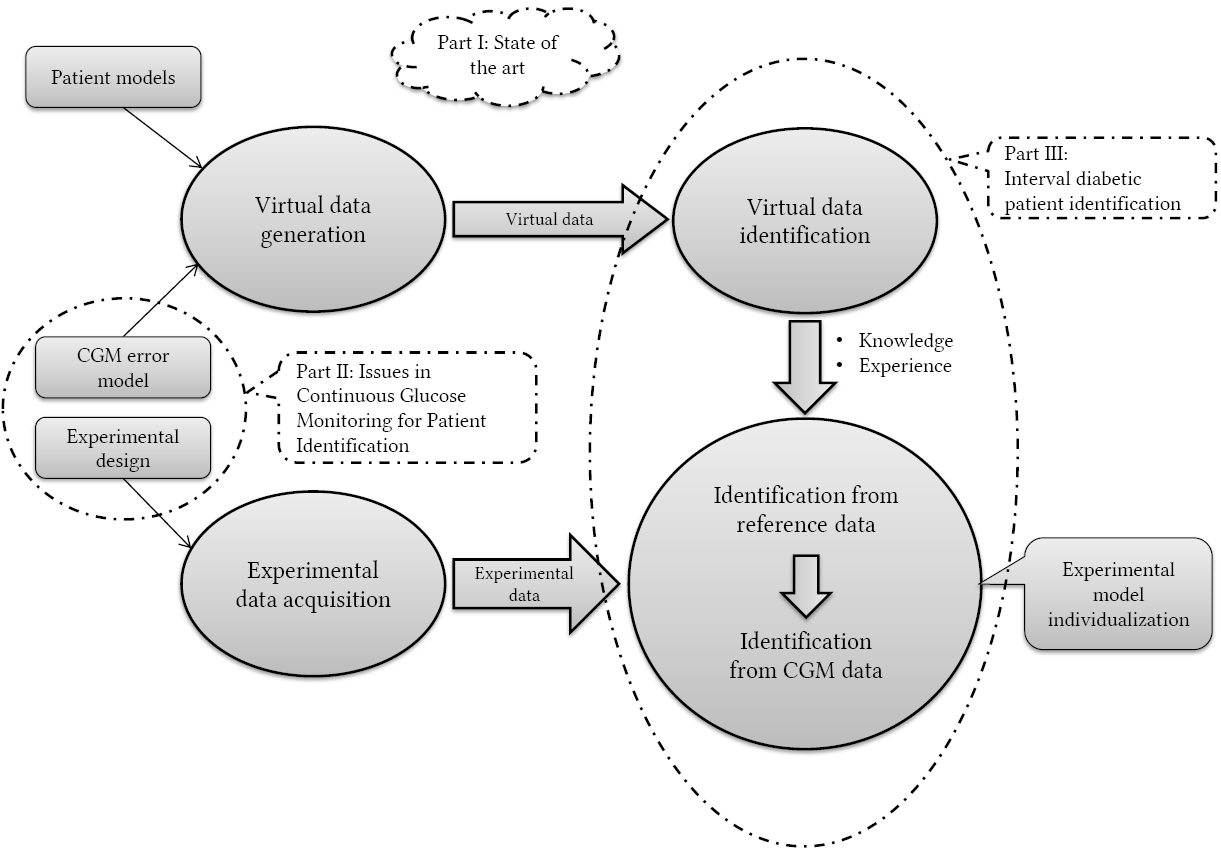
\epsfig{file=Figures/tesis_outline.png, width=\textwidth}\caption{Work-flow schematics for this thesis. The conceptual blocks that correspond to the subsequent parts of this thesis are highlighted in dashed circles.}
\label{fig:thesis_outline}
\end{figure}

A quick visual outline of this thesis contribution can be seen in Figure \ref{fig:thesis_outline}. In there, two work flows can be seen for the execution of an identification experiment in diabetes. This thesis starts (part I) with a literature review of identification in diabetes and associated methodologies. This part of the thesis applies on the background of the workflow depicted in Figure \ref{fig:thesis_outline}.

The first (top) work flow involves the use of virtual patient data for identification experiments. Virtual patient identification is needed for proving the benefits of the proposed identification methodology. The first scientific contributions of this work are comprised in the second part of this thesis, focusing on the improvement of the conditions of identification for both the identification of virtual patients and in the experimental condition. Experimental design focuses on the second (bottom) work flow in Figure \ref{fig:thesis_outline}. This design is carried out using multiple models in order to obtain rich quality data from the diabetic patients. Diabetic patients hospital data is then gathered and analyzed for CGM error modeling, in order to obtain a much more reliable virtual patient simulation, including daily monitoring using a simulated CGM. 

The last part of this thesis is the core identification study. This study is also composed of two parts, one using computer generated data using the CGM models developed earlier, and other using real experimental data from 12 diabetic patients. The differences between virtual and experimental identifications are clearly exposed throughout the thesis, detailing the difficulties that rise when facing real life patient variability. The focus on variability is also constant in this work, and a new identification methodology considering uncertainty is here extensively stated and validated.

\section*{Publications}
\label{sec:Publications}

\subsubsection*{Journal Articles}
\begin{enumerate}
	\item Rossetti P, Ampudia-Blasco F J, Laguna, A J, Revert A, Veh\'{i} J, Ascaso, J F, Bondia J. Evaluation of a Novel Continuous Glucose Monitoring-Based Method for Mealtime Insulin Dosing -the iBolus- in Subjects with Type 1 Diabetes Using Continuous Subcutaneous Insulin Infusion Therapy: A Randomized Controlled Trial. \textit{Diabetes Technology \& Therapeutics} (2012), 14(11), 1043-1052.
  \item Laguna A J, Rossetti P, Ampudia-Blasco F J, Veh\'{i} J, Bondia J. Postprandial performance of Dexcom\textsuperscript{\textregistered} SEVEN\textsuperscript{\textregistered} PLUS and Medtronic\textsuperscript{\textregistered} Paradigm\textsuperscript{\textregistered} Veo\texttrademark{}: Modeling and statistical analysis, \textit{Biomedical Signal Processing \& Control} (2013), http://dx.doi.org/10.1016/j.bspc.2012.12.003
  \item Laguna A J, Rossetti P, Ampudia-Blasco F J, Veh\'{i} J, Bondia J. Identification of intra-patient variability in the postprandial response of patients with type 1 diabetes, \textit{Biomedical Signal Processing \& Control}(2013), http://dx.doi.org/10.1016/j.bspc.2013.07.003
  \item Laguna A J, Rossetti P, Ampudia-Blasco F J, Veh\'{i} J, Bondia J. Experimental blood glucose interval identification of patients with type 1 diabetes, \textit{Journal of Process Control} (2013), 24(1), 171-181.
\end{enumerate}
There is also a paper in preparation with the contents of chapter \ref{sec:ExperimentalIntervalIdentification}.

\subsubsection*{Conference Articles}
\begin{enumerate}
	\item Laguna A J, Rossetti P, Ampudia-Blasco F J, Veh\'{i} J, Bondia J. (2010, September). Optimal design for individual model identification based on ambulatory continuous glucose monitoring in patients with type 1 diabetes. In 2010, UKACC International Conference on Control (pp. 1-6).
	\item Bondia J, Laguna A J, Rossetti P, Ampudia-Blasco F J, Veh\'{i} J. (2011, August). On the Use of Hard/soft Specifications to Deal with Intra-Patient Variability in Postprandial Glucose Control in Type 1 Diabetes. In IFAC World Congress (Vol. 18, No. 1, pp. 8347-8353).
	\item Laguna A J, Rossetti P, Ampudia-Blasco F J, Veh\'{i} J, Bondia J. (2012, August). Identification of intra-patient variability in the postprandial response of patients with type 1 diabetes. In BMS symposium (50, 1-6).
\end{enumerate}

\subsubsection*{Conference abstracts and posters}
\begin{enumerate}
	\item Laguna A J, Rossetti P, Ampudia-Blasco F J, Veh\'{i} J, Bondia J. (2010, October). Improving Postprandial Model Identification Using Ambulatory Data from Type 1 Diabetic Patients. In the Diabetes Technology Meeting 2010
	\item Laguna A J, Rossetti P, Ampudia-Blasco F J, Veh\'{i} J, Bondia J. (2011, February). Designing Optimal Ambulatory Conditions to Improve Prediction Capabilities of Individual Post-prandial Glucose Models. In the 4th International Conference in Advance Technologies \& Treatments for Diabetes 2011
	\item Rossetti P, Ampudia-Blasco F J, Laguna A J, Revert, A, Veh\'{i}, J, Ascaso, J F, Bondia J. (2011, April). C\'alculo del bolus prandial utilizando monitorizaci\'on continua de la glucosa en pacientes con diabetes mellitus tipo 1 tratados con infusi\'on subcut\'anea continua de insulina. In Congreso Nacional de la SED 2011
	\item Rossetti P, Ampudia-Blasco F J, Laguna A J, Revert, A, Veh\'{i}, J, Ascaso, J F, Bondia J. (2011, June). A novel strategy for non-empirical prandial insulin administration in subjects with type 1 diabetes (T1DM) treated with continuous subcutaneous insulin infusion (CSII). In the 71st scientific sessions of ADA 2011
	\item Laguna A J, Rossetti P, Ampudia-Blasco F J, Veh\'{i} J, Bondia J. (2012, February). Postprandial behavior of Dexcom\textsuperscript{\textregistered} SEVEN\textsuperscript{\textregistered} PLUS continuous glucose monitoring system: Statistical analysis and simulation. In the 5th International Conference in Advance Technologies \& Treatments for Diabetes 2012
	\item Rossetti P, Ampudia-Blasco F J, Laguna A J, Revert, A, Veh\'{i}, J, Ascaso, J F, Bondia J. (2012, June). Intra-Subject Variability Makes Prediction of Post-Prandial Glucose Response Difficult in Subjects with Type 1 Diabetes. In the 72nd scientific sessions of ADA 2012
	\item Laguna A J, Rossetti P, Ampudia-Blasco F J, Veh\'{i} J, Bondia J. (2013, February) Uncertainty characterization for the artificial pancreas using interval identification in patients with type 1 diabetes. In the 6th International Conference in Advance Technologies \& Treatments for Diabetes 2013
	\item Laguna A J, Rossetti P, Ampudia-Blasco F J, Veh\'{i} J, Bondia J. (2014, Accepted) Identification of variability in postprandial behavior of patients with type 1 diabetes from insulin pump data. In the 7th International Conference in Advance Technologies \& Treatments for Diabetes 2014
\end{enumerate}


 





 %renombrar a motivation y objetivos. Hablar de la diabetes en el mundo y la individualizacion de pacientes
		
		\part{State of the art}
		\label{sec:stateOfTheArt}
		
		\chapter{Parameter Estimation}
\label{sec:Parameter estimation}

Identification of a model's parameters is an inverse problem. As such, identification consists in the characterization of the inputs and parameters of a system given the outputs and rest of the inputs of such system. Frequently, \textit{a priori} information on the system can be used to narrow the search path of the problem, but this type of information is not enough to allow for a complete derivation of the models. In the glucose-insulin model identification paradigm, the inverse problem is usually reduced to finding the parameters of a model which characterize an individual given the glucose profile of that patient, and the patients information such as meal characteristics and insulin treatments.

\section{Optimization and Intervals}
\label{sec:OptimizationAndIntervals}

Parameter estimation is usually posed as an optimization problem. Its solution relies on optimization algorithms attempting to optimize an index of the fit of the model's output to the available data. Usually scalar indexes are considered for characterizing the deviation of the model from the data. Such indexes can be formulated, for example, as a quadratic error depending on a set of parameters $p$ that has to be minimized:

\begin{equation}
	J(p)=\sum_{i=1}^{N}(y_{i}(p)-\tilde{y}_{i})^{T}Q_{i}(y_{i}(p)-\tilde{y}_{i})
\label{eq:quadraticindex}
\end{equation}

where $y_{i}(p)$ are the model predictions for time $i$ and $\tilde{y}_{i}$ are the experimental measurements, therefore, the data to be fitted. $Q_{i}$ is the data weighting matrix, which permits to fit more accurately some data in detriment to other data samples.  $Q_{i}$ is usually chosen as a diagonal matrix, due to the assumption that data samples are independently correlated to each other. The choice of the diagonal values in the matrix are usually referred to as ``weights'' of the data samples. This quadratic error index reflects the most classical approach to parameter estimation.

A usual compromise choice for the weighting matrix is to make the relative errors of each data sample weight the same in the cost index in order to fit all data points equally in the time axis. This is achieved by forcing the diagonal of $Q_{i}$ to be equal to $1/\tilde{y}_{i}^{2}$. This type of ponderation matrix has the disadvantage of underestimating large errors in high glucose values (hyperglycemic region) of the output of the model than in low values (hypoglycemic case). Usually it is preferred that all errors are normalized in the optimization index, and this is achieved with a different weighting matrix, like for example the case where all the elements of the diagonal are equal to $1/max(\tilde{y}_{i})^{2}$. This way the contribution of every data sample is standardized in the glucose concentration axis.

The most common choice of optimization methods for parameter estimation are simple local optimization algorithms, with iterative executions for easier convergence. There are many drawbacks to the use of local optimization:

\begin{enumerate}
	\item The initial value of the parameters to be chosen for the identification heavily influences the final outcome of the optimization. The choice of these values relies strongly in guesswork.
	\item Convergence to the global optimum of the problem is achievable, but not guaranteed.
	\item There may be several sets of parameters that yield similar optimization index values. This problem may happen with a very flat solution region but it can also happen for different local ``valleys'' of the index function.
\end{enumerate}

These problems are very much present for every model shown in Chapter \ref{sec:ModelsForDiabetes}, and every diabetes model in literature whatsoever. The solution of the identification problem in diabetes has to be focused in the practical aspect of the optimization. It is established in the scientific community that models of the glucose system, even though are often based on physiological aspects of the glucose metabolism, are far away from being accurate. The approach to patient identification is much more focused in the efficacy of the predictions of the model rather than interpretation of the identified parameters. It is then fine for an identification in the diabetes paradigm to achieve a flat solution in the parameter space, if that solution is a global optimum. It is not acceptable though falling on local optimum values of the index, which are likely to provide worst predictions than a global solution. Also, searching for a single optimal value of the parameters set is often not the best option, since there may be a full set of acceptable solutions that fall under feasibility conditions. The use of global search optimization methods is encouraged for this kind of problems.

Identification feasibility or identifiability of a model is the property that determines whether the model is suitable to characterize a set of data and in which terms. Identifiability analysis must be performed prior to any identification study to discard possible incongruences of the model's structure or incompatibilities with the data. Improving identifiability of the models proposed is one of the goals of this thesis, and optimal experiment design will be introduced as one of the main aid tools for diabetic patient identification.

Given that the endogenous glucose system is subject to great parametric variations, uncertainty on the parameter estimation has to be assessed. In local classical methods, uncertainty on the estimate is evaluated (if at all) by using asymptotic properties of the estimator that rely on a number of doubtful assumptions, like assumption of linearity of the parameter's space. This type of uncertainty measurements is not reliable for the diabetes environment and models which are subject to physiologically induced non-linearities both in the input and in the parameter space, and the use of new estimation methods that naturally take uncertainty into consideration is at its utmost importance. Also, intra-patient variability in the diabetic person is a great deal in the parameter estimation, and further encourages the use of some methodology for uncertainty consideration.

A possibility for considering the uncertainty in the parametric space is using interval analysis. Interval analysis has been a very active field in scientific computation for the last 40 years (see for example \cite{moore1979methods}). Intervals are defined as a new kind of numbers, on which all classic arithmetic operations can be performed. An interval $[x]$ is defined as a closed, bounded and connected set of numbers:

\begin{equation}
  \left[ x \right] = \left[ x^{-},x^{+} \right] = \left\{ x \: | \: x^{-}\leq x \leq x^{+}\right\}
\label{eq:intervaldef}
\end{equation}

$x^{-}$ (lower) and $x^{+}$ (upper) are the limits or boundaries of the interval, and are the scalar magnitudes that define it. Another scalar characteristic of the interval that is derived for the boundaries and will be of special interest is its width $w\left(\left[x\right]\right)$, and it is defined as follows:

\begin{equation}
   w\left(\left[x\right]\right)= x^{+}-x^{-}
\label{eq:intervalwidth}
\end{equation}

Interval analysis do not impose any restriction on the internal possible values of the interval further than continuity. This feature makes interval computation very suited to work with uncertain magnitudes naturally by identifying not only scalar values of the model's parameters, but also interval magnitudes of those parameters. Identifying interval parameters allows for the characterization of many sources of uncertainty:

\begin{itemize}
	\item \textit{Parametric uncertainty}. Parameter feasibility vicinity is directly identified by using intervals and no further assumptions are needed.
	\item \textit{Model mismatches}. Unmodelled dynamics can be (artificially) included as larger intervals in the interval identification.
	\item \textit{Measurement errors}. Sensor-induced uncertainty is common in the diabetes paradigm, especially in continuous monitoring systems. Interval identification can be used for consideration of this error (assuming some knowledge on the measurement error) in the identification algorithm.
	\item \textit{Parameter variability}. Parameters that are traditionally considered in model as scalar values can in fact be variant in time, and as such are suited to be identified with uncertainty in interval quantities.
\end{itemize}

Interval parameters in glucose metabolism models produce interval glucose outputs. The power of using interval analysis for simulation relies in the fact that glucose envelopes of an interval model will bound all possible \textit{scalar} simulations of the (scalar) parameters within the bounds of the interval parameters used. This guaranteed outcome of an interval model is true not only for simulations of single parameters, but also for any combination of parameters included in the intervalization of the model. In Figure \ref{fig:intervalenvelope}, a simple simulation of a glucose metabolism model is presented, picturing the envelopes in blue. In green a thousand simulations of the scalar model are plotted where the uncertain parameter is randomly generated within the boundaries of the interval parameter. As can be clearly observed, every possible solution of the original model is contained within the envelopes of the interval model, as expected.

\begin{figure}[hbtp]
\centering
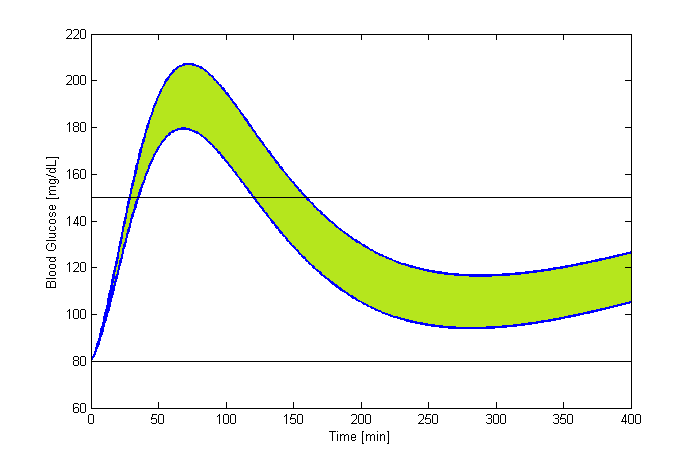
\epsfig{file=Figures/interval.png, width=\textwidth}\caption{Envelopes obtained for an interval simulation of a postprandial period. The simulation considers a 10\% uncertainty in the meal size. The interval bounds are plotted in blue, and the scalar simulations are drawn in green.}
\label{fig:intervalenvelope}
\end{figure}

Intervalization of a given scalar-based model is not straightforward. The computation of both envelopes has to be taken in consideration and depending on the nature of the parameters considered uncertain, the calculations involved can be very complex. Fortunately, interval counterparts of every model proposed in Chapter \ref{sec:ModelsForDiabetes} can be found in literature. In this thesis the intervalization of glucose models will not be reviewed, and instead, it will be taken as given. An extensive review of the models proposed in here was performed by Maria Garcia-Jaramillo in her PhD thesis \cite{mairathesis}, including the intervalization process of every equation and the final interval system of equations of every model. More recently, the model simulated in Figure \ref{fig:intervalenvelope} (model will be reviewed in detail in later chapters) was further improved in its interval form by de Pereda \textit{et al.} \cite{de2012prediction}, including the possibility of simulating as intervals more parameters than the interval version presented by Garcia-Jaramillo. Both versions of the model will be mentioned in the present thesis.

In the rest of this chapter, optimal experiment design and identifiability improvement will be reviewed. Then the interval identification process will be described, including a review of the most used identification algorithms in literature. Finally the optimization tools and software in this thesis will be quickly stated.

\section{Optimizing Identifiability}
\label{sec:Optimizationofidentifiability}

Identifiability analysis can be divided into two stages \cite{walter1997}: \textit{A priori} identifiability and \textit{A posteriori} identifiability. \textit{A priori} identifiability is the feasibility of identification of the model's parameters considering that infinite noise-free data is available. It is an structural property of the model and the lack of it represents a model that can produce the same output with several sets of parameters given a determined input. \textit{A posteriori} identifiability incorporates the data into the identifiability analysis. It analyzes the influence of data noise and uncertainty in the estimation of parameters, and its main outcome is the reliability of an identification.

\subsection{Methods based on FIM}
\label{sec:MethodsBasedOnFIM}

\textit{A posteriori} identifiability often relies in the analysis of the model's parameters sensitivities to the output variations. In the following, the classic method based on the Fisher Information Matrix will be reviewed. Analyzing with detail the Fisher Information Matrix (FIM), all information about \emph{local} identifiability of the model can be extracted, since it implies linearization of the model.

To understand the method, let us take the index defined in equation \eqref{eq:quadraticindex}. The statistical expectation of the index for a set of parameters slightly different than the optimal is given by:

\begin{equation}
	E[J(p+\delta p)]\cong \delta p^{T}\left[\sum_{i=1}^{N}{(\frac{\partial z}{\partial p}(t_{i}))^{T}Q_{i}(\frac{\partial z}{\partial p}(t_{i}))}\right]\delta p + \sum_{i=1}^{N}{tr(V_{i}Q_{i})}
\label{eq:indexdiff}
\end{equation}

where $V_{i}$ represents the covariance matrix of the measurement errors ($Q_{i}$ is typically chosen as $V_{i}^{-1}$), $z$ is the model output and $N$ is the number of data samples. The term between brackets is the Fisher Information Matrix and it expresses the quantity of information contained in the experimental data, as explained in detail by Ljung \cite{ljung1999system}:

\begin{equation}
	FIM=\sum_{i=1}^{N}{\left(\frac{\partial z}{\partial p}(t_{i})\right)^{T}Q_{i}\left(\frac{\partial z}{\partial p}(t_{i})\right)}.
\label{eq:FIM}
\end{equation}

The terms $\partial z /\partial p$ are the sensitivity functions of each parameter $p$ and they are of great importance for the evaluation of the practical identifiability since they gather the parameter influence on the output of the system. The FIM is a square matrix with dimension equal to the number of parameters that are to be identified. The inverse of the FIM is an approximation of the covariance matrix of the estimation error of the model parameters:

\begin{equation}
	C=FIM^{-1}=\left[\sum_{i=1}^{N}{(\frac{\partial z}{\partial p}(t_{i}))^{T}Q_{i}(\frac{\partial z}{\partial p}(t_{i}))}\right]^{-1}
\label{eq:BLUE}
\end{equation}

The diagonal of $C$ contains the information of the confidence interval in the estimation of every parameter. The statistical expected value of the error of an estimation (which is a measure of the confidence interval of the model's parameters) is actually bounded by the matrix $C$ following the Cramer-Rao inequality for unbiased estimators (the true value of the parameters equals the expectation of the estimated parameters), as introduced originally in the classic references \cite{cramer1946mathematical} and \cite{rao2009linear}. 

\begin{equation}
	E \left( \left[ \hat{p}-p\right]\left[ \hat{p}-p\right]^{T}\right) \geq C
\label{eq:CRineq}
\end{equation}

where $E$ stands for the statistical expected value and $\hat{p}$ is a estimation of the parameters $p$. For further explanations and proofs of the Cramer-Rao inequality, the reader is referred to Ljung's work \cite{ljung1999system}. Given that the FIM is known and that it is invertible (non-invertability means structural non-identifiability), the coefficient of variation (CV) for the parameter $p_{i}$ being identified is calculated as:

\begin{equation}
	CV_{i}=\frac{\sqrt{C_{ii}}}{p_{i}}
\label{eq:CR}
\end{equation}

The interpretation of this confidence interval limit is simple: if, for example, a parameter $p_{i}$ has a CV of $0.4$ it means that, for the measurement error which variance was considered in the calculation of $Q_{i}$, successive parameter estimations will have a standard deviation of 40\% of the true parameter value (for a fully efficient unbiased estimator). There is more useful information to be drawn off the FIM, like the correlation matrix. This matrix, the elements of which are the approximated coefficients of correlation between the $i^{th}$ and the $j^{th}$ parameters, is defined as:

\begin{equation}
	R_{ij}=\frac{C_{ij}}{\sqrt{C_{ii}C_{jj}}}
\label{eq:FIMcorrelation}
\end{equation}

Analyzing the correlation matrix gives information on the compensation effect of the changes in the values of the parameters over the model output. If two parameters, $p_{i}$ and $p_{j}$, are highly correlated, a change in the output due to a change in parameter $p_{i}$ can be hidden by the appropriate change in $p_{j}$. Very strong correlations between different parameters are a display of poor identifiability of a model. A correlation of value 1 between parameters is a sign of a structural problem of identifiability of the model, because both parameters have the same exact effect on the model's output. Thus, FIM analysis can also be used in the process of \textit{a priori} identifiability analysis by identifying structural identifiability problems.

\subsection{Monte-Carlo methods}
\label{sec:MonteCarloMethods}

Calculation of the coefficients of variation and the confidence region of the parameters in an identification using the FIM is an approximation of the ``real'' confidence in the parameter's identification. Further methods are explored in literature to obtain better approximations of the CV without incurring in too many approximations. The group of methods for parameter uncertainty estimation that make less assumptions on the parameters distribution is the group of Monte-Carlo methods.

Parameter estimation using data collected from a system will generally not yield the same results if the experiment is repeated, because of the perturbations acting on the system and noise in the measurement systems. The vector of outputs of the system is then a random vector $y^s$ that is related to an estimation of the parameters $\hat{p}(y^s)$. Monte-Carlo methods aim to estimate $\hat{p}(y^s)$ and its confidence region by creating a set of fictitious data vectors with a mathematical model and incorporating realizations of random variables in order to simulate the influence of noise and perturbations, creating the \emph{virtual dataset} $y^m$. Several realization runs of the model applied to different realizations of the ``noise'' will create different estimations $\hat{p}(y^m)$ of the parameter vector.

One of the difficulties of the Monte-Carlo methods lies in the choice of the distribution used to generate the fictitious data $y^m$. The \textit{jack-knife} \cite{quenouille1949approximate} and the \emph{bootstrap} \cite{efron1982jackknife} methods make it possible to avoid estimating the distribution of the noise from the residuals.

\subsubsection{Jack-knife}
\label{sec:JackKnife}

The main advantage of this approach is its simplicity. The virtual data is fragmented in $n_t$ vectors of equal size $y^m_i, (i=1, \ldots , n_t)$. Let $\hat{p}$ be the estimate of the parameters obtained from all the virtual data vector, and $\hat{p}_i$ the estimator related to all the data but $y^m_i$. Then $n_t$ pseudo-estimates can be defined as

\begin{equation}
	\tilde{p}_i=n_t \hat{p} - (n_t -1) \hat{p}_i \quad (i=1, \ldots , n_t)
\label{eq:jackknifepseudo}
\end{equation}

And the computation of the average of these pseudo-estimates is the jack-knife estimator of $\hat{p}(y^s)$, denoted as $p_{jk}$. The covariance matrix of the population of pseudo-estimators $\tilde{p}_i$ is

\begin{equation}
	C_{jk}= \frac{1}{G-1}\sum_{i=1}^{n_t} (\tilde{p}_i-p_{jk})(\tilde{p}_i-p_{jk})^T
\label{eq:jackknifecovariance}
\end{equation}

And the $100(1-\alpha)\%$ confidence interval for a given $p_i$ parameter can be calculated using the $T^2$ Hotelling distribution:

\begin{equation}
	p_{jk_i}\pm t^{1-(\alpha/2)}_{N-N_p}\sqrt{\frac{C_{jk_{ii}}}{n_t}}
\label{eq:jackknifeconfidence}
\end{equation}

where $C_{jk_{ii}}$ are diagonal elements of $C_{jk}$ and $p_{jk_i}$ is the $i$\textsuperscript{th} element of $p_{jk}$.

\subsubsection{Bootstrap}
\label{sec:Bootstrap}

This approach assumes that the errors are independent random variables with identical but otherwise unspecified distribution. In order to obtain an estimation of the parameters $\tilde{p}$, this method uses only the experimental values $y^s$ and the model simulated output values $y^m$. Let us assume

\begin{equation}
	y^s(t_i)=y^m(t_i,p^{*})+b_i \quad (i=1, \ldots , n_t)
\label{eq:bootstrapy}
\end{equation}

where $p^{*}$ is the real value of the parameter vector, and $b_i$ correspond to independent random variables with the same distribution. Then, an estimate of $b_i$ is given by the $i$\textsuperscript{th} residual:

\begin{equation}
	\hat{b}_i = y^s(t_i)-y^m(t_i,\hat{p}) \quad (i=1, \ldots , n_t)
\label{eq:bootstrapbi}
\end{equation}

where $\hat{p}$ is the estimate of the vector $p*$. A vector of virtual data $y^f$ is then obtained as

\begin{equation}
	y^f(t_i)=y^m(t_i,\hat{p})+\hat{b} \quad (i=1, \ldots , n_t)
\label{eq:bootstrapyf}
\end{equation}

where $\hat{b}$ is chosen among the residuals $\hat{b}_k; \; (k=1, \ldots , n_t)$ for every $t_i$ with equal probability for every $\hat{b}_k$. This is equivalent to substituting the empirical distribution of residual for the true distribution of the $b_i$'s, which is more acceptable the closer $\hat{p}$ is to $p*$. Repeating this operation for different runs of the model, a population of fictional vectors of data can be obtained, and similarly to the jack-knife approach, the mean of the population ($p_B$) and the covariance matrix ($C_B)$ can be used to deduce a $100(1-\alpha)\%$ confidence interval for the parameter $p_i$ as follows:

\begin{equation}
	p_{B_i}\pm t^{1-(\alpha/2)}_{N-N_p}\sqrt{C_{B_{ii}}}
\label{eq:bootstrapconfidence}
\end{equation}

where $C_{B_{ii}}$ are diagonal elements of $C_{B}$ and $p_{B_i}$ is the $i$\textsuperscript{th} element of $p_{B}$.

\subsection{Practical Identifiability and Optimality}
\label{sec:PracticalIdentifiability}

Monte-Carlo methods for uncertainty estimation can be too cost effective for large datasets and models, such as those present in the work developed in this thesis. Therefore, FIM based methods for identifiability calculation are used in this thesis from this point onward.

In practical terms, the identifiability analysis must be done applying some simplifications. The sensitivities of the parameters have to be calculated by approximating the derivatives of the output with first order approximations. In general, application of the analytic expression of the derivative function is the correct way of performing the FIM calculation. Regarding the models of diabetes in literature though, the analytical expression of the derivative with respect to the parameters of the model's output is not feasible.

Usually, the sensitivity function is calculated by linearizing the model around the nominal parameter, and obtaining the symmetric first order difference. In practice, two simulations of the model are calculated, one with a positive variation of the selected parameter, and the other with a negative variation and then the sensitivity function, resulting in practice in a linearization of the derivative. The sensitivity function is computed using equation \eqref{eq:Slinearization}.

\begin{equation}
	S_{p}=\frac{z(p+\Delta p)-z(p-\Delta p)}{2\cdot \Delta p}
\label{eq:Slinearization}
\end{equation}

Also, if the FIM results to be singular it can not be inverted, and that is considered a sign of non-identifiability. In fact, it is a sign of \textit{a priori} non-identifiability, so \textit{a priori} identifiability analysis is being carried out with this method as well. Usually, when working with noisy measurements, it is really difficult to get a singular FIM, and yet it will be difficult to identify any parameter because the FIM is bad-conditioned. The condition number of the FIM has to be analyzed to overcome this computation problem, and its magnitude checked to analyze if it permits inversion of the matrix and therefore identifiability of the model.

Identifiability of a model depends on model structure, and the data used for identification. Identifiability of a model can be improved by conditioning the data used for identification, and designing optimal experiments for the model used. So far, identifiability has been analyzed as a property of a parameter, quantified as the confidence interval in the estimation of each parameter. That information is obtained from the Fisher Information Matrix (or better, from its inverse), which summarizes the information of all the parameters of the model for a given experiment. The problem of optimal experiment design can be expressed then as an optimization problem of finding the minimum value of a certain scalar function of the FIM that optimizes the identifiability of the model. That scalar function is called optimality criteria, and its general expression is:
\begin{equation}
	j(\Xi)=\phi[FIM(p, \Xi)] \\
\label{eq:index}
\end{equation}
where $\phi$ is a scalar function. The evaluation of the Fisher Information Matrix is a function $FIM$ of $p$, the parameters vector, and $\Xi$, the experiment conditions to be optimized.

There are several criteria that can be used in this case, as seen in \cite{franceschini2008model}:
\begin{itemize}
	\item D-optimality, in which the scalar function chosen is the determinant of the FIM. The three following equations are equivalent, and all of them define the D-optimality criterion and whether it has to be maximized or minimized in order to improve identifiability:
	\begin{align}
		\Xi &= argmin_{\Xi} \: det(FIM^{-1}(p, \Xi)) \label{eq:Doptimality1} \\
		\Xi &= argmax_{\Xi} \: det(FIM(p, \Xi)) \label{eq:Doptimality2} \\
	  \Xi &= argmax_{\Xi} \: ln(det(FIM(p, \Xi)) \label{eq:Doptimality3}
	\end{align}
	\item E-optimality, in which the function is the smallest eigenvalue of the information matrix, and it has to be maximized.
	\item A-optimality, in which the problem is solved by maximizing the trace of the information matrix.
\end{itemize}
In order to better understand the meaning of these criteria a geometrical analogy is needed. If every parameter is placed in an axis of the geometrical space, then the region defined by the confidence intervals of each one of the parameters defines an ellipsoid the axis of which are given by the eigenvalues of the inverse of the information matrix. Given that the objective of the optimization is to minimize all the regions of confidence, every axis of the ellipsoid have to be minimized, or equivalently, the volume of the ellipsoid has to be minimized, and that volume is exactly the determinant of the inverse of the FIM. The rest of the criteria have similar meanings that are summarized in Figure \ref{fig:criteria}.

\begin{figure}[hbtp]
\centering
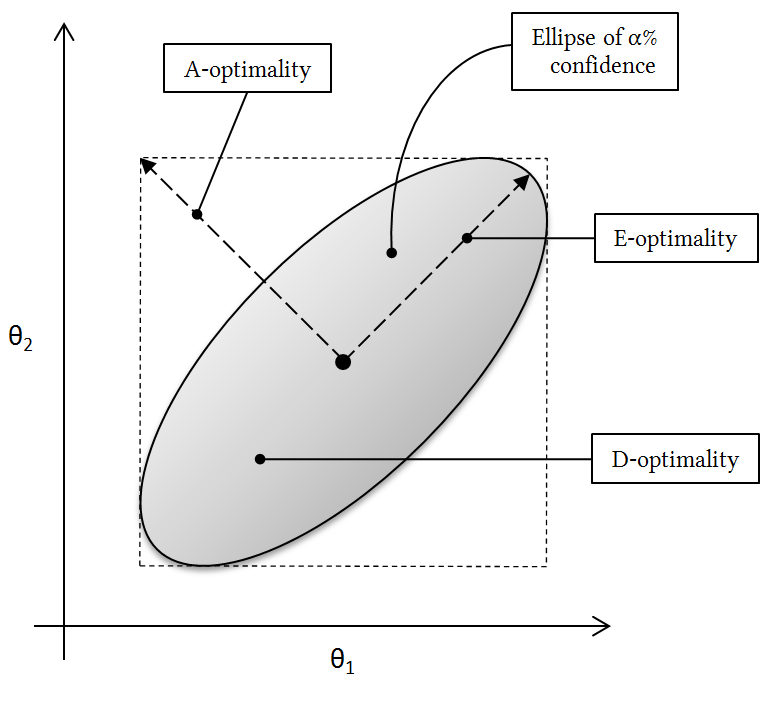
\epsfig{file=Figures/optimalcriterion.png, width=0.7\textwidth}\caption{Each criterion reduces the confidences intervals attempting to minimize one singular scalar value. Adapted from \cite{franceschini2008model}.}
\label{fig:criteria}
\end{figure}

The question of which criterion should be used arises now. The D-optimality is the most used of the three standard criteria cited above. This is due to some exclusive appealing properties of the criterion \cite{franceschini2008model}:
\begin{itemize}
	\item Easy geometrical interpretation, as seen in Figure \ref{fig:criteria}.
	\item Invariance with respect to non-degenerated transformation applied to the model parameters, such as rescaling. This property is applied in equation \ref{eq:Doptimality3} in order to work, during the optimization process, with smaller quantities.
	\item Yielding to optimal experiments which correspond to replications of a small number of different experimental conditions.
	\item Optimal experiment design yields to non-singular FIM.
\end{itemize}
The main drawback this criterion has is that it gives too much importance to the parameter to which the model is most sensitive. Geometrically, this problem is equivalent to the idea of trying to minimize the volume of the ellipsoid by reducing mostly its bigger axis.

There are other criteria available for different purposes, like the modified E-optimality, that tries to maximize the FIM condition number, aiming to make the confidence ellipsoid as spherical as possible \cite{versyck1998optimal}. The correct application of this criterion would be in a case of strong parameter correlations, and the design will yield to a decoupled identification in parameters. That is not the case in this thesis though. D-optimality will be the one used for the experiments designed for diabetic patients, and for every model tested.

The optimization problem associated is non-linear, and global solvers are suggested for its solution. The choice of experimental parameters for the optimization is as wide the experimentation ambit. One of the most common choices is to optimize the sampling times of a given experiment. The choice of these parameters usually relies on the person performing of the experiment design, but it conditions the characteristics of the optimization. Too many parameters may lead to long, unrealistic convergence times on the optimization algorithm, or even non convergence at all. Also, if many experimental parameters are introduced experimental setup may be too complicated to perform. Given this arguments, and especially in the diabetes context, the number of parameters to be optimized should remain as low as possible for achieving the maximum identifiability needed.

\section{Identification with Uncertainty}
\label{sec:IntervalIdentification}

The use of intervals for identification has been developed since the 1990s due to its ability to cope with uncertainty either in the structure of the model and also in the measurements and parameters. Focusing on the measurement error, a parameter estimation methodology outstands over all others: the error-bounded estimation.


\subsection{Error-bounded Estimation}
\label{sec:ErrorBoundedEstimation}

Error bounded estimation assumes that an error exists in the measured variable, and that there exist a trusted estimation of this error. The estimated error must be within bounds that are acceptable for the good working of the system. One may define the error as:
\begin{equation}
	e(p)=\tilde{y}-y(p)
\label{eq:output_error}
\end{equation}
where $\tilde{y}$ is the vector of experimental measurements, and $y(p)$ is the model output, which is dependent on the parameter vector $p$. The problem of bounded error estimation considers that the output errors lie within acceptable bounds:
\begin{equation}
	e^{-} \leq e(p) \leq e^{+}
\label{eq:error_bound}
\end{equation}
where $e^{-}$ and $e^{+}$ are the lower and upper acceptable bounds of the error. The identification problem relies on finding all possible values of the parameter vector $p$ that produce outputs that fall within the acceptable bounds. The subsequent problem is a set inversion problem, and it can be solved by set inversion algorithms like the SIVIA (Set Inversion Via Interval Analysis) algorithm presented in Jaulin \textit{et al.} \cite{jaulin2001applied}.

The SIVIA algorithm divides the parameter space into ``boxes'', i.e multidimensional intervals, and evaluates the correspondent image in the output space for compliance with the desired characteristics. Given that interval analysis produces guaranteed solutions of the output of the model to all the values of the parameter space inside the evaluated box, classification of the boxes evaluated can be divided into three categories:
\begin{itemize}
	\item Guaranteed solutions. All parameters in the evaluated box lead to an output error fulfilling the constraints.
	\item Guaranteed non-solutions. All parameters in the evaluated box lead to an output error violating the constraints.
	\item Indeterminate solutions. Otherwise.
\end{itemize}
The algorithm works iteratively classifying the boxes into these three categories and dividing indeterminate boxes into smaller boxes for further classification. The algorithm searches all the parameter space. The accuracy of the algorithm is given by the acceptable size of the indeterminate boxes in the parameters space. These boxes compose the boundary of the parameter space that produces outcomes of the model in the acceptability constraints.
\begin{figure}[hbtp]
\centering
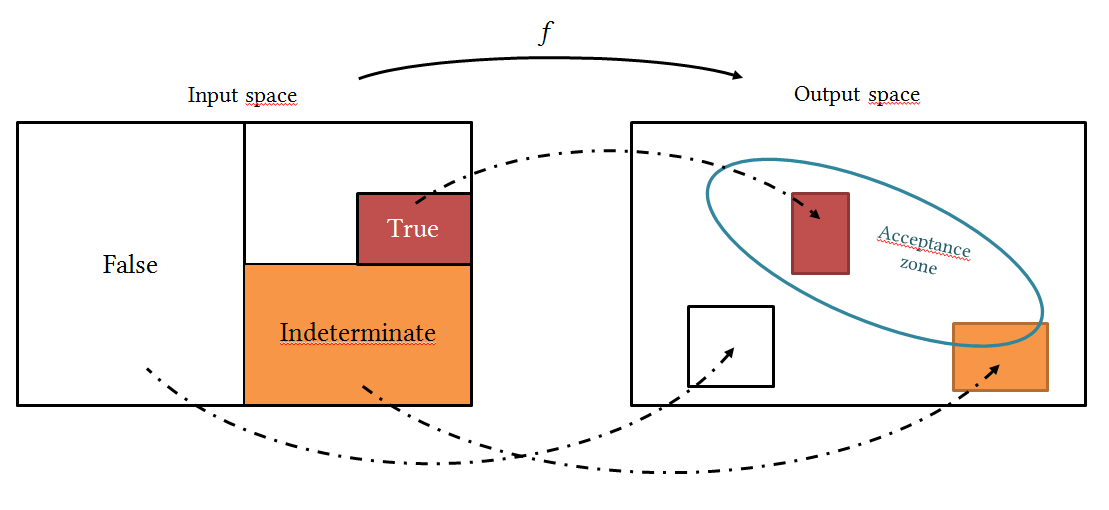
\epsfig{file=Figures/sivia.png, width=\textwidth}\caption{Basics of the SIVIA algorithm. The boxes that produce images in the output space that fall within the acceptability range (red ellipse) are classified as true solutions, in blue. Boxes out of the acceptability zone are classified are false solutions and marked in white. Red boxes are undetermined. Adapted from \cite{jorgeibolus}}
\label{fig:sivia}
\end{figure}
The SIVIA methodology is summarized in Figure \ref{fig:sivia}. The images in the output space are related to boxes in the input (or parameter) space. The boxes in the input space are divided each time they are classified as undetermined. The first evaluation to be performed correspond to the whole parameter space, which will be evaluated as undetermined if the acceptability criterion embraces only some part of the output space. The parameter space is then divided using a predefined criterion to the choice of the user into smaller boxes, and reevaluated. The algorithm then works as a tree-search algorithm, finishing a branch when it is classified into true or false solutions, or if the resolution threshold for the search boxes is met.
%A classic example of the performance of error-bounded estimation will be reproduced next in order to better display this set inversion problem. A simple two parameter model is to be fit to data with consideration of uncertainty in it. The data for the example was first found in \cite{milanese1991estimation}. The model to be fit responds to the equation:
%\begin{equation}
%	y(p_{1},p_{2},t_{i})=20 \exp(-p_{1} \, t_{i})-8 \exp(-p_{2} \, t_{i})
%\label{eq:error_bound_ex}
%\end{equation}
%where $p_1$ and $p_2$ are the parameters to be identified with uncertainty. The data for the identification was sampled at different times, and it presented different relative error known \textit{a priori} following $[e]=[-e_{max},e_{max}]$ with $e_{max}=0.5\left|\tilde{y}\right|+1$, where $[e]$ is the vector of acceptable intervals for the error and $\tilde{y}$ are the experimental measurements. Notice that the error estimation is considered as given for the problem. The vector of sampling times and related experimental measurements with the error interval associated to each sample are displayed in Table \ref{tab:error_bounded_example}. The same samples are displayed in Figure \ref{fig:error_bounded} in a Cartesian plot for easier visualization of the problem.
%\begin{table}[hbtp]
%	\centering
%		\begin{tabular}{|c c c|}
%		\hline 
%		$i$ & $t_{i}$ & $\tilde{y}$ \\
%		\hline 
%		$1$ & $0.7$ & $[2.7, 12.1]$ \\
%	  $2$ & $1.5$ & $[1.04, 7.14]$ \\
%		$3$ & $2.25$ & $[-0.13, 3.61]$ \\
%		$4$ & $3$ & $[-0.95, 1.15]$ \\
%		$5$ & $6$ & $[-4.85, -0.29]$ \\
%		$6$ & $9$ & $[-5.06, -0.36]$ \\
%		$7$ & $13$ & $[-4.1, -0.04]$ \\
%		$8$ & $17$ & $[-3.16, 0.3]$ \\
%		$9$ & $21$ & $[-2.5, 0.51]$ \\
%		$10$ & $25$ & $[-2, 0.67]$ \\		
%		\hline 
%		\end{tabular}
%	\caption{Measurement times and corresponding interval data.}
%	\label{tab:error_bounded_example}
%\end{table}
%\begin{figure}[hbtp]
%\centering
%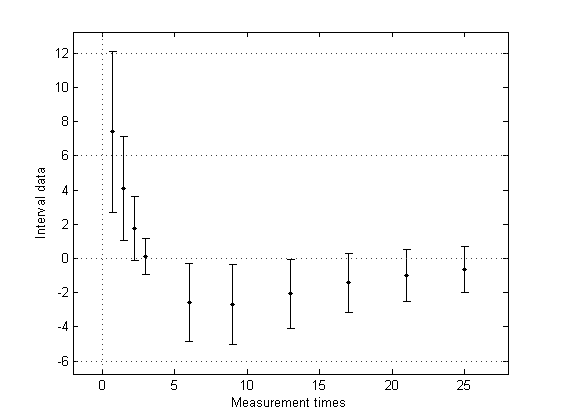
\epsfig{file=Figures/errorbounded.png, width=\textwidth}\caption{Acceptable data measurements including data uncertainty displayed as vertical bars (extracted from \cite{milanese1991estimation}).}
%\label{fig:error_bounded}
%\end{figure}
%The error bounded identification for this data-set is defined as the set of parameters $p_1$ and $p_2$ that create curves from equation \eqref{eq:error_bound_ex} that cross all the vertical bars in Figure \ref{fig:error_bounded}, which represent the experimental values. The set of solutions from the error-bounded identification then represents all possible model outcomes that are compliant with the error estimation considered. The solution set in the parameter space is shown in Figure \ref{fig:error_bounded_solution}. The thinner boxes represent the boundary of the optimization algorithm where the resolution threshold was met. All the boxes within the boundary are guaranteed solutions to the problem, and the boxes out of the boundary are guaranteed not to be solutions.
%\begin{figure}[hbtp]
%\centering
%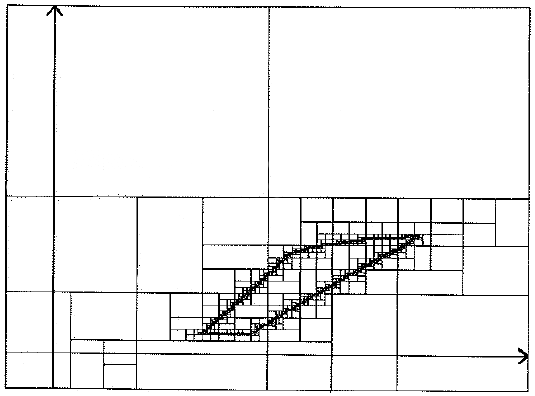
\epsfig{file=Figures/error_bounded_ex_solution.png, width=0.7\textwidth}\caption{Parameter space for the parameters $p_1$ and $p_2$. The frame corresponds to the search domain $[-0.1, 1]^{2}$ (extracted from \cite{jaulin1993guaranteed}).} 
%\label{fig:error_bounded_solution}
%\end{figure}

Even though error-bounded estimation is very extended within the scientific community, it depends heavily on the estimation of the error assumed in the measurements. In the context of diabetes monitoring, errors associated to continuous glucose monitoring are often very large \cite{mazze2009evaluating} which makes CGM estimations too noisy for a closed loop control environment, given the complexity of the models associated. In the hospital environment is possible to obtain much more reliable measurements, with errors smaller than the 2\% \cite{nowotny2012precision}, which can always be neglected for identification. 

Error-bounded estimation is very much focused in the search of feasibility of a group of parameters with the uncertainty of the measurement, although it can also be used for consideration of parametric variability. For control-oriented identification, finding all possible values of the parametric space in which the model's parameters move (system's variability) is more important than finding the feasible parameter set that matches the uncertainty in the measurement. Therefore, a successful robust controller has to respond to system's variability, but never neglecting the influence of measurement errors.

\section{Software and optimization tools}
\label{sec:OptimizationAndSoftware}

Identification and optimization is usually a computationally intensive task. Global non-convex optimization is especially demanding in computation requirements, and it has been established that identification on model identification in diabetes relies on global optimum solutions. There is a wide variety of optimization methods available in literature, but in the following lines we will quickly review the algorithms to be used in this thesis.

All data analysis and computations were done in the Matlab environment, release 2012a (Mathworks, Natick, MA).

\subsection{Scatter search for Matlab}
\label{sec:ScatterSearchForMatlab}

Scatter search for Matlab (SSM from now on) is a global optimizer based on statistical principles and geometrical analysis of the parameter space. This search algorithm has already been used in the artificial pancreas environment with the objective of patient identification, by Cesar Palerm in Santa Barbara \cite{palerm2006robust}.

SSM optimizer is a project of the CSIC (Centro Superior de Investigaciones Cientificas) and the University of Vigo. It is a global optimizer, easily comparable with genetic algorithms. However, SSM does not use codification of the population as genetic algorithms do, although it does work by spawning new generations (offspring) of the function optimum by combining the properties of the previous (parents) population. SSM does not generate random ``mutations'' on the population, as opposed to genetic algorithms, although it renews the existing individuals by adding new random samples to the new generations of optimal solutions in each algorithm iteration. For the details of the inner working of the algorithm, information on the computational cost and better understanding of the searcher the reader can refer to Julio Banga's group papers in 2006 \cite{rodriguez2006novel} and 2007 \cite{egea2007scatter}.

This optimizer has the advantage of using local solvers to refine the search when it seems to have found some optimum solution. The local solver to be used can be chosen from a list available in the SSM's documentation. The local solver chosen was the \textit{fmincon} solver, which is implemented in Matlab's Optimization Toolbox, along with many other optimizers and aid tools for solving any optimization problem in the Matlab environment. This local solver fits into the group of solvers denominated as ``Nonlinear programming solvers'', or ``Constrained nonlinear optimizers''. This sort of algorithms are deterministic solvers that use first and second derivatives of the objective function, along with some heuristics to cope with the various problems that deterministic local searchers have. Abundant information about this kind of algorithms can be found in Coleman and Li paper of 1996 \cite{coleman1993interior}, Powell's conference in 1978 \cite{Powell1978NLSQP}, or for a more general reference see Bazaraa's book \cite{bazaraa2006nonlinear}.

\subsection{Covariance Matrix Adaptive Estimation}
\label{sec:CovarianceMatrixAdaptativeEstimation}

A very well known global optimization method within the scientific community is the algorithm of estimation based on adaptations of the matrix of covariance of the sample population (CMAES). CMAES performs very fast optimizations on a single objective even for large parameters spaces. The optimization performed by CMAES is based on the update of generations of sampling individuals, in a similar way as an evolutionary algorithm, although the update process and the randomly generated individuals are handled differently.

CMAES uses statistical properties of the populations and updates them in each iteration based on the characteristics of the population and the explored parameter space. The adaptation objective in on the covariance matrix adaptation moves the sampling population in order to better fit it to the contour lines of the objective function being minimized. It is assumed that the optimal covariance matrix equals the inverse of the Hessian matrix, although this is only strictly true in convex-quadratic functions. For general optimization functions, the CMAES methodology aims to approximate the inverse of the equivalent of the Hessian matrix for the objective function properties. Convergence and performance of this family of algorithms can be accessed in the proceedings of the 2005 IEEE Congress on Evolutionary Computation \cite{auger2005restart}. For further explanation on the CMAES rational, and its computational analysis, the reader is referred to the works of Hansen in \cite{hansen2006cma} and \cite{hansen2004evaluating}.

Optimizations using interval parameters may consist of two independent parameter sets, upper and lower bounds, where obviously all the lower bounds must be smaller than their respective upper bounds. These greater-or-equal restrictions introduce further constraints on the optimization index. Unfortunately, the build released by Hansen \textit{et al.} \cite{hansen2004evaluating} does not implicitly consider restrictions neither in the outputs nor in the inputs, so they have to be integrated in the cost index with a penalty method.

\subsection{$\epsilon$- MOGA Evolutionary Algorithm}
\label{sec:EpsilonMOGAEvolutionaryAlgorithm}

Classic parametric identification results in a single ``optimal'' point in the parameter space, being insufficient for the case of a time-varying model based on poor prediction capabilities. Many problems in engineering can be translated to multiobjective optimization problem, including the diabetic patient identification problem. In the case of identification in presence of uncertainty using interval models, a problem of optimization of two objectives can be suggested: minimization of glucose interval width and minimization of the fitting error. This problem will be explained in detail in the following thesis, and multiobjective optimization algorithms are used to find it's solution. A brief explanation of these kind of algorithms follows, along with the details of one particular methodology used in this work.

Multiobjective identification is the process of simultaneously optimizing two or more conflicting objectives subject to certain constraints. The solution of this kind of problems is not a single optimal point in the objectives search space, but a family of solutions called a Pareto Front (PF). PF present advantages over single objective optimization techniques:
\begin{itemize}
	\item Provide the designer with the possibility of a better selection of the final solution, presenting a wide variety of possibilities that in many cases include the single objective solution of an analog problem.
	\item Are representative of the whole space of design variables, all of them optimal.
	\item Require of no \emph{tradeoff} parameters to be tuned in the algorithm.
\end{itemize}
PF are created on the basis that each individual in the family is non-dominated by the other individuals. An individual is dominated by other in the population if its evaluation in \emph{both} of the optimization objectives is worse. Therefore, an individual is considered non-dominated and included in the PF by the algorithm if it is best solutions for both objectives in a particular region of the objective space i.e. it cannot be replaced by other point in the objective space for improving an objective, without worsening another one. 

\begin{figure}[hbt]
\centering
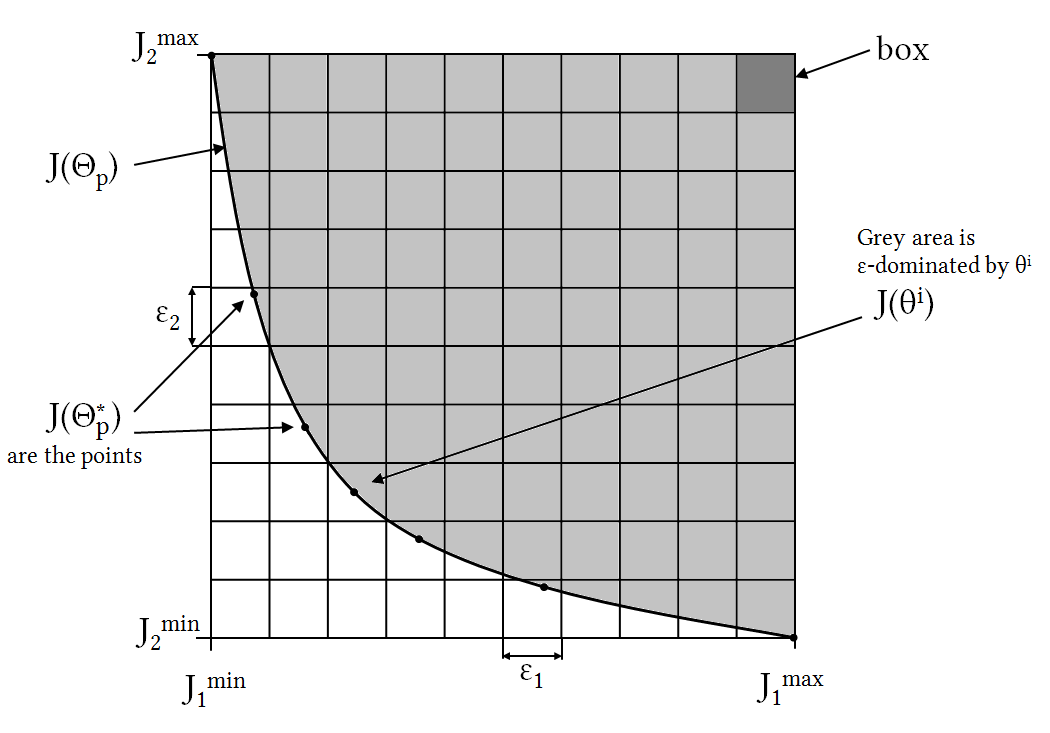
\epsfig{file=Figures/eps_dominance.png, width=0.8\textwidth}\caption{Display of the concept of $\epsilon$-dominance. $J(\Theta_p)$ represents the PF interpolation and $J(\Theta_p^*)$ the actual PF individuals. $J_1$ and $J_2$ are the objective variables, and $\epsilon_1$ and $\epsilon_2$ are the box widths (adapted from \cite{herrero2007well}).}
\label{fig:eps_dominance}
\end{figure}

Evolutionary algorithms are popular solvers for multiobjective problems because of Pareto front groups being susceptible to evolution rules, and both the solver and the problem being population based methods. The $\epsilon$-MOGA (Multi Objective Genetic Algorithm) evolutionary algorithm developed by \cite{herrero2007well} takes the concept of dominance an step further with the notion of $\epsilon$-dominance. $\epsilon$-dominance is based on the domination concept explained before, but it ads a new constraint to the PF individuals: each individual must be isolated within a box of previously defined magnitude. The concept of $\epsilon$-dominance is clearly displayed in Figure \ref{fig:eps_dominance}, where the objective space is overlapping a grid of equally dimensioned boxes. Dominance is then applied to the box in which the Pareto individual is placed, and not just to the point in the objective space. This box-dominance is the $\epsilon$-dominance of the individual of the PF in that box.

The $\epsilon$-MOGA algorithm is able to characterize all kind of PF, including non-convex, non-linear discontinuous search spaces, which is the case for diabetic patient models optimization. The algorithm converges faster than similar evolutionary algorithms, and supposes a smaller computational burden \cite{juanmatesis}. The main achievement of this algorithm is the fact that the PF obtained from $\epsilon$-dominance are well-distributed in the objective space independently of the problem, which is not the case for any other multiobjective optimization algorithm. A well distributed PF is of great help in the interpretation of the results, and can be of utility when choosing an individual out of the PF with a decision making methodology.


 
		
\chapter{Models for the artificial pancreas development}
\label{sec:ModelsForDiabetes}

% Se podria añadir un epigrafe con el quote de box "essentially, all models are wrong, but some are useful" http://en.wikiquote.org/wiki/George_E._P._Box

One of the main problems for glucose control is the insufficient accuracy of existing mathematical models for describing the physiology of the glucoregulatory system. In this chapter the modeling context for the artificial pancreas will be reviewed, and the state of the art of mathematical models in literature will be described.

\section{Introduction}
\label{sec:Introductionfodiabetes}

A mathematical model is characterized both by its objective and its structure. The main objective in modeling a type 1 diabetic subject is of course to be able to reproduce the patient's metabolism from a clinical point of view. In the artificial pancreas context, models must be useful from the control point of view. According to the structure of a model, quoting the work of Walter and Pronzato \cite{walter1997}, the main distinction to be made is whether a \textit{phenomenological} or \textit{behavioral} modeling approach must be followed. A phenomenological model is a model based on prior knowledge about physical or, in the case of the artificial pancreas, physiological principles. This kind of processes are often called \textit{knowledge-based} models as opposed to behavioral models, which merely approximate the observed behavior of the output without any prior knowledge of the process. Behavioral models are focused on data reproduction, and not at all in the process behind, while phenomenological models only use the data to adjust the parameters, while the structure is determined by the process itself.

Examples of phenomenological models are:
\begin{itemize}
	\item Chemical reactions. Biological reactions.
	\item Systems of force equilibrium.
	\item Models of deposit systems.
	\item Electromagnetic models. Electrical engines.
\end{itemize}
Examples of behavioral models are:
\begin{itemize}
	\item ARX/ARMAX models.
	\item Polynomial models.
	\item Random models.
\end{itemize}
The behavioral models exposed do not have the purpose of imitating any experimental process, and are ``all-purpose'' models that have to be adjusted to any particular system. On the contrary, the phenomenological models listed are specific of the process they represent. Table \ref{tab:PhenomenologicalAndBehavioralModels} shows a comparison of the differences between both modeling paradigms. In the context of the artificial pancreas almost every model published is phenomenological, even the simplest ones, due to the vast knowledge of the physiology available from the physicians. Behavioral models have also be used to characterize diabetic patients behavior, mostly in proof-of-concept studies like the ones performed by \cite{stahl2009diabetes}.
 
\begin{table}[hbtp]
	\centering
		\begin{tabular}{c|c|c}
		  &	Phenomenological models & Behavioral models \\
		 \hline 
		Parameters & have a concrete meaning & have no concrete meaning \\
		\hline 
		Simulation & long and difficult & quick and easy \\
		\hline 
		Prior information & taken into account & neglected \\
		\hline 
		Validity domain & large (if structure is correct) & restricted \\
		\end{tabular}
	\caption{Phenomenological and behavioral models as seen by Walter and Pronzato \cite{walter1997}.}
	\label{tab:PhenomenologicalAndBehavioralModels}
\end{table}

Usually, phenomenological models tend to be complex and highly nonlinear. Linearizing a phenomenological model changes its aim and its nature. When a nonlinear phenomenological model is designed, its aim is usually a better understanding of the system through simulation. Reasons for linearizing are usually attempts to control, or design of better controllers, but this transformation neglects the prior information of the system and its complexity, so the linearized model results in a behavioral model, with a restricted validity domain and lost of the experimental meaning of the parameters. A tradeoff between model complexity and accuracy is also imposed by the individualization of the model to an specific patient. Excessively complex models may struggle when fitting to an individual due to limitations of data available in the domiciliary context (data collected at home) yielding to lack of identifiability of the model. Loss of identifiability hinders parameter interpretation of the identified model, which is an important goal for physiology-based phenomenological models of diabetes.

Insulin treatment and meal ingestion can be posed as the input sub-models for the actual glucose endogenous regulation system. The outcome of the insulin infusion input model is the plasma insulin concentration, which is a main actor in glucose regulation, and works as an input to the endogenous system. Meal input works as a disturbance to the whole system, and the outcome of the related input system is the glucose flux into blood from the gut. In summary, physiological models of the glucose-insulin system for type 1 diabetes involve three main sub-processes:
\begin{itemize}
	\item \textbf{Insulin absorption model.} This model involves insulin pharmacokinetics, diffusion through different tissues and natural insulin degradation. Insulin absorption depends on the type of insulin used for the therapy and the route used for its delivery. Insulin is injected or infused in the subcutaneous tissue, delaying its appearance in plasma compared to insulin secretion by the pancreas. In case multiple daily injections are used, pharmacokinetics of both rapid-acting and long-acting insulin have to be considered. In case of insulin pumps (as in the artificial pancreas) only rapid-acting insulin is used.
	\item \textbf{Glucose absorption model.} Glucose input is represented in this model, which is also called the gastrointestinal model. It involves the process of ingestion, digestion and absorption from the intestine into blood of glucose and other nutrients. The nutritional composition of the meal influences the process of gastric emptying, affecting the flow of carbohydrates through the gut.
	\item \textbf{Glucoregulatory model.} The internal regulation of glucose is represented by this model. The transformation of glycogen to glucose by the liver (hepatic glucose production) and glucose uptake by peripheral tissues, the influence of different hormones in blood glucose, insulin independent consumption of glucose, and in summary, every effect that, in the organism, can affect the concentration in glucose. The models representing all these physiological processes and relations tend to be of high complexity, and it is really common to disregard some of the influences on the glucose concentration, so that the model becomes simpler and for other purposes than simulation.
\end{itemize}
The insulin absorption and gastrointestinal models are usually considered as the \textit{input models} for the glucose-insulin system, for they characterize the two main exogenous (coming from outside the body) inputs into blood that influence the glucose concentration (Figure \ref{fig:glucosemodels}). Several model reviews can be found in literature, being the most notorious Willinska's review \cite{wilinska2009simulation} and Nucci and Cobelli's review \cite{nucci2000models}, or the more recent one by Colmegna \textit{et al.} \cite{colmegna2014analysis}.

\begin{figure}[hbtp]
\centering
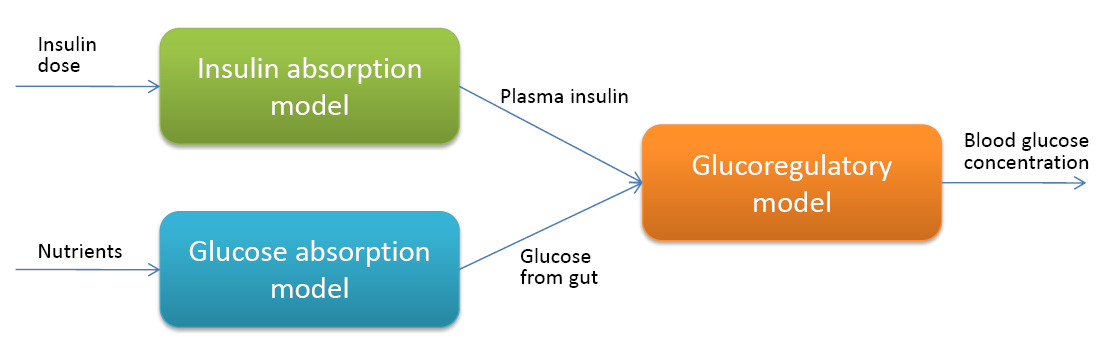
\epsfig{file=Figures/glucose_models.png, width=\textwidth}\caption{Glucose-insulin system and its sub-processes.}
\label{fig:glucosemodels}
\end{figure}

Subcutaneous insulin injection or pump delivery is the main control action to counteract disturbances like meal ingestion. Insulin pharmacokinetics has been studied for a long time, and the behavior of insulin analogues is well documented in literature. Complex glucose absorption models have been developed in the last years, but there still exist serious limitations to represent the physiological behavior of the digestive and intestinal absorption processes during a mixed meal mainly due to limitation of clinical data. The main difficulty in the characterization of the gastrointestinal model is that glucose absorption is only measurable with tracer methods \cite{basu2003use}, but few studies have been done in this area so far. The only experiments done in this area were not performed using real mixed meals, but instead the patients ate marked jelly with eggs and bacon. The influence of the nutritional composition is very relevant in the final model output, and it has not been taken in consideration so far.

Most commonly used models for the above mentioned systems will be introduced in the next sections, and later a critical review of the usefulness of these models will be performed in order to narrow down the scope of the research, not to forget that the last objective of this thesis is the identification of postprandial models for control.

\section{Insulin absorption models}
\label{sec:InsulinPharmacokineticsModels}

Modeling of subcutaneous (s.c.) insulin diffusion and absorption dates back to the 80's. Kobayashi \textit{et al.} published in 1983 a model based on a one-compartmental delay differential equation for U40 Actrapid insulin \cite{kobayashi1983pharmacokinetics} on type 1 and type 2 diabetic patients. Models proposed in literature have been increasing in complexity since then, like the two-compartmental model proposed by Kraegen \textit{et al.} in 1984 \cite{kraegen1984insulin}, or the model considering two different insulin pathways proposed by Puckett \textit{et al.} \cite{puckett1995model} in 1995. Increasing in complexity, Mosekilde \textit{et al.} proposed a model based on partial differential equations describing insulin dissociation, protein binding, diffusion and absorption \cite{Mosekilde1989modeling}. Later, Trajanoski \textit{et al.} simplified that model, and Tar\'in \textit{et al.} extended it's use to new insulin formulations, specifically to the insulin analog glargine \cite{tarin2005comprehensive}.

Works focused on the development of the artificial pancreas have studied in more detail the fast-acting insulin (e.g. lispro) used in insulin pumps. Wilinska \textit{et al.} from the University of Cambridge compared eleven different models for insulin lispro kinetics on data from seven patients with type 1 diabetes \cite{wilinska2005insulin}, concluding that the best performance was achieved by a model which considered two insulin absorption channels, a slow and a fast one. The group of Cambridge is one of the lead research teams for the artificial pancreas development, and they published a diabetic patient simulator in 2010 for \emph{in silico} testing of controllers \cite{simuladorhovorka}. However, a simplified version of the insulin absorption model was included, comprising a two-compartment single-path absorption structure, probably due to identifiability problems. The group of the University of Virginia and the University of Padova also published a simulator (henceforth UVA simulator) in 2007 \cite{magni2007model} with a very similar two compartment model. The models proposed by these two groups will now be displayed in more detail due to its widespread use.

\subsection{UVA model}
\label{sec:UVAins}

The model proposed by Dalla Man \textit{et al.} in 2007 \cite{man2007meal} has two compartments for the interstitial space and considers the elimination of insulin to happen entirely after the absorption to the plasma compartment. There are two variants of the model, depending on the complexity considered for the model of insulin distribution. The first and simpler model is the one shown in Figure \ref{fig:cobellisc1}. In this model, absorption takes place from both stages of the subcutaneous route.

\begin{figure}[hbtp]
\centering
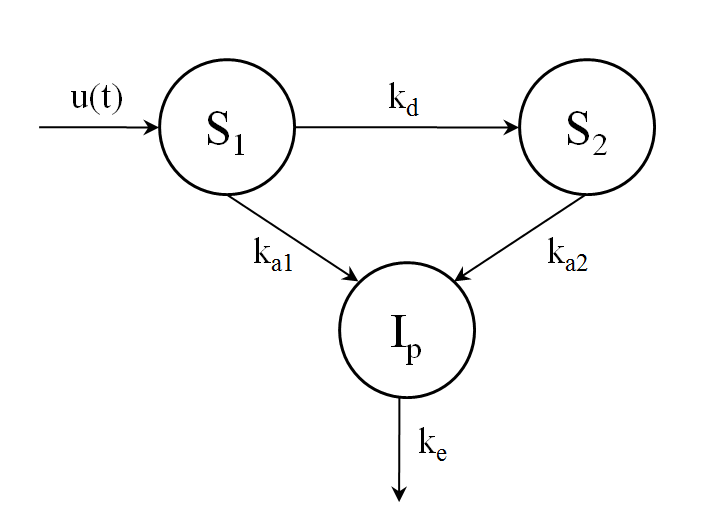
\epsfig{file=Figures/Cobelli1.png, width=0.6\textwidth}\caption{UVA model with one compartment for the insulin in plasma. Adapted from \cite{man2007meal}.}
\label{fig:cobellisc1}
\end{figure}

The equations related to the model are:
\begin{align}
	\dot{S}_{1}(t) &= -(k_{a1}+k_{d})S_{1}(t)+u(t) \label{eq:cobellisc1}\\
	\dot{S}_{2}(t) &= k_{d}S_{1}(t)-k_{a2}S_{2}(t) \label{eq:cobellisc2}\\
	\dot{I}_{p}(t) &= k_{a1}S_{1}(t)+k_{a2}S_{2}(t)-k_{e}I_{p}(t) \label{eq:cobellisc3}
\end{align}

where $S_{1}(t)$ and $S_{2}(t)$ are two compartments for the subcutaneous insulin absorption, $k_{a1}$, $k_{a2}$ and $k_{d}$ are the flux rates between compartments and plasma insulin ${I}_{p}(t)$, and $k_{e}$ is the insulin elimination rate. The insulin input is represented by the variable $u(t)$. Usually the subcutaneous part is used with a more complex insulin distribution and elimination model, also proposed by the Virginia and Padova group. The new model is displayed in Figure \ref{fig:cobellisc2}. In this case, elimination of insulin takes places both by degradation in the plasma compartment and in the liver. The influence of the liver is displayed by a new compartment.

\begin{figure}[hbtp]
\centering
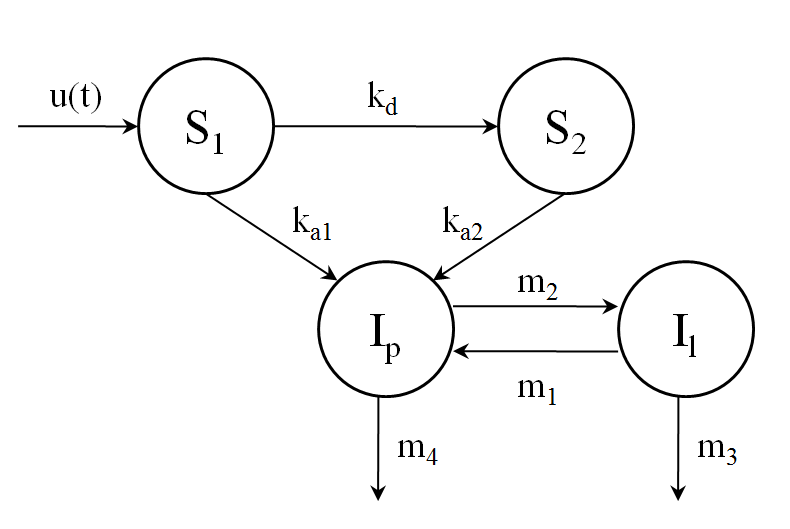
\epsfig{file=Figures/Cobelli2.png, width=0.6\textwidth}\caption{UVA model considering insulin in the liver and in plasma. Adapted from \cite{man2007meal}.}
\label{fig:cobellisc2}
\end{figure}

The corresponding system of equations related is very similar, but substituting equation \eqref{eq:cobellisc3}  with the following two differential equations:
\begin{align}
	\dot{I}_{l}(t) &= -(m_{1}+m_{3})I_{l}(t)+m_{2}I_{p}(t) \label{eq:cobellisc4}\\
	\dot{I}_{p}(t) &= -(m_{2}+m_{4})I_{p}(t)+m_{1}I_{l}(t)+ k_{a1}S_{1}(t)+k_{a2}S_{2}(t) \label{eq:cobellisc5}
\end{align}

where the plasma insulin elimination is replaced with a set of flux parameters ($m_1$, $m_2$, $m_3$ and $m_4$) and two dynamic states ($I_p$ and $I_l$) that represent insulin in plasma and the liver. Published values for T1DM patients were made available in 2008 in the international patent for the UVA simulator \cite{UVAsimpatente}. Public available values \cite{man2007meal} for healthy and T2DM patients for the distribution and elimination part of the model are shown in Table \ref{tab:cobelli_insulin}. Parameter $m_{3}$ does not appear in the table because it only is constant for T1DM patients while for the literature cases it presents dynamic behavior depending on the endogenous insulin secretion. Nevertheless, this model is implemented in the University of Virginia Simulator \cite{kovatchev2009biosimulation}, and nominal parameters for healthy and diabetic patients are used in glucose profiles simulated with it.

\begin{table}[hbtp]
	\centering
		\begin{tabular}{|c c c c|}
		\hline 
		Parameter &	Healthy value & T2DM value & Units \\
		\hline
		$m_{1}$ & $0.19$ & $0.379$ & min$^{-1}$ \\
		$m_{2}$ & $0.484$ & $0.673$ & min$^{-1}$ \\
		$m_{4}$ & $0.194$ & $0.269$ & min$^{-1}$ \\
		\hline		
		\end{tabular}
	\caption{Published values of the UVA s.c. insulin model.}
	\label{tab:cobelli_insulin}
\end{table}

\subsection{Cambridge model}
\label{sec:WillinskaEtAl}

In 2005 Willinska compared eleven subcutaneous models of increasing complexity \cite{wilinska2005insulin}. Those models where evaluated for bolus-basal treatments and continuous infusion with insulin pumps with insulin \textit{lispro}, a human insulin analog. The structure of the model with a better fit to experimental data is shown in Figure \ref{fig:willinska}.

\begin{figure}[hbtp]
\centering
\epsfig{file=Figures/Willinska.png, width=0.8\textwidth}\caption{Cambridge's model compartmental structure.Adapted from \cite{wilinska2005insulin}.}
\label{fig:willinska}
\end{figure}

The equations of the model are:
\begin{align}
	\dot{Q}_{1a}(t) &= ku(t)-k_{a1}Q_{1a}(t)-LD_{a}(t) \label{eq:Willinska1}\\
	\dot{Q}_{1b}(t) &= (1-k)u(t)-k_{a2}Q_{1b}(t)-LD_{b}(t) \label{eq:Willinska2}\\
	\dot{Q}_{2}(t) &= k_{a1}Q_{1a}(t)-k_{a1}Q_{2}(t)\label{eq:Willinska3}\\
	\dot{Q}_{3}(t) &= k_{a1}Q_{2}(t)+k_{a2}Q_{1b}(t)-k_{e}Q_{3}(t)\label{eq:Willinska4}\\
	I(t) &= \frac{Q_{3}(t)}{V_i\cdot BW} \label{eq:Willinska5}\\
	LD_{a}(t) &= \frac{V_{MAX,LD}Q_{1a}(t)}{k_{M,LD}+Q_{1a}(t)}\label{eq:Willinska6}\\
	LD_{b}(t) &= \frac{V_{MAX,LD}Q_{1b}(t)}{k_{M,LD}+Q_{1b}(t)}\label{eq:Willinska7}
\end{align}

The most significant characteristic of this model is the existence of two channels of insulin, one of slow absorption and a fast absorption insulin channel, both with degradation of insulin ruled by a Michaelis-Menten kinetic equation. ${Q}_{1a}(t)$ and ${Q}_{1b}(t)$ are the states related to slow insulin distribution in the subcutaneous tissue, ${Q}_{2}(t)$ is the state related to the fast distribution channel, and ${Q}_{3}(t)$ is directly related to the plasma insulin. $LD_{a}(t)$ and $LD_{ab}(t)$ describe insulin degradation with the constant parameters $V_{MAX,LD}$ and $k_{M,LD}$, $V_i$ is the insulin distribution volume, $BW$ is the patient's body weight and finally $k_{a1}$, $k_{a2}$ and $k_{e}$ are the constant fluxes and elimination rates between insulin compartments. The insulin concentration is directly calculated from the fourth compartment. Published parameters of the model are shown in Table \ref{tab:Willinska}.

\begin{table}[hbtp]
	\centering
		\begin{tabular}{|c c c|}
		\hline 
		Parameter &	Published value & Units \\
		\hline
		$k_{a1}$ & $1.12\cdot 10^{-2}$ & min$^{-1}$ \\
		$k_{a2}$ & $2.1\cdot 10^{-2}$ & min$^{-1}$ \\
		$k_{e}$ & $1.89\cdot 10^{-2}$ & min$^{-1}$ \\
		$k$ & $0.67$ & - \\
		$V_i$ & $56.45\cdot 10^{-2}$ & L kg$^{-1}$ \\
		$V_{MAX,LD}$ & $1.93$ & mU min$^{-1}$ \\
		$k_{M,LD}$ & $62.6$ & mU \\
		\hline		
		\end{tabular}
	\caption{Nominal values of the parameters in Willinska's model.}
	\label{tab:Willinska}
\end{table}

In the simulator published in 2010 \cite{simuladorhovorka} the Cambridge group implemented a much simpler linear compartmental model. The model structure is shown in Figure \ref{fig:willinska_simulator}.

\begin{figure}[hbtp]
\centering
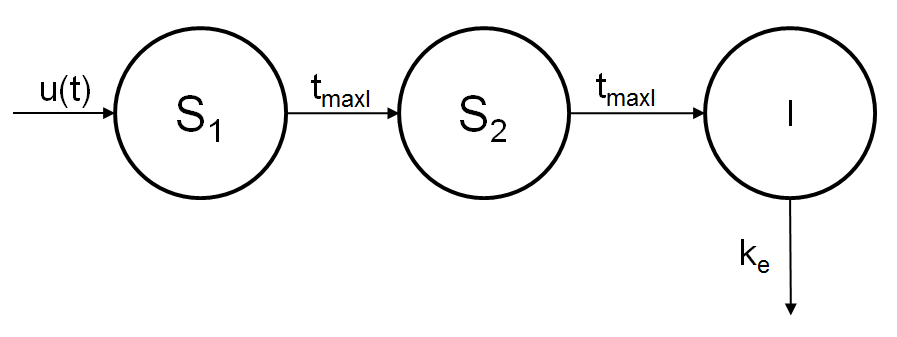
\epsfig{file=Figures/willinska_simulador.png, width=0.6\textwidth}\caption{Cambridge simulator insulin absorption model structure. Adapted from \cite{simuladorhovorka}.}
\label{fig:willinska_simulator}
\end{figure}

This model displays a simple flow of insulin through two compartments into the bloodstream, and it only considers elimination of insulin from blood. The flow constants between compartments is the same. The equations of this model are shown next:
\begin{align}
	\dot{S}_{1}(t) &= u(t)-t_{maxI}S_{1}(t) \label{eq:Willinska_simulator1}\\
	\dot{S}_{2}(t) &= t_{maxI}S_{1}(t)-t_{maxI}S_{2}(t) \label{eq:Willinska_simulator2}\\
	\dot{I}(t) &= \frac{t_{maxI}S_{2}(t)}{V_{i}}-k_{e}I(t)\label{eq:Willinska_simulator3}
\end{align}

The insulin compartment $I(t)$ is directly the insulin concentration. There are three parameters in this model: $t_{maxI}$ is the insulin absorption rate, $k_{e}$ is the elimination rate from the blood compartment, and $V_{i}$ is the insulin distribution. Willinska \textit{et al.} presented probability distributions of these parameters calculated from a population of 18 type 1 diabetic patients. For sake of simplicity and uniformity only mean values will be shown in this manuscript in Table \ref{tab:Willinska_simulador}, but the complete distributions can be found in \cite{simuladorhovorka}.

\begin{table}[hbtp]
	\centering
		\begin{tabular}{|c c c|}
		\hline 
		Parameter &	Published value & Units \\
		\hline
		$t_{maxI}$ & $0.018$ & min$^{-1}$ \\
		$k_{e}$ & $0.14$ & min$^{-1}$ \\
		$V_{i}$ & $0.12$ & L kg$^{-1}$ \\
		\hline		
		\end{tabular}
	\caption{Mean values of the parameters in the Cambridge simulator model.}
	\label{tab:Willinska_simulador}
\end{table}

\section{Glucose absorption models}	
\label{sec:GlucoseAbsorptionModels}

Glucose absorption models aim at characterizing the flux of exogenous glucose absorbed from the intestine under different circumstances taking under consideration the information on the meal intake. Modeling meal absorption has been proven difficult due to complex physiology of gastric emptying and intestinal absorption. The nature of the meal, its size and composition, as well as the speed of ingestion, and patient conditions, have influence on the rate of stomach emptying \cite{mitchell1989gastric} and the final absorption rate of glucose. Large variability was reported by Klingensmith \textit{et al.} \cite{klingensmith2010gastric} even within the same patient and meal. Furthermore, the rate of appearance of glucose in the bloodstream is not directly measurable (unlike blood insulin concentration in the insulin absorption models) which hardens the modeling endeavor.

One of the first models proposed in literature was an exponential model for gastric emptying presented in \cite{hunt1975volume}, where the emptying rate is dependent on the meal's volume and calorie density. After the contribution by Hunt \textit{et al.} most of the published models express the dynamics of glucose appearance as a function of the carbohydrate content of the meal. In 1992 Lehman and Deutch \cite{lehmann1992physiological} proposed a trapezoidal emptying of the stomach based on the carbohydrates ingested neglecting the influence of other nutrients. In 2006 Fabietti \textit{et al.} \cite{fabietti2006control} proposed an input-output model based on the different absorption rates of mono- and polysaccharides. A model independent approach was proposed by Herrero \textit{et al.} in \cite{bibliotecapau}, where the glucose absorption profile was extracted from a library comprehending several mixed meals and different patients. Also, deconvolution methods have been applied in order to infer the glucose absorption profile as proposed in \cite{herrero2012simple}.

In the simulators published up to date, physiological compartmental models are usually implemented. In the following lines we will describe in detail glucose absorption models from the UVA and Cambridge groups.

\subsection{UVA model}
\label{sec:ModelBasedOnDallaManEtAl}

Chiara Dalla Man \textit{et al.} published in 2006 a complete gastrointestinal model along with a critical review of the existing models in literature \cite{man2006system}. This model considers a two-compartment model for digestion and a simple single-compartmental model for the absorption in the gut. To overcome the issue of the measurability of glucose rate of appearance from the gut the UVA group used data from a triple tracer study, allowing for the estimation of glucose absorption, although in healthy subjects. The model follows the structure shown in Figure \ref{fig:dallaman}.

\begin{figure}[hbtp]
\centering
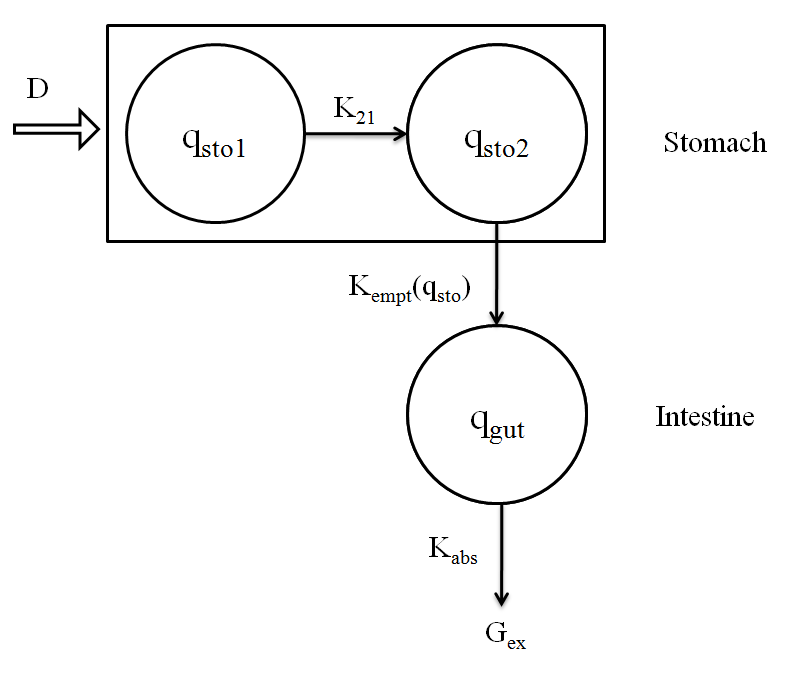
\epsfig{file=Figures/dallaman.png, width=0.6\textwidth}\caption{A two compartment model represents the stomach and a single compartment the intestine. Adapted from \cite{man2006system}.}
\label{fig:dallaman}
\end{figure}

The two compartments in the stomach part ($q_{sto1}$ and $q_{sto2}$) represent the solid and liquid phase of carbohydrate digestion before the gastric emptying. The emptying of the stomach is a non-linear function of the total amount of glucose in the stomach, as will be shown in the model equations later. The compartmental model equations are:
\begin{align}
  \dot{q}_{sto1}(t) &=-K_{21}q_{sto1}(t)+D\delta (t)\label{eq:dallaman1}\\
  \dot{q}_{sto2}(t) &=-K_{empt}(q_{sto})q_{sto2}(t)+K_{21}q_{sto1}(t)\label{eq:dallaman2}\\
  \dot{q}_{gut}(t) &=-K_{abs}q_{gut}(t)+K_{empt}(q_{sto})q_{sto2}(t)\label{eq:dallaman3}\\
  G_{ex}(t) &=fK_{abs}q_{gut}(t)\label{eq:dallaman4}
\end{align}
where $\delta (t)$ is the Dirac delta and $D$ is the meal size, simulating an impulse input to the model. $f$ stands for the bio-availability of the meal. The rest of parameters added ($K_{21}$ and $K_{abs}$) are flux constants between compartments, for characterization of the transfer of glucose through the system, except for the $K_{empt}$ parameter, which is time-varying and defines the form of the gastric emptying. The equations describing the transfer rate describing the flow of glucose from the stomach to the intestine are:
\begin{equation} \label{eq:dallaman5}
\begin{array}{ll}
  K_{empt}(q_{sto}) &= K_{min}+\frac{K_{max}-K_{min}}{2}\cdot\\
  & \hskip -1.5cm \cdot \{ tanh[\alpha (q_{sto}(t)-b\cdot D)]-tanh[\beta (q_{sto}(t)-c\cdot D)]+2\}\\
\end{array}
\end{equation}
\begin{equation} \label{eq:dallaman6}
  q_{sto}(t) =q_{sto1}(t)+q_{sto2}(t)\\
\end{equation}
\begin{equation} \label{eq:dallaman7}
  \alpha = \frac{5}{2D(1-b)}; \qquad   \beta = \frac{5}{2Dc} \\
\end{equation}
These equations give the gastric emptying a very characteristic shape. In Figure \ref{fig:dallaman2} the $K_{empt}$ is plotted against the amount of glucose remaining in the stomach $q_{sto}$.

\begin{figure}[hbtp]
\centering
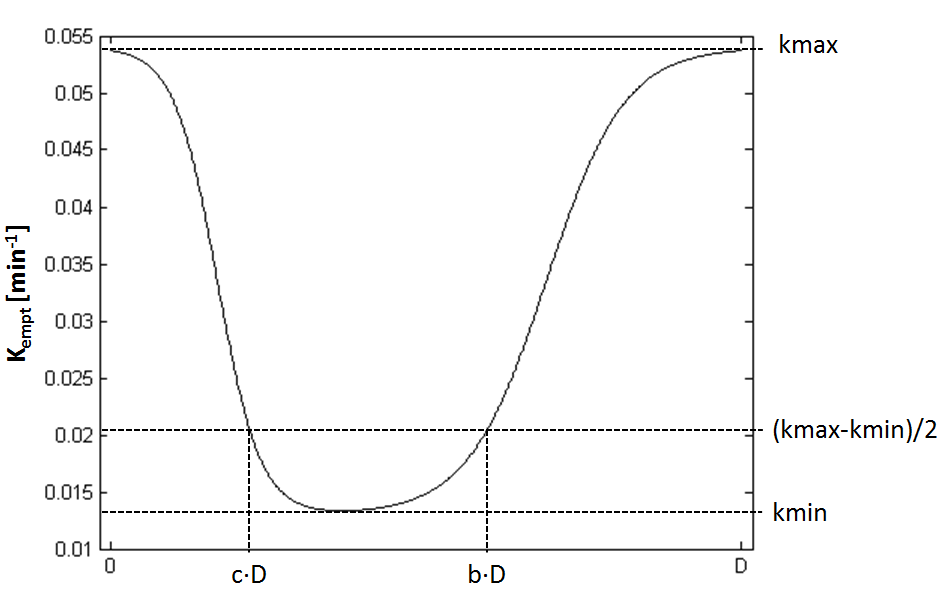
\epsfig{file=Figures/dallaman2.png, width=0.8\textwidth}\caption{Gastric emptying rate versus glucose remaining in the stomach. Adapted from \cite{man2006system}.}
\label{fig:dallaman2}
\end{figure}

$K_{max}$ and $K_{min}$ are the maximum and minimum emptying rates through the digestion process, while $b$ and $c$ are geometric parameters describing the shape of the gastric emptying. The parameters shown next have been identified both for an Oral Glucose Tolerance Test (OGTT, consisting in 75g of oral glucose ingestion according to the World Health Organization recommendation) and a mixed meal, although the mixed meal consisted only of traced jelly with eggs and bacon. Parameter $K_{21}$ is forced to be equal to $K_{max}$ for identifiability issues. The published values are shown in Table \ref{tab:dallaman}.

\begin{table}[hbtp]
	\centering
		\begin{tabular}{|c c c c|}
		\hline 
		Parameter & Published value (OGTT) & Published value (meal) & Units \\
		\hline 
		$K_{abs}$ & $0.205$ & $0.071$ & min$^{-1}$ \\
		$K_{21}$ & $0.045$ & $0.054$ & min$^{-1}$ \\
		$K_{max}$ & $0.045$ & $0.054$ & min$^{-1}$ \\
		$K_{min}$ & $0.013$ & $0.006$ & min$^{-1}$ \\
		$b$ & $0.85$ & $0.69$ & - \\
		$c$ & $0.25$ & $0.17$ & - \\
		\hline
		\end{tabular}
	\caption{Nominal values of the parameters in the UVA model.}
	\label{tab:dallaman}
\end{table}

%Some work has been done within this research group on identifiability of mixed meals with the Dalla Man model \cite{tesinacrisos}, showing a dependence of the identification results on the size of the meal considered.

\subsection{Cambridge model}
\label{sec:ModelBasedOnHovorkaEtAl}

Hovorka \textit{et al.} proposed a simple model for glucose absorption in 2004 \cite{hovorka2004nonlinear}, where the gastrointestinal system is modeled by two identical compartments with the same transfer rate. Later, the model was refined \cite{simuladorhovorka} considering the transfer rate $t_{max}$ as a time-varying parameter. The equations of the model are:
\begin{align}
	\dot{G}_{1}(t) &=-\frac{G_{1}(t)}{t_{max}}+Bio\cdot D(t) \label{eq:hovorkagut1}\\
	\dot{G}_{2}(t) &=\frac{G_{1}(t)}{t_{max}}-\frac{G_{2}(t)}{t_{max}} \label{eq:hovorkagut2}\\
	G_{ex}(t) &=\frac{G_{2}(t)}{t_{max}} \label{eq:hovorkagut3}
\end{align}
where:
\begin{itemize}
	\item \textbf{$D(t)$} is the amount of carbohydrates ingested in grams. The meal intake in this model is considered as a pulse input.
	\item \textbf{$Bio$} is the effectiveness of the absorption of the carbohydrates ingested, i.e. the portion of the carbohydrates that have been eaten that will go into the circulatory system (Bioavailability).
	\item \textbf{$t_{max}$} is the maximum absorption time of the carbohydrates. This parameter regulates the transfer speed between the compartments. It is a bounded parameter following:
	\begin{equation} 
	  t_{max}=\left\{ \begin{array}{cc} 
	  t_{max\ ceil} & \mbox{ if } G_{ex} > G_{ex\ ceil} \\ 
	  t_{max} & \mbox{ otherwise } \\	
	  \end{array} \right.
	\label{eq:hovorkagut4}
	\end{equation}
	where $t_{max\ ceil}=\frac{G_{2}}{G_{ex\ ceil}}$ and $G_{ex\ ceil}$ is the maximum glucose flux from the gut.
	\item \textbf{$G_{ex}(t)$} is the output of the model, as a flux of glucose from the gut. $G_{1}(t)$ and $G_{2}(t)$ are the transition compartments for glucose in the disgestion process.
\end{itemize}
The nominal values of the parameters are shown in Table \ref{tab:hovorkagut}.

\begin{table}[hbtp]
	\centering
		\begin{tabular}{|c c c|}
		\hline 
		Parameter & Published value & Units \\
		\hline 
		$t_{max}$ & $40$ & min \\
		$Bio$ & $0.8$ & - \\
		$G_{ex\ ceil}$ & $[0.02, 0.035]$ & mmol kg$^{-1}$ min$^{-1}$ \\
		\hline
		\end{tabular}
	\caption{Nominal values of the parameters in Hovorka model.}
	\label{tab:hovorkagut}
\end{table}

This model has the weakness of not considering the different compositions of mixed meals, as other models do, but it computes a very simple input for the glucoregulatory system in the simulation environment.

\section{Endogenous models}
\label{sec:EndogenousModels}

The endogenous model is the part of the glucose-insulin model that describes the different regulatory metabolic pathways of blood glucose concentration. Given that this thesis is focusing in the identification of glucose metabolism for T1DM subjects, the author decided that the dynamics and equations describing the secretion of insulin were no relevant to be shown for those models that describe it, since it does not exist in type 1 diabetes.

Usually the endogenous model comprises two sub-models: (1) insulin pharmacodynamics and (2) glucose metabolism and distribution. This second sub-model has to consider the influence of the liver and the kidneys on the blood glucose production and elimination, as well as the peripheral intake by muscles and adipose tissue, and any other influences that may affect glucose concentration. 

Two different groups of models will be described next. The first two models (Bergman and Panunzi) are considered as \textit{minimal} models, and are very simple models that do not attempt at simulating the whole metabolic system of glucose regulation but to capture the main dynamics in specific assays like the Intra Venous Glucose Tolerance Test (IVGTT) for insulin sensitivity estimation. Minimal models are widely used for research either in simulation studies or for control, but lack the accuracy of more complex models. The other two models reviewed next are physiology-based models developed by the UVA group and the Cambridge group, and are much more complex than the previous ones, aiming at population studies for controllers validation.

\subsection{Bergman model}
\label{sec:BergmanEtAl}

The first model to be reviewed is the (probably) most used and best known among all the endogenous models used in diabetes. It was proposed by Bergman \textit{et al.} in 1981 \cite{bergman1981physiologic}. It is considered a minimal model because it only describes the influence of insulin on blood glucose concentration, and it does not consider many other phenomena, or it considers them in a very simplified way, leading to a low order model. The justification for this simplicity is that the objective of this model was, initially, to simulate the response of the IVGTT, which has a very simple behavior.

Bergman minimal model considers that insulin actions on glucose are delayed, and that delay is represented by a new compartment of \textit{remote} insulin. The scheme of the model is shown in Figure \ref{fig:bergman1}.

\begin{figure}[hbtp]
\centering
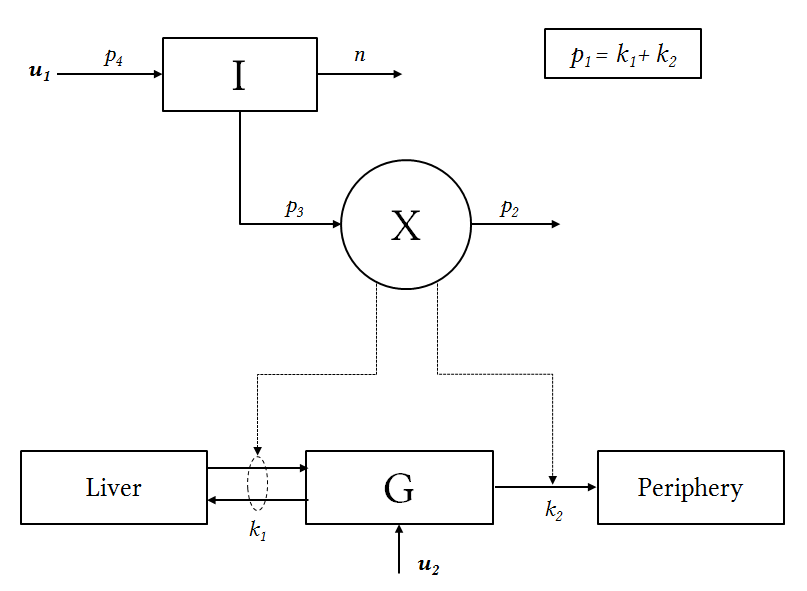
\epsfig{file=Figures/bergman.png, width=0.8\textwidth}\caption{Bergman minimal model of insulin and glucose dynamics. Adapted from Bergman and colleagues \cite{bergman1981physiologic}.}
\label{fig:bergman1}
\end{figure}

The equations that describe the model are:
\begin{align}
  \dot{I}(t) &= -nI(t)+p_{4}u_{1}(t) & I(0)=I_{b}=\frac{p_{4}}{n}u_{1b} \label{eq:Bergman1}\\
  \dot{X}(t) &= -p_{2}X(t)+p_{3}[I(t)-I_{b}] & X(0)=0 \label{eq:Bergman2}\\
  \dot{G}(t) &= -p_{1}G(t)-X(t)G(t)+p_{1}G_{b} + \frac{u_{2}(t)}{V_{G}} & G(0)=G_{b} \label{eq:Bergman3}
\end{align}

where the insulin compartment is described by the state $I(t)$, with parameters $p_4$ and $n$ involved in the insulin input and elimination respectively. Parameters $p_3$ and $p_2$ describe the input and output fluxes for the remote insulin compartment $X(t)$, and finally glucose difusion and transportation is gobernated by parameter $p_1$, which is a compound parameter involving both liver interaction ($k_1$) and usage by periphery ($k_2$). For subcutaneous insulin absorption, equation \eqref{eq:Bergman1} would be substituted by the corresponding model in Section \ref{sec:InsulinPharmacokineticsModels}. $G(t)$ is the blood glucose concentration, $u_{1}(t)$ is the exogenous insulin flow entering circulation, $u_{2}(t)$ is the exogenous flow of glucose coming either intravenously or from the gastrointestinal system. Published values for the model parameters are shown in Table \ref{tab:Bergman}.

\begin{table}[hbtp]
	\centering
	\begin{tabular}{|c c c|}
	\hline 
	Parameter & Published value & Units \\
	\hline 
	$p_{1}$ & $0.035$ & min$^{-1}$ \\
	$p_{2}$ & $0.05$ & min$^{-1}$ \\
	$p_{3}$ & $0.000028$ & ml$/\mu U\cdot$ min$^{2}$ \\
	$p_{4}$ & $0.098$ & ml$^{-1}$ \\
	$n$ & $0.142$ & min$^{-1}$ \\
	$V_{G}$ & $117$ & dl\\
	\hline
	\end{tabular}
\caption{Nominal values of the parameters in Bergman model \cite{roy2007dynamic}.}
\label{tab:Bergman}
\end{table}

Bergman model has been used for more than 20 years in diabetes research due to its identifiability and controllability properties, despite its simplicity. Nevertheless, Bergman model will be analyzed in detail in Section \ref{sec:BergmanEtAl}.

\subsection{Panunzi model}
\label{sec:PanunziEtAl}

Simona Panunzi \textit{et al.} published a study in 2007 comparing some of the characteristics of Bergman model and new features of a proposed model for the IVGTT scenario, with a delayed insulin secretion rate \cite{panunzi2007discrete}. The new model proposed surpassed the rest in simulated experiments and in identifiability properties, but it was only tested in healthy patients. The equations of the model are:
\begin{align}
  \dot{G}(t) &= -K_{xgl}I(t)G(t) +\frac{T_{gh}}{V_{g}} \label{eq:Panunzi1} \\
  \dot{I}(t) &= -K_{xi}I(t)+\frac{T_{ig\ max}}{V_{i}}\frac{\left(\frac{G(t-\tau_{g})}{G^{*}}\right)^{\gamma}}{1+\left(\frac{G(t-\tau_{g})}{G^{*}}\right)^{\gamma}} \label{eq:Panunzi2}
\end{align}
This model includes delayed differential equations for the insulin production sub-model, but when simulating type 1 diabetic patients, whom do not have endogenous insulin secretion, the model becomes much more simple. The parameters involved in the previous model are:
\begin{itemize}
	\item \textbf{$G_{b}$} is the basal glucose concentration.
	\item \textbf{$I_{b}$} is the basal plasma insulin.
	\item \textbf{$K_{xgl}$} is the insulin sensitivity. It represents the insulin-dependent glucose uptake by tissues per unit of insulin concentration.
	\item \textbf{$T_{gh}$} represents the balance between the hepatic glucose production of glucose and the insulin-independent glucose intake, including the one of the liver.
	\item \textbf{$V_{g}$} is the apparent glucose distribution volume.
	\item \textbf{$K_{xi}$} is the disappearance rate of insulin.
	\item \textbf{$G^{*}$} is the glycemia at which the insulin secretion rate is half of its maximum.
	\item \textbf{$T_{ig\ max}$} is the maximum rate of insulin release.
	\item \textbf{$V_{i}$} is the apparent insulin distribution volume.
	\item \textbf{$\tau_{g}$} represents the apparent delay with which the pancreas changes insulin release in response to a variation in blood glucose.
	\item \textbf{$\gamma$} is the progressivity with which the pancreas reacts to circulating glucose concentrations.
\end{itemize}
The values published for these parameters, only for healthy patients, are shown in Table \ref{tab:panunzi}.

\begin{table}[hbtp]
	\centering
		\begin{tabular}{|c c c|}
		\hline 
		Parameter & Published value & Units \\
		\hline 
		$V_{g}$ & $0.152$ & L\ kg$^{-1}$ \\
		$\tau_{g}$ & $19.271$ & min \\
		$K_{xgl}$ & $1.43\times 10^{-4}$ & min$^{-1}$ \ pM$^{-1}$ \\
		$K_{xi}$ & $0.101$ & min$^{-1}$ \\
		$\gamma$ & $2.464$ & - \\
		\hline
		\end{tabular}
	\caption{Nominal values of the parameters in Panunzi model.}
	\label{tab:panunzi}
\end{table}

Panunzi model is also used later in this thesis because of its simplicity, but some variations were made in Chapter \ref{sec:CriticalSelectionOfModels} due to the focus of this model on healthy patients and the IVGTT scenario, and in order to extend its use to diabetic patients.

\subsection{UVA model}
\label{sec:CobelliEtAl}

The core of the UVA model was presented in \cite{man2007meal}, and it is one of the most important models in diabetes research. It is a very complex model almost exclusively based on physiological knowledge of the glucose metabolism. It is usually combined with the UVA gastrointestinal model and the insulin pharmacokinetics model of the same group (in fact all the models were developed together) in a large mathematical model of the glucose metabolism. Magni \textit{et al.} \cite{magni2007model} used a linearization of the UVA model to control an \textit{in silico} diabetic patient. It is also the model implemented in the UVA simulator \cite{kovatchev2009biosimulation} which was accepted by the FDA (Food \& Drug Administration) as substitute of animal trials in the context of a controller validation trial by University of Virginia and Padova. The core structure is pretty simple, as shown in Figure \ref{fig:cobelliendo}:

\begin{figure}[hbtp]
\centering
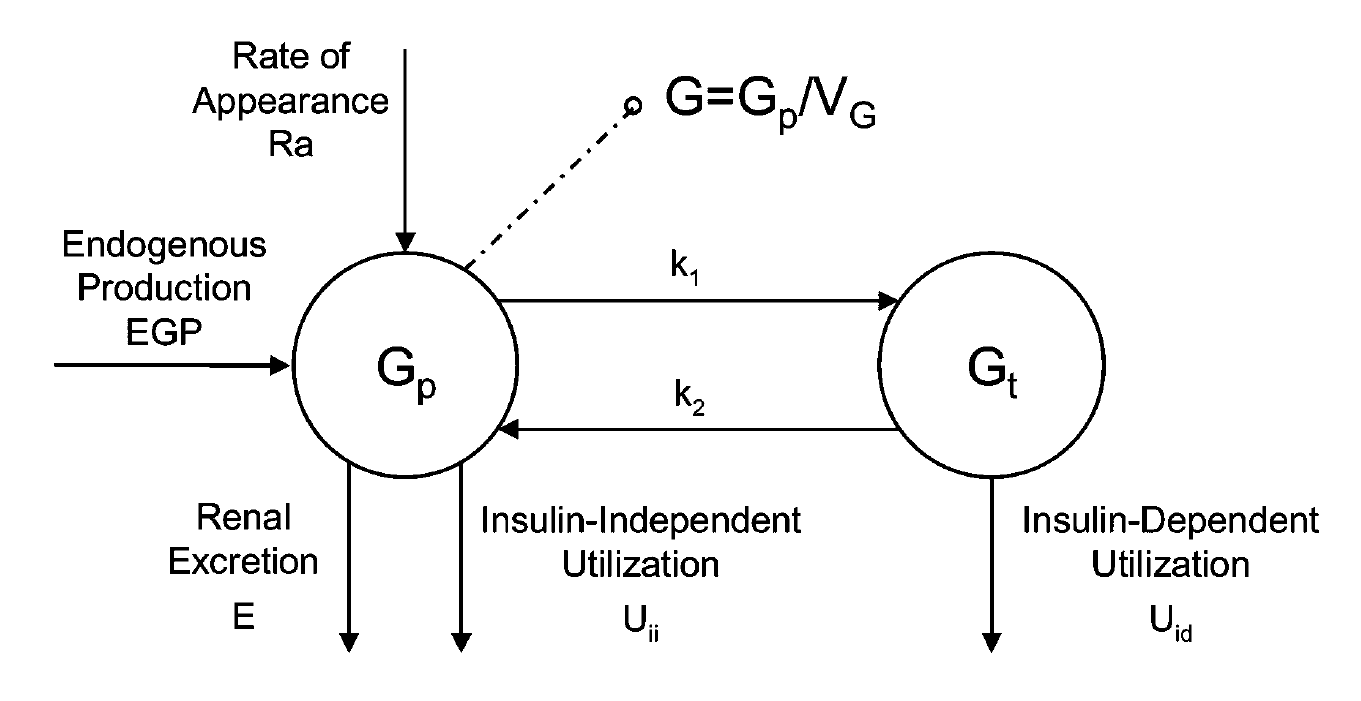
\epsfig{file=Figures/cobelliendo.png, width=0.8\textwidth}\caption{UVA's model core is composed of two compartments of glucose, one for blood and one for the tissues interstitial fluid. Schematics adapted from \cite{man2007meal}}
\label{fig:cobelliendo}
\end{figure}

The model equations are:
\begin{align}
  \dot{G}_{p}(t) &= EGP(t) + Ra(t) - U_{ii}(t) - E(t) - k_{1}G_{p}(t) + k_{2}G_{t}(t) \label{eq:cobelli1} \\
  \dot{G}_{t}(t) &= -U_{id}(t) + k_{1}G_{p}(t) - k_{2}G_{t}(t) \label{eq:cobelli2} \\
  G(t) &=G_{p}(t)/V_{G} \label{eq:cobelli3}
\end{align}
In the previous equations there are many inputs and outputs to the glucose compartments that need description. It must be noted that so far there are no insulin related equations; insulin influences the flow of glucose coming in or out of the different compartments. The meaning of these variables is explained next:
\begin{itemize}
	\item $Ra$ is the exogenous flux of glucose coming from the gut.
	\item $U_{ii}$ is the utilization of glucose that is non dependent on insulin. It is usually considered constant and equal to $F_{cns}$. 
	\item $U_{id}$ is the utilization that depends on the insulin concentration, and it follows the following set of equations:
  \begin{align}
  	\dot{X}(t) &= -p_{2U}X(t)+p_{2U}[I(t)-I_{b}]\label{eq:cobelli4} \\
  	V_{m}(X(t)) &= V_{m0}+V_{mx}X(t) \label{eq:cobelli5} \\
		U_{id}(t) &= \frac{V_{m}(X(t))G_{t}(t)}{K_{m}+G_{t}(t)} \label{eq:cobelli6}
	\end{align}	
	where $X(t)$ is the remote insulin, $I(t)$ is the plasma insulin, $I_{b}$ is the basal insulin and $V_{m}(t)$ is the transfer rate for the Michaelis-Menten equation shown in equation \eqref{eq:cobelli6}.
  \item $E(t)$ represents the renal excretion, which occurs if plasma glucose exceeds a certain threshold. It is modeled as follows:
  \begin{equation}
	E(t) = \left\{
		\begin{array}{cc} k_{e1}[G_{p}(t)-k_{e2}] & \mbox{ if } G_{p}(t)>k_{e2} \\
		0 &\mbox{ otherwise } 
		\end{array} \right.
  \label{eq:cobelli7}
  \end{equation}
  where $k_{e1}$ is the glomerular filtration rate and $k_{e2}$ is the renal threshold of glucose.
  \item $EGP(t)$ is the Endogenous Glucose Production, and it depends on a delayed insulin signal as follows:
  \begin{align}
  	\dot{I}_{1}(t) &= -k_{i}[I_{1}(t)-I(t)] \label{eq:cobelli8} \\
  	\dot{I}_{d}(t) &= -k_{i}[I_{d}(t)-I_{1}(t)] \label{eq:cobelli9} \\
		EGP(t) &= max\{0,k_{p1}-k_{p2}G_{p}(t)-k_{p3}I_{d}(t)\} \label{eq:cobelli10}
	\end{align}
	where $I(t)$ is the insulin concentration in plasma, $I_d(t)$ is the delayed insulin action, $k_i$ is the insulin delay flux rate and $k_{p1}$, $k_{p2}$ and $k_{p3}$ are constant parameters that describe $EGP$.
\end{itemize}
The published parameters for healthy and type 2 diabetic patients are those in Table \ref{tab:cobelli}. %Even though the parameters shown are those of healthy and T2DM patients, no endogenous production of glucose has been described in here for this model, which is the case of a T1DM person. 
\begin{table}[hbtp]
	\centering
		\begin{tabular}{|c c c c|}
		\hline 
		Parameter & Healthy & Type 2 diabetes & Units \\
		\hline 
		$V_{G}$ & $1.88$ & $1.49$ & dL\ kg$^{-1}$ \\
		$k_{1}$ & $0.065$ & $0.042$ & min$^{-1}$ \\
		$k_{2}$ & $0.079$ & $0.071$ & min$^{-1}$ \\
		$k_{p1}$ & $2.70$ & $3.09$ & mg\ kg$^{-1}$\ min$^{-1}$ \\
		$k_{p2}$ & $0.0021$ & $0.0007$ & min$^{-1}$ \\
		$k_{p3}$ & $0.009$ & $0.005$ &  mg\ kg$^{-1}$\ min$^{-1}$ per pmol L$^{-1}$ \\
		%$k_{p4}$ & $0.0618$ & $0.0786$ & mg\ kg$^{-1}$\ min$^{-1}$ per pmol kg$^{-1}$ \\
		$k_{i}$ & $0.0079$ & $0.0066$ & min$^{-1}$ \\
		$F_{cns}$ & $1$ & $1$ &  mg\ kg$^{-1}$\ min$^{-1}$ \\
		$V_{m0}$ & $2.5$ & $4.65$ &  mg\ kg$^{-1}$\ min$^{-1}$ \\
		$V_{mx}$ & $0.047$ & $0.034$ &  mg\ kg$^{-1}$\ min$^{-1}$ per pmol L$^{-1}$ \\
		$K_{m0}$ & $225.59$ & $466.21$ & mg\ kg$^{-1}$ \\
		$p_{2U}$ & $0.0331$ & $0.0840$ & min$^{-1}$ \\
		$k_{e1}$ & $0.0005$ & $0.0007$ & min$^{-1}$ \\
		$k_{e2}$ & $339$ & $269$ & mg\ kg$^{-1}$ \\
		\hline
		\end{tabular}
	\caption{Nominal values of the parameters in Cobelli model.}
	\label{tab:cobelli}
\end{table}

This model has been used in several experimental settings for closed-loop controller testing. Kovatchev \textit{et al.} published a study on 20 T1DM patients using an MPC controller tuned with the UVA simulator \cite{kovatchev2010multinational} \cite{clarke2009closed}. Improvement was reported in hypoglycemic events occurrence and in the amount of time spent in euglycemic range. Currently, the UVA group is performing home control experiments using controllers designed with this model.

An update of the UVA model and its simulator was published in January 2014 \cite{dalla2014uva}. The model is still based on the previous equations, but glucagon kinetics are included using a single compartment model. In order to simulate different glucose utilization depending on the glycemic region, the updated model includes a new glucose utilization module that depends on the risk of hypoglycemia. These last updates were not subject to examination in this thesis.

\subsection{Cambridge model}
\label{sec:HovorkaEtAl}

The Cambridge group proposed an endogenous model with split focus on three insulin actions and its final effect on blood glucose \cite{hovorka2002partitioning}. The model considers the following insulin effects:
\begin{itemize}
  \item Insulin increases the flow of glucose from blood to the tissues.
  \item Insulin increases the glucose uptake by muscles and adipose tissue.
  \item Insulin inhibits production of glucose in the liver.
\end{itemize}
These three influences are reflected in the model as virtual compartments. The relation between actual insulin in plasma, every virtual compartment representing insulin actions and the two compartments for glucose is shown in Figure \ref{fig:hovorka}. $x_{1}$, $x_{2}$ and $x_{3}$ represent the insulin actions, $Q_{1}$ is the glucose mass in the accessible compartment, and $Q_{2}$ is the glucose present in the non-accessible compartment. 

\begin{figure}[hbtp]
\centering
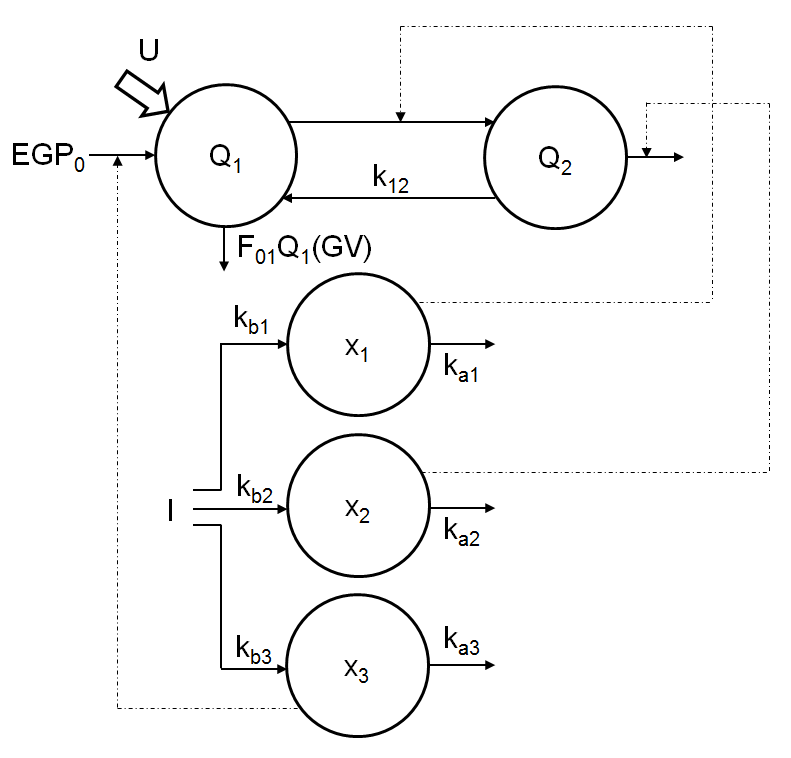
\epsfig{file=Figures/hovorka.png, width=0.8\textwidth}\caption{Hovorka endogenous model structure arranged in compartments. Adapted from \cite{hovorka2002partitioning}.}
\label{fig:hovorka}
\end{figure}

The equations that represent this model are:
\begin{align}
  \dot{x}_{1}(t) &= -k_{a1}x_{1}(t) + k_{b1}I(t) &  x_{1}(0)=0 \label{eq:hovorka1} \\
  \dot{x}_{2}(t) &= -k_{a2}x_{2}(t) + k_{b2}I(t) &  x_{2}(0)=0 \label{eq:hovorka2} \\
  \dot{x}_{3}(t) &= -k_{a3}x_{3}(t) + k_{b3}I(t) &  x_{3}(0)=0 \label{eq:hovorka3}
\end{align}

where $x_1(t)$, $x_2(t)$ and $x_3(t)$ are the three different insulin actions. These actions are used as inputs to the actual endogenous model.
%\begin{align}
%	\dot{Q}_{1}(t) &= -\left[\frac{F_{01}^{c}(t)}{V_{G}G(t)}+x_{1}(t)\right]Q_{1}(t)+k_{12}Q_{2}(t)-&F_{R}(t)+EGP(t)+&G_{ex}(t) \nonumber \\ 
%	& & Q_{1}(0)=Q_{1,0}& \label{eq:hovorka4} \\
%  \dot{Q}_{2}(t) &= x_{1}(t)Q_{1}(t)-[k_{12}+x_{2}(t)]Q_{2}(t) &Q_{2}(0)=Q_{2,0}& \label{eq:hovorka5} \\
%  G(t) &= Q_{1}(t)/V_{G} & &\label{eq:hovorka6}
%\end{align}
\begin{align} 
\begin{split} \label{eq:hovorka4}	\dot{Q}_{1}(t)= & -\left[\frac{F_{01}^{c}(t)}{V_{G}G(t)}+x_{1}(t)\right]Q_{1}(t)+k_{12}Q_{2}(t)- \\	& -F_{R}(t)+EGP(t)+G_{ex}(t) \quad \quad \quad \, Q_{1}(0)=Q_{1,0} \end{split} \\
  \dot{Q}_{2}(t)= & x_{1}(t)Q_{1}(t)-[k_{12}+x_{2}(t)]Q_{2}(t) \quad \quad \, Q_{2}(0)=Q_{2,0} \label{eq:hovorka5} \\
  G(t)= & Q_{1}(t)/V_{G} \label{eq:hovorka6}
	\end{align}

Equation \eqref{eq:hovorka4} has several terms to be defined:
\begin{itemize}
  \item $Q_1(t)$ is the compartment of plasma glucose.
	\item $Q_2(t)$ is the compartment of glucose in the interstitium.
	\item $G_{ex}(t)$ is exogenous flow os glucose.
	\item \textbf{$EGP$} stands for Endogenous Glucose Production, which is the flux of glucose coming from the liver. It is defined as:
	\begin{equation}
		EGP(t) = \left\{
			\begin{array}{cc} EGP_{0}[1-x_{3}(t)] & \mbox{ if } EGP\geq0 \\
			0 &\mbox{ otherwise } 
			\end{array} \right.
	\label{eq:hovorka7}
	\end{equation}
	\item \textbf{$F_{01}^{c}$} is the insulin-independent glucose flux, and it is defined as:
	\begin{equation}
	  F_{01}^{c}(t)=\frac{F_{01}^{s}G(t)}{G(t)+1.0} \mbox{ where } F_{01}^{s}=\frac{F_{01}}{0.85}
	\label{eq:hovorka8}
	\end{equation}
	\item \textbf{$F_{R}$} is the renal glucose clearance above the glucose threshold of $R\_{thr}$, and it is defined as:
	\begin{equation}
		F_{R}(t)= \left\{
			\begin{array}{cc} R\_{cl}(G(t)-R\_{thr})V_{G} & \mbox{ if } G(t)\geq R\_{thr} \\
			0 &\mbox{ otherwise } 
			\end{array} \right.
	\label{eq:hovorka9}
	\end{equation}
	Where $R\_{cl}$ is the renal clearance.
\end{itemize}
The model has many parameters to be tuned, specially in the part of insulin actions, where there are two parameters for each action corresponding to the input ($k_{b1}$, $k_{b2}$ and $k_{b3}$) and output ($k_{a1}$, $k_{a2}$ and $k_{a3}$) flows of the compartment. Usually these parameters are reformulated into the so called \textit{insulin sensitivities}, due to their physiological meaning since they correspond to the glucose decrement per unit of insulin given. The reformulation is then:
\begin{itemize}
	\item $S_{IT}=\frac{k_{b1}}{k_{a1}}$ where $S_{IT}$ is the insulin sensitivity to the transport of glucose.	
	\item $S_{ID}=\frac{k_{b2}}{k_{a2}}$ where $S_{ID}$ is the insulin sensitivity to the distribution of glucose.
	\item $S_{IE}=\frac{k_{b3}}{k_{a3}}$ where $S_{IE}$ is the insulin sensitivity to the endogenous glucose production.
\end{itemize}
After this transformation, equations (\eqref{eq:hovorka1}), (\eqref{eq:hovorka2}) and (\eqref{eq:hovorka3}) result in:
\begin{align}
  \dot{x}_{1}(t) &= -k_{a1}x_{1}(t) + S_{IT}k_{a1}I(t) &  x_{1}(0)=0 \label{eq:hovorka10} \\
  \dot{x}_{2}(t) &= -k_{a2}x_{2}(t) + S_{ID}k_{a2}I(t) &  x_{2}(0)=0 \label{eq:hovorka11} \\
  \dot{x}_{3}(t) &= -k_{a3}x_{3}(t) + S_{IE}k_{a3}I(t) &  x_{3}(0)=0 \label{eq:hovorka12}
\end{align}
The published values of all the parameters are those in Table \ref{tab:hovorka}. The parameters shown in here are mean values of the several sets of parameters published \cite{hovorka2004nonlinear}.

\begin{table}[hbtp]
	\centering
		\begin{tabular}{|c c c|}
		\hline 
		Parameter & Published value & Units \\
		\hline 
		$k_{12}$ & $0.066$ & min$^{-1}$ \\
		$V_{G}$ & $0.16$ & L\ kg$^{-1}$ \\
		$EGP_{0}$ & $0.0161$ & mmol\ kg$^{-1}$\ min$^{-1}$ \\
		$F_{01}$ & $0.0097$ & mmol\ kg$^{-1}$\ min$^{-1}$ \\
		$k_{e}$ & $0.138$ & min$^{-1}$ \\
		$V_{i}$ & $0.12$ & L\ kg$^{-1}$ \\
		$k_{a1}$ & $0.006$ & min$^{-1}$ \\
		$k_{a2}$ & $0.06$ & min$^{-1}$ \\
		$k_{a3}$ & $0.03$ & min$^{-1}$ \\
		$S_{IT}$ & $51.2\times10^{-4}$ & mU\ L$^{-1}$\ min$^{-1}$ \\
		$S_{ID}$ & $8.2\times10^{-4}$ & mU\ L$^{-1}$\ min$^{-1}$ \\
		$S_{IE}$ & $520\times10^{-4}$ & mU\ L$^{-1}$\ min$^{-1}$ \\
		\hline
		\end{tabular}
	\caption{Nominal values of the parameters in Hovorka model.}
	\label{tab:hovorka}
\end{table}

The Cambridge model has been used both for simulation and control purposes, in many different scenarios, from critical patients \cite{hovorka2007blood} (with adequate model modifications) to overnight experiments \cite{hovorka2004nonlinear} with successful results, and recently it has been implemented in a complete mathematical patients simulator \cite{simuladorhovorka}. This simulator was also used for patient prediction and controller tuning in a recent closed-loop experiment performed both in adolescents \cite{hovorka2010manual} and in adults \cite{hovorka2011overnight} in an overnight controlled environment. Currently, the Cambridge group is performing domiciliary studies under similar premises \cite{hovorka2013assessing}, showing very promising results. In late 2013, Haidar \textit{et al.} published a revised version of the Cambridge model including stochastic parameters for intra-patient variability consideration \cite{haidar2013stochastic}. The model was identified using bayesian estimation methods on a cohort of 12 young aduls with type 1 Diabetes.

\section{Critical selection of models}
\label{sec:CriticalSelectionOfModels}

%So far many models have been shown from which a researcher could choose to perform any kind of experiment. In this thesis, the aim of modeling, or better say, the aim of choosing a model from the many existing ones is to be able to identify the parameters from the signal of a continuous glucose monitor in a diabetic patient.

The right selection of a model fitting our purpose is of utmost importance. Thus, a critical analysis of literature models in carried out in this Section. UVA's model is a clear outstanding model in literature and is likely to be chosen for population in silico validation of controllers because of its FDA acceptance. However, Willinska \textit{et al.} published a review of the identifiability of models for simulation \cite{wilinska2009simulation}, stating that UVA's model has the problem of having too many parameters to be identified from clinical data, which ensures identifiability problems with the model structure when trying to characterize an individual patient with this model. In the same review, the Cambridge model was pointed out to oversimplify the glucose absorption input model, leading to physiologically unrealistic glucose fluxes into circulation.

Minimal models (not used for simulation) such Bergman's or Panunzi's model skip the problem of over-parametrization, but obviously describe with less accuracy glucose behavior. Bergman's model has been strongly criticized in late years because of its simplicity and the fact that it does not fit correct glucose behavior against insulin. Quon \textit{et al} \cite{quon1994non} proved in 1994 with a series of experiments involving the Biostator device that Bergman model underestimates insulin action on glucose removal from blood, and it overestimates the effect of glucose concentration in its own disappearance (\textit{glucose effectiveness}).

In 1999, Regittnig \textit{et al.} \cite{regittnig1999plasma} confirmed the overestimation of \textit{glucose effectiveness}. They also proved that all minimal models are inevitably wrong if they consist of one single compartment for glucose, without considering the interstitial dynamics or other situations. Considering that a minimal model has to stay simple, let us take a closer look to the equations related to the glucose compartment in minimal models, like the Bergman model. Considering that there is no exogenous input of glucose, equation (\eqref{eq:Bergman3}) stands:
\begin{equation}
	\dot{G}(t) = -p_{1}G(t)-X(t)G(t)+p_{1}G_{b}
\label{eq:analysis1}
\end{equation}
The part of the equation $-p_{1}G(t)$ is the term of the Bergman model that represents the glucose effectiveness, and it depends directly on the parameter $p_{1}$, which is patient-dependent. The term $p_{1}G_{b}$ sets the equilibrium point of the model to the basal glucose if insulin is at basal level and there is no glucose input. The term $X(t)G(t)$ is the insulin related term, applying insulin action through a delay compartment. Looking at the equation of the glucose compartment of another minimal model, the Panunzi model:
\begin{equation}
	\dot{G}(t) = -K_{xgl}I(t)G(t) +\frac{T_{gh}}{V_{g}}
\label{eq:analysis2}
\end{equation}
In this case, the term related to glucose effectiveness does not exist. The term related to insulin input, $-K_{xgl}I(t)G(t)$, is applied without a delay because Panunzi's model was designed for healthy patients and the delay is considered in the endogenous secretion of insulin. The term $\frac{T_{gh}}{V_{g}}$ is similar to the equilibrium point term in Bergman's equation \eqref{eq:analysis1}, both are constant terms that define the equilibrium point of the equation, but they are considered in different ways. In the Bergman model, the basal level is stated explicitly, while in the Panunzi model it is seen as a hepatic balance of glucose. Both approaches are true and useful, and the identification is done in the same way in both examples.

Bergman model exhibits an odd behavior when simulating a diabetic patient to whom basal insulin infusion is removed. The correct physiologic behavior to a empty insulin compartment in a diabetic patient is for blood glucose to increase asymptotically. In Figure \ref{fig:compare1} a postprandial simulation with Bergman's model is shown, including a long pre-prandial stage of 10 hours in which the insulin infusion is stopped; then, at minute 600, insulin infusion is restore to its nominal value and a 75 grams of a mixed meal ingested (simulated by the UVA model) simultaneously to a 7.5 units of insulin bolus injected.

\begin{figure}[hbtp]
\centering
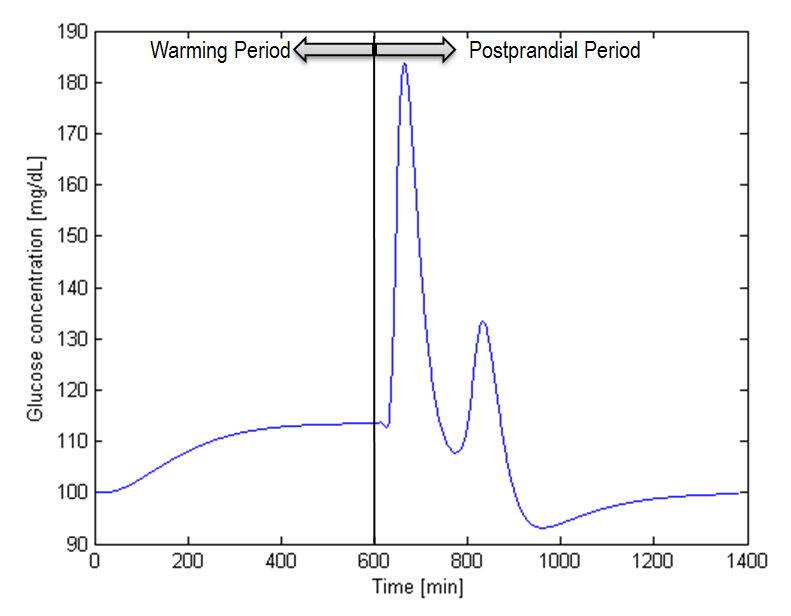
\epsfig{file=Figures/Bergmannobasal.png, width=0.8\textwidth}\caption{Bergman model simulation of a stop in the basal insulin infusion with nominal values of glucose effectiveness. Basal infusion is restored when the postprandial period begins.}
\label{fig:compare1}
\end{figure}

A small increase in glucose level can be seen as a consequence of the elimination of insulin infusion. Basal insulin removal causes a change in the settling point of the output variable, \textit{i.e.} glucose concentration. If basal insulin infusion stops in a model with smaller glucose effectiveness, the results are shown in Figure \ref{fig:compare2}.

\begin{figure}[hbtp]
\centering
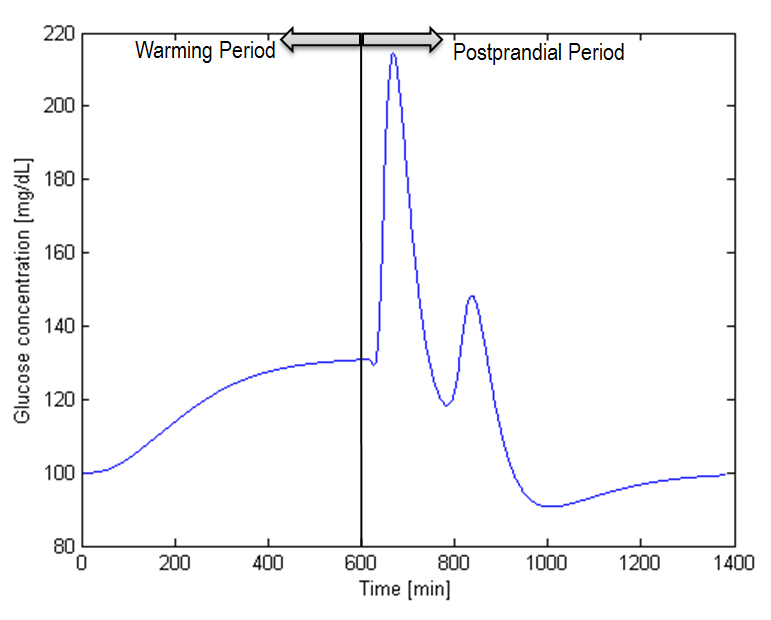
\epsfig{file=Figures/Bergmannobasal50percent.png, width=0.8\textwidth}\caption{Bergman model simulation of a stop in the basal insulin infusion with 50\% reduction in glucose effectiveness.}
\label{fig:compare2}
\end{figure}

The behavior observed in the ``warming'' period of Figures \ref{fig:compare1} and \ref{fig:compare2} is unrealistic. A diabetic patient whose insulin infusion is removed should become an unstable process, not just change its equilibrium point. Panunzi's model, in its equation (\eqref{eq:analysis2}) becomes a pure integrator if insulin is removed, making the system unstably increasing. Panunzi's model seems more suited to the physiology of glucose in diabetic patients in this case, but it also has its disadvantages. As it was said before, the Panunzi model represents the delay of insulin action in the equation of secretion, but that equation (\eqref{eq:Panunzi2}) is eliminated when simulating diabetic patients because of the absolute insulin deficiency in T1DM, so the delay effect is removed as well. If the delay is not reinstated somehow, the model simulates much faster dynamics when applying the bolus insulin in front of the simultaneous meal ingestion, making blood glucose to drop immediately after the injection, as can be seen in Figure \ref{fig:compare3}.

\begin{figure}[hbtp]
\centering
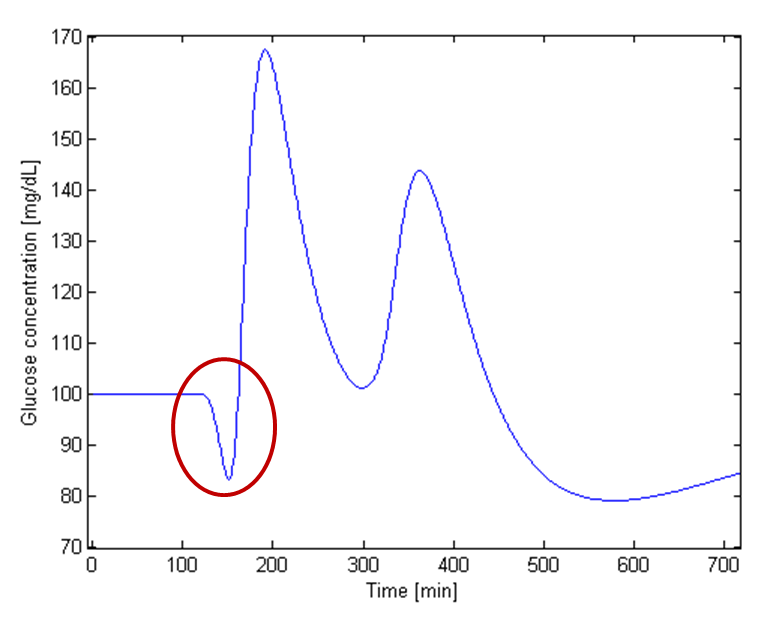
\epsfig{file=Figures/degaetano.png, width=0.8\textwidth}\caption{Panunzi model simulation of a postprandial period. Meal ingestion occurs at minute 120. Blood glucose drop after insulin bolus administration and before meal glucose appears into bloodstream is circled.}
\label{fig:compare3}
\end{figure}

This phenomenon is too pronounced and unrealistic. Even though insulin dynamics can, and often are, faster than gastrointestinal absorption, the effect on the displayed simulation is too abrupt and can yield to danger to the simulated patient. However, this effect can be easily avoided by adding a simple dynamic delay equation (\eqref{eq:analysis4}) to Panunzi's model, resulting in the next system of equations:
\begin{align}
  \dot{G}(t) &= -K_{xgl}X(t)G(t) +\frac{T_{gh}}{V_{g}} \label{eq:analysis3} \\
  \dot{X}(t) &= -k_{i}[X(t)-I(t)] \label{eq:analysis4}
\end{align}
With the addition of a new parameter to the model. This new parameter is not tuned and requires a nominal value to be set. This can be done simply by reviewing related literature. In \cite{helms2009insulin} Helms \& Kelley quantify the regular insulin action delay with a 30 minutes settling time. By looking at the new delay equation as a first order model, the time constant of the system can be calculated by assuming that the settling time is $3\times \tau$ (being $\tau$ the system's time constant), which reads a time constant of 10 minutes, and the parameter $k_{i}$ results to be equal to $0.1$ min$^{-1}$. The nominal parameter of this delay is dependent on the type of insulin being used, and it should be subject to deeper identification studies in the future. The response to a meal and a bolus in that case is shown in Figure \ref{fig:compare4}, where the dropping of glucose just after the bolus time is almost non present.

\begin{figure}[hbtp]
\centering
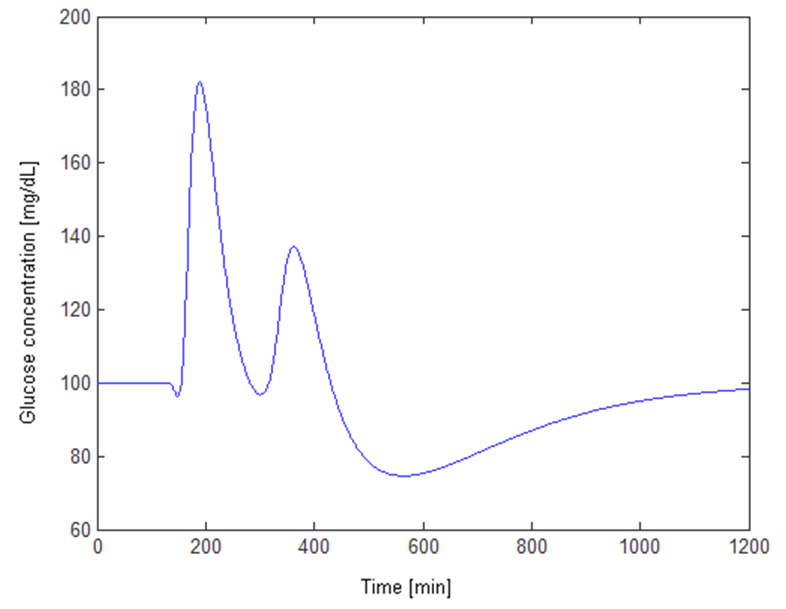
\epsfig{file=Figures/compare4.png, width=0.8\textwidth}\caption{Modified Panunzi model simulation of a postprandial period. Meal ingestion occurs at minute 120.}
\label{fig:compare4}
\end{figure}

The shown model is completely satisfactory for identification purposes and control. In order to check the model's reliability we look upon the work of 1994 by Torlone \textit{et al.} \cite{torlone1994}, where they showed a series of experiments in which insulin bolus is injected few minutes prior to an intravenous glucose infusion (infused in order to avoid hypoglycemia). This experiment shows clearly the effect and dynamics of insulin, and how it makes glucose to decrease in a similar way to an impulse response. From the work done by Torlone \textit{et al.} it can be extracted that there is no significant change in blood glucose until approximately 15 minutes after bolus injection, and then glucose drops steadily for 30 minutes until approximately 70 mg/dL (approximately 3 $mmol/l$). A very similar set-up was used for simulating the modification of Panunzi's model including insulin delay; an insulin bolus was applied and the effect on the blood glucose measured, as displayed in Figure \ref{fig:compare5}, but no intravenous glucose infusion was simulated.
%In Figure \ref{fig:perugia} insulin action is applied separately from any other action for almost one hour before the glucose infusion starts.

%\begin{figure}[hbtp]
%\centering
%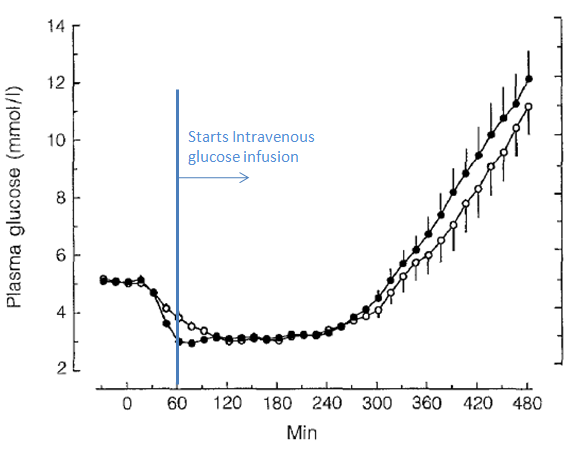
\epsfig{file=Figures/perugia.png, width=0.8\textwidth}\caption{Insulin impulse response of glucose after bolus and counteraction with intravenous glucose infusion \cite{torlone1994}. Black %dots represent the blood glucose measurements for monomeric insulin analog, and the white dots for human insulin.}
%\label{fig:perugia}
%\end{figure}

\begin{figure}[hbtp]
\centering
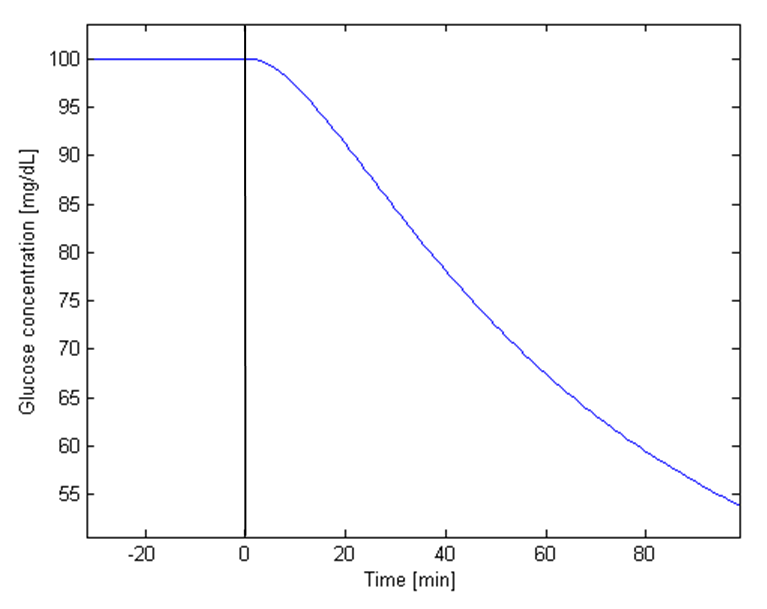
\epsfig{file=Figures/modifiedpanunzisimulation.png, width=0.8\textwidth}\caption{Variation of blood glucose (mg/dL) in Panunzi's model simulating a drop of glucose after insulin injection. Insulin is given at time $0$.}
\label{fig:compare5}
\end{figure}

In simulation, the response is exactly as expected: no significant change in blood glucose in the first minutes, and in the next half hour, glucose level drops to almost 70 mg/dL. This new dynamics make the new model much more reliable than Bergman or Panunzi's models in the referent to insulin simulation, and also proves valid the artificial delay added to the insulin action.

Another simple feature has also been included in the modified Panunzi model. Endogenous hepatic glucose production is one of the parameters of the model, $T_{gh}$, and it is considered constant. This parameter is actually variable, because endogenous hepatic production is suppressed by insulin. A simple variation of the model has been introduced, considering the $T_{gh}$ parameter to be reduced when plasma insulin surpassed a defined threshold, and defined as a piecewise function as follows:

\begin{equation} 
  T_{gh}=\left\{ \begin{array}{cc} 
  T_{gh0} & \mbox{ if } I(t) < T_{gh thr} \mbox{ }mIU/l\\ 
  K_{gh}\cdot T_{gh0} & \mbox{ otherwise } \\	
  \end{array} \right.
\label{eq:tegehache}
\end{equation}

where $T_{gh thr}$ is the above mentioned insulin threshold, $T_{gh0}$ is the basal endogenous production and $K_{gh}$ is the glucose production factor. 

With the described changes applied to Panunzi's model, a very useful yet simple model was developed and can be used for identification and identifiability studies in the following thesis. This resulting model will be mentioned in this thesis as ``Modified Panunzi Model'' 

 
		\chapter{Identification in Diabetes}
\label{sec:IdentificationInDiabetes}

%Incluir detalles de estudios realizados con datos en diabetes. Stahl, tesina, palerm, finan, etc

Insulin treatment is currently a necessity for T1DM patients. The insulin dose must be individualized foreach patient and for that physicians have traditionally characterized the patients using clinical parameters tuned heuristically. Such parameters represent an estimation of the insulin effect on glucose metabolism and the quality of glucose control depends on the performance of the parameters estimation. The latter is time consuming and requires constant patient reevaluation by a skilled health-care team. As a common consequence there is a mismatch between patient's needs and the actual insulin treatment, resulting in suboptimal glycaemic control.

In the artificial pancreas context the characterization of a patient is required to be much more accurate. Model individualization is required for every patient in order to get accurate enough predictions of the blood glucose levels. Using mathematical models for glucose prediction has been present in diabetes literature since the first models were published, but few satisfying results have been achieved for long term predictions. 

Patient identification deals with inter-patient (between patients) variability. The problem of characterizing inter-patient variability is handled individualizing models for each patient independelty. Intra-patient variability is much difficult to quantify, and in this thesis it is the main problem to overcome by the methodology and experimentation here described. From this point onward when referring to variability only intra-patient (within the patient) variability will be accounted. Intra-patient variability is the compound effect of several factors: not measured methabolism, stress intensity, hour of the day and meal uncertainty among others. The effects of this variability can be observed in many of the measured and identified parameters, often resulting in poor repeatibility in parameter identification.

In this chapter the most important and latest findings published in literature related to model individualization for diabetes will be reviewed.

\section{Patient Identification}
\label{sec:GlucoseCurveFitting} 

Glucose prediction from identification of models using experimental glucose data can be classified according to the nature of the model used. As described in the models in Section \ref{sec:ModelsForDiabetes}, models for diabetes can be data-driven or physiology-driven. 

From the engineering point of view, St{\aa}hl and Johansson published a pilot identification study \cite{stahl2009diabetes} using modified models from literature and data-driven models. This paper describes the experience of the first author, whom was diagnosed with diabetes shortly before the study, analyzing and modeling his own glucose profile over a period of several weeks. They analyzed in detail the characteristics of the data-set, including auto-correlation function, probabilistic distribution of the samples, sampling times, and statistical properties. They used models in literature for the input models, using in both cases (insulin and meal) two different pathways for fast and slow inputs. As for the endogenous models, they tested a battery of grey-box, data-driven models, including Auto Regressive models with exogenous inputs (ARX), Auto Regressive Moving Average models with exogenous inputs (ARMAX), General Transfer Function Models (GTFM), and state space models of increasing complexity. They used the models for validation of the identified patient under different prediction horizons. The study concluded that GTFM were well suited for prediction up to 2 hours ahead (8 simulation steps), but further horizons of prediction were not possible using any of the models used. 
%\begin{figure}[hbt]
%\centering
%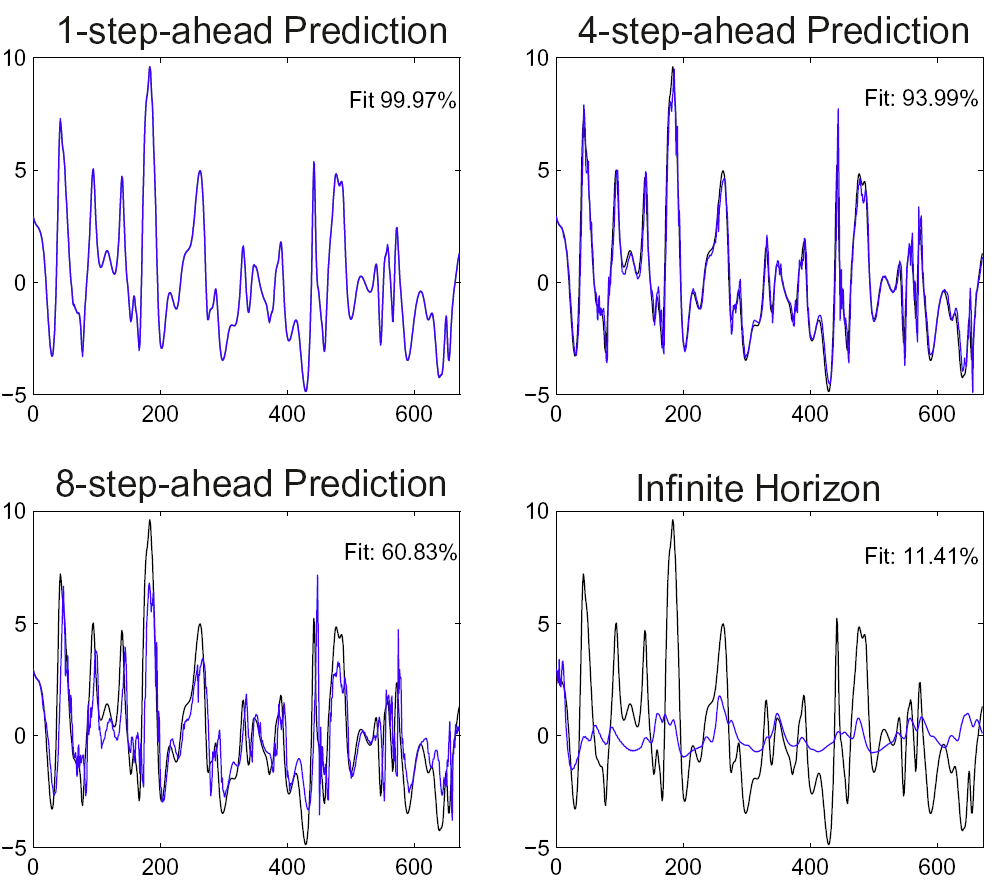
\epsfig{file=Figures/stahl.png, width=0.8\textwidth}\caption{Illustration of the degradation of predictive ability with the prediction horizon: upper left $\tau$ =1 (15 minutes); upper right $\tau$ =4 (1 hour); lower left $\tau$ =8 (2 hours); lower right $\tau =\infty$. Experimental data is plotted in black, and the predictions in blue.}
%\label{fig:stahl_compare}
%\end{figure}
The study performed by St{\aa}hl and Johansson was very useful in the diabetes identification scene as a pilot study, but it was nonetheless limited in many aspects. The data-set used was comprised only of data from one patient, thus neglecting completely the population variation in the diabetes metabolism. The study also only used self-measured capillary samples with irregular sampling times. Capillary blood glucose estimation can be subject to many errors and disturbances, and it is also too sparse to be able to capture glucose dynamics. More frequent sampling and more reliable measurements can improve the outcome of the study.

Johansson and his colleagues in Lund continued the investigation further on, publishing another study \cite{cescon2009subspace} where the effect of subspaced based models was considered. In this case, the data was taken from a patient that was wearing a CGM, monitored during three days under CSII (Continuous Subcutaneous Insulin Infusion) therapy, which provided with much more frequent data than in the previous study. Again, the models used for the inputs of the system where rather complex physiology-based models, like the UVA group meal model and the Cambridge insulin model described in chapters \ref{sec:ModelBasedOnDallaManEtAl} and \ref{sec:WillinskaEtAl} respectively. The rational behind this decision lies in the fact that the perturbations of the system (i.e. meals and insulin treatment) have an enormous impact on the diabetic patient glucose. The lack of physiologic insulin secretion in response to a meal make glucose homeostasis a hard task. In this context, insulin replacement in the subcutaneous tissue and meals represent a perturbation of the glucose system that needs a detailed description of the models used. This work showed that predictions with horizons larger than 30 minutes were very imprecise for CGM measurements. CGM involves more frequent sampling, but it introduces large errors in the measured blood glucose concentration, leading to great difficulties in the predictions. Nevertheless, this study introduces separation between meals and its related insulin dose and viceversa for easier identification, which is a concept that will be investigated later in this thesis.

Rollins \textit{et al.} published another self study, where a type 2 diabetic patient (Rollins himself) was monitored for several weeks \cite{rollins2010free} without insulin treatment. This study focused on predicting glucose by using many different measurements of the patients metabolism. The patient followed a normal life routine, wearing sensors of temperature, body activity, heat flux and CGM, as well as a diary with all relevant information about meals. They used data-driven models with multiple inputs in order to fit the patient's data. Model validation was performed against CGM estimations.
%\begin{figure}[hbtp]
%\centering
%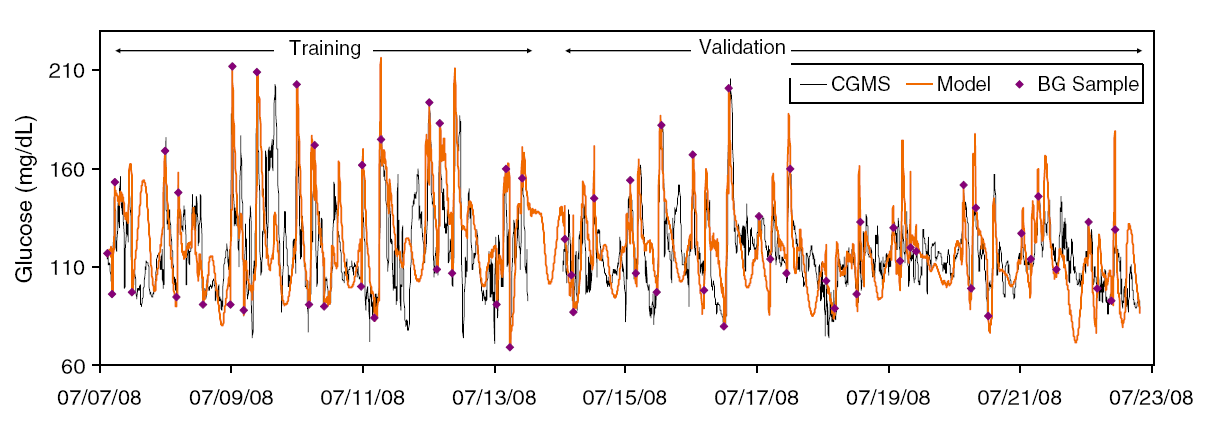
\epsfig{file=Figures/rollinsval.png, width=\textwidth}\caption{Model data fitting and validation of one of the models tested. Seven days were used for data fitting and 9 days for validation.}
%\label{fig:rollinsval}
%\end{figure}
Rollins showed that very good predictions ($r_{fit}$ up to 0.70) can be achieved if more data from the patient's metabolism and daily rhythm was provided. Unfortunately, these results are not extendable to type 1 diabetic patients since insulin treatments induce enormous perturbations to the system that were not modeled in this paper. Also, only 1 patient was monitored for this study, and diabetic patients may be reluctant to wear all the devices needed for full metabolic monitoring required for this study. Furthermore, complexity of this kind of monitoring make it unfeasible in clinical practice.

Georga \textit{et al.} studied the possibility of using a combination of physiological models as inputs to the system, and vector machine for regression as predictor of blood glucose \cite{georga2011glucose}. Their study comprised seven patients with 10 days average monitoring period. They incorporated the possibility of using an exercise model as an input to the glucose predictor. They showed results similar to those of \cite{rollins2010free}, but slightly less accurate predictions to those in \cite{stahl2009diabetes}, but comparisons between these studies are loosely sustained since the two previous studies only simulate one patient. No significant improvement was observed when including the exercise model into the prediction method.

In the work of Cameron \textit{et al.} on prediction of blood glucose for MPC controllers, a comparison of multiple models is performed \cite{cameron2012extended}. Four variations of a very simple data-driven model are tested for their predictive capabilities. The variations affect the meal prediction of the model in different ways, with increasing complexity:
\begin{itemize}
	\item No meal detection. Meals occur without announcement or reaction of the predictive model.
	\item Meal detection. Probabilistic detection of meals is implemented in the prediction model.
	\item Meal detection and anticipation. Meals are predicted and action is anticipated to the actual meal effect on glucose.
	\item Meal announcement. Meal time is assumed to be input by the user.
\end{itemize}
Prediction horizons of up to 5 hours are tested for all the variations of the model, both on simulated meal data and 19 days of experimental clinical data. Prediction capabilities are computed with mean error and root mean squared error (RMSE). Predictions are evaluated against prediction horizon on experimental data, and against time for a 2-hour prediction horizon in simulated meal data. This study presents large prediction errors (100 mg/dL) even for relatively short prediction horizon, but prediction performance increases as more information is estimated or provided to the model, being the meal announcement variation the most successful in terms of prediction capabilities.
%\begin{figure}[htb]
%\centering
%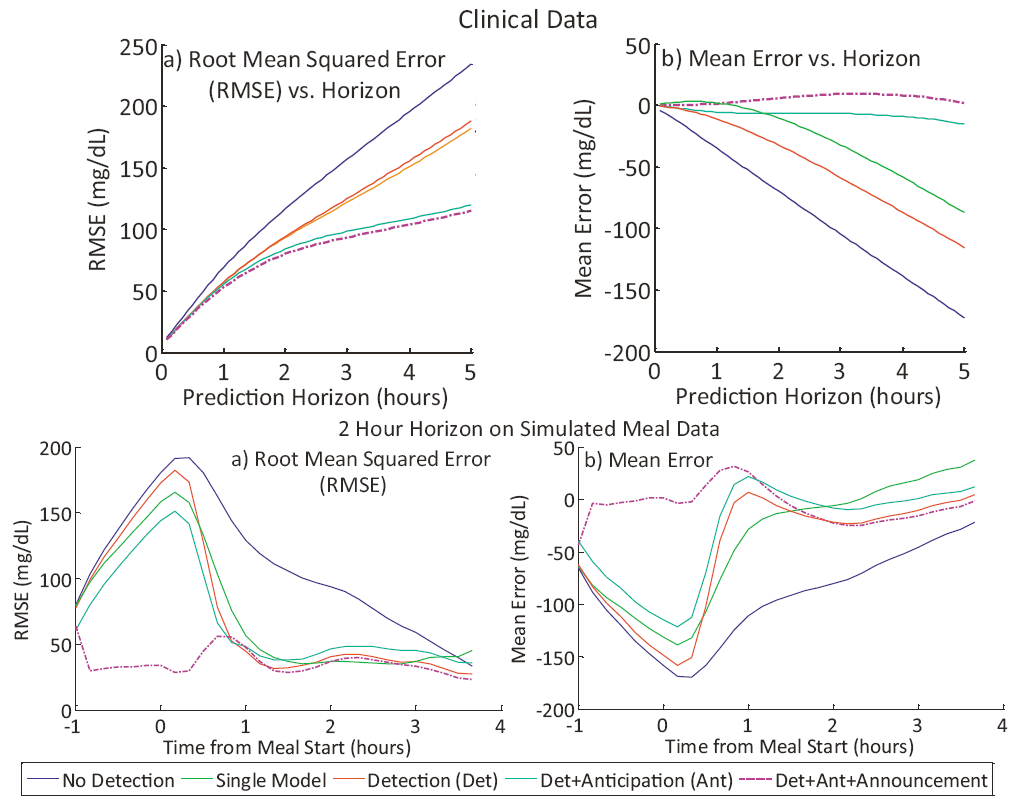
\epsfig{file=Figures/cameron_prediction.png, width=0.9\textwidth}\caption{Prediction results for all the variations of the model tested by Cameron \textit{et al.} Top panel presents the prediction error around mealtimes on simulated data. Bottom panel shows prediction error vs. prediction horizon across all 19 days of clinical data.}
%\label{fig:cameron_predict}
%\end{figure}

Palerm \textit{et al.} studied the possibility of using physiology models for identification of diabetic patients \cite{palerm2006robust}. They used a modification of the Cambridge model in data from five diabetic patients in a mixed meal response. The measurements were taken using a YSI 2300 STAT Plus\textsuperscript{TM} (YSI Inc., Yellow Springs, Ohio) very frequently (5 minutes period). This study incorporates an identifiability study of the Cambridge model's parameters, leading to a 4 parameter estimation for a well posed identification problem, at least locally. Given the non-linearities of the Cambridge model, global solvers ought to be used for the data fitting. In this case, Palerm \textit{et al.} used a hybrid method combining both global and local solvers to enhance identification speed \cite{rodriguez2006hybrid}. As opposed to the study performed by Johansson and his colleagues, in this case frequent reliable data was fitted, and several patients were individually identified and compared. Yet, validation results were not satisfactory.
%\begin{figure}[hbtp]
%\centering
%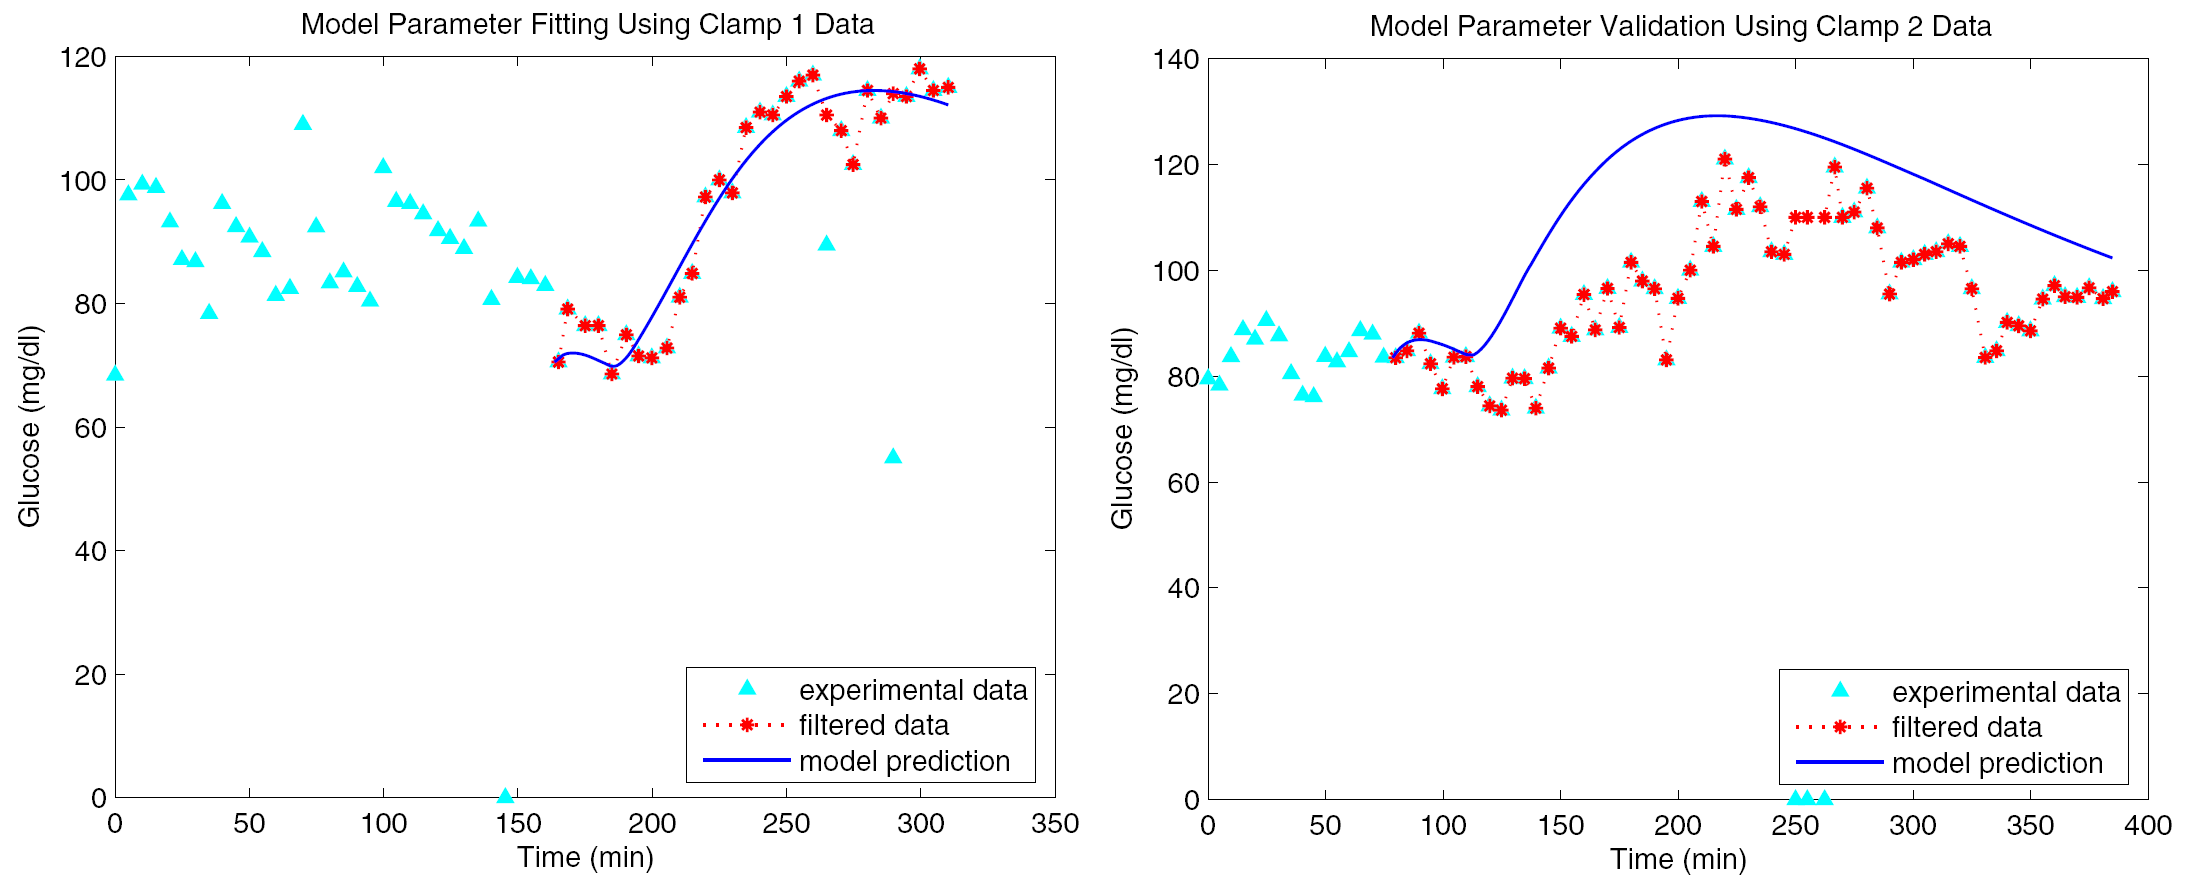
\epsfig{file=Figures/palerm_identification_composed.png, width=\textwidth}\caption{Model prediction versus data for one of the patients. Left graph shows the fitting of the data. Right graph shows the validation data on the same patient.}
%\label{fig:palerm_compare}
%\end{figure}

The work performed by Palerm \textit{et al.} supposed a solid first approach to the identification problem, but still, unsuccessful. The predictions were not able to mimic the response of the patients in different days, which can be caused either by model mismatch to the actual physiology or variations in the parameters within the same patient, or even maybe the incorrect use of data for identification.

Finan \textit{et al.} proposed a comparison of models identification for diabetic patients based on ARX models \cite{finan2009experimental}. They used data from 9 type 1 diabetic patients for identification comparing every prediction to that of a Zero Order Holder (ZOH). The ZOH predictions consisted simply in maintaining the glucose level for as long a the prediction horizon is. The predictions of the models were tested for prediction horizons of 30, 60 and 90 minutes. The study concluded that non significant improvement on the prediction capabilities (Relative Mean Square Error of the validation days) was observed from using ARX models instead of a ZOH. This conclusion is of great importance for identification in type 1 diabetic patients, since it discourages the use of pure data-based models in the prediction of glucose concentration. The authors conclude that non-modeled disturbances hinder greatly the performance of the selected models, and that getting reliable quantitative measures of exercise and stress levels would result in better quality predictions.
%Van heusden comparison \cite{van2011control}

Concerning the lack of identifiability showed so far by all of the available models in literature, Simone del Favero \textit{et al.} approached the identification problem from a completely new angle \cite{del2012glucose}. They proposed a method for identification using clinical index instead of purely mathematical quadratic indexes for data fitting. The clinical index consisted in a weighted index based on the glucose prediction danger to the patient. The reasoning behind this kind of fitting is that predictions for clinical patients are not worse as they differ from actual data, but as they unable to detect situations in which the patient may be endangered. For example in the case where a patient is heading towards hypoglycemia and the predictions are those of high glycaemic levels.

\section{Experiment Design for Artificial Pancreas}
\label{sec:ExperimentDesign}

Model identification is limited by both the model complexity and the amount and quality of the available data. The current state of models for identification has already been stated. In this chapter we will focus on the improvement of data acquisition techniques in the diabetes environment.

Predictions of the identified models are highly dependent on the identifiability of the model itself. Identifiability of a model is the facility to repeat an identification of its parameters under similar circumstances. Identifiability of a model is mainly dependent on the models structure, but it can also be improved by performing experiments that ease the process of the identification. The process of preparing data gathering experiments in order to enhance the identifiability of the model is called Optimal Experiment Design. Optimal Experiment Design is rare on the diabetes context due to the fact that data acquisition usually occurs in a clinical environment, where there are physical and ethical limitations to the experimental conditions.

There is a set of clinical tests that can help clinicians to either diagnose diabetes or to identify clinical parameters of glucose homeostasis:

\begin{itemize}
	\item \emph{Oral Glucose Tolerance Test (OGTT).} This standard test is used for diagnostics of diabetes. The test starts in the morning with the patient following the usual physical activity as in a normal day. The previous evening a meal of 30-50 g of carbohydrates is consumed. In the morning, a fasting blood sample is collected and then a solution of 75 g of glucose in water is drunk over a period of 5 minutes. Blood is then monitored afterwards at intervals. The most common interval though is a single sample (plus the fasting sample) 2 hours after the glucose solution ingest.
	\item \emph{Intravenous Glucose Tolerance Test (IVGTT).} This standard test is used for measuring the pancreas activity either in a healthy person or a diabetic patient. The glucose is administered in a antecubital vein over 60 seconds using a dose of 300 mg/kg. Glucose (and potentially insulin) is monitored starting at the moment of the infusion, with a fast sampling period (5 minutes or less) in the first period of the experiment, and more distanced measured at the end, lasting the whole of the experiment at least 3 hours.
	\item \emph{Postprandial Glucose Test.} This test is used to screen for diabetes and to evaluate treatments of therapies in diabetic subjects. The patient eats a balanced meal of measured components with a carbohydrate content of 100 g or more. The patient is then monitored for a minimum of two hours, and in case of necessity of testing a therapy, it is applied normally to the patient. This test is the easiest to perform since it follows the daily routine of the patients with a tight monitoring of blood glucose.
	\item \emph{Clamp Glucose Test.} Clamp tests are a battery of experiments that consist in artificially keeping blood glucose levels steady by intravenously infusing either glucose solution and/or insulin. They are difficult to perform as they require of an skilled doctor adjusting the glucose infusion levels to the appropriate concentration in order to lead blood glucose to the desired range. An example of clamp test is the euglycaemic hyperinsulinemic clamp, which consists on administering a large insulin infusion while maintaining glycemia in a controlled range of 90-100 mg/dL. This test permits the quantification of the insulin resistance of the patient without risking the patient to go to hypoglycemia.
\end{itemize}

Much more complex experiments can be performed for measuring metabolic fluxes in diabetic patients, as for example methods with radioactive tracers can help in the characterization of emptying rates in the digestive tract. In 2003 Basu \textit{et al.} described a triple-tracer method for assessing the postprandial glucose metabolism \cite{basu2003use}, which was later used by Dalla Man \textit{et al.} for developing a model of the gastrointestinal absorption of glucose \cite{man2007meal}. This type of tests though are extremely difficult to perform, even with single tracers; they require specialized instruments for the detection of the isotopes, and they are also much more intrusive to the patients involved

The field of optimal experiment design for diabetes has been developed greatly by Federico Galvanin and his team. In 2009 they published a design of a postprandial monitoring experiment with a variating insulin infusion throughout the post-prandial period \cite{galvanin2009}. The approach they used leads to results dependent on the model used, which for their case was the Cambridge model described earlier. They based their design on the optimality of 5 parameters of the endogenous glucose-insulin model, attempting to minimize the uncertainty in the identification of those parameters. After \textit{a priori} sensitivity analysis, they realized that two of the 5 parameters are highly correlated in the postprandial period and cannot be identified together so they reformulated the problem as the optimization of identifiability of 4 parameters, one of which was the ratio between the unidentifiable parameters. The outcome of the experiment design was a 2 meal monitoring where they tunned the CHO content of the meals and the insulin infusion from an insulin pump. The outcome of the experiment was relatively complex with the insulin infusion profile defined as a piecewise constant function with 12 levels and 11 level switching times.
%\begin{figure}[hbtp]
%\centering
%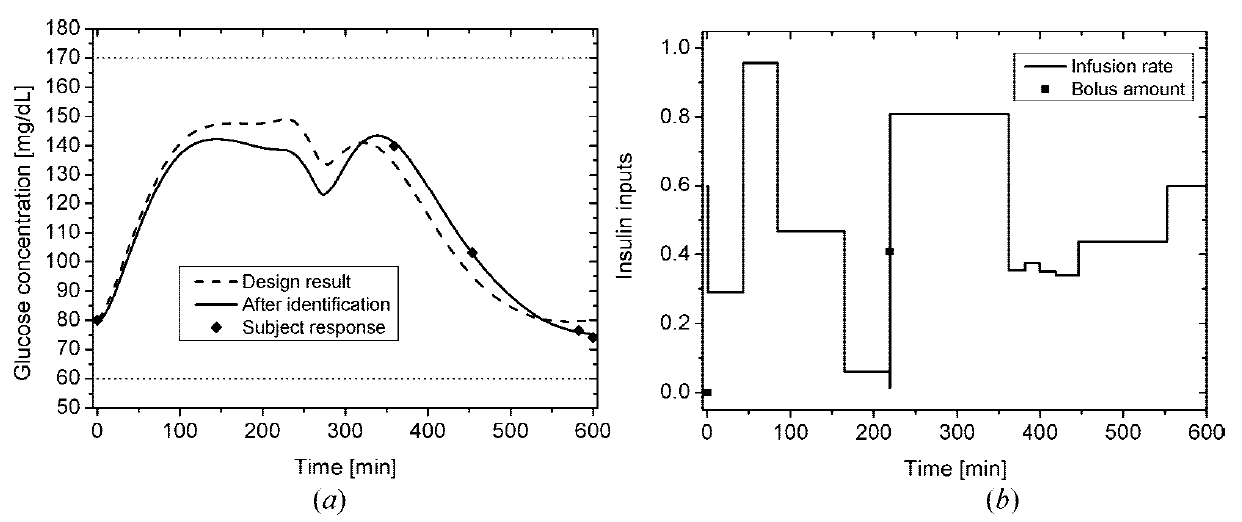
\epsfig{file=Figures/galvanininsulin.png, width=\textwidth}\caption{In the left panel the result of a simulation of the virtual patient is shown for the two meals period. In the right panel can be seen the piecewise function result of the experiment design for the insulin infusion.}
%\label{fig:galvanininsulin}
%\end{figure}

The qualitative result shown in the experiment design proposed by Galvanin \textit{et al.} is actually difficult to implement in a real experiment. Given that the models used are inaccurate, it is not advised to take the results of the experiment design accurately. Nevertheless, the results of this paper are very useful: it demonstrates that identifiability in diabetes is increased for longer experiments, and it shows that exciting the insulin input, statistically satisfactory parameter estimation can be achieved.

Later on, Galvanin \textit{et al.} published another work on optimal experiment design using on-line updates to the identifiability of the parameters \cite{galvanin2011optimal}. They realized from previous experimentation that model-based experiment design was too dependent on the model used. They decided to approach the issue in this paper introducing a model mismatch, based on the simple idea of simulating the data with one literature physiological model (in this case de UVA model) and identifying with another (the Cambridge model). The experiment design outcome is very similar to that of the previous work, with step shifts on the insulin infusion to the patient. %The new design is depicted in Figure \ref{fig:galvaninombre}.
%\begin{figure}[hbtp]
%\centering
%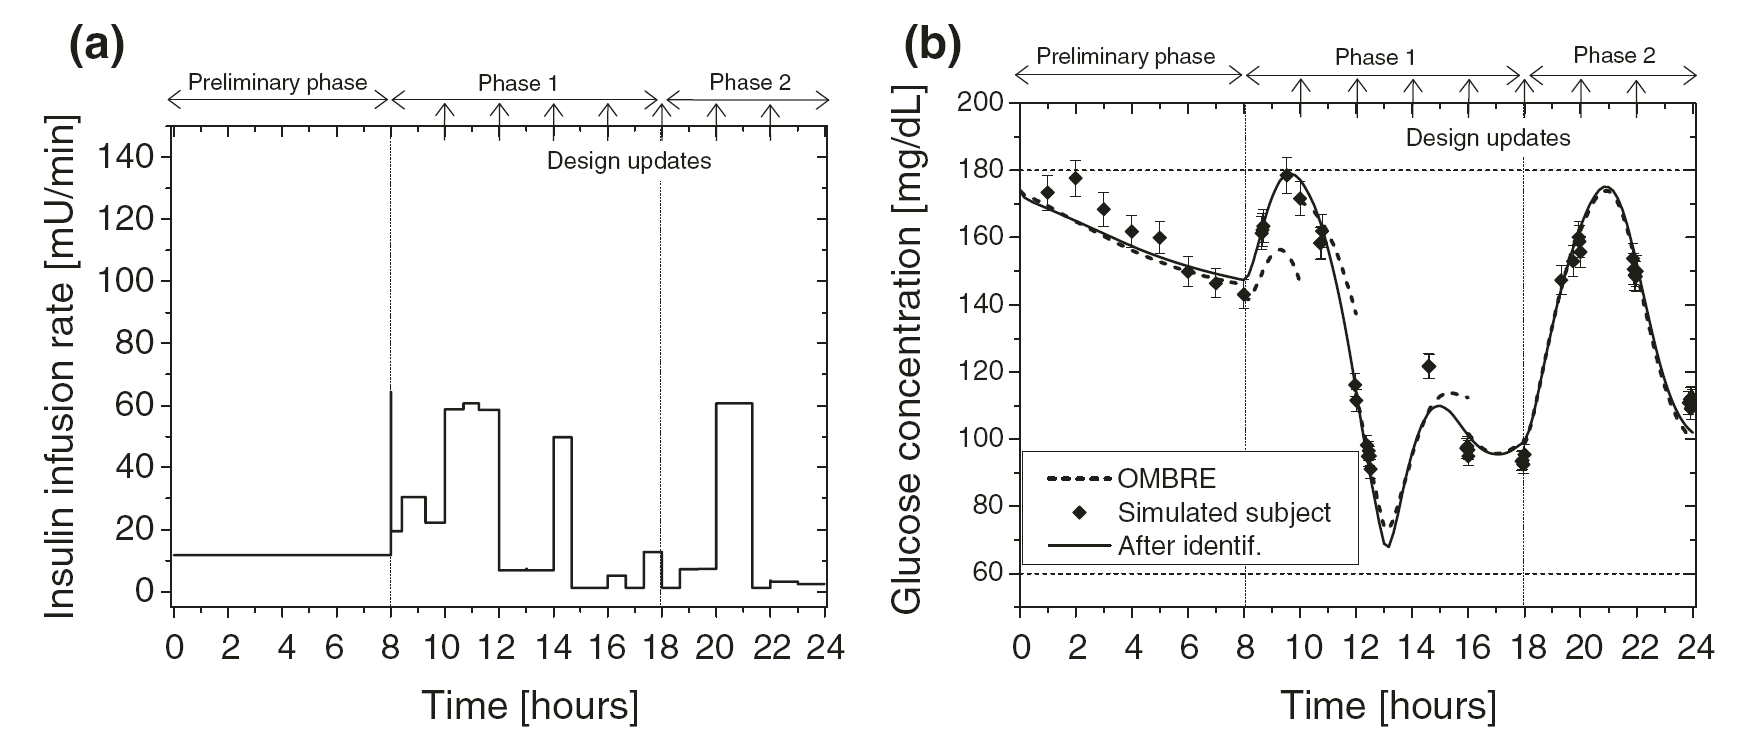
\epsfig{file=Figures/galvaninombre.png, width=\textwidth}\caption{In the (a) panel the insulin infusion is shown for the whole duration of the experiment. In the right panel the blood glucose concentration of the patient is displayed, including the identified model's predictions and simulations.}
%\label{fig:galvaninombre}
%\end{figure}

Galvanin \textit{et al.} concluded the study with a feasibility analysis of the experiments designed. When introducing the model mismatch, the classic model based experiment design was unable to provide feasible experiments. When using the on-line experiment redesign and identification, feasibility was achieved, and identifiability of the parameters was greatly improved. However, the amount of glucose and insulin to be delivered with the new method was much more aggressive. Clearly, this is unfeasible and unethical in the clinical setting as it would pose patients safety at risk.

Cobelli and Thomaseth published a study of optimal inputs for the Bergman minimal model using also optimality of identification of the parameters of the model \cite{cobelli1987minimal}. They focus on the design on finding optimal continuous functions of excitement to the endogenous model. They concluded that the outcomes of the experiment are very interesting from the modeling point of view, but of limited relevance in the diabetes context. Indeed, the optimal inputs obtained are too difficult to realize in clinical practice. They also imply that delayed insulin inputs can be useful for identification of certain parameters of the model.

Few other relevant works on the field of experiment design have been published. However, modifications on the traditional inputs with the aim of improving data quality is often seen in research of the artificial pancreas. Percival \textit{et al.} for example used delayed insulin bolus (2 hours after the meal) for the data acquisition of glucose profiles for a control algorithm \cite{percival}. %The scheme for the experiment monitoring and inputs can be seen in Figure \ref{fig:percival}
%\begin{figure}[hbtp]
%\centering
%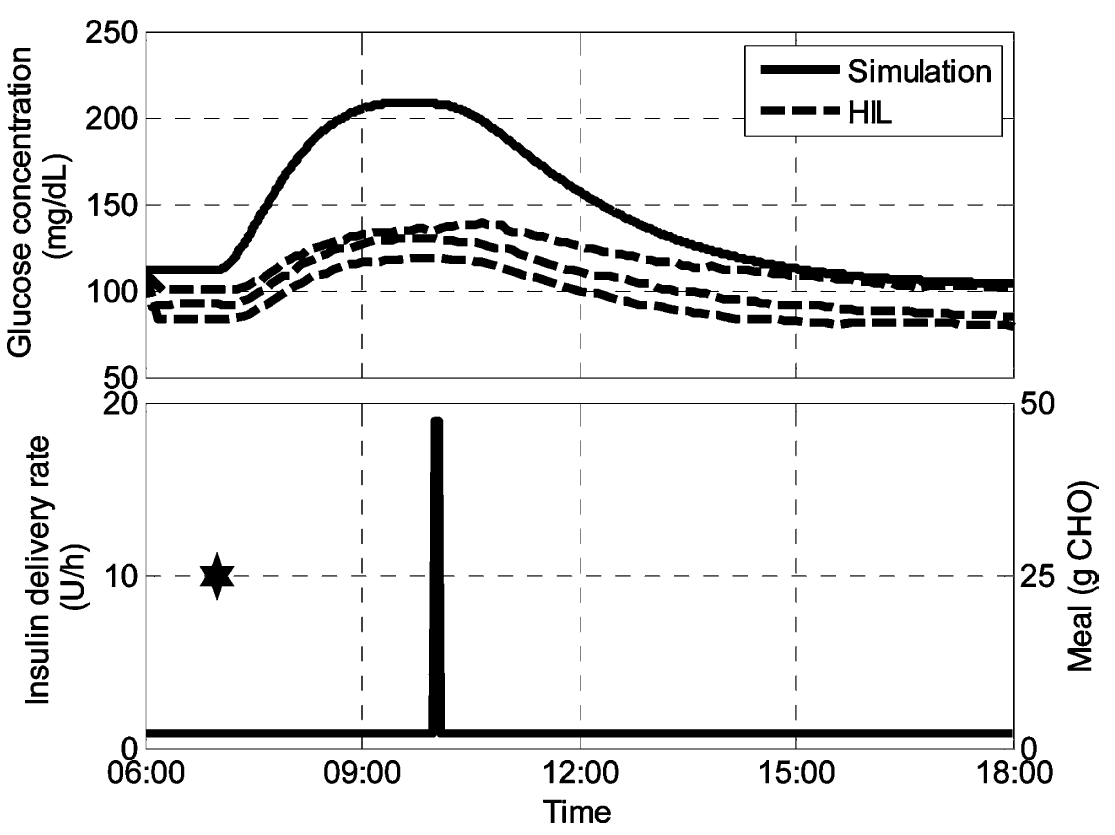
\epsfig{file=Figures/percivalshift.png, width=0.7\textwidth}\caption{Top panel shows the glucose simulation and CGM estimations for several calibration methods. Bottom panel corresponds to the inputs of the system for the same period. The star points at the meal ingestion time, and the impulse is the insulin bolus time.}
%\label{fig:percival}
%\end{figure}

Even though the clear objective of Percival \textit{et al.} when shifting the bolus time was to enhance the identifiability of the model, there is no further justification to it. In general, diabetes research lacks on simple experiments designed for the day-by-day routine of the diabetic patient; simple and safe enough experiments that will imply the patient participation and understanding of the disease he is living with, and the research related to it.

\section{Uncertainty and Interval Identification in Diabetes}
\label{sec:IntervalIdentificationInDiabetes}

Individualization of models for diabetes is greatly hindered by the fact that few models in literature consider intra-patient variability. In the models described in Section \ref{sec:ModelsForDiabetes} every model parameter stands for a physiological constant or function, and it is assumed to be characteristic to each patient. Most of the model proposed are published with some distribution in their parameters that resemble population values. These population values are an accepted quantification of the inter-patient variability for the parameters evaluated. However, characterization of a patient is dependent on the current metabolism of the patient, which is highly variable. This intra-patient variability has been regarded in literature with little detail.

One of the main sources of metabolic variability is the circadian rhythm of the patient. It is well established that the circadian variations of diabetic patients cause above average glucose levels in the early morning (event known as ``Dawn Phenomenon''), among other effects. The circadian effect has been quantified in the insulin dependance by Scheiner and Boyer \cite{scheiner2005characteristics}, showing a higher insulin relative dosage needed in the morning in type 1 diabetic patients. Higher insulin demand combined with constant basal infusion rates directly results in high morning glycemia, such as the reported in the Dawn Phenomenon. This work shows how insulin basal rate decreases for every age group after breakfast time, showing a periodic behavior of one of the better known physiologic parameters in diabetes: the insulin sensitivity. Furthermore, this work emphasizes the great difference in the population values when distributed by age groups, and suggests that a single probability distribution is not sufficient to characterize one parameter for the type 1 diabetic population.
%\begin{figure}[hbtp]
%\centering
%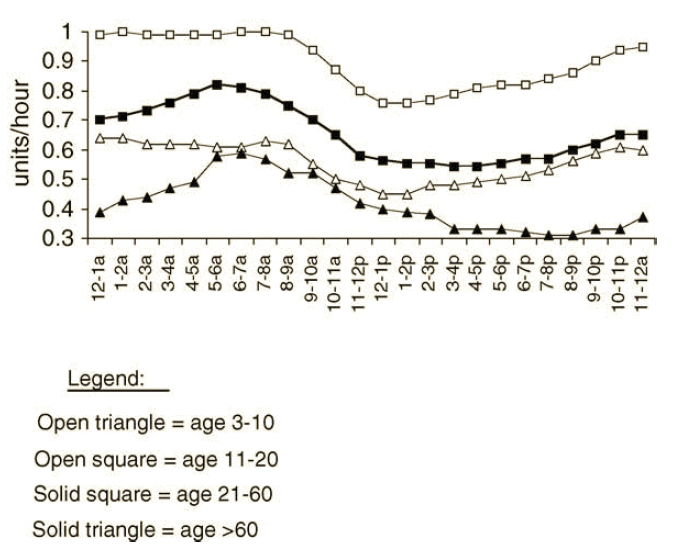
\epsfig{file=Figures/scheinercircadian.png, width=0.8\textwidth}\caption{Average hourly basal rate values by age group.}
%\label{fig:scheiner}
%\end{figure}

Understanding that physiologic parameters are not correctly characterized by only a number, several authors in recent years have been adapting physiological models in order to simulate patients with variability inherently considered. Using interval analysis methods and models is a new way of considering those parameters. Interval models consider internal parameters as ``ranges'' instead of punctual numbers. The parameter at a given time is actually unknown, but it is known to be comprised within the boundaries of the interval that defines it. The outputs of interval models are also intervals, and in the case of diabetes, the main output being glucose, means that we have to work with uncertain ranges of glucose.

Calm \textit{et al.} published work based on the Cambridge where modal interval analysis is applied for the plasma glucose prediction to face uncertain food intake and patient parameters such as insulin hepatic and peripheral sensitivity \cite{calm2007prediction}. The model was later validated against Monte Carlo simulations proving it to be a much more efficient in computation \cite{calm2010comparison}. The interval model developed was tested against several scenarios where parameters in the insulin absorption and meal absorption models were considered to have between a 10\% and 20\% variation. In general, wider variability considered in the parameters yield wider glucose outcomes. Calm \textit{et al.} showed that even relatively small variations considered in the parameters of the model (10\%) yield wide glucose prediction bands (approximately 100 mg/dL). Considering that sensitivity parameters of a real diabetic patient can be much more variable than the 10\% considered by this study, even larger glucose prediction bands are expected when characterizing diabetic patients in an experimental setting.
%\begin{figure}[ht]
%\centering
%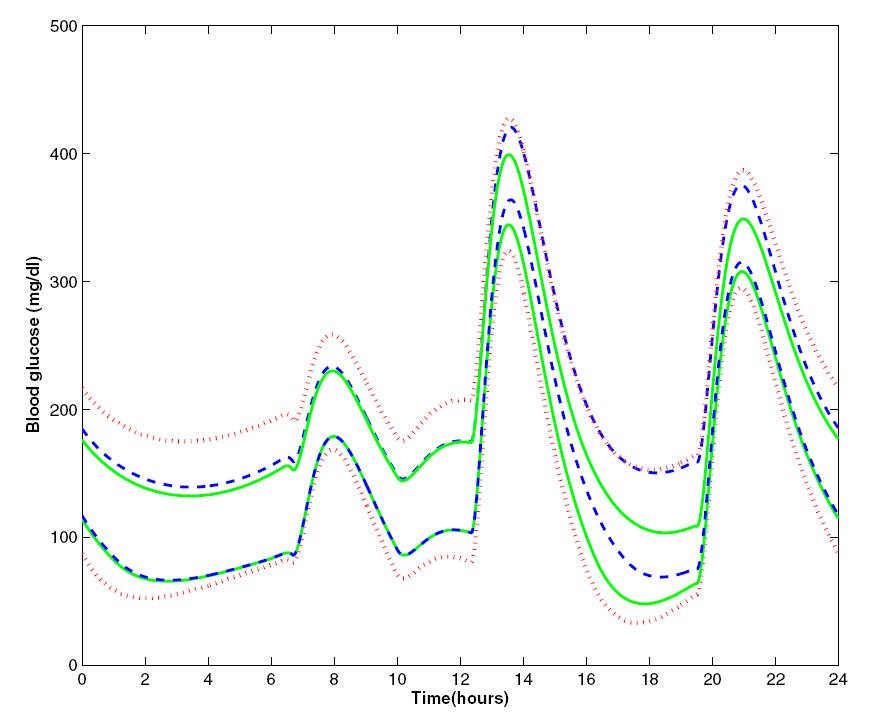
\epsfig{file=Figures/calmhovorka.png, width=0.9\textwidth}\caption{Envelopes obtained with the interval model for three different scenarios: 10\% variation in insulin sensitivity parameters (solid line), 20\% variation in insulin sensitivity parameters (dotted line) and 10\% variation with modified insulin bolus (dashed line).}
%\label{fig:calmhovorka}
%\end{figure}

Another approach to interval models simulation was undertaken by de Pereda \textit{et al.} on the Cambridge model \cite{de2012prediction}. They tackled the uncertainty analysis by using monotonicity analysis of the states of the model and its critical points. The bounds provided by this type of analysis are very similar to those proposed by Calm \textit{et al.}, but with the advantage of considering more parameters subject to uncertainty, as for example the insulin absorption lag time $t_{maxI}$. They also proposed the use of the uncertainty model as a short-term prediction tool, showing that for smaller prediction horizon scenarios, band widths do not grow excessively, and are suitable to use in regulation algorithms such as Model Predictive Control. The work done by de Pereda \textit{et al.} is very recent (2012), and it still has to be tested as a suitable method for identification and control.

To our knowledge, Kirchsteiger \textit{et al.} published the only identification procedure with consideration of uncertainty so far \cite{kirchsteiger2011estimating}. This work was initially based on a simple data-based transfer function model with 6 interval parameters. The identification was performed on data from 9 patients and three postprandial periods for each patient. After some trials, a simplified model structure was proposed for identification, due to identifiability issues, reducing it to only 4 interval parameters. The identification was posed as an optimization problem, where not only the fitting error was identified for 3 days, but also the standard deviation of each parameter considering the three postprandial periods. This procedure kept the parameters from resulting in too wide intervals, while still fitting the data of the patient. Even though the idea of identification of 3 separate days with common parameters is appealing, the study lacked of the proof of cross-validation on the data. Validation on single meals was performed, but not using the interval parameters, neither selecting a day \textit{a priori} as the validation day. It is unclear whether the day used for validation was just the 3rd day chronologically or the best case validation. Also, the data source on this study was treated without consideration of the possible errors introduced, which is a very important issue if not using glucose reference data.
%\begin{figure}[hbt]
%\centering
%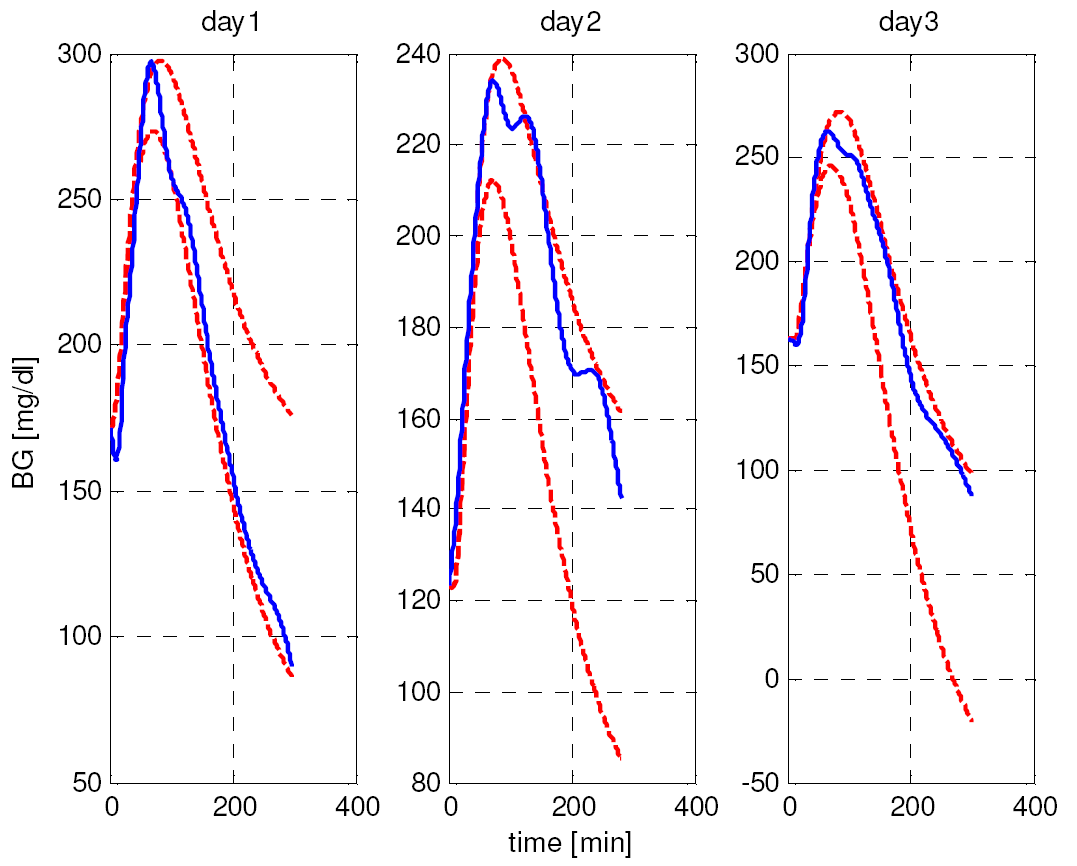
\epsfig{file=Figures/kirchsteiger.png, width=0.8\textwidth}\caption{Three-day identification of a diabetic patient's breakfasts. Blue solid line represents the spline-interpolated experimental glucose measurements. Red dashed lines are the upper and lower bounds given by the model.}
%\label{fig:kirchstegier}
%\end{figure}



 

		
\chapter*{Conclusions}
\label{sec:Conclusions}
\addcontentsline{toc}{chapter}{Conclusions}

Identification studies for type 1 diabetic patients are rarely found in literature. In this part of the thesis the most significant cases of patient individualization were reviewed, but unfortunately not one of them displays satisfactory prediction capabilities. In summary, individualization of type 1 diabetic models is still work in progress and special effort must be done in order to develop new strategies for predicting the glucose of a diabetic patient. A summary of the reviewed studies can be found in Table \ref{tab:iden_summary}.

\begin{sidewaystable}[hbtp]
	\centering
		\begin{tabular}{c|c|c|c}
		\emph{Reference} &	\emph{Model} & \emph{Achievements} & \emph{Drawbacks} \\
		\hline 
		\hline
		St{\aa}hl \textit{et al.} & \multirow{2}{*}{Data based model} & Real life measurements & \multirow{2}{*}{Data from only one individual} \\
		\cite{stahl2009diabetes} & & Up to 2 hour prediction & \\
		\hline 
		Cescon \textit{et al.} & \multirow{2}{*}{Data based model} & \multirow{2}{*}{Use of CGM} &Data from only one individual\\
		\cite{cescon2009subspace} & & & 30 minutes prediction \\
		\hline 
		Rollins \textit{et al.} & \multirow{2}{*}{Data based model} & Use of multiple sensors & Data from only one individual \\
		\cite{rollins2010free} & & Succesful fit $R=0.7$ & Absence of insulin disturbance \\
		\hline 
		Georga \textit{et al.}  & \multirow{2}{*}{Data based model} & \multirow{2}{*}{7 patients dataset} & \multirow{2}{*}{Poor predictions} \\
		\cite{georga2011glucose} & & & \\
		\hline 
		Cameron \textit{et al.}  & \multirow{2}{*}{Data based model} & \multirow{2}{*}{Experimental validation of the identifications} & \multirow{2}{*}{Poor predictions} \\
		\cite{cameron2012extended} & & & \\
		\hline 
		Palerm \textit{et al.} & \multirow{2}{*}{First principles} & Good data fitting & \multirow{2}{*}{Validation non satisfactory} \\
		\cite{palerm2006robust} & & Physiology based models &  \\
		\hline 
		Finan \textit{et al.} & \multirow{2}{*}{Data based model} & \multirow{2}{*}{Comparison against ZOH} & \multirow{2}{*}{No improvement over ZOH} \\
		\cite{finan2009experimental} & & & \\
	  \hline 
		Kirchsteiger \textit{et al.}  & \multirow{2}{*}{Data based model} & \multirow{2}{*}{Interval usage (uncertainty consideration)} & \multirow{2}{*}{No validation of the identifications presented} \\
		\cite{kirchsteiger2011estimating} & & & \\
	\end{tabular}
	\caption{Summary of identification studies.}
	\label{tab:iden_summary}
\end{sidewaystable}

Additionally, these studies have significant limitations as a few patients were included and validation of the identification was either not performed or poor. Only one study using physiology-based models presented validation data (Palerm \textit{et al.} 2006 \cite{palerm2006robust}), and even though validation data is presented, the results are not satisfactory. In that study, no consideration of uncertainty was performed. In this thesis a full cross-validation study on multiple patients is presented using first principles models. By adding uncertainty on the identification process, validation expected results will be improved in the whole population of patients examined.

Poor prediction and identification results published in literature suggest that individualization studies may be much more challenging for the diabetes paradigm than other classic engineering problems. These facts did not dissuade the author to advance as much as possible towards the solution of the identification problem, and in fact, new identification strategies are explored in this thesis that we believe strongly encourage the scientific community to push the limits of patient individualization forward. %esto puede ser motivation más que otra cosa, pero creo que queda bien aqui.

%The results of the master's thesis led to negative conclusions, so no publications were associated. Following this reasoning, and given that few identification studies in literature show validation data, and being patient individualization such an important matter, we can only assume that many groups have already tried to perform pilot identification studies with few success. We would like to encourage readers to scientifically acknowledge that non-successful studies, should be supported by a solid theoretical methodology, are as important for publication as successful experiments. I believe enormous efforts and resources are being spent in repeating experiments with negative results, not only in the diabetes context, and especially within the smaller research groups, because of negative results publication avoidance. %no se si lo escrito queda muy fuerte, pero me gustaría que un parrafo similar a este llegara a la tesis

Model accuracy is an open issue when dealing with glucose predictions. No proposed model of those reviewed in this thesis has shown exceeding performance over the others, and each one of them has been designed following a different set of directions. Models based on physiology are the most extended models in control and identification in diabetes, but they all lack on solid validation results. Model based experiment design can be used for a better use of the models proposed.

Almost no focus has been given to uncertainty consideration in the identification context in literature, despite the public knowledge of enormous variations in some of the physiology parameters, and large errors registered in continuous monitoring studies. Uncertainty treatment is key for better prediction of glucose concentration of diabetic patients, even using current models based in physiology. Interval models appear as the perfect choice for these type of problem, and will be used in this thesis to develop reliable identification methodologies. Of course, as modeling in diabetes advances, predictions can be more and more accurate, with less uncertainty from unmodelled dynamics to be considered by the intervals, but we consider this to be work to be done in parallel to the identification methodologies, which are the focus of this thesis.

Interval analysis and error-bounded estimation is a well established methodology, but have never been used in the diabetes context. This is most likely a consequence of the fact that estimating error incidence in glucose monitoring is usually very difficult. Sets of parameters that result from bounding all the possible errors in the glucose concentration space when measured by CGM are surely too large to be used in prediction studies and controller design. An interval approach more focused on the modeling of intra-patient variability is presented in this thesis, where the focus of the interval model is not to simulate all feasible responses to a single set of data but to bound several similar experiments on the same patient. With this repetition of days on the experiment, patient variability is expected to be present and interval models are expected to capture it. Coping with error in the measurement is handled by acknowledging a compromise between data fitting and measurement error. This type of interval bounding also focuses on the development of robust controllers because it provides not only patient characterization but also relative uncertainty measures for every different patient, which is closely related to robust controller design parameters.

 %breve resumen con el enfoque intervalar como solucion para todos nuestros problemas

		\part{Issues in Continuous Glucose Monitoring for Patient Identification}
		\label{sec:Issues}

		\chapter{Optimal Experiment Design}
\label{sec:OptimalDesign}

In the following chapter, a simple experiment is designed with the main objective of optimizing glucose data identifiability, regardless of the model used. Several safety measures have to be accounted for, including risk to hypo and hyperglycemia to the patient. The experiments are desired to be home-made, performed entirely by the patient, with few to non influence into the daily life of the patient.

\section{Introduction}
\label{sec:Introductionoptext}

Optimal experiment design requires of the designer to determine the experimental parameters to be used for optimization of identifiability. The diabetic patient model inputs are the variables that can be adjusted for the adequation of the experiment. For obtaining an optimal experiment, the best combination of the inputs regarding at the identifiability of the model is to be found.

Another variable usually considered in the optimization of the inputs is the sampling period of the measurements. In the experiments to be performed in this thesis, the measurements are considered to be sampled by a CGM, so the measurements are taken with the sampling period of the monitor (every 5 minutes), and the number of samples linearly increases with the experiment's length. The design problem is then transformed into how long the experiment should last. Usually, identifiability of the model increases with the number of samples because the experiment's data get richer, so the boundary of the experiment time is not of identifiability issues but of safety reasons. After medical consultation and examination of the resources for the experiments, it was decided that the length of the experiment was to be fixed at five hours after a meal, considering that most of the postprandial response and input excitation occurs in this period.

The most common inputs of a complete glucoregulatory model are two, the meals and the insulin infusion (supposing insulin pump treatment). Meals are usually considered as a disturbance, but in this work, mathematical models are used for simulating the meal absorption as an input to be designed. Insulin postprandial infusion is considered as an input as well. Both inputs can be parametrized as:
\begin{itemize}
	\item Parametrization of the meal system input:
\begin{enumerate}
	\item Meal size
	\item Meal composition
\end{enumerate}
	\item Parametrization of the insulin system input:
\begin{enumerate}
	\item Insulin bolus size
	\item Insulin bolus time (relative to meal time)
	\item Basal infusion rate
\end{enumerate}
\end{itemize}
Regarding meal composition, the published parameters in literature for the meal model analyzed in here, the UVA gastrointestinal model, were identified under the specific conditions listed below:
\begin{itemize}
	\item Caloric input: 10 kcal/kg
	\item Carbohydrate: 45\%
	\item Protein: 15\%
	\item Fat: 40\%
	\item Carbohydrate estimation and uncertainty: 90 $\pm$ 5 g
\end{itemize}
Carbohydrate estimation represents the size of the meal. The rest of the parameters determine the gastric emptying profile, and the identification performed in \cite{man2006system} produced the parameter values shown in Table \ref{tab:dallaman} based on the specified meal composition. Unfortunately, no identifications on different meal compositions have been performed on this model. Therefore, if optimum performance of the model is desired, experiments with this model are to be performed with similar composition to that shown in \cite{man2006system}. The size of the meal is  one of the parameters for the experiment design.

Regarding at the insulin input, the parameters chosen for optimization of the experiment design are much more complex than the those of the meal ingestion, which is only considered as an impulse. The insulin pump treatment can have any shape imaginable in accordance to the pump limitations. Designing an absolutely free insulin profile, i.e. a non-parametric input, would be too expensive in computational terms (for more information see \cite{walter1997}), so a parametric input is chosen. The classic profile of basal-bolus infusion is preserved in this experiment design for simplification purposes and to increase the patient's compliance with the experiment.

Once decided that a traditional treatment is going to be followed, the only parameters to be chosen for the experiment design are the amount of insulin to be given as a bolus, the basal insulin level, and the instant the bolus is administered. The basal rate was discarded from the parameter optimization set after a pilot experiment design. In this first experiment, the influence of basal was found to be neglectible on the model's identifiability when compared with the rest of parameters (meal and bolus). Also, adding a variable basal rate for each patient increased the number of optimization parameters too much, making the optimization much computationally intensive, which was not desired.

In summary, the experiment conditions to be tuned in the optimization are:
\begin{itemize}
\item $\tau$ - Delay of the insulin bolus with respect the meal time, in minutes. A positive delay means that the insulin dose is given after the meal and viceversa. The boundaries for the optimization problem are set to -60 and 300 minutes. Maximum advancement of the insulin bolus is defined so as to prevent hypoglycemic events.
\item Meal - The size of the meal in grams of carbohydrates. The boundaries for the optimization problem are 0 and 100 grams of carbohydrates.
\item Bolus - The amount of bolus insulin units to be given. The boundaries for the optimization problem are 0 and 10 insulin units. These boundaries were chosen using an insulin-to-carbohydrate ratio of 1:10 as population mean.
\end{itemize}
Only one meal per day is considered in order to avoid influences from the circadian variation of insulin sensitivity. The vector $\Xi$ (as seen in equation \eqref{eq:index}) is a vector of size $3\cdot n_d$, where $n_d$ is the number of days of monitoring. This vector is the output of the experiment design.

Given that the problem is highly non-linear (due to non-linearities of the index and the model) SSM global optimizer was used to obtain the solutions, as introduced in the Section \ref{sec:ScatterSearchForMatlab}. The constraints for the optimization problem are the restrictions of the blood glucose in order to keep the patient under safe health conditions. The simulation was forced to start from equilibrium in a blood glucose level of 100 mg/dL. The maximum level of glucose (hyperglycemic bound) was set to 250 mg/dL and the minimum level (hypoglycemic bound) was set to 70 mg/dL. These boundaries are respected at all times during the optimization of the experiment design.

Before the actual experiment design, a selection of the most relevant parameters is performed. A very simple analysis of identifiability is carried out on each of the models tested in order to discard non-relevant parameters that may induce optimality problems in the minimization of the experiment design. Repeated iterations of sensitivity analysis are done over the full model parameter set, iteratively removing any parameter that produces either singularity of the FIM or that presents a coefficient of variation larger that 30\%.

In the following lines results for experiment design in diabetes for two different models are shown. Despite the fact that Bergman's model has been proven unreliable for simulating some glucose dynamics, it is desirable to execute the experiment design methodology varying the models used in order to make the experiments as model-independent as possible. Therefore the first experiment design presented is calculated for this model. After that, experiments designed for the modified Panunzi model are displayed. Qualitative information can be extracted from every model's designed experiment. Common conclusions will be synthesized after the experiment design with both models considered and a feasible, patient-friendly protocol will be developed

\section{Experiments designed with Bergman's model}
\label{sec:ExperimentsDesignedWithBergmanSModel}

Initially, Bergman's endogenous model requires for the identification of three parameters, but two more are to be identified in a realistic identification experiment: distribution volume and basal glucose. Glucose distribution volume affects the glucose concentration with respect to the glucose inputs of the system throughout the postprandial period, and basal glucose states for the initial state of the glucose simulation, which for Bergman's model (equation \eqref{eq:Bergman3}) also affects the dynamics of the system. To complete the simulation of a diabetic patient, UVA's gastrointestinal model is implemented along with Cambridge's insulin absorption model. UVA's gastrointestinal model is one of the few models presented in literature with identification on mixed meals instead of glucose solution (even though the mixed meal used is far from being a classic meal), and that is the reason to choose it for the virtual patient's simulation. The Cambridge insulin absorption model was chosen based on the analysis of Willinska \textit{et al.} where it was compared against 11 literature models \cite{wilinska2005insulin} and showed excellent prediction capabilities. Bergman's endogenous model combined with UVA's glucose absorption model and Cambridge's insulin subcutaneous model sums up a total of 17 parameters, described in Table \ref{tab:bergmanparameters}.

%\begin{figure}[hbtp]
%\centering
%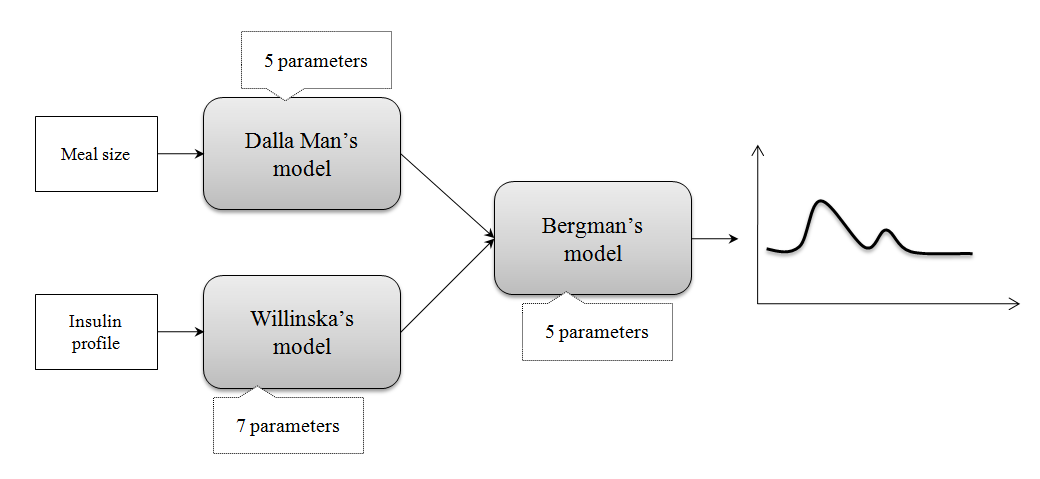
\epsfig{file=Figures/bergmanparameters.png, width=0.8\textwidth}\caption{Total number of parameters to be identified in Bergman's model}
%\label{fig:bergmanparameters}
%\end{figure}

\begin{table}[hbtp]
	\centering
	\begin{tabular}{| c | c | c | c |}
	\hline 
	Model	& Number & Parameter & Meaning \\
	\hline 
	Endogenous & 1 & $p_{1}$ & Glucose efficiency \\
	 & 2 & $p_{2}$ & Insulin action rate of disappearance\\
	 & 3 & $p_{3}$ & Insulin action rate of appearance \\
	 & 4 & $Vol_{g}$ & Distribution volume of glucose \\
	 & 5 & $G_{b}$ & Basal glucose \\
	\hline
	Gastric & 6 & $K_{abs}$ & Glucose absorption rate in the gut \\
	 & 7 & $K_{max}$ & Maximum gastric emptying \\
	 & 8 & $K_{min}$ & Minimum gastric emptying \\
	 & 9 & $b$ & Involved in the gastric emptying \\
	 & 10 & $c$ & Involved in the gastric emptying \\
	\hline
	Insulin & 11 & $V_{i}$ & Distribution volume of insulin \\
	 & 12 & $k$ & Proportion of insulin in the slow channel\\
	 & 13 & $k_{a1}$ & Transfer rate in the slow channel \\
	 & 14 & $k_{a2}$ & Transfer rate in the fast channel \\
	 & 15 & $k_{e}$ & Insulin elimination \\
	 & 16 & $V_{MAX,LD}$ & Michaelis-Menten parameter \\
	 & 17 & $k_{M,LD}$ & Michaelis-Menten parameter \\
	\hline
	\end{tabular}
\caption{Parameters integrated in Bergman's model.}
\label{tab:bergmanparameters}
\end{table}

Considering only blood glucose as the measurable output of the system, identifiability of all parameters is not expected. A three days experiment as the identification period was assumed. Later in this chapter, the choice of a three days experiment is discussed and proven to be adequate for the type of experiments being designed. A sensitivity analysis previous to the experiment design was performed, and the results are shown in Table \ref{tab:bergmanCV}. Only three iterations were needed to obtain a feasible set of parameters for identification on the Bergman model, but the algorithm initially discarded 8 parameters due to non-invertability of the FIM, which is closely related to structural non-identifiability. Indeed, the structural combination of Bergman model with the selected input models rendered many parameters difficult to identify just from glucose concentration data. Should richer data be available, such as plasma insulin data or tracer data of glucose flux from the gut, the sensitivity analysis would change.

\begin{table}[hbtp]
	\centering
	\begin{tabular}{ c | c | c | c | c }
	\multirow{2}{*}{Number} & \multirow{2}{*}{Parameter} & \multicolumn{3}{c}{Iteration} \\
	& & 1 & 2 & 3 \\
	\hline 
	1 & $p_{1}$ & - &	- &	- \\
	2 & $p_{2}$ & - &	- &	-\\
	3 & $p_{3}$ & - &	-	& - \\
	4 & $Vol_{g}$ & 0.25 & 0.14 & 0.13 \\
	5 & $G_{b}$ & 0.12 & 0.08 & 0.07 \\
	6 & $K_{abs}$ & - & - & - \\
	7 & $K_{max}$ & 0.25 & 0.24 & 0.23 \\
	8 & $K_{min}$ & 0.42 & - & - \\
	9 & $b$ & 0.16 & 0.12 & 0.04 \\
	10 & $c$ & 0.20 & 0.18 & 0.09 \\
	11 & $V_{i}$ & - & - & - \\
	12 & $k$ & 0.34 & 0.33 & - \\
  13 & $k_{a1}$ & 0.31 & 0.22 & 0.09 \\
	14 & $k_{a2}$ & - & - & - \\
	15 & $k_{e}$ & 0.22 & 0.14 & 0.12 \\
	16 & $V_{MAX,LD}$ & - & - & - \\
	17 & $k_{M,LD}$ & - & - & - \\
	\end{tabular}
\caption{Bergman's model parameter coefficient of variation (CV) for a three meals simulation. Each column represents an iteration in the sensitivity analysis. Parameters fixed to nominal values due to non-identifiability are indicated by a dash. Parameters fixed at iteration 1 are cause of structural non-identifiability.}
\label{tab:bergmanCV}
\end{table}

The final number of parameters identifiable, out of the initial 17, is 7. Only two of those parameters are part of the endogenous model, while three characterize the gastrointestinal model, and the other two are part of the insulin model, as can be seen in Figure \ref{fig:bergmanparametersidentifiable}.

\begin{figure}[hbtp]
\centering
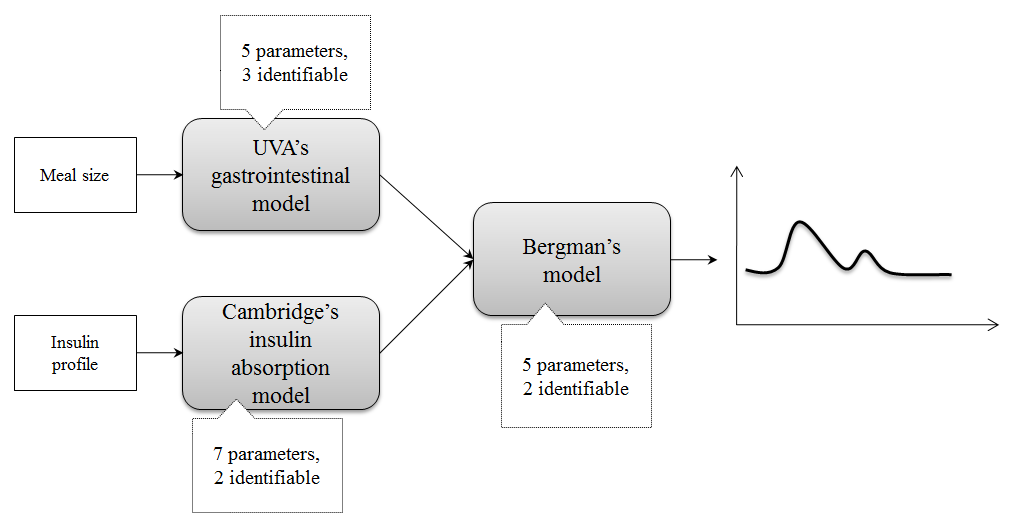
\epsfig{file=Figures/bergmanparametersidentifiable.png, width=\textwidth}\caption{Optimal set of parameters for Bergman's model combined with UVA's gastrointestinal model and Cambridge insulin absorption.}
\label{fig:bergmanparametersidentifiable}
\end{figure}

Those 7 parameters are used to optimally express the identifiability of the model. The experiments designed next expres the model's identifiability in the optimization index by using this optimal set of parameters. The range of days considered for experimentation is from one to four days. At the end of the experiment design for all the models under study, the best option was chosen from within of all the experiments designed, including the different options of parameter sets, models, and length of the experiments.

In the next lines, experiments designed comprising one, two, three and four days of monitoring are displayed. All experiments are designed using D-optimality, as described in Section \ref{sec:Optimizationofidentifiability}.

\begin{itemize}
\item{The results of an experiment designed for \textit{one} day of monitoring consisting on the five following hours to a meal are: $\tau = -31.59$ minutes, Meal $= 100$ g CHO and Bolus $=10$ IU. %is shown in Table \ref{tab:bergmanexperiment1day}.
%\begin{table}[hbtp]
%  \begin{center}
%	\begin{tabular}{| c | c | c |}
%	\hline 
%	Experiment & Units & Day 1 \\
%	\hline 
%	$\tau$ & minutes & -31,59 \\
%	Meal & gr CHO & 100 \\
%	Bolus & IU	& 10 \\
%	\hline	
%	\end{tabular}
%  \end{center}
%  \caption{Experiment conditions for the Bergman's model design considering one day of monitoring}
%	\label{tab:bergmanexperiment1day}
%\end{table}
In the case of only being able of monitoring one day, the optimum experiment to be followed requires the diabetic patient to advance the bolus approximately half hour, and then eat a large meal (100 grams CHO). It is worth remembering that 100 grams of carbohydrates is the top value given to the optimizer for the experiment design. Also, 10 is the top boundary for the bolus variable in the optimization, and it is the corresponding value of insulin for an standard treatment of insulin boluses for a 100 grams of carbohydrates meal. This means that, in addition to maximizing identifiability of the model, the experiment design keeps the patient under standard glycaemic control. This is a direct response to the output restrictions to the simulation model that force the patient's glucose to be within healthy range. The glucose profile associated to the experiment described can be seen in Figure \ref{fig:bergmanexperiment1day}.

\begin{figure}[hbtp]
\centering
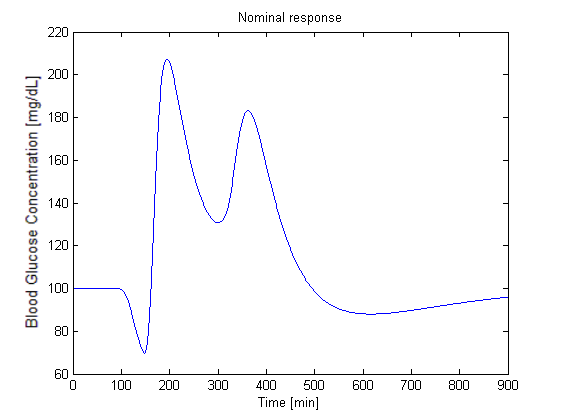
\epsfig{file=Figures/Berman_experiment_1day.png, width=0.9\textwidth}\caption{Bergman's model response to the proposed experiment for 1 day. Meal is ingested at time 120 min.}
\label{fig:bergmanexperiment1day}
\end{figure}

The glucose profile shows a very quick response to the advanced insulin bolus, dropping quickly to a level of approximately 70 mg/dL. This level is the safety threshold indicated as a constraint to the output in the optimization algorithm in order to keep the patient under safe conditions. This simulation shows how the optimizer is exciting the output variable as much as possible, and always keeping the (virtual) person safe.}

\item{The conditions of the experiment designed for \textit{two} days monitoring are:

\begin{itemize}
	\item Day 1. $\tau = 25.23$ minutes, Meal $= 86.81$ g CHO and Bolus $=10$ Insulin Units
	\item Day 2. $\tau = -29.58$ minutes, Meal $= 100$ g CHO and Bolus $=10$ Insulin Units
\end{itemize}

In this new experiment two different therapies are applied to the patient. The second day is a replicate of the conditions of the experiment design corresponding to only one day. In the first day of identification, a bolus of 10 insulin units is delayed approximately 25 minutes, for a meal of 86.81 grams of carbohydrates. In this case the proportion of insulin units to grams of carbohydrates of the meal is not maintained, thus, not a standard glycaemic control is performed on the patient (including the effect of the delay). The glucose profile for the designed two-day experiment is shown in Figure \ref{fig:bergmanexperiment2day}.

\begin{figure}[hbtp]
\centering
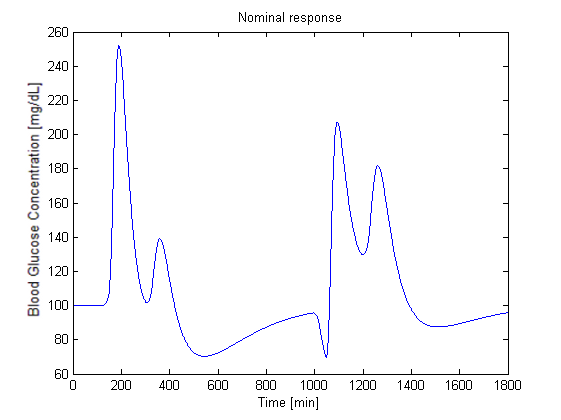
\epsfig{file=Figures/Berman_experiment_2day.png, width=0.9\textwidth}\caption{Bergman's model response to the proposed experiment for 2 days. Meals are ingested at time 120 and 1020 min.}
\label{fig:bergmanexperiment2day}
\end{figure}

Observing the first day response of the model to the proposed experiment, the fact of non-proportionality of insulin to carbohydrates makes more sense. The model moves from 250 mg/dL down to 70 mg/dL, which are the top and bottom safety thresholds in the experiment design optimization algorithm. The optimizer is exciting the measurable variable (blood glucose) through all the feasibility glucose range in order to maximize identifiability. Given that in the first day, due to the delay of the insulin bolus, there is no falling of the blood glucose to the lowest level, it has to drop to that level after the meal, that is why the insulin bolus is still relatively big with respect to the size of the meal. Given those values, the maximum amount of carbohydrates for that meal, so that the experiment does not exceed the upper safety threshold, is $86.81$.

It is interesting to understand why the two days differ in the relative bolus administration time. In the first day, no insulin excitation is applied in approximately 30 minutes from meal time and all the information extracted from that period is contributing to increase the identifiability of the gastrointestinal input model, the UVA model. In the other day, the opposite situation is happening: only the insulin subcutaneous model is experimenting excitation in the first period of the simulation, so information from glucose is affecting only the parameters of that model. The strongest the variation of the states of the model in that period, the greater the identifiability will be.}

\item{The conditions of the experiment designed for \textit{three} days monitoring are:
\begin{itemize}
	\item Day 1. $\tau = 26.43$ minutes, Meal $= 85.6$ g CHO and Bolus $=10$ Insulin Units
	\item Day 2. $\tau = -30.44$ minutes, Meal $= 100$ g CHO and Bolus $=10$ Insulin Units
	\item Day 3. $\tau = -30.71$ minutes, Meal $= 100$ g CHO and Bolus $=10$ Insulin Units
\end{itemize}

In this case, the advancing of the bolus is repeated two days. Given that the meals do not have to be consecutive, or that one day does not have any relation to the others, the order of the experiment days is not relevant for the result of the experiment. The glucose profile for the designed three-day experiment is shown in Figure \ref{fig:bergmanexperiment3day}.

\begin{figure}[hbt]
\centering
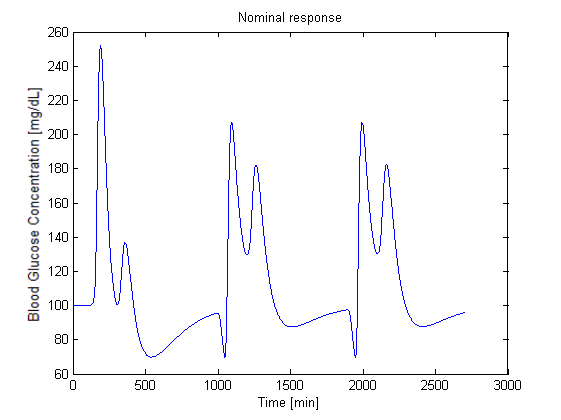
\epsfig{file=Figures/Berman_experiment_3day.png, width=0.9\textwidth}\caption{Bergman's model response to the proposed experiment for 3 days. Meals are ingested at time 120, 1020 and 1920 min.}
\label{fig:bergmanexperiment3day}
\end{figure}

The second and third days are virtually the same experiment, and the first day displays again the extreme excitation of glucose between safety boundaries. It can be appreciated once again how there is a separation of dynamics between the different input models.}

\item{The conditions of the experiment designed for \textit{four} days monitoring are:
\begin{itemize}
	\item Day 1. $\tau = 25.44$ minutes, Meal $= 86.81$ g CHO and Bolus $=10$ Insulin Units
	\item Day 2. $\tau = 14.36$ minutes, Meal $= 99.64$ g CHO and Bolus $=10$ Insulin Units
	\item Day 3. $\tau = -29.92$ minutes, Meal $= 100$ g CHO and Bolus $=10$ Insulin Units
	\item Day 4. $\tau = -30.88$ minutes, Meal $= 100$ g CHO and Bolus $=10$ Insulin Units
\end{itemize}

In this final case the two last days are repeated again, displaying an advance of the insulin bolus, and a new delayed bolus profile appears, but in this case with a big meal. The delay on the bolus is smaller so that the meal can be bigger, contributing to the improvement of identifiability of UVA's gastrointestinal model. The glucose profile for the designed four-days experiment is shown in Figure \ref{fig:bergmanexperiment4day}.

\begin{figure}[hbt]
\centering
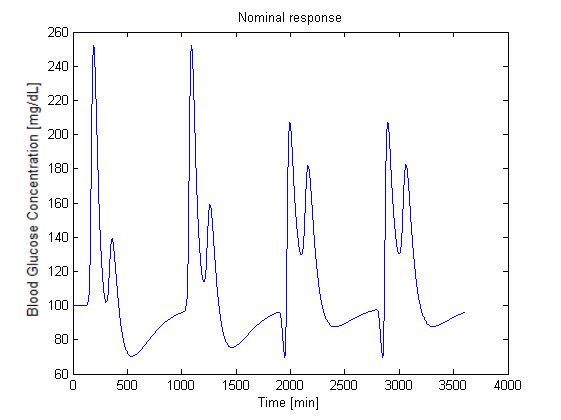
\epsfig{file=Figures/Berman_experiment_4day.png, width=0.9\textwidth}\caption{Bergman's model response to the proposed experiment for 4 days. Meals are ingested at time 120, 1020, 1920 and 2820 min.}
\label{fig:bergmanexperiment4day}
\end{figure}

As it can be observed, there is not much difference in the first two days of identification because the difference in the meal size is relatively small.}
\end{itemize}

The most relevant observation of this experiment design with the Bergman model is that separating dynamics of the input models is the key to improve the identification of the whole system. It is better for a model general identifiability to advance the bolus rather than having it delayed following the cases of one day experiment design (advancing bolus) and three-day experiment design (advancing bolus two days out of three). However, a better scenario comprises both situations, advancing and delaying the bolus. A minimum of a two-day experiment is then required for basic identification of the system. 

Experiment's length is selected attending to: 1) identifiability conditions, 2) experiment parameters and 3) practical implementation aspects. It has been stated that a minimum of two days for monitoring seems reasonable for identification purposes due to the two different profiles of experiment. Naturally, as more data (more days of experiment) is available, the probability of a satisfactory identification increases. However, the practical implementation aspect limits the number of days in a experiment. In Figure \ref{fig:Bergmandays} evolution of identifiability of each parameter of the optimal set in Bergman's model can be observed for all the cases exposed before and after the experiment design.

\begin{figure}[hbtp]
\centering
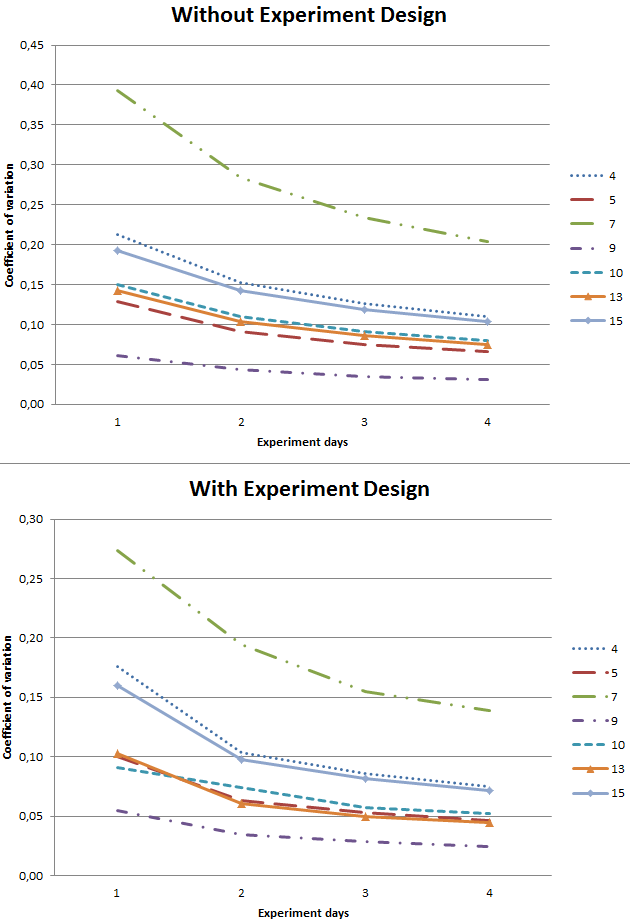
\epsfig{file=Figures/Bergmandays.png, width=0.8\textwidth}\caption{Coefficient of variation for Bergman's model's parameters. Top graph shows the evolution of the parameters' identifiability with experiment length. Bottom panel displays the identifiability of the same parameters applying the designed experiments. It is clearly shown how identifiability increases (CVs decrease) with experiment length. Parameter numeration is equivalent to that of Table \ref{tab:bergmanCV}.}
\label{fig:Bergmandays}
\end{figure}

An abrupt decrease in the coefficient of variation of all parameters occurs between one and two days of monitoring, reinforcing the mentioned minimum of identifiability in two days, both for the experiments with and without optimal design. If more days are added to the experiment identifiability keeps increasing less rapidly. Very similar trends in the identifiability rise are observed for both the original experiments and for the optimal designed experiments. The identifiability levels, as measured by coefficient of variation of the parameters are much lower for any experiment length when choosing the optimal design for the experiment. A three-day experiment was chosen thinking on the limitations introduced by the clinical implementation of the experiment. It is desired to have as many identification days as validation days, which makes the real monitoring period twice as long as the experiment designed. Given that the average sensor lifetime in a continuous glucose monitor is approximately one week, the three days experiment was chosen as monitoring duration, for maximization of identifiability. Results have to be compared with designed experiments based on other models in order to make the experiments as model-independent as possible. Comparison between the coefficients of variation of a three-day identification experiment is displayed in Figure \ref{fig:Bergmanoptdesign3days}.

\begin{figure}[hbt]
\centering
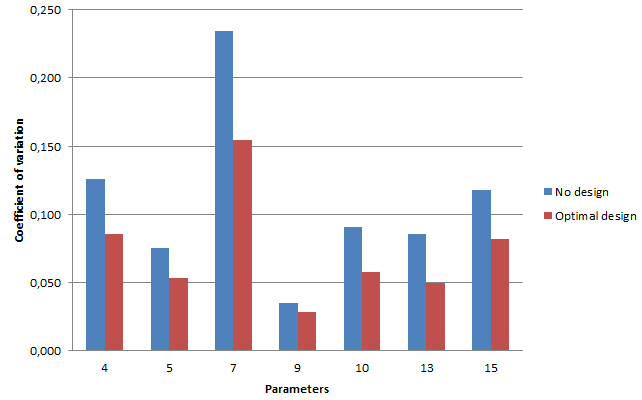
\epsfig{file=Figures/Bergmanoptdesign3days.png, width=\textwidth}\caption{A comparison of identifiability for each parameter with and without the experiment design for the case of a three meals monitoring.}
\label{fig:Bergmanoptdesign3days}
\end{figure}

A remarkable fall in the coefficient of variation is observed for all the parameters, and not just for the general identifiability of the model. In the original sensitivity analysis of Bergman's model all the parameters were selected to be identifiable, assuming identifiability of the model when all its parameters presented CVs below 30\%. For Bergman's model the limitant parameter (highest CV) was parameter 7, $K_{max}$. Using experiment design we reduce the variability of this parameter to half of the identifiability threshold, not sacrificing identifiability in any of the other parameters.

\section{Experiments designed with modified Panunzi's model}
\label{sec:ExperimentsDesignedWithPanunziSModelModified}

Identifiability of the modified version of Panunzi's endogenous model, which was described in Section \ref{sec:CriticalSelectionOfModels} will be analyzed next. Modified Panunzi's model and the two input models already used for Bergman's system comprise a total of 16 parameters, 4 of which correspond to the endogenous model. The 16 parameters are described in Table \ref{tab:panunziparameters}.

\begin{table}[hbt]
  \begin{center}
	\begin{tabular}{| c | c | c | c |}
	\hline 
	Model	& Number & Parameter & Meaning \\
	\hline 
	Endogenous & 1 & $K_{xgl}$ & Insulin sensitivity \\
	 & 2 & $V_{g}$ & Distribution volume of glucose\\
	 & 3 & $T_{gh}$ & Hepatic balance \\
	 & 4 & $k_{i}$ & Insulin action delay \\
	\hline
	Gastric & 5 & $K_{abs}$ & Glucose absorption rate in the gut \\
	 & 6 & $K_{max}$ & Maximum gastric emptying rate \\
	 & 7 & $K_{min}$ & Minimum gastric emptying rate \\	
	 & 8 & $b$ & Involved in the gastric emptying \\
	 & 9 & $c$ & Involved in the gastric emptying \\
	\hline
	Insulin & 10 & $V_{i}$ & Distribution volume of insulin \\
	 & 11 & $k$ & Proportion of insulin in the slow channel \\
	 & 12 & $k_{a1}$ & Transfer rate in the slow channel \\
	 & 13 & $k_{a2}$ & Transfer rate in the fast channel \\
	 & 14 & $k_{e}$ & Insulin elimination \\
	 & 15 & $V_{MAX,LD}$ & Michaelis-Menten parameter \\
	 & 16 & $k_{M,LD}$ & Michaelis-Menten parameter \\
	\hline	
	\end{tabular}
  \end{center}
  \caption{Parameters to be identified in Modified Panunzi's model.}
	\label{tab:panunziparameters}
\end{table}

Many of the parameters involved in the sensitivity analysis for Bergman's endogenous model are repeated for this case, but the numeration is different due to the different number of parameters in the endogenous model. The results of the identifiability study are shown in Table \ref{tab:panunziCV}.

\begin{table}[hbt]
	\centering
	\begin{tabular}{ c | c | c | c | c | c | c }
	\multirow{2}{*}{Number} & \multirow{2}{*}{Parameter} & \multicolumn{5}{c}{Iteration} \\
	& & 1 & 2 & 3 & 4 & 5 \\
	\hline 
	1 & $K_{xgl}$ & 1.14 & 0.98 & 0.55 & 0.53 & 0.31\\
	2 & $V_{g}$ & 0.46 & 0.43 & 0.26 & 0.24 & 0.23\\
	3 & $T_{gh}$ & 0.51 & 0.18 & 0.18 & 0.18 & 0.06\\
	4 & $k_{i}$ & 4.91 & - & - & - & -\\
	5 & $K_{abs}$ & 1.60 & 1.12 & 0.67 & - & -\\
	6 & $K_{max}$ & 0.78 & 0.66 & 0.53 & 0.24 & 0.24\\
	7 & $K_{min}$ & 0.87 & 0.68 & 0.33 & 0.33 & 0.30\\	
	8 & $b$ & 0.41 & 0.20 & 0.18 & 0.17 & 0.13\\
	9 & $c$ & 0.66 & 0.51 & 0.34 & 0.20 & 0.18\\
	10 & $V_i$ & - & - & - & - & -\\
	11 & $k$ & 0.91 & 0.81 & 0.36 & 0.29 & 0.27\\
	12 & $k_{a1}$ & 0.45 & 0.43 & 0.26 & 0.25 & 0.20\\
	13 & $k_{a2}$ & 3.77 & 2.57 & - & - & -\\
	14 & $k_{e}$ & 0.88 & 0.71 & 0.49 & 0.49 & 0.30\\
	15 & $V_{MAX,LD}$ & 1.92 & 0.92 & 0.66 & 0.62 & -\\
	16 & $k_{M,LD}$ & - & - & - & - & -\\	
	\end{tabular}
\caption{Modified Panunzi's model parameter coefficients of variation (CV) for a three meals identification.}
\label{tab:panunziCV}
\end{table}

Following the same methodology than in the Bergman's model analysis, only two parameters were not identifiable because of FIM singularity. These two parameters (10 and 16) show in Table \ref{tab:panunziCV} with their row in the first iteration blank. Parameter 16 is fixed in the identification because of its low sensitivity, and parameter 10 is fixed to its nominal value due to a very strong correlation (proportional relation) to parameter 1. Five iterations on the sensitivity analysis were needed for the modified Panunzi's model in order to obtain a feasible set of parameters for identification, to produce a 10 parameter set with good identifiability.

The set of parameters in the last column of Table \ref{tab:panunziCV} is considered the optimum set of parameters for identification even though 3 of the parameters of that set present CVs in the acceptable limit of identifiability (30\%). Those parameters ($K_{xgl}$, $K_{min}$ and $k_{e}$) in the proposed limit of identifiability are considered of great importance for the identification of individual patients in the postprandial period. $K_{xgl}$ represents the insulin sensitivity of the patient, a parameter that is known to present high inter and intra-patient variability, thus needed to be subject to identification. $K_{min}$ stands for one of the parameters defining gastric emptying, also very variable between and within patients. $k_{e}$ is the insulin elimination rate, and strongly affects the insulin dynamics and overall sensitivity of the patient. All these parameters were sensitive to identification in diabetic patients, and were decided to be included in the optimal set, following the proposed methodology. The summary of identifiable parameters is explained in Figure \ref{fig:panunziparametersidentifiable}.

\begin{figure}[hbtp]
\centering
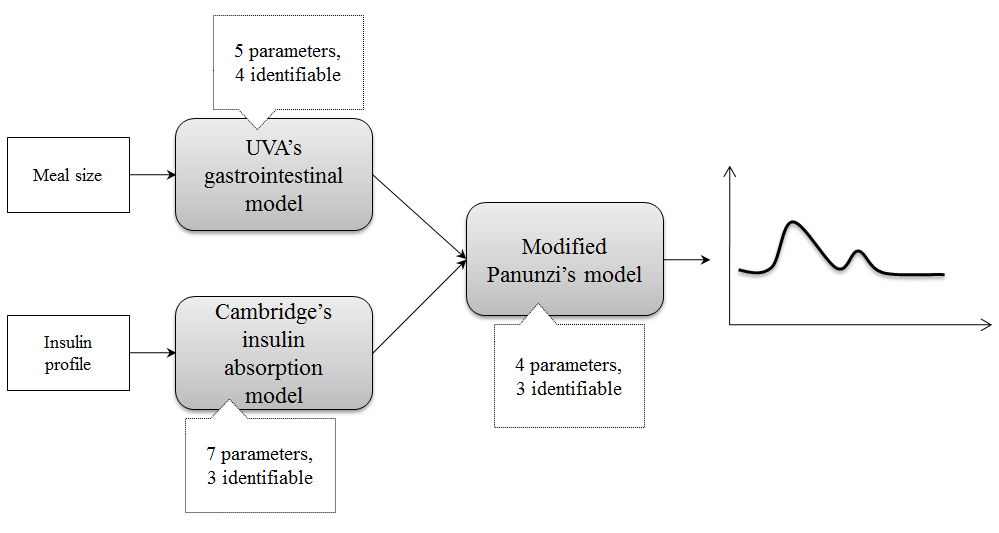
\epsfig{file=Figures/panunziparametersidentifiable.png, width=\textwidth}\caption{Optimal set of parameters for the modified Panunzi's model combined with UVA's gastrointestinal model and Cambridge insulin absorption.}
\label{fig:panunziparametersidentifiable}
\end{figure}

These 10 parameters will be used in the experiment design for the calculation of the index of total identifiability of the model. All identifiable parameters are distributed amongst all the submodels of the modified Panunzi's system. The same approach of multiple day identifications used for the optimal experiment design of Bergman's model is used in here. In the next lines, experiments designed comprising one, two, three and four days of monitoring are displayed.

\begin{itemize}
\item{The results of an experiment designed for \textit{one} day of monitoring consisting on the five following hours to a meal are: $\tau = -17.95$ minutes, Meal $= 100$ g CHO and Bolus $=10$ IU. The same profile as in the Bergman's model experiment design is observed in the modified Panunzi's experiment for the one-day monitoring. The insulin bolus is not as advanced as in Bergman's model design, but the meal and bolus size are again in the maximum value of the constrained optimization. Separation of dynamics of the insulin absorption system is the best option for the one-day monitoring scenario. The response of the new model to the experiment designed is shown in Figure \ref{fig:optdesignpanunzi1day}.

\begin{figure}[hbt]
\centering
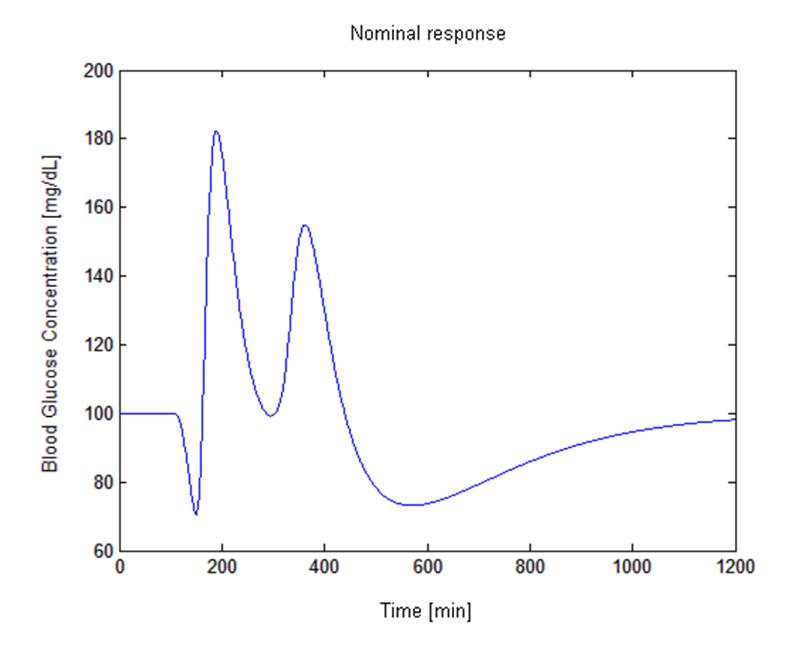
\epsfig{file=Figures/optdesignpanunzi1day.png, width=0.9\textwidth}\caption{Modified Panunzi's model response to the proposed experiment for 1 day. Meal is ingested at time 120 min.}
\label{fig:optdesignpanunzi1day}
\end{figure}

Comparing modified Panunzi's model response in a single day experiment with the Bergman's model response (Figure \ref{fig:bergmanexperiment1day}), the glucose profile is virtually identical. This fact may lead to two conclusions: 1) Using simple endogenous models, the dynamics of the input models direct the behavior of glucose concentration; 2) the optimization of identifiability is not strongly dependent on the endogenous models used. Indeed the model's parameters are different in each model, but the signal from where information is being extracted is the same, and regarding that signal from a theoretical point of view, the optimal glucose profile in terms of containing information, must be very rich in information for any other model too. That is why it is expected of optimal experiment glucose outcomes to be similar for the modified Panunzi's model to the results for the other experiments already designed.}

\item{The conditions of experiment designed \textit{two} day monitoring are:

\begin{itemize}
	\item Day 1. $\tau = 157.80$ minutes, Meal $= 44.25$ g CHO and Bolus $=3.07$ Insulin Units
	\item Day 2. $\tau = -17.92$ minutes, Meal $= 100$ g CHO and Bolus $=9.99$ Insulin Units
\end{itemize}

The second day in this experiment is the same as the single day experiment, in which the bolus is administered in advance to the meal time, thus only the insulin system is being excited in that period. In the first day, a new situation is proposed, similar to the case of Bergman's design in which the bolus was delayed, but in this case, the delay is much bigger. However, delaying the insulin bolus up to two hours and a half can be quite dangerous for the patient because of risks of hyperglycemia, that is why the meal size is much smaller for this large delay case, in order to keep the glucose profile within safety constraints. In Figure \ref{fig:optdesignpanunzi2day} the response of the model to the experiment proposed can be observed.

\begin{figure}[hbt]
\centering
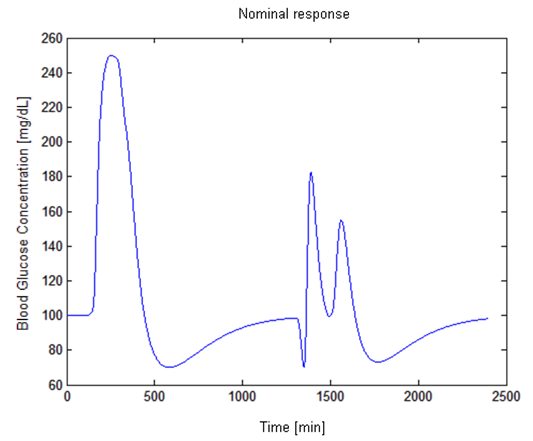
\epsfig{file=Figures/optdesignpanunzi2day.png, width=0.9\textwidth}\caption{Modified Panunzi's model response to the proposed experiment for a 2 days monitoring. Meals are ingested at time 120 and 1020 min.}
\label{fig:optdesignpanunzi2day}
\end{figure}

In the case of the first day  the small amount of carbohydrates given to the patient (44.25 grams) has the objective of rising the blood glucose up to the superior limit of safety of the patient. The insulin bolus is given when the blood glucose gets to the maximum established, and the amount of insulin given is so that it will force the blood glucose down to the lower safety constraint. Again, the experiment design is exciting the glucose signal used for identification from one boundary to the other, in order to maximize the amount of information contained in the glucose signal. Bergman's model was probably not able rise so fast up to the limit of hyperglycemia due to the so called term of glucose efficiency (as explained in Section \ref{sec:CriticalSelectionOfModels}) that makes glucose to drop automatically when it rises above the stability point. As this term is not present in the modified Panunzi's model, glucose dynamics are much faster and permit stronger excitations from the inputs, which is more realistic.}

\item{The conditions of experiment designed \textit{three} day monitoring are:
\begin{itemize}
	\item Day 1. $\tau = -17.83$ minutes, Meal $= 100$ g CHO and Bolus $=10$ Insulin Units
	\item Day 2. $\tau = -18.42$ minutes, Meal $= 100$ g CHO and Bolus $=10$ Insulin Units
	\item Day 3. $\tau = 165.74$ minutes, Meal $= 44.38$ g CHO and Bolus $=3.01$ Insulin Units
\end{itemize}


In this case the advanced bolus administration is given in two out of the three days of the experiment, while the other day a small meal is given, with the insulin bolus delayed 165 minutes, just like in the two days experiment. The fact that the ``bolus given in advance'' scenario is repeated proves that there is more information to be extracted from the excitation of the insulin absorption model than in the rest of the system. This conclusion is repeated for both model's experiment design. The simulated glucose profile of the model is shown in Figure \ref{fig:optdesignpanunzi3day}.

\begin{figure}[hbt]
\centering
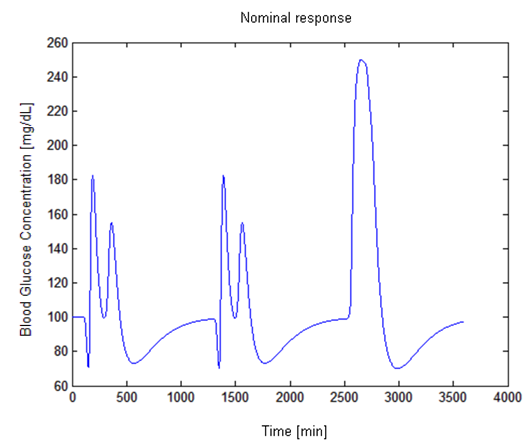
\epsfig{file=Figures/optdesignpanunzi3day.png, width=0.9\textwidth}\caption{Modified Panunzi's model response to the proposed experiment for a 3 days monitoring. Meals are ingested at time 120, 1020 and 1920 min.}
\label{fig:optdesignpanunzi3day}
\end{figure}


This is a very good example of how the different experiments designed for each independent day are not dependent on the order of those days. Sometimes the case of the small meal and delayed bolus happens in the first day, some others at the end, and it can also be in the middle of the 3 days. Also, it is confirmed that increasing the number of experiments causes the richest information postprandial period to repeat in order to maximize the identifiability. No further synergies between different days where observed, and every day is independent in the optimization algorithm.}

\item{The conditions of experiment designed for the final case of \textit{four} day monitoring are:
\begin{itemize}
	\item Day 1. $\tau = 167.06$ minutes, Meal $= 44.25$ g CHO and Bolus $=3$ Insulin Units
	\item Day 2. $\tau = -17.22$ minutes, Meal $= 100$ g CHO and Bolus $=10$ Insulin Units
	\item Day 3. $\tau = -18.41$ minutes, Meal $= 100$ g CHO and Bolus $=10$ Insulin Units
  \item Day 4. $\tau = 86.19$ minutes, Meal $= 47.07$ g CHO and Bolus $=4.13$ Insulin Units
\end{itemize}

The conditions for day four are a little bit different than the previous ones, but it hardly defines a new type of therapy for a day of identification. It is a variation of the profile with a small meal and delayed insulin bolus shown in day one, considering a smaller delay so that the insulin bolus has not only a role of correction of the level of blood glucose, but also tries to counteract the rise of blood glucose that is still coming from the gut. That is observed in Figure \ref{fig:optdesignpanunzi4day}, where the time of administration of the bolus does not wait for the blood glucose to stop rising and get stabilized, and instead, it forces it down before the absorption is over.}
\end{itemize}

\begin{figure}[hbt]
\centering
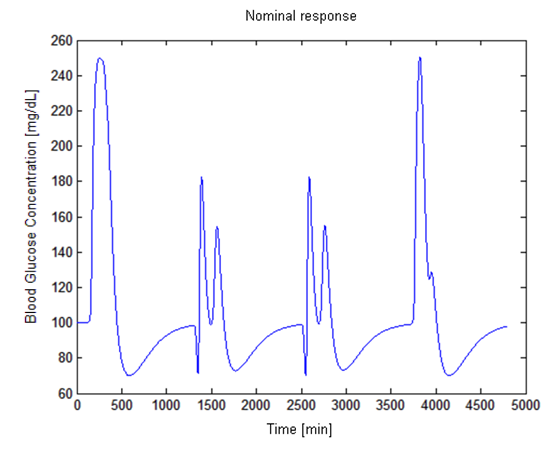
\epsfig{file=Figures/optdesignpanunzi4day.png, width=0.9\textwidth}\caption{Modified Panunzi's model response to the proposed experiment for a 4 days monitoring period. Meals are ingested at time 120, 1020, 1920 and 2820 min.}
\label{fig:optdesignpanunzi4day}
\end{figure}

As a summary, with the optimal set of parameters of the modified Panunzi's model, two different profiles of glucose are determinant for the good identification of the model.
\begin{itemize}
	\item The first therapy has already been seen in Bergman's model experiment design, and it consists of an advance of the bolus of insulin to the meal time, improving the identifiability of the insulin subsystem.
	\item The second therapy consists on a big delay (2-3 hours) in the administration of the bolus, while giving a small amount of carbohydrates (40-50 grams) to avoid severe hyperglycemia. With this therapy, separation of insulin and glucose dynamic from the meal is obtained, while maintaining plasma glucose in a safe range.
\end{itemize}

In Figure \ref{fig:panunzidays} the evolution with the number of days of the parameters identifiability is shown for the optimal set of parameters.

\begin{figure}[hbtp]
\centering
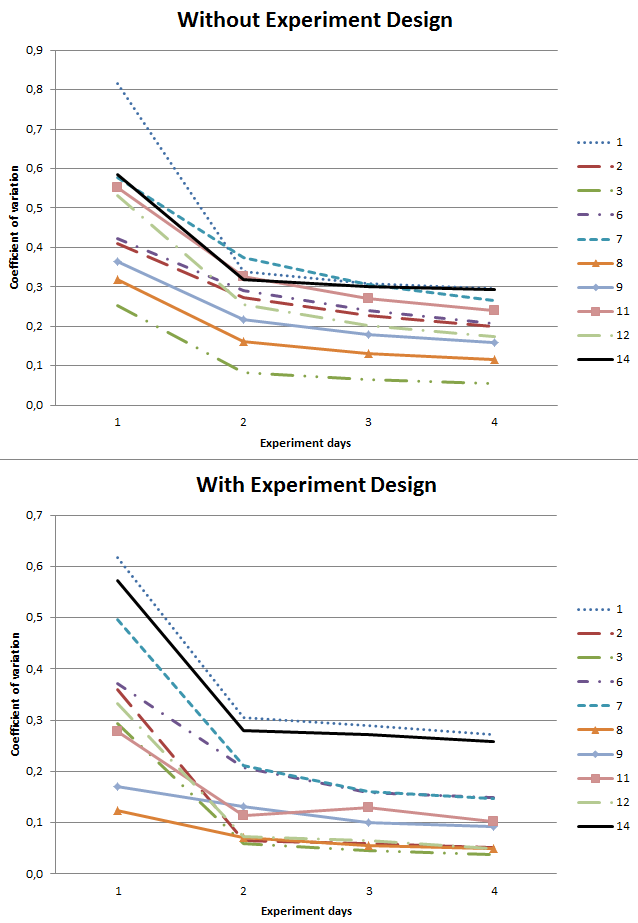
\epsfig{file=Figures/panunzidays.png, width=0.8\textwidth}\caption{Modified Panunzi's optimal set of parameters and their coefficients of variation as they get smaller with the number of monitoring days. Top graph shows the evolution of the parameters' identifiability with experiment length. Bottom panel displays the identifiability of the same parameters applying the designed experiments.}
\label{fig:panunzidays}
\end{figure}

The graphs are very similar to those seen in the analysis of Bergman's model. The influence of the number of days, especially between days one and two, is very important both in the case of experiment and no experiment design. It is worth noting the difference on scale between the top and bottom panel. While without experiment design the parameter's CVs start in some cases as high as 0.8, applying optimization of identifiability this starting variability is reduced to approximately 0.6. Again, a minimum of two days is required for optimal identifiability of the whole system, because of the great drop of CVs of all the parameters in the system, but also because of the inclusion of both therapies proposed which guarantee the separation of dynamics of both input systems. For the same reasons exposed in Bergman's model analysis, a three days experiment is preferred, and it concurs with the findings of the experiment design using modified Panunzi's model.

The influence of the experiment design in the identifiability of the model can clearly be seen in Figure \ref{fig:panunzi1optdesign3days}, where it is shown that experiment design improves identifiability dramatically. In this case, identifiability of almost all the parameters rises, getting their coefficients of variation divided by two or three. Special cases are the parameters 1 and 14, whose identifiability rises to a smaller extent. This resistance to change in the identifiability might be explained by the strong correlation between these two parameters since both of them are very related to the plasma insulin dynamics and its influence in blood glucose (parameter 1, $K_{xgl}$, is the insulin sensitivity and parameter 14, $k_{e}$, is the plasma insulin elimination). On the contrary, $V_g$ identification improves dramatically with experiment design.

\begin{figure}[hbt]
\centering
\epsfig{file=Figures/panunzi1optdesign3days.png, width=\textwidth}\caption{Identifiability of the optimal set of parameters of modified Panunzi's model before and after the experiment design for the case of a three meals monitoring.}
\label{fig:panunzi1optdesign3days}
\end{figure}

\section{Discussion and clinical protocol}
\label{sec:DiscussionAndProtocol}

Identifiability has been drastically improved in both models, but in theory, the experimental design should not end here. The optimal design requires of interaction with the experimental setup in order to keep improving the conditions of the identification. For example, the assumption of nominal values in the parameters for the analysis and experiment design may be questionable, and every identification performed on real data must be subject to an identifiability analysis. With the collection of new experimental data, we may be able to design further experiments based on a new nominal value on the parameter space.

Up to this point, only two models were tested following the exposed methodology, but the experiment design is open for more models to be challenged in their identifiability. When looking at the identifiability analysis, it was accepted that a parameter was identifiable if its CV was below 0.3. After the optimal experiment design, the optimal set of parameters has had the CVs of all its parameters reduced in many cases far below the 0.3 threshold. Naturally, the question arises: ``what if more parameters were included in the \textit{optimal} set?''. `It is very much possible that those parameters CV drop below the identifiability threshold after the optimization of identifiability. However, it is impossible to know this \textit{a priori}, and a iterative approach must be used to check this hypothesis. Unfortunately, optimal experiment design is a very heavy computation task, and embedding it in an iterative paradigm seems unreasonable, and thus this hypothesis is discarded.

The results of the experiment design do not have to be taken literally in practice. The assumptions made when using each model with its nominal parameters have great importance on the results of the experiment design. From a practical point of view, experimenting with several different models allows us to draw some general qualitative conclusions. That is why the design has been repeated several times in this thesis. Qualitative and common characteristics of the experiments designed are extracted in the next lines, trying to get the most important features needed in a monitoring for the good posterior identification of a patient, regardless of the model used.

The experiment design aims to separate the dynamics of the sub-models for a better identification. There are two different single day experiments present: in one case insulin dose is given without meal perturbation, limited by the hypoglycemia constraint, in order to obtain information of the subcutaneous insulin model. The other situation is exactly the opposite: a meal is given while the insulin dose is delayed limited by the hyperglycemia constraint. During this time, the intestinal absorption model is the only one acting on the output signal. Optimal experiment design forces the model to move in all the range of operation set in order to preserve patient's safety, thus extracting more information out of the data. Maximum excitation of the model is required, while separating the perturbations to the output signal for maximum identifiability.

The application of the designed experiment in ambulatory conditions is not straightforward. In the optimal experiment design the (virtual) patient is supposed to be stabilized into euglycemic range. In real experiments, even during the fasting state, patients may not be under steady state conditions, presenting glucose concentration measurements in any glycaemic range. Under these circumstances, application of the optimal experiment design to the clinical setting requires some cautions. Indeed, if the patient is hyperglycemic at the beginning of the experiment, delaying more than two hours the insulin dose can be dangerous for the patient's health, with extremely high glucose values. On the other hand, if the patient is hypoglycemic (or prone to hypoglycemia) in the preprandial period, administrating an insulin dose without carbohydrates ingestion can lead to severe hypoglycemia. 

Therefore, an adaptation of the optimal experiment design to the initial metabolic state of the patient is proposed \cite{DTMlaguna2010}. For every major meal of the day, if the patient starts the monitoring with a blood glucose level over 150 mg/dL or in the 100-150 mg/dL range with an increasing trend (hyperglycemic risk), the insulin bolus is given followed 30 minutes later by a 100 grams meal. If the glucose level is below 100 mg/dL or in the 100-150 mg/dL range with a decreasing trend (hypoglycemic risk), a 40 or 60 (patient's choice) grams meal is given and the insulin dose administration is delayed 120 minutes. In both situations the dose to be administered is the one recommended to the patient, depending on the size of the meal and his/her usual insulin-to-carbohydrate ratio. The patient can choose among three menus with the same relative nutritional composition. With this protocol the separation of dynamics is achieved, while minimizing risks for the patients. This protocol is summarized in table \ref{tab:protocol}.

\begin{table}[hbt]
	\centering
	\begin{tabular}{| p{0.4\textwidth} | p{0.5\textwidth} |}
	\hline 
	\textbf{Pre-prandial glycemia} & \textbf{Action}\\
	\hline 
	Greater than $150 mg/dL$ or between $100-150$ and rising & Infusion of an insulin bolus 30 minutes before of 100 grams meal \\
	\hline 
	Lower than $100 mg/dL$ or between $100-150$ and decreasing & 40 grams meal and bolus infusion 2 hours later \\
	\hline 
	\end{tabular}
\caption{Clinical protocol for application on ambulatory experiments.}
\label{tab:protocol}
\end{table}

The protocol was approved by the Ethical Committee of the Clinic University Hospital of Valencia and home-made monitoring was performed for validation of the identification procedure. Patients were monitored during two weeks, with a wash-up week in between, and instructed to follow the protocol defined by the experiment design. Twelve subjects with T1DM under long-term intensive insulin treatment with CSII (nine women; 41.8 - 7.3 years old; diabetes' duration, 20.2 - 10.3 years; body mass index, 25.1 - 2.8 $kg/m^2$; glycosylated hemoglobin [A1C], 8.0 - 0.6\%; basal insulin dose, 0.8 - 0.3 U/h; I:CHO ratio, 1.3 - 0.5 U/10 g of CHO [mean - SD]) were studied in the hospital (inpatient study) following a period of ambulatory CGM. In the ambulatory period the subjects underwent at least two outpatient 6-day periods of CGM monitoring for the identification (the first 3 days) and validation (the last 3 days) of an individualized model to be used in the prediction of the 5-h postprandial period. In order to account for intra-patient variability, a prediction model with interval parameters was calculated from the previous identified model considering 20\% uncertainty in insulin sensitivity and 10\% in CHO estimation. The interval model was validated during the last 3 days of CGM, where the patients had a standardized meal daily (40-g, 60-g, or 100-g CHO content, depending on the pre-prandial glucose readings). Unfortunately, validation had to be performed over CGM readings, leading to non-conclusive results. Glucose gold reference data are required for the successful validation of an identification study on diabetic patients, since noisy measurements in the validation days can affect the results of the validation, and therefore the overall performance of the identification experiment.

The data acquired using this protocol was later used to test new computer generated insulin treatments for diabetic patients \cite{paoloibolus2012}. Pilot identifications were performed on the domiciliary data, and the identified models were used for the computation of adjusted-to-patient insulin therapies in a full randomized double-blind study. Although the identification performance was not excellent, they yielded reasonable insulin therapies to be used in clinic that were approved by the medical committee. The main limitation of the identifications performed was that no uncertainty was considered in the identification. Uncertainty was artificially added for the validation, and it was considered to be the same for every patient, which lead to incomplete characterization of the patient. In further experiments, uncertainty must be included in the identification methods.

On the clinical part of the experiments performed, subjects were admitted to the Endocrine Clinical Research Center of the Clinic University Hospital of Valencia, Valencia, Spain, at 09:00 h. They were put in the sitting position, and two venous lines were prepared: one for arterialized venous blood sampling and the other for insulin or glucose infusion, if required. Indeed, to ensure comparable metabolic conditions between studies, where appropriate, subjects received an intravenous infusion of regular human insulin following a feedback procedure to maintain PG close to 90 mg/dL until the beginning of the studies at 13:00 h (time 0 of the study). Then, the test mixed-meal was consumed in 15-20 min. At the same time, insulin was administered following the randomization schedule, and PG was monitored for 5 h, until the end of study at 18:00h (time 300 min). In order to avoid hypoglycemia during time 0-300 min, a controlled glucose infusion was started if blood glucose fell below 75 mg/dL, and the pre-meal glycaemic levels were maintained (euglycemic clamp). 

Similar results were observed in the in-hospital part of the experiment for the regular insulin treatment, which is adjusted by medical experts, and the computer generated insulin therapy. This findings lead to the conclusion that CGM-based algorithm for the calculation of prandial insulin is feasible, although it does not reduce unpredictability of individual glycaemic responses.




		
\chapter{CGM Statistical Modeling and Validation}
\label{sec:CGMStatisticalModelingAndValidation}

Identifiability is highly dependent on the quality of the measurements obtained. In this chapter the focus will move from the improvement of experiments towards the analysis and improvement of data acquisition devices. Sensor induced errors are one of the main problems in diabetes experimentation nowadays. Continuous glucose monitoring (CGM) devices estimate plasma glucose from interstitial glucose measurements every 1-5 minutes. They are potentially much more informative than the traditional and sparse method based on capillary self-monitoring of blood glucose. However, CGM devices are only approved as adjunctive to capillary self-monitoring due to their low accuracy.

Despite its relevance to the interpretation of glycaemic time-series and to the implementation of a future artificial pancreas, few studies have investigated the error characteristics of current CGM devices, especially in the postprandial state. Breton \textit{et al.} \cite{breton2008analysis} developed an error model for CGM based on a posteriori recalibrated data from the FreeStyle Navigator\texttrademark  (Abbott Diabetes Care, Alameda, USA). However, in contrast to real-time calibration algorithms, a posteriori recalibration implies the use of all reference BG points to minimize the sensor readings-reference glucose mismatch. In addition, Facchinetti \textit{et al.} \cite{facchinetti2010modeling} demonstrated using simulation studies how small errors in data recalibration can affect the derived statistical properties for the error. Recently, Facchinetti \textit{et al.} published a study \cite{facchinetti2013modeling} on the error of the SEVEN\textsuperscript{\textregistered} PLUS sensor (also under review in this thesis) where the diabetic subjects wore four sensors during a 9 hour study, to a total of 36 monitoring sessions. The sensors were tested against a HemoCue Glucose 201 Analyzer, using standard calibration procedures. The sensors showed clear correlations between them, and AR models were used for adjustment of the error, providing an accurate CGM error model and the factor that compose them. No simulation model of the sensor was provided, and no correlation with the blood glucose signal was provided. Therefore, error characterization of real-time CGM devices in the postprandial state is still an open issue and an area for additional investigation.

In this chapter an analysis and modeling of the postprandial error of two commercial real-time CGM devices is performed, namely the Dexcom\textsuperscript{\textregistered} SEVEN\textsuperscript{\textregistered} PLUS and the Medtronic\textsuperscript{\textregistered} Paradigm\textsuperscript{\textregistered} Veo\texttrademark{}, that were simultaneously worn by subjects with type 1 diabetes following a set of four standardized mixed meals. Statistical properties of the signal error were analyzed and a new simulation model was generated aiming for its integration into in silico studies.

\section{Data and methodology}
\label{sec:MethodologyAndData}

Twelve subjects with type 1 diabetes treated with continuous subcutaneous insulin infusion (CSII) (male/female 3/9, age $41.8�7.3$ years, diabetes duration $20�10$ years, HbA1c $8.0�0.6\%$) were studied in the postprandial state under controlled conditions, on four different occasions. Patients were monitored twice when eating a standardized meal with 40 g CHO content and twice, in addition, when they received a 100 g CHO meal. On each occasion, CGM was performed simultaneously with a SEVEN\textsuperscript{\textregistered} PLUS (Dexcom, San Diego, USA) device and a Paradigm\textsuperscript{\textregistered} Veo\texttrademark{} (Medtronic, Northridge, USA) device. 

Both devices were inserted the day before the experiment, in order to allow the devices to stabilize before the experiments. During the first day the monitors were calibrated according to the manufacturer instructions using the same capillary measurements. The day of the experiment, the devices were calibrated using the same capillary measurement obtained in fasting state.

The patients arrived at 9:00 AM to the clinic. Pre-prandial plasma glucose was standardized around 100 mg/dL by means of a feedback insulin infusion. At 13:00 h, patients ate the standardized meal and received the corresponding insulin bolus using a subcutaneous insulin infusion system. Plasma glucose levels were measured for 5 hours after the meal, every 5 minutes the first two hours after the meal and every 10 minutes afterwards, thus obtaining more frequent measurements during the meal rise phase. Plasma blood glucose levels were measured on arterialized venous blood using a reference method (YSI 2300 STAT Plus Glucose analyzer, YSI Yellow Springs, Ohio, USA), and synchronously compared with CGM's subcutaneous measurements (5 min frequency). Only forty-seven datasets were available for analysis when the SEVEN\textsuperscript{\textregistered}  PLUS device was used, because one dataset was discarded due to a flat sensor measurement at 40 mg/dL during the whole duration of the experiment. In the case of the Paradigm\textsuperscript{\textregistered} Veo\texttrademark{} device, only 42 datasets were available because the first 6 experiments were not monitored with this device. 

YSI data is assumed to be very accurate, especially if compared with any CGM device. Nowotny \textit{et al.} \cite{nowotny2012precision} evaluated the accuracy of the YSI 2300 Glucose Analyzer among other devices, showing errors of 2.2\% . This is higher than previous reference methods, and also better than the rest of the analyzers evaluated.

In order to obtain a time series of the same sample size, YSI data were linearly interpolated in the late postprandial period in order to obtain a 5 minutes periodic consistent dataset, and be able to compare it with the CGM data. Although interpolation of reference data can introduce undesired dynamics when modeling, in this case interpolation only occurs in the late postprandial period, where dynamics of both the glucose and the monitor were slower. In addition, linear interpolation were used in literature before, in the context of glucose modeling of sensor signals \cite{breton2008analysis,facchinetti2007reconstruction} where reference measurements were sparse (15 minutes). 

The signal analyzed was the CGM error calculated as:

\begin{equation}
	E(k)=CGM(k)-YSI(k)
\label{eq:cgmerror}
\end{equation}

where $E(k)$ is the error at time $k$, $CGM(k)$ is the CGM signal and $YSI(k)$ the reference blood glucose, both at the same time $k$. Some issues were taken into account in the analysis. First, the existence of a physiological delay between subcutaneous and plasma glucose, which could be patient-specific \cite{kamath2009analysis}. Second, filters included in the CGM devices may introduce additional delays (signal-processing delays). Both types of delays represent a confounder factor of CGM accuracy and should be compensated prior to further study of the error.  Third, stationarity of the error time-series should be investigated since non-stationarity may yield misleading probability distributions. Indeed, when fitting probability distribution and time-correlation of a signal, stationarity of the process is assumed. In the event of having a time varying stochastic process, non-linear transformations must be applied to the signal so that it becomes as time unvarying as possible \cite{box1994time}. The choice of the non-linear transformation to be used usually depends on the problem and the data available. 

\begin{figure}[hbtp]
\centering
\epsfig{file=Figures/CGMmodelflow.png, width=\textwidth}\caption{Summary of stepwise statistical analysis process.}
\label{fig:CGMmodelflow}
\end{figure}

The analysis described in Figure \ref{fig:CGMmodelflow} was followed for both CGM devices:

\begin{enumerate}
	\item The delay of the CGM signal with respect to reference glucose was computed as the lag with maximum CGM versus YSI cross-correlation for each patient. A probability distribution function was fitted to the delay's histogram using a classical maximum likelihood (ML) estimator from Matlab Statistics Toolbox. Error time-series were then shifted by the corresponding delay for compensation prior to next analysis thus ``synchronizing'' CGM and reference glucose signals.
	\item Stationarity of the shifted error time-series was analyzed. A signal was considered to be stationary if time invariance of the statistical moments held. Mean and standard deviation of the error signal were calculated across the population of sensors in every instant of the postprandial period in order to obtain a time dependent signal. Time dependence of the mean and the standard deviation was analyzed. Besides graphical inspection, datasets were fitted to autoregressive (AR) models and the presence of a unit root was investigated (random walk process in the case of first order models). A stationary process should have no unit roots.
	\item Finally, the sample probability distribution for the error was analyzed and an AR model fitted to reproduce time correlation and for simulation purposes. A set of candidate probability distribution functions was defined and ML estimators in Matlab Statistics Toolbox were used for data fitting for every distribution. A simple quadratic error index was used to measure the fit for comparison purposes.
\end{enumerate}

	When performing a linear regression or just a simple correlation between variables, correlations were tested to be statistically significant using a t-statistic testing the null hypothesis of non-correlation

\section{CGM Modelling}
\label{sec:CGMModelling}

Both CGM devices were first compared to the reference measurements in order to get a general error magnitude of each error. For this comparison, the MARD (Mean Absolute Relative Deviation) was computed, following the next formula:

\begin{equation}
  MARD:= \frac{\sum_{i=1}^{n} \left| (CGM_i - YSI_i) / YSI_i \right| \cdot 100}{n}
\label{eq:mard}
\end{equation}

where $n$ is the number of samples, $CGM_i$ stands for the sensor glucose reading at time $i$ and $YSI_i$ is the reference glucose at time $i$. The SEVEN\textsuperscript{\textregistered}  PLUS monitor showed a MARD of 17.28\%, and the VEO monitor 20.12\%, for the whole dataset. 

\begin{figure}[hbtp]
\centering
\epsfig{file=Figures/errorgrids.png, width=\textwidth}\caption{Clarke error grid (EGA) and rate error grid from continuous glucose-EGA plots for both monitors. Top row shows Clarke EGA plots, observed glucose reference measurements \textit{versus} the prediction of the monitors, SEVEN\textsuperscript{\textregistered} PLUS on the left and VEO on the right. On the bottom row, the rate error grid from continuous glucose-EGA is displayed, for the SEVEN\textsuperscript{\textregistered} PLUS on the left and VEO on the right.}
\label{fig:errorgrids}
\end{figure}

Clinical accuracy for both datasets is illustrated in Figure \ref{fig:errorgrids} using two complementary error grid analysis (EGA) methods: the Clarke-EGA \cite{clarke1987evaluating} and the glucose-rate grid proposed by Kovatchev \textit{et al.} \cite{kovatchev2004evaluating}. Regarding the Clarke grid, both monitors show very similar behavior. The SEVEN\textsuperscript{\textregistered} PLUS monitor placed 73.04\% of the data pairs in zone A, and 26.41\% in zone B, while Veo system had 66.23\% of the data pairs in zone A, and 33.25\% in zone B. Both monitors had less of 1\% of the monitoring data within the zones C, D or E. Regarding the glucose rate grid, the SEVEN\textsuperscript{\textregistered} PLUS monitor had 80.96\% of data points in zone A, 14.89\% in zone B, 2.41\% in zone C, 1.42\% in zone D and 0.32\% in zone E. Veo monitor showed 83,37\% of the data points within the zone A, 13.53\% in zone B, 0.67\% in zone C,  2.10\% in zone D, and 0.31\% in zone E.

A representative CGM trace from each device is shown in Figure \ref{fig:CGMsamples}. The YSI signals shown correspond to different patients following the detailed experiments. In the SEVEN\textsuperscript{\textregistered} PLUS monitor sample, a rapidly increasing glucose concentration after the meal is observed, followed by a slow decreasing glucose in the late postprandial period. The VEO monitor sample shows a rapidly increasing glucose response right after the meal and a rebound increase in the late postprandial period. It can be appreciated that both monitors have trends similar to the YSI signal they are estimating.

\begin{figure}[hbtp]
\centering
\epsfig{file=Figures/CGMsamples.png, width=\textwidth}\caption{Representative sample of two different postprandial periods for the two monitors. The left panel shows the SEVEN\textsuperscript{\textregistered} PLUS monitor sample and the right panel shows the VEO monitor sample.}
\label{fig:CGMsamples}
\end{figure}

\subsection{Analysis of delay}
\label{sec:AnalysisOfDelay}

The delay histogram for all the available datasets is shown in Figure \ref{fig:delaymodelfit}. This delay was consistent throughout the entire postprandial period, and no significant difference on the calculated delays was achieved by considering only the first two hours (transient) of the entire postprandial period. Observing the time correlation of the datasets, in the SEVEN\textsuperscript{\textregistered} PLUS monitor, 28 showed no significant delay between the two signals (i.e, delay was less than five minutes due to the CGM resolution), and 19 for the Paradigm\textsuperscript{\textregistered} Veo\texttrademark{} .

\begin{figure}[hbtp]
\centering
\epsfig{file=Figures/delaymodelfit.png, width=\textwidth}\caption{Delay-time histograms for the SEVEN\textsuperscript{\textregistered} PLUS monitor (left) and the Paradigm\textsuperscript{\textregistered} Veo\texttrademark{} (right).}
\label{fig:delaymodelfit}
\end{figure}

The histogram analysis hinted that the delay follows an exponential probability distribution:
\begin{equation}
  f(x)=\frac{1}{\mu} e^{-\frac{x}{\mu}}
\label{eq:exponential}
\end{equation}

where $\mu$ is the exponential parameter. The exponential parameter was adjusted for each monitor. For the SEVEN\textsuperscript{\textregistered} PLUS monitor the parameter was $\tau_{sevenplus}=1.08$ with a 95\% confidence interval $[0.82,1.46]$ and for the Paradigm\textsuperscript{\textregistered} Veo\texttrademark{} $\tau_{veo}=1.69$ with a 95\% confidence interval $[1.28,2.35]$, resulting in the curve fitting shown in red in Figure \ref{fig:delaymodelfit}.

The observed delay for the SEVEN\textsuperscript{\textregistered} PLUS device was consistent with previous works \cite{zisser2009accuracy} for the SEVEN\textsuperscript{\textregistered} system, where an average value of 5 minutes is reported as the lag for maximum cross-correlation. However, no probability distribution for the delay was reported for comparison. Compared with the Dexcom system, the Paradigm\textsuperscript{\textregistered} Veo\texttrademark{} showed a significant (p=0.007) larger average delay (8 minutes). Our results were slightly larger than those reported by Keenan \textit{et al.} \cite{keenan2010accuracy}, but neither these values nor the SEVEN\textsuperscript{\textregistered} Plus values were comparable due to the difference in computation methods. Therefore, measurement of the delay should be standardized in order to enable comparisons between different studies. Additionally, the Paradigm\textsuperscript{\textregistered} Veo\texttrademark{} exhibited a slower decay in the fitted exponential distribution, indicating higher variability of the delay value up to 30 minutes. 

\subsection{Analysis of Stationarity}
\label{sec:AnalysisOfStationarity}

The statistical moments of the data analyzed after delay compensation were not time invariant, as shown in Figure \ref{fig:stationarityexperimental}. For both monitors, the mean and standard deviation of the error were non-stationary. Our goal was to find a transformation of the signal in order to make it as close to stationary as possible. This transformation had to be invertible for simulation purposes. This means that the transformation had to be based on available information in the simulation context, e.g., plasma glucose from a glucoregulatory model, or equivalently, the YSI signal from the experimental data.

\begin{figure}[hbt]
\centering
\epsfig{file=Figures/stationarityexperimental.png, width=\textwidth}\caption{Top panels show the meal error and standard deviation of the error after delay compensation for the SEVEN\textsuperscript{\textregistered} PLUS and the Paradigm\textsuperscript{\textregistered} Veo\texttrademark{} monitors. Bottom panels show the same signals after the standardization process. The left figures show the mean error for both monitors while on the right the standard deviation of the error signals is represented. Notice the different scales on all four plots.}
\label{fig:stationarityexperimental}
\end{figure}

In general, stationarity of the error time-series is assumed when fitting probability distributions to a stochastic signal. However, it can be observed that these assumptions were not correct when interpreting the error of CGM in the postprandial state. Mean and standard deviation after delay compensation were both time-varying, especially for the first two hours after a meal intake. This may be related to the performance of the real-time calibration algorithm after the high rise of glucose following the intake up to its peak value.

Despite the standardization of the initial conditions by means of an insulin feedback phase, both monitors had an initial mean underestimation of glucose of 10 mg/dL. Surprisingly this value was equal to both devices. It is unknown to the author whether it may correspond to a setting of the manufacturers. An initial standard deviation of 20-25 mg/dL was observed yielding significant errors. 

Both monitors were worn simultaneously by the patient and calibrated with the same calibration points obtained in fasting state the same day of the experiment. Calibration points have been recognized as crucial factors influencing the accuracy of CGM readings \cite{buckingham2006,wolpert2008}. In this case, the calibration performed was done 4-5 hours before the experiment in fasting state, and it did not seem to induce differences between both devices.

After meal intake, both devices were unable to follow the high rise of glucose, increasing the initial underestimation up to a peak value (approximately 20 mg/dL for SEVEN\textsuperscript{\textregistered} Plus and 30 mg/dL for the Paradigm\textsuperscript{\textregistered} Veo\texttrademark{}) about 50 minutes later. The particular sensor delay should be additionally considered for a correct interpretation. During this time, the error standard deviation increased steadily, having a similar peak time as the mean error, with a peak value of 35 mg/dL for both monitors. 

After this initial period, the glucose underestimation decreased. The CGM glucose estimation recovered slowly towards the glucose reference value. A faster recovery was observed by the SEVEN\textsuperscript{\textregistered} PLUS. It is noteworthy that approximately zero mean error was observed for the SEVEN\textsuperscript{\textregistered} PLUS monitor after peak time, in contrast to VEO signal, which appears to be showing a bias in the mean error. This bias converged slowly to zero, but the 5 hours postprandial monitoring window we used here was insufficient for capturing the whole stabilization of the mean error in the VEO monitor.

If variability of CGM readings were reduced, our results suggest that CGM would allow for a good representation of postprandial glucose. Regarding the standard deviation, a plateau at 35 mg/dL was reached for the SEVEN\textsuperscript{\textregistered} PLUS, while a slight increasing trend was obtained for the Paradigm\textsuperscript{\textregistered} Veo\texttrademark{}. Thus, the meal event represented a big challenge for both devices producing a significant variability, which is still a major issue in CGM performance. Certainly, sources of this variability should be investigated in future studies to confirm whether it is due to variability of the physiological delay, the intensity signal produced by the sensor or the calibration algorithm itself. 

A positive correlation between the YSI signal and the standard deviation of the error was found. This is an indication of the variability of the sensor to capture the postprandial peak. In addition, a negative correlation of the YSI rate of change and the mean of the error reflects that sensor readings were falling behind the reference glucose in the rising trend (the error becomes more negative in average), in spite of delay compensation. 

The second moment of the error signal closely resembled the YSI blood glucose measurements for both monitoring systems. The correlation coefficient for the SEVEN\textsuperscript{\textregistered} PLUS monitor was $r_{sevenplus}=0.93$ ($range_{95\%} = [0.90, 0.96]$) and for the Paradigm\textsuperscript{\textregistered} Veo\texttrademark{} $r_{veo}=0.82$ ($range_{95\%} = [0.72, 0.89]$), both significant ($p<0.005$). The regression lines for these correlations were:
\begin{align}
	\text{SEVEN PLUS: }STD(k) &=0.3142 \cdot YSI(k)-12.9056 \label{eq:std_corr1} \\
	\text{VEO: }STD(k) &=0.2711 \cdot YSI(k)-3.7679 \label{eq:std_corr2}
\end{align}

where $STD(k)$ is the standard deviation of the error at time $k$. 

As for the mean of the error signal, the correlation with the raw YSI signal did not show a significant correlation coefficient. The correlation with the gradient of the YSI signal was better, with a coefficient of $r_{sevenplus}=-0.79$ ($range_{95\%} = [-0.87, -0.68]$) and $r_{veo}=-0.54$ ($range_{95\%} = [-0.70, -0.33]$), both being statistically significant ($p<0.005$). This correlation was not as evident as the one with the second moment, but it was much better than the correlation found to any other signal derived from the YSI. Regarding to the correlations found we can guess that stationarity achieved with these transformations was better in the SEVEN\textsuperscript{\textregistered} PLUS monitor than in the Paradigm\textsuperscript{\textregistered} Veo\texttrademark{}. The regression line for the correlation of the first moment was:
\begin{align}
	\text{SEVEN PLUS: } & Mean(k)=-2.0046\cdot dYSI(k)/dt-1.0628 \label{eq:mean_corr1} \\ 
	\text{VEO: } & Mean(k)=-1.323\cdot dYSI(k)/dt-10.517 \label{eq:mean_corr2}
\end{align}

where $Mean(k)$ is the average error at time $k$.
Again, as it happened with the delays, these regressions were consistent throughout the entire postprandial period. Considering these regressions as good characterizations of the statistical moments of the signals, the error signal can be transformed as follows, so that it becomes (quasi-)stationary: 

\begin{equation}
	\bar{E}(k)=\frac{E(k)-Mean(k)}{STD(k)}
\label{eq:error_standard}
\end{equation}

In case of perfect estimation of the mean and standard deviation at time $k$, the transformed error signal $\bar{E}(k)$ will have zero mean and unity standard deviation throughout the postprandial period.

Stationarity of the signal was improved after this transformation, as shown by the roots of the AR models fitted before and after the ``standardization''. The error signals were tested to fit AR models, looking for the lowest-order model with random uncorrelated residuals. The transformed statistical moments along time can also be seen in Figure \ref{fig:stationarityexperimental}, where a clear improvement on stationarity of both signals can be appreciated comparing top and bottom panels.

The SEVEN\textsuperscript{\textregistered} PLUS time-series showed a good fitting to a first order AR model before and after the transformation. The model root was $z=0.9892$ before the transformation, and $z=0.9249$ after. The transformation moves the dynamics of the data away from those of a random walk (unit root), thus making it more stationary.
The Paradigm\textsuperscript{\textregistered} Veo\texttrademark{} time-series adjusted well to a first order AR model before the transformation and to a third order model after. The model root before the transformation was $z=0.9977$, reaffirming the non-stationarity of the process. After the transformation, the model root closer to unity was $z=0.9846$, showing some improvement towards stationarity, but not as much as in the SEVEN\textsuperscript{\textregistered} PLUS. Correlations were weaker in the case of the Paradigm\textsuperscript{\textregistered} Veo\texttrademark{} which translated into a worse compensation for non-stationarity.

\subsection{Distribution fitting}
\label{sec:DistributionFitting}

The datasets used for distribution and auto-correlation fitting were already transformed following the delay compensation and the standardization processes explained before. Kurtosis was high for both datasets, so leptokurtic distributions were used for fitting. Asymmetry was very low in the data, but some non-symmetric distributions were also tested. Four different statistical distributions were finally considered:
\begin{align}
	\text{Weibull: }  f(x) & =\frac{k}{\lambda}\left( \frac{x}{\lambda}\right)^{k-1} e^{-\left(x/\lambda \right)^k} \label{eq:distributions1} \\  
	\text{Normal: } f(x) &=\frac{1}{\sqrt{2 \pi \sigma^2}} e^{-(x-\mu)^2 /2 \sigma^2} \label{eq:distributions2} \\ 
	\text{Log-Normal: }  f(x) &=\frac{1}{x \sigma \sqrt{2 \pi \sigma^2}} e^{-(log x - \mu)^2 /2 \sigma^2} \label{eq:distributions3} \\ 
	\text{Logistic: } f(x) &=\frac{1}{1+e^{\frac{x-\mu}{s}}}  \label{eq:distributions4}
\end{align}

Five Paradigm\textsuperscript{\textregistered} Veo\texttrademark{} sensors showed unusual behaviors with very big mean absolute errors (over 50 mg/dL), even though their calibrations were correct. These offsets produced a multimodal histogram (see Figure \ref{fig:distributionfit}). Given that this behavior was only observed in 5 sensors, those monitoring periods were not used to fit a probability distribution, remaining a total of 37 datasets. Given that the SEVEN\textsuperscript{\textregistered} PLUS did not register faulty monitoring periods, the Paradigm\textsuperscript{\textregistered} Veo\texttrademark{} seems to be more prone to abnormal sensor behaviors. This should be confirmed with larger studies.


\begin{figure}[hbtp]
\centering
\epsfig{file=Figures/distributionfit.png, width=\textwidth}\caption{Histograms of the standardized error (top) and scaled cumulative distribution (bottom) plots for the SEVEN\textsuperscript{\textregistered} PLUS monitor (left) and the Paradigm\textsuperscript{\textregistered} Veo\texttrademark{} (right).}
\label{fig:distributionfit}
\end{figure}

The Log-Normal and Weibull distributions are only defined for positive values. To cope with this problem, data were transformed by adding its absolute minimum value (equal to 4.3069 for the SEVEN\textsuperscript{\textregistered} PLUS and 2.4439 for the Paradigm\textsuperscript{\textregistered} Veo\texttrademark{}), thus making all errors positive and not centered in zero.
The estimates are shown in Table \ref{tab:distrasults}. The best estimator was given at the normal distribution for the Paradigm\textsuperscript{\textregistered} Veo\texttrademark{} ($\mu_{VEO}=2.435$ and $s_{veo}=0.5415$) and the logistic distribution for the SEVEN\textsuperscript{\textregistered} PLUS ($\mu_{sevenplus}=4.297$ and $s_{sevenplus}=0.587$). Probability plots for the logistic and normal distribution are shown in Figure \ref{fig:distributionfit}. However, the difference between the fit of the logistic distribution and the normal distribution for the SEVEN\textsuperscript{\textregistered} PLUS was almost negligible ($1.92�10^{-3}$ vs $2.02�10^{-3}$). Normality assumption after all the transformations seems thus sensible.

\begin{table}[hbtp]
	\centering
	\begin{tabular}{ c | c | c | c | c | c | c }
	\hline 
	\multirow{2}{*}{Distribution} & \multicolumn{2}{c}{Parameters} & \multirow{2}{*}{Fit$\times 10^{-3}$} & \multicolumn{2}{c}{Parameters} & \multirow{2}{*}{Fit$\times 10^{-3}$} \\
   & \multicolumn{2}{c}{SEVEN\textsuperscript{\textregistered} PLUS} &  & \multicolumn{2}{c}{Paradigm\textsuperscript{\textregistered} Veo\texttrademark{}} & \\
	\hline 
	\multirow{2}{*}{Normal} & $\mu$ & $\sigma$ & \multirow{2}{*}{2.02} & $\mu$ & $\sigma$ & \multirow{2}{*}{1.39} \\
	& 4.27 & 1.057 & & 2.282 & 0.693 & \\
	\hline 
  \multirow{2}{*}{Weibull} & $a$ & $b$ & \multirow{2}{*}{2.49} & $a$ & $b$ & \multirow{2}{*}{2.56} \\
	& 4.652 & 4.329 & & 2.515 & 3.412 & \\
	\hline 
	\multirow{2}{*}{Logistic} & $\mu$ & $s$ & \multirow{2}{*}{1.92} & $\mu$ & $s$ & \multirow{2}{*}{1.84} \\
	& 4.297 & 0.587 & & 2.289 & 0.387 & \\
	\hline 
	\multirow{2}{*}{Log-normal} & $\mu$ & $\sigma$ & \multirow{2}{*}{42.6} & $\mu$ & $\sigma$ & \multirow{2}{*}{42.61} \\
	& 1.402 & 0.764 & & 0.751 & 0.866 & \\
	\hline 
	\end{tabular}
\caption{Parameters of the distribution fitting results for the SEVEN\textsuperscript{\textregistered} PLUS and the Paradigm\textsuperscript{\textregistered} Veo\texttrademark{} monitors.}
\label{tab:distrasults}
\end{table}

Finally, a first order AR model explains appropriately the error data for the SEVEN\textsuperscript{\textregistered} PLUS, which is consistent with Breton \textit{et al.} \cite{breton2008analysis}. However, a third order AR model was needed for the Paradigm\textsuperscript{\textregistered} Veo\texttrademark{}. This may be due to distinct filtering algorithms for the raw signal since both monitors use linear regression based calibration algorithms. Based on the previous analysis a model for each monitor was derived. This model incorporated time-varying statistical characteristics of the error for their integration into in silico tests for controller validations. These models are detailed in the next chapter, along with the full CGM simulation model of each monitor.

\section{Validation}
\label{sec:Validation}

Following the error signal analysis, simulation models were built for the SEVEN\textsuperscript{\textregistered} PLUS and Paradigm\textsuperscript{\textregistered} Veo\texttrademark{}   consisting on the following steps:

\begin{enumerate}
	\item A time series was generated from the fitted AR model.
	\item Transformations applied to get (quasi-)stationarity were inversely applied reproducing time varying characteristics of error mean and variance.
	\item A realization for the delay following the identified probability distribution was computed and applied.
\end{enumerate}

The SEVEN\textsuperscript{\textregistered} PLUS transformed error time-series followed a first order AR model
\begin{equation}
\bar{E}(k) = \alpha_1 \cdot \bar{E}(k-1) + \beta \cdot w(k), \,\,\,\, \bar{E}(0)=w(0)
\label{eq:AR_sevenplus}
\end{equation}
where $\bar{E}(k)$ is the correlated standardized error (output of the AR system), $w(k)$ is a white noise signal, $\alpha_1=0.9249$  is the AR parameter, and $\beta=0.3756$  is the correction of the variance factor, chosen in order to get the desired characteristics of the normal distribution for the data after filtering.  
The Paradigm\textsuperscript{\textregistered} Veo\texttrademark{} time-series followed a third-order model:
\begin{gather}
\bar{E}(k)=\alpha_1 \cdot \bar{E}(k-1)+\alpha_2 \cdot \bar{E}(k-2) +\alpha_3 \cdot \bar{E}(k-3)+\beta \cdot w(k) \nonumber \\
\bar{E}(0)= w(0), \,\,\,\, \bar{E}(1)=w(1) \label{eq:AR3_veo}
\end{gather}
with : $\alpha_1=0.9471$, $\alpha_2=-0.1936$, $\alpha_3=0.2271$ and $\beta=0.2198$.

The white noise used as input of the AR models follows the normal distribution fitted to the data in the previous chapter. Normality was assumed for both monitors. For the SEVEN\textsuperscript{\textregistered} PLUS the mean was $\mu_{SEVENPLUS}=4.27$ and the standard deviation $\sigma_{SEVENPLUS}=1.057$, considering a shift of 4.3069. For the Paradigm\textsuperscript{\textregistered} Veo\texttrademark{} the parameters were: $\mu_{Veo}=2.282$ $\sigma_{Veo}=0.693$, and a shift of 2.4439.

In order to reproduce the time-variance of the error mean and standard deviation, we had to invert the standardization applied to the CGM error data during the analysis process, i.e.:
\begin{equation}
E(k)=STD(k) \cdot \bar{E}(k)+Mean(k)
\label{eq:standardization_invert}
\end{equation}

$STD(k)$ and $Mean(k)$ were calculated as: 
\begin{align} 
	\text{SEVEN PLUS: } STD(k) &=0.3142 \cdot \widetilde{PG}(k)-12.9056               \label{eq:standardization1} \\
	\text{VEO: } STD(k) & =0.2711 \cdot \widetilde{PG}(k)-3.7679                      \label{eq:standardization2} \\
	\text{SEVEN PLUS: } Mean(k) &=-2.0046 \cdot \frac{d\widetilde{PG}(k)}{dt}-1.0628  \label{eq:standardization3} \\
	\text{VEO: } Mean(k) &=-1.323 \cdot \frac{d\widetilde{PG}(k)}{dt}-10.517          \label{eq:standardization4}
\end{align}

where $\widetilde{PG} (k)$ is the plasma glucose given by the virtual patient simulator, or in case of using real patient data, the plasma glucose measurements. The CGM readings were then calculated by adding the error to the simulator glucose output, and shifting $d$ steps, where $d$ is a realization of an exponential distribution $Exp(\mu)$:
\begin{gather}
CGM(k)= \widetilde{PG}(k-d)+E(k-d), \,\, d=Exp(\mu) \nonumber \\
\mu_{sevenplus}=1.08, \,\, \mu_{veo}=1.69 \label{eq:exp_realization}
\end{gather}

An illustration of several simulation runs for both models is shown in Figure \ref{fig:simulatedCGMsamples}. Average MARD for the simulated SEVEN\textsuperscript{\textregistered} PLUS was 18.72\%, and for the simulated Paradigm\textsuperscript{\textregistered} Veo\texttrademark{} was 18.38\%. 

\begin{figure}[hbtp]
\centering
\epsfig{file=Figures/simulatedCGMsamples.png, width=\textwidth}\caption{Three simulation of each monitor with the proposed models for the postprandial period of a virtual diabetic patient. Top panel shows the SEVEN\textsuperscript{\textregistered} PLUS response while bottom panel corresponds to the Paradigm\textsuperscript{\textregistered} Veo\texttrademark{} simulations.}
\label{fig:simulatedCGMsamples}
\end{figure}

For validation purposes a virtual dataset a hundred times larger than the original dataset was created (the model was run a hundred times for each YSI trace), to better simulate the fitted distributions in their entire domain. The YSI samples used for the calculation non-stationarity of the error were extracted from the same dataset used for the model fitting. For this validation, the Paradigm\textsuperscript{\textregistered} Veo\texttrademark{} data used for comparison only comprehends predictions from the 37 sensors than showed no unusual behavior. In Figure \ref{fig:delayvalidation} validation of the signal delay is shown, comparing the probability distribution of the real dataset versus the simulated data. Figure \ref{fig:simulatedstationarity} shows the comparison of the statistical properties of the data and the simulation, as well as illustrates the time variation of the simulated data.

\begin{figure}[hbtp]
\centering
\epsfig{file=Figures/delayvalidation.png, width=\textwidth}\caption{Real and simulated delay distribution for both monitors. The left panel shows the delay of the SEVEN\textsuperscript{\textregistered} PLUS monitor, against the simulation distribution using the proposed model. In the right panel the distributions for the Paradigm\textsuperscript{\textregistered} Veo\texttrademark{} is shown.}
\label{fig:delayvalidation}
\end{figure}

Computer simulations of the adjusted model for both monitors show very similar delay distribution as the original data, as shown in Figure 8. The histograms of both simulated models are much more uniform than the original data, following closely the original exponential distribution that generated them.

\begin{figure}[hbt]
\centering
\epsfig{file=Figures/simulatedstationarity.png, width=\textwidth}\caption{Top row shows time variation of the mean error for both monitors and for the simulated error. In the bottom row the standard deviation of the error and the simulation is plotted against time. Left column shows the SEVEN\textsuperscript{\textregistered} PLUS data and model, and the right column illustrates the statistical behavior of the Paradigm\textsuperscript{\textregistered} Veo\texttrademark{} and its representing model.}
\label{fig:simulatedstationarity}
\end{figure}

Validation of the statistical moments and non-stationarity of the error can be extracted from Figure \ref{fig:simulatedstationarity}. Time variant mean and standard deviation were obtained for the simulated data, with similar dynamics than the original data. Mean signal was almost identical for the SEVEN\textsuperscript{\textregistered} PLUS device, but it showed an offset for the late postprandial period in the Paradigm\textsuperscript{\textregistered} Veo\texttrademark{} simulation (approx. 15 mg/dL). This was expected since the correlations for the Medtronic monitor were much lower than those of the Dexcom device. Standard deviation time variation was also very similar to that of the original error, presenting small offsets at the end of the postprandial period (approx. 5 mg/dL for the SEVEN\textsuperscript{\textregistered} PLUS and 7 mg/dL for the Paradigm\textsuperscript{\textregistered} Veo\texttrademark{}). These offsets did not contribute negatively on the clinical accuracy of the simulated error, since the overall MARD was similar for the simulated dataset and the real data, especially for the SEVEN\textsuperscript{\textregistered} PLUS. Indeed, simulated MARD for the Dexcom monitor was 18.72\%, compared to the 17.28\% of the real monitor. For the Paradigm\textsuperscript{\textregistered} Veo\texttrademark{} the simulated MARD was 18.38\%, being somewhat higher than the observed error from only 37 sensors, which was 14.98\%.

In conclusion, both models were successfully validated reproducing the same statistical properties than the original data. Importantly, although the models have been tested only against postprandial data, additional inconveniences are not expected when analyzing data in the fasting state since postprandial control is considered by far the major challenge in developing the artificial pancreas. Meal intake was a big challenge for both devices, which were unable to follow the high rise of glucose. The high observed variability in both cases threatened postprandial performance. Compared to the SEVEN\textsuperscript{\textregistered} PLUS device, the Paradigm\textsuperscript{\textregistered} Veo\texttrademark{} device seemed to exhibit longer delays and higher probability of abnormal sensor behaviors in postprandial conditions. Certainly, further improvements in calibration algorithms are needed to reduce variability in CGM. 

		
\chapter*{Conclusions}
\label{sec:Conclusions_CGM}
\addcontentsline{toc}{chapter}{Conclusions}

This part of the thesis consisted on parallel work to that of the identification problem in the diabetes context. Foundations for both virtual and experimental identification have been established, and the main contribution of this thesis is now at hand.

Many of the proposed models for diabetic patients suffer from low identifiability. A modification of a literature model was proposed in Chapter \ref{sec:CriticalSelectionOfModels}, but the goal of this model was not to increase current identifiability of the diabetes models but to fit better the physiological properties of the endogenous glucose system of a diabetic patient. Identifiability can be improved in models which have identifiability issues by tuning the conditions of the experiment for better data acquisition properties.

In Chapter \ref{sec:OptimalDesign} a classic optimal experiment design approach was followed for identifiability enhancement. To cope with the inherent problem of model dependance on the experiment results, the procedure was repeated on two different models: the Bergman minimal model and the modified Panunzi's model. The models chosen were amongst the simplest of all the models in literature in order to help in the computation process, which is extremely heavy for the optimal experiment methodology. From the outputs of the experiment design for both models qualitative results were extracted and merged into diabetes experiments guidelines for identifiability optimization.

Three days of monitoring were considered optimal for the current state of CGM. Monitoring sensors are often replaced every week. Considering three days of monitoring for identification, and three or four days for validation, the full lifespan of a sensor is used and more coherent results are expected. Two different profiles were used for the identification days: advance of the meal with respect to the insulin delivery, and delay of the meal. The meal was smaller when advanced and larger when delayed, for patient's safety. The insulin delivery before meal profile was found to enrich the data more than the other profile, being this case repeated twice in the three days experiment.

In the ambulatory environment, the experiments were slightly modified for easier application. The preprandial glucose level and trend were taken into consideration when deciding which of the profiles to apply. Two scenarios were considered:
	
	\begin{itemize}
		\item If preprandial glucose was greater than $150 mg/dL$ or between $100-150$ and rising, the insulin bolus was delivered in advance, followed by a 100 CHO grams meal.
		\item If preprandial glucose was lesser than $100 mg/dL$ or between $100-150$ and decreasing, the insulin bolus was delayed 2 hours to a meal of 40 CHO grams.
	\end{itemize}

This protocol was used for gathering CGM data from 12 diabetic patients in real-life conditions in an experiment in the Clinic University Hospital of Valencia \cite{paoloibolus2012}. Data obtained from those 12 patients in an in-clinic experiment is used later on in this thesis for identification purposes. The same data was used for the development of a simulation model for CGM devices.

The results obtained from the experiment design were tested on two minimal models for sake of simplicity in the design process, and in order to yield results non-dependent on the model. There is no limitation to apply the experiments designed in here to more complex models, such as those used in the patient simulations suites introduced in Chapter\ref{sec:ModelsForDiabetes}. In the following chapters, identification experiments are performed using pre-made interval models based on the Cambridge model. Extensive studies of the properties of this interval version of the Cambridge model can be found in literature, easing the process of simulation. Also, the Cambridge model has been already used in successful closed-loop studies even under domiciliary conditions, which included patient individualization, proving its value for this task.

Two CGM devices were analyzed and modeled in Chapter \ref{sec:CGMStatisticalModelingAndValidation}. The model proposed is stochastic in nature, and can be used for simulation purposes and for testing controllers. Three different characteristics were used for the construction of the model:

\begin{itemize}
	\item Delay of the CGM signal to blood glucose.
	\item Stationarity of the error of the CGM.
	\item Autocorrelation and probability distribution of the error.
\end{itemize}

Delay along the population was found to follow an exponential distribution. Contrary to the general opinion, the error signal of the CGM was found to be non-stationary, and as such much more difficult to model. Very simple correlations were found between the error signal and the blood glucose profile and its derivative. Quasi-stationarity was achieved when using those correlations to transform the error signal. Finally, simple AR models and probability distributions were used for characterization of the stationary signal.

Identification trials on the diabetes context are historically found challenging. Virtual data identification, for example using virtual patient's data from any of the simulators described, is of great importance as an introduction to the real experiments. The CGM model developed in this part of the thesis helps in the completion of virtual identifications for the diabetes context. Compared to other models in literature, the proposed model tackles with the non-stationarity issue as compared to existing models. As for the delay and distribution characterization, the findings of this thesis are in accordance with the results of other publications.





		
		
		\part{Interval identification}
		\label{sec:PartIntervalIdentification}
		
		
\chapter{A New Paradigm for Model Individualization in T1DM}
\label{sec:InSilicoIdentification}

All the mathematical models for T1DM reviewed in this thesis suffer from problems that lead to not mimicking the real patient's physiology. Virtual patient's identification is defined as an identification procedure analog to the experimental data fitting, where the virtual data are generated with the same model used for identification. Uncertainty can be then artificially added to the virtual patient's data to challenge the identification method. The aim of this experiment is to test the methodology of identification in the diabetes context.

Interval models were used for consideration of uncertainty within the diabetic patient, and for the identification fitting. Virtual patients were simulated with inherent variations in their physiologic parameters in order to simulate intra-patient variability. Interval bounding of all the possible outputs of the patients has to be performed for the complete characterization of the patient's data, but overestimation of the uncertainty has to be considered and penalized when using interval models for identification.  From this point of view, we devised another point of view to interval identification. In this thesis, dual objective minimization is used to accomplish interval identification of diabetic patients. the two objectives to be optimized are: 1) the interval data bounding, 2) the glucose interval width. Both objectives are competing in the sense that maximizing the interval output of the model surely will bound more data samples, but the prediction capabilities of the model are worsened.

Multiobjective optimization was then applied to both simulated gold reference data and simulated CGM data of the same patient's, and the results compared.

\section{Optimization Set-up}
\label{sec:MultiobjectiveOptimizationSetUp}

Classic parametric identification results in a single point in the parameter space, being insufficient for the case of a time-varying model based on poor prediction capabilities. Bounding all glucose measurements by means of an interval model, with time-varying parameters considered as intervals, may help identifying both the patient and the intra-patient variability, increasing the robustness of the derived therapies or control algorithms. However, in the case of home monitoring where large measurement errors may appear (especially due to CGM) some relaxation may be needed to avoid large intervals for parameters that loosely fit the physiological variability. 

Identification of interval models has been traditionally addressed under the framework of bounded-error identification (see Chapter \ref{sec:ErrorBoundedEstimation} and references therein). However, when large intra-patient variability is present no parameter values consistent with the error will generally be found. Robust predictions for therapeutic decisions can be achieved if the interval model is able to bound the patient's response, i.e., the experimental measurements should be included in the output envelope predicted by the model at each time instant $t_i$

\begin{equation}
y^{\ast}(t_i) \in y(t_i ;\mathbb{P}), \;\;\; \forall i \in I
\label{eq:measurementscontained}
\end{equation}
	
where $y(t_i ;\mathbb{P})=[\underline{y(t_i ;\mathbb{P}}),\overline{y(t_i ;\mathbb{P})}]$ stands for the interval prediction at time instant $t_i$ for the to-be-identified parameter set $\mathbb{P}$ and $I=\left\{1,...,n\right\}$ is the index set of the available measurements. In practice, a relaxation of the above problem may be needed, allowing for small errors with respect to the inclusion envelope due to noise in the measurements and compensation for non-modeled dynamics. 

Interval parameter values $\mathbb{P}$ must be found so that the model output envelope bounds the measurements. Denoting as $G^{\ast}(t_i)$ the glucose measurement at time instant $i$, equation \eqref{eq:measurementscontained} can be rephrased as:

\begin{equation}
G^{\ast}(t_i) \in [\underline{G(t_i;\mathbb{P})},\overline{G(t_i;\mathbb{P})}], \;\;\; \forall i \in I
\label{eq:measurementscontained2}
\end{equation}

where $\underline{G(t_i;\mathbb{P})}$ and $\overline{G(t_i;\mathbb{P})}$ (onward $\underline{G}$ and $\overline{G}$) are the lower and upper bounds of the glucose interval $\boldsymbol{G}$.

\begin{figure}[hbtp]
\centering
\epsfig{file=Figures/espectro.png, width=\textwidth}\caption{Ranging from classic to interval identification.}
\label{fig:espectro}
\end{figure}

In Figure \ref{fig:espectro} a possibility of hybrid identification ranging form classic to interval is hinted. Given the fact that neither the classic identification point of view is valid for the current diabetic patient models (due to parameter variability), and also considering that the pure interval bounding is inefficient due to large measuring errors, a compromise is required for the appropriate characterization of real patient variability. The hypothetical trade-off point in between the two identification paradigms has never been investigated in literature (to my knowledge). Should this point exist, the compromise errors that are derived from this methodology will be characterized in the following lines.

Multi-objective identification is the process of simultaneously optimizing two or more conflicting objectives subject to certain constraints. The solution of this kind of problems is not a single optimal point in the objectives search space, but a family of solutions called a Pareto Front (PF). Each individual in the family is non-dominated by the other individuals, i.e. they cannot be replaced by other point in the objective space for improving an objective, without worsening another one. Evolutionary algorithms are popular solvers for this kind of problems. The $\epsilon$-MOGA evolutionary algorithm \cite{herrero2007well} was used in this work.

Optimization requires the objectives to be defined as minimization indexes. The first objective considered for minimization of the fitting error. The error was computed here as the sum of squares of the Hausdorff distance $d_H$ between the samples and the predicted envelope: 

	\begin{gather}
	J_e(\mathbb{P}):=\sum\limits_{i=1}^n d_H^2 \left( G^{\ast}(t_i), \boldsymbol{G} \right) \label{eq:jota1} \\
	d_H \left( G^{\ast}(t_i), \boldsymbol{G} \right):=
	\begin{cases}
	0 & \text{if} \; G^{\ast}(t_i) \in \boldsymbol{G} \\
	G^{\ast}(t_i)-\overline{G}  & \text{if} \; G^{\ast}(t_i) > \overline{G}  \\
	\underline{G} -G^{\ast}(t_i) & \text{if} \; G^{\ast}(t_i) < \overline{G} 
	\label{eq:jota12}
	\end{cases}
	\end{gather}

where $i$ denotes the sample index, $n$ is the number of measurements, $G^{\ast}(t_i)$ the $i$-th glucose measurement and $ \boldsymbol{G} := \left[ \underline{G},\overline{G} \right]$ the glucose interval predicted for time sample $i$ given by the interval model. This is computed by means of a guaranteed interval simulator as proposed in \cite{calm2010comparison}. Thus, if $\left| \overline{G} - \underline{G} \right| = 0 $ (null interval width) then $J_e$ corresponds to the classic sum-of-squares cost index. If $J_e=0$, the envelope given by $[\underline{G},\overline{G}]$, encloses all the measurements. 

The other objective, by definition of multi-objective optimization, must be conflicting with the first one in the minimization. Given that when working with intervals the error is minimized by simply increasing the size of the interval (trivial solution at maximum width), the other objective to be pursued must be a minimization of the interval width. The following index is then considered:
	\begin{equation}
	J_w(\mathbb{P}):=\max_{i \in I}\left( \text{width} \left( \boldsymbol{G} \right) \right) = \max_{i \in I} \left( \overline{G}- \underline{G}\right)
	\label{eq:jota2}
	\end{equation}	
Maximum width was chosen for the minimization because variability in the width of an interval model response can be very high in the postprandial period. Minimizing average widths for example may lead to very wide glucose intervals in the early postprandial period which translate in wide interval parameters. Instead, limiting the maximum width narrows the interval more consistently throughout all the postprandial period.

Both objectives can be shown in a cartesian plot, in order to visually characterize the PF. An example of a PF is shown in Figure \ref{fig:paretoYSI}. The extremes of the PF correspond to the classic (right) and interval approach (left). In between, every point in the PF is a relaxation of the interval approach. 

\begin{figure}[hbt]
\centering
\epsfig{file=Figures/paretoYSI.png, width=0.9\textwidth}\caption{Example of a Pareto Front exploring all optimal possibilities from a zero-width problem (classic identification) to a minimum-width problem with zero error (interval approach).}
\label{fig:paretoYSI}
\end{figure}

The selection of the ``best'' solution in the PF will depend on the nature of the measurements and the desired degree of robustness. When using reliable measurements (e.g. reference BG measured with a YSI 2300 STAT Plus\texttrademark{} Glucose Analyzer), and assuming there is no model mismatch, it is desired that all the data points are predicted by the glucose envelope generated by the model, i.e. $J_e=0$. This is equivalent to choosing the pure interval solution of the problem. 

As already said, identifying with CGM data is much more challenging due to the accuracy limitation of these devices, but home monitoring is undoubtedly more feasible for clinical practice. The optimization method works the same way independently of the data source, but choosing one point or another in the PF does not. The zero-error solution only makes sense when identifying from reference BG since it encloses robustly all the data available, which are reliable. When CGM is used, data cannot be trusted as much as reference BG, so a tradeoff solution has to be chosen.

A relaxation is thus needed in order to identify an interval model representing actual patient's variability. Two solutions can be devised: 
\begin{itemize}
	\item Choosing an ``acceptable'' error, and finding the closest PF individual for that error.
	\item Estimating an appropriate maximum width for the glucose envelope, and choosing a PF individual accordingly.
\end{itemize}

The second approach is used here. Indeed, the optimal width of the pure interval solution for the BG-based identification may be a good approximation of intra-patient variability. Thus, a method is needed to estimate this optimal width from CGM data. This is explored further in later sections of this chapter.

Even though identification in a domiciliary environment can only be performed reasonably with a CGM, reference BG is the variable that the model attempts to predict, and as such it is the signal to be used for the validation of the identifications performed. In order to calculate the prediction abilities of the identified model, the Mean Absolute Relative Error referred to a glucose envelope ($MARD_I$) was used:
\begin{align}
	MARD_I[\%] &:= \frac{\sum\limits_{i=1}^n\left|\frac{d_H\left(BG_i, \boldsymbol{G}\right)}{BG_i}\right|\ast 100}{n} \label{eq:mardi} \\
	d_H\left(BG_i, \boldsymbol{G}\right) := &
	\begin{cases}
	0 & \text{if} \; BG_i \in \boldsymbol{G} \\
	BG_i - \overline{G} & \text{if} \; BG_i > \overline{G} \\
  \underline{G} - BG_i & \text{if} \; BG_i < \underline{G}
	\end{cases}	
\end{align}
where $BG_i$ is the reference BG measurement at time $i$, $n$ is the number of data points, and $d_H$ is the Hausdorff distance from the point $BG_i$ to the interval $\boldsymbol{G}$ representing the glucose envelope at time $i$ given by the interval model.  

All statistical significances were calculated using Student's t-test for the correlation values.
	
\section{Identification from reference glucose}
\label{sec:IdentificationFromReferenceGlucose}

A cohort of 14 virtual patients was generated by means of the Cambridge's model. Three postprandial periods were simulated for each patient, according to the optimal experiment design described in Chapter \ref{sec:OptimalDesign}: on Day 1 and Day 3 a meal with 100 grams of carbohydrates (CHO) was ingested and the insulin bolus was advanced 30 minutes; on Day 2 the patient ate a 40-gram CHO meal and delayed the bolus for 120 minutes. For all simulated days the patient was considered at euglycaemic before the meal intake (model initial conditions). This experimental set-up was shown to be beneficial for model identification due to the separation of insulin and meal dynamics.

The virtual patients were considered to have intra-patient variability (time-varying model parameters). Input errors were also considered for the insulin infusion rate and the estimation of carbohydrate intake. The parameters considered time-varying are listed next:
\begin{itemize}
	\item $S_{iT}$: insulin sensitivity on glucose transport from blood to interstitium.
	\item $S_{iD}$: insulin sensitivity on glucose utilization.
	\item $S_{iE}$: insulin sensitivity on endogenous glucose production.
	\item $k_e$: insulin elimination rate.
	\item $k_{12}$: rate of glucose transport from interstitium to blood.
\end{itemize}
Given that the uncertainty in the meal and insulin subsystems was considered in artificial aggregated parameters (described later), the following parameters were treated as patient-dependent and time-invariant:
\begin{itemize}
	\item $t_{maxG}$: time constant for glucose absorption in the gut.
	\item $t_{maxI}$: time constant for insulin absorption.
\end{itemize}
Additionally, the following input errors were introduced:
\begin{itemize}
	\item $\beta$: a random time-varying error for the insulin infusion rate from the insulin pump.
	\item $\alpha$ estimation: a repeated bias plus a random time-varying error for the carbohydrates estimation given by the patient. 
\end{itemize}

The identification algorithm considered that every uncertain parameter was characterized by its lower and upper bounds. The final parameter identification vector results:
\begin{equation}\label{eq:parametervector}
%\begin{split}
\theta=[ \underline{S_{iT}}, \overline{S_{iT}}, \underline{S_{iD}}, \overline{S_{iD}}, \underline{S_{iE}}, \overline{S_{iE}}, \underline{k_{12}}, \overline{k_{12}}, \underline{k_e}, \overline{k_e}, \underline{\alpha}, \overline{\alpha}, \underline{\beta}, \overline{\beta}, t_{maxI}, t_{maxG} ]
%\end{split}
\end{equation}
where $\underline{S_{iT}}, \overline{S_{iT}}$ are the lower and upper bounds of the parameter $\boldsymbol{S_{iT}}$. Similar notation is used for the rest of the interval parameters. $\boldsymbol{\beta}$ and $\boldsymbol{\alpha}$ stand for errors in pump infusion and meal estimation respectively. $t_{maxI}$ and $t_{maxG}$ are the only real-valued parameters.

Variability in the meal absorption is characterized by uncertainty in the meal estimation and variability in insulin pharmacokinetics is characterized by the parameter $k_{e}$ and uncertainty in the insulin pump infusion. For the sake of simplicity, the time-varying parameters and errors considered were assumed constant throughout a postprandial period for the virtual data generation. However, they were changed from one day to another of monitoring following a random process with mean equal to the nominal value of the parameter (0 for the errors) and a standard deviation of 10\% of the nominal value. As demonstrated by Calm \textit{et al.} \cite{calm2007prediction} using optimal interval simulation methods, the consideration of 10\% uncertainty in the model parameters may produce glucose trajectories differing in 100 mg/dL, so it is considered a sensible value for the reproduction of variability.

When interval parameters are considered, the simulation of the model must produce a glucose envelope representing the set of possible glucose trajectories that the patient may exhibit according to the defined intra-patient variability. To this end, the interval simulators for the Cambridge model developed in \cite{calm2010comparison} and \cite{de2012prediction} were used in this work.

Measurement errors induced by a CGM device during home-monitoring were simulated. In this work the model presented in Chapter \ref{sec:CGMStatisticalModelingAndValidation} was used for simulation of the real-time CGM Dexcom\textsuperscript{\textregistered} SEVEN\textsuperscript{\textregistered} PLUS (Dexcom\textsuperscript{\textregistered}, San Diego, CA), due to more accurate modeling results produced. 

An example of identification for one representative patient is shown in Figure \ref{fig:classicvsintervalYSI}. This patient is an illustrative example, but little differences are found from one patient to another. For this patient two simulations, corresponding to both ends of the PF in Figure \ref{fig:paretoYSI}, plus the BG data are plotted. As expected, the output of the interval model robustly encloses all the simulated days, successfully finding the global minimum of the interval identification problem.
\begin{figure}[hbt]
\centering
\epsfig{file=Figures/classicvsintervalYSI.png, width=0.9\textwidth}\caption{Comparison of classic and interval identification. Three 5-hour postprandial periods in consecutive days are shown. The first and third days correspond to identical meals and insulin infusion. Black dotted lines represent the interval solution, enclosing all the monitoring days. The cyan line (classic identification) behaves as an average glucose profile for the three days.}
\label{fig:classicvsintervalYSI}
\end{figure}
As for the rest of the patients, the identified interval models covered completely the data for all the postprandial periods. As expected, the method does not encounter any difficulty on reproducing noise-free data. However, identification from BG reference data is very limited due to the requirement of in-patient studies. Further investigation is required on the presence of uncertainty in the measurements introduced by CGM.

The pure interval extreme of the PF is in the following considered the real variability of each patient, and the width associated (error is zero for all cases) is considered the optimal width to be identified in each case.

\section{Identification from CGM}
\label{sec:IdentificationFromCGM}

Figure \ref{fig:YSIvsCGMpareto} shows the BG-based and CGM-based Pareto Fronts for the sample patient. For the same error, all the models identified from the CGM have wider intervals than the ones from reference BG. This is also true in the rest of the patients, especially as it gets closer to the pure interval solution (zero error). 
\begin{figure}[hbt]
\centering
\epsfig{file=Figures/YSIvsCGMpareto.png, width=\textwidth}\caption{Both PF for the identification of a patient, using CGM and BG data. CGM identification shows larger width and error for most patients. CGM pure interval identification requires too wide prediction envelopes.}
\label{fig:YSIvsCGMpareto}
\end{figure}
The top left solution in the PF for CGM identification has a much larger width that any other individual in the solution. Such a large width is necessary to cover all the CGM excursions especially due to the error present in the first time instants of every postprandial period, where the glucose envelope given by the model is very thin, but the CGM measurements may be very noisy. From a practical point of view this solution can be discarded.

The CGM-based identification results for both ends of the PF are shown in Figure \ref{fig:classicvsintervalCGM}. As with the glucose reference fitting, classic identification shows only an average behavior. The interval model covers all the data provided by the CGM but patient's actual intra-patient variability is overestimated since it is confounded by CGM measurement error. 
\begin{figure}[hbt]
\centering
\epsfig{file=Figures/classicvsintervalCGM.png, width=\textwidth}\caption{Comparison of classic and interval identification from CGM. Black dotted lines are too wide to be considered useful. Three 5-hour postprandial periods in consecutive days are shown. The first and third days correspond to the same meal and insulin infusion to the patient.}
\label{fig:classicvsintervalCGM}
\end{figure}
As stated earlier, a method for estimation of the ``optimal width'' (width for pure interval identification on BG data) for each patient is needed. Correlation between the optimal width and the so-called ``experimental width'' obtained from the overlapping of responses for similar days was investigated. Experimental data was used to further understand correlations between BG and CGM widths in real patients. The possibility of estimating the BG-based experimental width from the CGM signal, and thus the optimal width for the identification, was investigated with the analysis of clinical data from 12 patients who underwent clinical mixed meal studies as described in detail in \cite{paoloibolus2012}. Postprandial variability was analyzed after two predetermined meals containing 40 g or 100 g of carbohydrates with normalized initial conditions through an insulin feedback procedure. Each patient was evaluated in 4 different occasions, twice with each meal. Frequent YSI measurements were taken simultaneously to a Dexcom\textsuperscript{\textregistered} SEVEN\textsuperscript{\textregistered} PLUS monitor. The BG-based optimal maximum width is highly correlated to the maximum width observed by overlapping the BG signal (experimental width) for days 1 and 3 where the patient ate the same meal (r=0.848,p<0.005). This is also true for the average width for all the days of the postprandial period (r=0.797,p<0.005).

In practice neither the optimal width nor the possibility of overlapping several BG postprandial periods is available. To cope with this, experimental correlations between BG and CGM width were investigated using the experimental dataset introduced before. Table \ref{tab:widthscorre} shows the results obtained demonstrating the existence of high correlation between the CGM-based and the BG-based width computations from the experimental cohort. Table \ref{tab:widthscorre} also shows the correlation among the BG-based and CGM-based widths for an \textit{in silico} study with the virtual patients' cohort reproducing the clinical study design in \cite{paoloibolus2012}. Correlations are very similar, reinforcing the CGM model used and the findings of Chapter \ref{sec:CGMStatisticalModelingAndValidation}.

\begin{table}[hbtp]
	\centering
	\begin{tabular}{ c  c | c  c }
	\hline 
	 & & \multicolumn{2}{c}{CGM} \\
   & & Max width & Avg width  \\
	\hline 
  \multirow{2}{*}{BG} & Max width & 0.67 (0.72) & 0.75 (0.66) \\
	& Avg width & 0.79 (0.87) & 0.86 (0.88) \\
	\hline 
	\end{tabular}
\caption{Correlations of postprandial BG-based vs. CGM-based widths for the experimental patients' cohort. The \textit{in silico} counterparts of the same correlations are shown within parenthesis.}
\label{tab:widthscorre}
\end{table}

Table \ref{tab:optwidthestimators} shows the correlations of the BG-based optimal width (both maximum and average) with the experimental width from the CGM. These correlations were found on the virtual patients' cohort. Out of the three days of monitoring, maximum and average widths of CGM overlapping signals are studied as estimators for the optimal width found in the identification from reference glucose. Max3 and Avg3 are the maximum and average width from the three days of the experiment, respectively. Max2 and Avg2 correspond to the maximum and average width from 2 equal days (days 1 and 3), respectively.

\begin{table}[hbtp]
	\centering
	\begin{tabular}{ c  c  c  c  c }
	\hline 
	 & \multicolumn{4}{c}{CGM experimental width} \\
   & Max3 & Avg3 & Max2 & Avg2 \\
	\hline 
  Optimal maximum width & 0.565 & 0.781 & 0.775 & \textbf{0.832} \\
	Optimal average width & 0.588 & \textbf{0.8} & 0.707 & 0.78 \\
	\hline 
	\end{tabular}
\caption{Correlations of optimal widths in the virtual patients vs. CGM model-based experimental widths. The best estimators (best correlations) of optimal widths are highlighted.}
\label{tab:optwidthestimators}
\end{table}

All correlations shown in Table \ref{tab:optwidthestimators} are significant (p<0.005). The best correlations are obtained for the average CGM experimental width, either for 3 or 2 days. This better correlation is due to the influence of the averaging computation in the CGM noise, which is alleviated throughout the postprandial period. The corresponding regression lines to both estimators corresponding to the average of CGM signals are:
\begin{align}
	OptimalMaxWidth =0.6617 \ast Avg2+60.4569 \label{eq:OptimalMaxWidth} \\
	OptimalAvgWidth =0.3979 \ast Avg3+27.2764 \label{eq:OptimalAvgWidth}
\end{align}
Finally, equation \eqref{eq:OptimalMaxWidth} or \eqref{eq:OptimalAvgWidth} will define the individual in the CGM-based PF to be chosen as optimal identification. This is equivalent to launching a constrained optimization problem with $J_1$ as cost index and fixed glucose envelope maximum width given by \eqref{eq:OptimalMaxWidth} or fixed average width given by \eqref{eq:OptimalAvgWidth}. This sort of optimization should then include non-linear constraints on the output of the optimization model, which may be difficult depending on the optimization algorithm.

As an illustration, the identification results for the sample patient are shown in Figure \ref{fig:comparewidthestimators}, where Avg2 and Avg3 estimators are compared. The use of CGM experimental widths over a number of days for predicting the ``optimal'' width of a particular patient is then justified. However, the predictive capability of the identified model is still to be checked. 

\begin{figure}[hbtp]
\centering
\epsfig{file=Figures/comparewidthestimators.png, width=\textwidth}\caption{Comparison of Avg2 and Avg3 estimators for the optimal width in the identification from CGM data. There is little difference between estimators, but there is a big difference between the use of optimal width estimation and pure interval identification from CGM data (see figure \ref{fig:classicvsintervalCGM}). Three 5-hour postprandial periods in consecutive days are shown. The first and third days correspond to the same meal and insulin infusion to the patient.}
\label{fig:comparewidthestimators}
\end{figure}

Results of the BG prediction errors are shown in Table \ref{tab:valestimators} for the virtual patients' cohort. The mean error for the samples not enclosed by the glucose envelope ($d_H$>0) is also computed for comparison purposes, and denoted as $ErrOut$. In order, the table shows the median for the population of the estimated width, the number of samples enclosed in the glucose envelope, the relative error considering only the samples outside the glucose envelope, and the $MARD_I$ (\%). The two width estimators that showed better correlations, as highlighted in Table \ref{tab:optwidthestimators}, were tested.

\begin{table}[hbtp]
	\centering
	\begin{tabular}{ c  c  c  c  c }
	\hline 
	 & \multicolumn{4}{c}{Avg2} \\
   & $MaxWidth [mg/dL]$ & $Predicted [\%]$ & $ErrOut [\%]$ & $MARD_I [\%]$\\
	Median & 83.3 & 67.8 & 7.5 & 3.3\\
	Min/Max & 67.6/163.3 & 34.3/97.9 & 1.9/38.3 & 0.1/11.9\\
	\hline 
	 & \multicolumn{4}{c}{Avg3} \\
  Median & 61.4 & 52.8 & 8.3 & 4.6\\
	Min/Max & 42.4/96.4 & 35/97.9 & 2.4/30.9 & 0.1/15.6\\
	\hline 
	\end{tabular}
\caption{Widths and prediction errors for the selected (best) optimal width estimators. Top row shows the performance of the identification if the maximum glucose envelope width for each patient is predicted from the width of two identical days. Bottom row displays the case when the average glucose envelope width for each patient is estimated from the width if the 3-day CGM registries.}
\label{tab:valestimators}
\end{table}

A long-term simulation of a 15-day monitoring period for a sample patient was analyzed in order to test the method's strength when coping with longer monitoring periods and outliers. The same procedure described before for virtual patient data generation was used for the generation of this dataset. In this case a total of 7 meals with 40-gram CHO content and 8 meals with 100-gram CHO content were given as input to the model. Variability of the uncertain parameters remained at 10\% of the nominal value of the parameters.

Visual representation of four out of the 15 simulated days are shown in Figure \ref{fig:15days_4days_extract}. Optimal width (computed from BG-based model identification) is compared against Avg3 width estimator, consisting in equation \eqref{eq:OptimalAvgWidth} applied to the average width of the 15-day simulation. The four days selected represent ``worst-case'' results and illustrate the performance of the method against large CGM measurement error (days 1, 3 and 15) and outlier patient behavior (day 11). For the rest of days similar results than those shown in Figure \ref{fig:comparewidthestimators} were obtained. 

\begin{figure}[hbtp]
\centering
\epsfig{file=Figures/15days_4days_extract.png, width=\textwidth}\caption{Comparison of Avg3 width estimator and the optimal width for the 15-day identification experiment. Top right (Day 1), top left (Day 3) and bottom right (Day 15) panels show cases of CGM monitoring errors with satisfactory BG prediction from the model. The bottom left panel (Day 11) shows the only case where BG was not enclosed by the predicted glucose envelope for most part of the postprandial period due to the outlier patient behavior (extreme parameter values).}
\label{fig:15days_4days_extract}
\end{figure}

Reviewing the characteristics of the outlier day from the 15-day simulation, a special combination of glucose lowering power is hinted, which seems not to be present in any other day of the experiment. To check this, Figure \ref{fig:parametersperdaystack} shows the variation of the most relevant parameters for each simulated day in the 15-day experiment. Only the insulin-related parameters are displayed for the sake of clarity even though parameters were subject to variability as stated earlier. In the figure, variation is calculated as relative to the nominal parameter, and it is considered positive if it induces a decrement of glucose concentration (e.g. larger insulin sensitivities), and negative if it causes glucose to increase (e.g. larger insulin elimination rate). Displaying the parameters deviation in a stacked form as in Figure \ref{fig:parametersperdaystack} provides helpful information on the final influence of variability on the model's output for a particular day. However, variation magnitude does not directly correlate to the magnitude of the effect since not all the model parameters have the same sensitivity.

\begin{figure}[hbtp]
\centering
\epsfig{file=Figures/parametersperdaystack.png, width=\textwidth}\caption{Depiction of the parameter variation within the 15-days experiment. For the sake of simplicity, only the insulin-related parameters are shown here. Parameter deviation is positive if it produces a decrement of glucose levels and negative otherwise.}
\label{fig:parametersperdaystack}
\end{figure}

\section{Discussion}
\label{sec:Discussion}

Identification from virtual data supposes a much lighter challenge than experimental identification, but very interesting findings are extracted from this chapter, considered as the basic previous work before facing the problems of experimental data management.
	
The identification from reference BG data was successful, as illustrated in Figure \ref{fig:classicvsintervalYSI}. The identified interval model was able to capture patient's variability with minimum width when no measurement error is present in the data. Day 1 and day 3 correspond to the same meal, but patient's behavior is very different, as typically observed in the clinical experience. Nonetheless, the model was able to capture this variability. It is likely that the use of interval models may help in deriving more robust glycaemic control strategies.

Width estimation prior to identification is required for CGM-based identifications. Very strong correlations were found between the experimental widths from reference glucose and CGM data for real type 1 diabetic patients. Therefore the estimation of the optimal width from CGM measurements seems feasible. The maximum correlation was obtained among average widths, as illustrated in Table \ref{tab:widthscorre}. Very similar correlations were calculated for the virtual patient cohort, encouraging the use of the CGM model proposed. As Table \ref{tab:optwidthestimators} shows, the average widths of the overlapped patient's CGM postprandial traces were better correlated and thus they were better estimators of the optimal width of each patient. This may be due to the fact that averaging CGM widths can filter outliers in the CGM signal width, while maximum width values do not. Noisy outliers in the CGM signal width do not correlate well with BG widths, which are considered to be noise-free. Note that Avg2 computes the average from two identical days while the optimal average width corresponds to the whole identification period so they are not directly comparable. Finally, the optimal width estimation was computed from virtual CGM data from successive days using linear regression models.
 
Overlapping of two identical days (Max2 and Avg2) yielded much better estimations of the patient's optimal width, as data in Table \ref{tab:optwidthestimators} shows. This can be explained by the fact that the glucose variability observed in two days with the same meal and insulin therapy is a more accurate description of the patient's physiological variability, since there is no uncertainty in the model inputs. In future data acquisition experiments, repeating of identical days should be a priority. In reality though, obtaining two identical monitoring days for a patient can be very difficult. So, two different optimal width estimation methods were provided giving more flexibility independently of the data available.

The validation of the model and its prediction ability was satisfactory, as shown in Table \ref{tab:valestimators}. The model was able to predict about 60\% of the reference samples in the postprandial period, with a slightly better performance of Avg2 estimator. The non-predicted samples showed relative errors below 10\% in both cases. Regarding $MARD_I$ an error below 5\% was obtained. Thus, the proposed method allows identifying satisfactorily interval models characterizing intra-patient variability from CGM data. 

Regarding the 15-day simulation study, all the simulated days were well predicted within the model's boundaries except day 11 (see Figure \ref{fig:15days_4days_extract}), despite the error introduced by considering the CGM measurement as initial condition at each postprandial period. Day 11 gathers several factors that make it very difficult to predict.  As shown in Figure \ref{fig:parametersperdaystack}, at day 11 all the parameters pulling glucose concentration down to hypoglycemic range concur with maximum values, i.e., it can be considered an outlier behavior. This is likely to happen in rather large experiments, where extreme variability at particular days may be found. Unfortunately, outlier behavior is unpredictable, and cannot be separated in the identification process from CGM malfunctions, which are much more common. 

As shown in Figure \ref{fig:15days_4days_extract}, days 1, 3 and 15 are a good representation of the ability of the model to filter CGM malfunctions. On days 1 and 3 the monitor glucose readings were larger than reference glucose, at the risk of overestimating the glucose envelope width during the identification process. However, optimal width estimators are able to cope with this problem successfully predicting the actual BG values without width overestimation. Similarly, BG at day 15 was greatly underestimated by the CGM for the whole postprandial period. Nonetheless, this did not affect the predicted glucose envelope, which successfully enclosed BG except for the effect of the error in the initial conditions. It is deduced that the method is robust when confronted to outliers. Good prediction in most days of monitoring is achieved even in presence of extreme patient variability (day 11) or CGM malfunctions (days 1 and 15). 

Ultimately, the selection of the PF individual in the identification process will determine the degree of filtering of outlier behaviors and CGM malfunctions. Accurate prediction of outlier behaviors will imply larger glucose envelope widths in detriment of filtering of CGM malfunctions and general performance. Thus a compromise solution is required. An alarm system can be devised when the CGM signal runs out of the predicted envelope dangerously towards hypoglycemia requiring a confirmation capillary glucose measurement. Such alarm system may prevent undesired hypoglycemic events and it may enhance CGM accuracy if the capillary measurements are used to recalibrate the monitor.

Apart from the validation of the interval models, Pareto Fronts can provide insightful information for model identification under variability, both in an engineering environment as well as in the clinic. Physicians can use width index in the PF as a direct estimation of patient variability which currently is calculated heuristically



		
\chapter{Identification From in-Patient Reference Data}
\label{sec:PilotExperimentalIdentification}


Feasibility of uncertainty identification from virtual data has already been established, but validation on clinical data is required for the implementation of model-based controllers, which depend on the accuracy of the individual model obtained for each patient. However, model individualization has been proven difficult for data-based models \cite{stahl2009diabetes,percival2010modeling,finan2009experimental} or physiology-based models \cite{palerm2006robust}. Furthermore, suitability of classical metrics such as Mean Square Error for model evaluation has recently been questioned in the context of diabetes \cite{del2012glucose} where clinical implications of prediction errors must be considered.

Genetic algorithms for multiobjective optimization have been proven useful, but the computation times of this sort of optimizations are very long. In the virtual identification paradigm described in Chapter \ref{sec:InSilicoIdentification}, where only one optimization was needed for each patient, the use of multiobjective optimization was affordable and given that these techniques provide much more information of the optimization indexes that a single objective optimization, its use was encouraged. In this chapter however, several optimizations are needed for each patient in order to complete a full cross-validation study. From a practical point of view, there is no need to compute all individual possibilities in the Pareto Front to complete the cross-validation study. Therefore, the use of a composite index optimization is explored in this chapter, based on the paradigm described in the previous chapter

%There are two main barriers to individual patient's model identification: error/noise sources in the measurement devices (especially with the use of CGM devices for ambulatory data acquisition), and uncertainty/variability in the patient's behavior because of circadian rhythms and other non-modeled dynamics, such as alterations in the endocrine system, changes in daily life, stress, illness, etc. In this chapter, the feasibility of interval model identification for the characterization of intra-patient variability is investigated in clinical data. The minimization of a composite cost index comprising: (1) the glucose envelope width predicted by the interval model, and (2) a Hausdorff-distance-based prediction error with respect to the envelope, is proposed. A cross-validation study is performed for the evaluation of the method using clinical data from 12 patients with type 1 diabetes who underwent four in-clinic mixed meal tests with standardized initial conditions. CGM uncertainty is ignored as this work is considered to be a pilot identification study, hence the complexity of the experiment is reduced to a minimum. CGM influence on the identification from clinical data is reviewed later on this thesis.


\section{Optimization and index definition}
\label{sec:OptimizationAndIndexDefinition}
	
The dataset used for identification has been quickly introduced before in this thesis, and further details can be found in \cite{paoloibolus2012}. This data consisted in four monitored postprandial periods for twelve subjects with type 1 diabetes under CSII. On two occasions the patients received a mixed meal containing 40 g of CHO. On the other two occasions they ate a meal with the same relative macro-nutrients composition but with greater CHO content (100 g). For each meal, either a standard bolus or a computer-generated bolus-basal combination was administered following randomization. Pre-prandial plasma glucose was set around 100 mg/dL by means of a manual feedback intravenous insulin infusion. Hypoglycemia was avoided by using intravenous glucose infusion in case the patient's glucose levels were decreasing rapidly towards hypoglycemic levels. Plasma glucose was measured for 5 hours after the meal, every 5 minutes the first two hours after the meal and every 10 minutes afterwards, using a reference method (YSI 2300 STAT Plus Glucose analyzer, Yellow Springs Instruments, Ohio, USA). Plasma insulin was also measured periodically (every 15 minutes the first two hours, and every 30 minutes afterwards) along all the duration of the experiment. 

Due to the different sampling periods of the measurements, cubic spline interpolation was applied in order to get sample-per-minute data on all variables. Due to the high accuracy of YSI measurements \cite{nowotny2012precision} uncertainty modeling effort can be focused only in model inaccuracies and within-patient variability, disregarding uncertainty in the initial measurements.

As in the previous chapter, the interval version of the Cambridge model \cite{calm2010comparison,de2012prediction} was used. They provide a tight guaranteed envelope $[\underline{G} ,\overline{G}]$ for uncertain model inputs and model parameters $\mathbb{P}$. Plasma insulin was available for all the experiments in the dataset, so the insulin absorption model was not used in this identification for sake of simplicity. This reduces the identification and simulation of results to only 2 sub-models: the Cambridge endogenous model and the Cambridge glucose absorption model.

	
% Identification of interval models has been traditionally addressed under the framework of bounded-error identification [17], i.e., the set of parameter values consistent with a given %acceptable bound on the prediction error is computed:
%
%\begin{equation}
%\mathbb{P}=\left\{ \mathbf{p} \in \mathbb{R}^{n_p} \left| y(t_i ;\mathbf{p}) - y^{\ast}(t_i) \right| \leq e_i \right\}
%\label{eq:parameterset}
%\end{equation}
%	
%where $p$ is the parameter vector of dimension $n_p$, $y^{\ast}(t_i)$ and $y(t_i ;\mathbf{p})$ are the measurement and model prediction, respectively, at sample $i$ and $e_i$ is the %acceptable prediction error bound. However, when large intra-patient variability is present no consistent parameter values will generally be found. If for the same meal and insulin dose %the patient behaves very differently, no intersection between the acceptable output intervals will exist yielding an empty set for $\mathbb{P}$.

Following the notation introduced in the previous chapter, the cost index to be minimized is thus defined as:
\begin{equation}
	J_{we} (\mathbb{P}):=J_w (\mathbb{P})+\gamma \cdot J_e (\mathbb{P})		
\label{eq:JWE}
\end{equation}
where $\gamma$ is a weighting factor between the minimization of the envelope width ($J_w (\mathbb{P})$) and the fitting error ($J_e (\mathbb{P})$), resulting in the compound index ($J_we (\mathbb{P})$). A very small value for $\gamma$ yields to very small intervals for the identified model parameters $\mathbb{P}$ with loose data fitting, while large values of $\gamma$ provide good coverage of the data with large intervals for $\mathbb{P}$. The weight $\gamma$ has to be tuned a priori and it will define the degree of relaxation given to the optimization problem. In this chapter, a battery of in-patient identifications was run using several different weighting factors $\gamma$. Then, the authors decided to set $\gamma$=100 considering that the fitting results displayed a good compromise between the envelope width and data compliance.

Minimization of the cost index was performed with the global optimization algorithm Evolution Strategy with Covariance Matrix Adaptation (CMAES) (chapter \ref{sec:CovarianceMatrixAdaptativeEstimation}). The optimization to be performed is a non-linear single objective minimization with linear restrictions in the parameters (intervals). CMAES performs very fast optimizations on a single objective, with quadratic increment in the computation time with the number of parameters. Unfortunately, the build released by Hansen \textit{et al.} \cite{hansen2004evaluating} does not implicitly consider restrictions neither in the outputs nor in the inputs, so they have to be integrated in the cost index. Interval parameters consist of two independent parameters, upper and lower bounds, where obviously all the lower bounds must be smaller than their respective upper bounds. These greater-or-equal restrictions were checked first in the evaluation of the optimization index. If any of the lower bounds were superior to its upper bound, the index was declared invalid (set to NaN), and penalized greatly in the search \cite{hansen2004evaluating}. The final cost index is shown next:
\begin{equation}
J(\mathbb{P}):= \begin{cases}
\text{NaN} & \text{if} \; \overline{p_i} < \underline{p_i} \\
J_{we}(\mathbb{P}) & \text{otherwise}\\
\end{cases}
\label{eq:totalindex}
\end{equation}	
where $\overline{p_i}$ and $\underline{p_i}$ represent the upper and lower bounds of the parameter $p_i$. 

Meal absorption is a highly complex physiological process as demonstrated by dual and triple tracer studies. However, to date, only relatively simple models fitted for specific meals are available. Besides, estimation of carbohydrates intake by the patient is a big source of uncertainty. It is thus expected a great extent of uncertainty in model parameters $Bio$, $t_{maxG}$ and model input $D_g$.

As the experimental data were taken under controlled conditions, it can be justified here to consider no misestimation of the grams of CHO ingested (real-valued $D_g$) eliminating a big confounder of uncertainty.

Besides, two different time constants $t_{maxG40}$ and $t_{maxG100}$ were considered for the meals of 40 and 100 grams of carbohydrates, respectively, to account for possible non-linearity with respect to meal size. However, since only one meal of 40 g or 100 g would remain for identification considering that one day is left for validation purposes, variability in $t_{maxG40}$ and $t_{maxG100}$ cannot be expressed adequately by the available data, thus making their identification as intervals questionable. For this reason they were also considered real-valued. 
Uncertainty in the gastrointestinal system was then considered as an interval scale factor $\alpha$ multiplying the glucose absorption rate $G_{ex}(t)$. This means that an envelope is produced from the rate of appearance resulting from an identified gastrointestinal model with real-valued parameters. Pilot simulations suggest that this aggregation of uncertainty into a single parameter $\alpha$ may be considered equivalent to parametric uncertainty in $Bio$ and $t_{maxG}$ and similar data fitting capabilities are expected. Indeed, looking at Figure \ref{fig:tmaxvsalpha}, little difference between the simulation bands of either parameter is observed. Furthermore, this allows a significant reduction in the number of interval parameters in the identification problem, and thus in the computational cost.

\begin{figure}[hbtp]
\centering
\epsfig{file=Figures/tmaxvsalpha.png, width=0.8\textwidth}\caption{Simulation of a postprandial period considering a 15\% uncertainty either in the parameter $t_{maxG}$ (in blue) or in the aggregated parameter $\alpha$ (green). Parameter $Bio$ is directly proportional to the aggregated parameter $\alpha$, so the uncertainty in the simulation is equivalent for both parameters.}
\label{fig:tmaxvsalpha}
\end{figure}

Description of uncertainty in the insulin and endogenous subsystems was considered in the insulin sensitivity parameters $S_{IT}$, $S_{ID}$ and $S_{IE}$, and the glucose transport among compartments $k_{12}$.

Identification of physiological models in diabetes often suffers from identifiability issues, especially when no tracer data is available and meal intake and insulin delivery is concomitant, as in this case. In order to test the ability of the method to properly characterize the source of uncertainty from only insulin and glucose data, two different scenarios were considered:

\begin{enumerate}
	\item In Scenario 1 implicit uncertainty in the gastrointestinal (interval value for $\alpha$), insulin and endogenous subsystems was considered.
	\item In Scenario 2 only uncertainty in the insulin and endogenous subsystems was considered ($\alpha$=1).
\end{enumerate}

This is illustrated in Table \ref{tab:listparameters}. Parameters marked as ``Interval''  were identified as uncertain (interval values), while parameters marked as ``Real'' were identified as real-valued parameters. Parameters not listed or, listed as ``Fixed'' were not identified and maintained in their nominal values throughout the identification and validation process.

\begin{table}[hbtp]
	\centering
	\begin{tabular}{| c | c | c |}
	\hline
	\textbf{Parameters} & \textbf{Scenario 1} & \textbf{Scenario 2} \\
	\hline
	$S_{IT}$ & Interval & Interval \\
  $S_{ID}$ & Interval & Interval \\
	$S_{IE}$ & Interval & Interval \\
	$k_{12}$ & Interval & Interval \\
	$\alpha$ & Interval & Fixed \\
	$t_{maxG40}$ & Real & Real \\
	$t_{maxG100}$ & Real & Real \\	
	$V_g$ & Real & Real \\		
	\hline 
	\end{tabular}
\caption{List of parameters to be identified in each scenario. ``Interval'' stands for parameters identified with uncertainty. ``Real'' are traditional parameters identified. ``Fixed'' stands for parameters not being identified.}
\label{tab:listparameters}
\end{table}
	
Out of the 4 days of monitoring available, only 3 were used for identification, while one day was kept apart for validation purposes (``leave-one-day-out'' cross-validation). A few pilot optimizations showed that identifications were much more accurate when the first 30 minutes of each postprandial period were excluded for fitting the data, which may be due to non-modeled dynamics.

All possible permutations for the identification-validation days were used, obtaining a \textbf{full cross-validation} study for all the patients and all the postprandial periods. Henceforth, the different permutations are denoted by the validation day number. Thus, permutation 3 uses days 1, 2 and 4 for identification, and validates with day 3. All the permutations of identification-validation days were performed twice for testing the repeatability of the results.

Six different measures were computed from the identification and validation days in order to evaluate the fit quality and model prediction ability, respectively:

\begin{enumerate}
	\item Width [mg/dL]:  maximum width of the glucose envelope generated by the identified interval model. It represents the patient's uncertainty for the postprandial period 
	\item Predictions [\%]: number of glucose measurements included inside the predicted glucose envelope.
	\item MARDout [\%]: relative error of the samples that were not well predicted and fell out of the glucose envelope. It complements the Predictions measure. For example, if Predictions is low but MARDout is also low, the data may follow the dynamics of the model, but with an offset that forces the data out of the prediction band. 
	\item MARDtot [\%]:  relative error for all the glucose measurements. The glucose samples correctly predicted count as error zero, according to the error definition in equation \eqref{eq:jota12}. 
	\item gMARDout [\%]: clinically-penalized relative error of the samples out of the glucose envelope. The clinical penalization was performed following the indications detailed by del Favero in [12] (see below).
	\item gMARDtot [\%]: clinically-penalized relative error for all the glucose measurements.  Correctly predicted samples count as error zero. The penalization used was also the one proposed by del Favero.
\end{enumerate}

MARDout and MARDtot are relative errors based on the Mean Absolute Relative Difference with respect to the glucose envelope, defined as:

\begin{equation}
	MARD:=\frac{1}{N} \sum\limits_{i=1}^{N} \left| \frac{ d_H(G^{\ast}(t_i),\boldsymbol{G})}{G^{\ast}(t_i)} \right| \cdot 100		
\label{eq:mard2}
\end{equation}
where $d_H$ is the Hausdorff distance previously defined, and $N$ is the number of samples considered in the computation. For MARDout $N$ is equal to the number of samples outside the envelope, and for MARDtot $N$ is equal to the total number of samples in the postprandial period.

gMARDout and gMARDtot are modified versions of MARDout and MARDtot so that they gain on clinical interpretability. Del Favero \textit{et al.} \cite{del2012glucose} proposed a penalization on identification indexes where danger of hypoglycemia and hyperglycemia is associated with larger weights in the index. The index assignes a neutral penalization for accurate measurements of the sensor used, it penalizes greatly (2.5 times the optimization index) overestimations in the sensor's readings when actual glucose values are in the hypoglycemic zone, and it also penalizes (2 times the optimization index) underestimations of the sensor when the patient is in the hyperglycemic range. In this work, an extension of this index to deal with glucose envelopes was defined as:

\begin{equation}
	gMARD:=\frac{1}{N} \sum\limits_{i=1}^{N} \left| iPen\left( G^{\ast}(t_i),\boldsymbol{G}\right) \frac{ d_H(G^{\ast}(t_i),\boldsymbol{G})}{G^{\ast}(t_i)} \right| \cdot 100		
\label{eq:gmard}
\end{equation}

where

\begin{equation}
	iPen\left( G^{\ast}(t_i),\boldsymbol{G}\right):= \begin{cases}
	Pen\left(G^{\ast}(t_i),\underline{G} \right) & \text{if} \; G^{\ast}(t_i)<\underline{G}  \\
	Pen\left(G^{\ast}(t_i),\overline{G} \right) & \text{if} \; G^{\ast}(t_i)>\overline{G}  \\
	1 & \; \text{otherwise} \\
	\end{cases}
\label{eq:ipen}
\end{equation}
			
and $Pen:\mathbb{R} \times \mathbb{R} \rightarrow \mathbb{R}$ is del Favero's penalization function (for further information on the penalization introduced by del Favero's index the reader is referred to \cite{del2012glucose}). As in the previous case, for gMARDout $N$ is equal to the number of samples outside the envelope, and for gMARDtot $N$ is equal to the total number of samples in the postprandial period. 

Comparison between gMARD and MARD indexes provides information on the medical risk of inaccurate model predictions. No difference between the indexes means no risk associated to the patient by definition, since it implies a unity value for the penalization function Pen in equation \eqref{eq:ipen}. 

In order to consider an identification successful, it has to present good prediction capabilities resulting in a high percentage of samples predicted and consequently a small MARD for validation data. Clinical indexes should also not differ from their classical counterparts. 

Besides, in order to discard trivial solutions, small envelope widths are expected in a successful identification, since a large enough band will always predict all the samples. Nonetheless, large widths are not discouraged if the variability of the patient is also large. In order to account for this fact, an envelope fitness measure was computed as

\begin{gather}
f(t_i):=\max\left[\min_d \left| G^{\ast}(t_i) - \overline{G} \right|, \min_d \left| G^{\ast}(t_i)-\underline{G} \right|\right] \label{eq:env_fitness} \\
env\_fit:= \frac{1}{N} \sum\limits_{i=1}^{N} f(t_i) \label{eq:env_fitness2}
\end{gather}
	
where $G^{\ast}(t_i)$ is the measured data, $\underline{G}$ and $\overline{G}$ the lower/upper bound of the glucose envelope, all of them at time $t_i$ for day $d$. The rationale of this envelope fitness measure is that the envelope width is considered non-overestimated when the upper and lower interval glucose bounds actually fit the data for some postprandial period of the experiment. In this case, it is assumed that the variability of the patient was well captured. This is depicted in Figure \ref{fig:overstimation} for a three-days experiment. For every $t_i$ the minimum distance from the data to the upper bound among all the postprandial periods $d$ is computed, and similarly for the lower bound, considering finally the worst case. The average with respect to time $t_i$ of worst-case distances is then considered as an indicator of the fitness of the envelope width to data. As illustration, \textit{env\textunderscore fit}=10 mg/dL indicates that for any time instant $t_i$, there exists a day $d$ such that the discrepancy between the data and the upper/lower bound is less than or equal to 10 mg/dL in average. 

\begin{figure}[hbtp]
\centering
\epsfig{file=Figures/overstimation.png, width=0.5\textwidth}\caption{Graphic description of the envelope fitness index. Three postprandial periods are displayed for both YSI data (green) and glucose envelopes (blue). Distances of the data to the envelope are displayed, and the minimum distances to the upper and lower bounds are highlighted. The average distance along time defines the envelope width fitness to data.}
\label{fig:overstimation}
\end{figure}

All measures listed above have to be considered simultaneously when evaluating an identification experiment. An identification with low predicted samples does not mean a bad identification result if it simultaneously presents a very low relative error. Similarly, an identification with many predicted samples (on the validation day) but poor envelope fitness (on the identification days) may correspond to a trivial solution of the identification problem.

Mean, median, standard deviation and maximum/minimum values of the above measures for all the patients are reported. All significances were calculated using non-parametric Fisher's resampling test.

\section{Validation Results}
\label{sec:IdentificationFromReferenceGlucose2}

%Although a 12 patients experiment is hardly enough to draw conclusions on the general type 1 diabetic population, we believe useful information can be drawn from these results regarding %management of intra-patient variability in the challenging problem of model identification in type 1 diabetes.

The different evaluation measures for the cross-validation study are reported in Table \ref{tab:results2scenarios} for identification and validation days. Evaluations on the identification days are used to test the fitting quality, while the evaluation on the validation set is a good representation of the predictability of the method and thus the overall performance of the identifications. The identified interval and real-valued parameters are reported in Table \ref{tab:identifiedparam}. Mean and median values for the midpoint and width of the intervals are shown, for the sake of simplicity. Median values are a good estimation of the magnitude of the identification results as they better filter outlier and are better estimators of the distribution expectancy for skewed distributions, but mean values of the evaluation measurements are useful for comparison between scenarios and datasets.

\begin{sidewaystable}[hbtp]
	\centering
	\begin{tabular}{| c | c | c | c | c | c | c | c |}
	\multicolumn{1}{c}{Scenario} & \multicolumn{1}{c}{} & \multicolumn{1}{c}{Width} & \multicolumn{1}{c}{Prediction} & \multicolumn{1}{c}{MARDout} & \multicolumn{1}{c}{MARDtot} & \multicolumn{1}{c}{gMARDout} & \multicolumn{1}{c}{gMARDtot} \\
	\multicolumn{1}{c}{} & \multicolumn{1}{c}{} & \multicolumn{1}{c}{[mg/dL]} & \multicolumn{1}{c}{[\%]} & \multicolumn{1}{c}{[\%]} & \multicolumn{1}{c}{[\%]} & \multicolumn{1}{c}{[\%]} & \multicolumn{1}{c}{[\%]} \\
	\hline
	\multicolumn{8}{c}{Identification days}\\
	\hline
	\multirow{4}{*}{1} & mean & 87.7 & 77.9 & 5.79 & 1.22 & 5.92 & 1.26 \\
	\cline{2-8}
  & SD & 39 & 7.2 & 6.1 & 1.07 & 6.11 & 1.09 \\
	\cline{2-8} 
	& median & 81.2 & 78.9 & 4 & 0.92 & 4.11 & 0.94 \\
	\cline{2-8} 
	& max/min & 187.9/40.4 & 92.2/63.6 & 32.14/1.37 & 4.84/0.24 & 32.16/1.38 & 4.85/0.24 \\
	\hline 
	\multirow{4}{*}{2} & mean & 94.8 & 78.4 & 6.56 & 1.35 & 6.7 & 1.38 \\
	\cline{2-8} 
  & SD & 42.5 & 6.8 & 9.01 & 1.64 & 9.01 & 1.64 \\
	\cline{2-8} 
	& median & 89.9 & 78.1 & 3.9 & 0.85 & 4.08 & 0.88 \\
	\cline{2-8} 
	& max/min & 218.3/41.2 & 93.4/64.7 & 48.84/1.67 & 7.89/0.25 & 48.87/1.67 & 7.89/0.25 \\
	\hline
	\multicolumn{8}{c}{Validation days}\\
	\hline
	\multirow{4}{*}{1} & mean & 78.8 & 53.5 & 12.23 & 7.61 & 13.46 & 8.51 \\
	\cline{2-8}
  & SD & 38.4 & 30.1 & 8.83 & 7.88 & 10.62 & 9.72 \\
	\cline{2-8}
	& median & 66.4 & 52.8 & 11.22 & 5.56 & 11.97 & 5.59 \\
	\cline{2-8}
	& max/min & 205.1/29.3 & 100/0.7 & 32.93/0 & 30.41/0 & 48.49/0 & 44.77/0 \\
	\hline 
	\multirow{4}{*}{2} & mean & 83.9 & 54.9 & 12.66 & 8.09 & 13.91 & 8.95 \\
	\cline{2-8} 
  & SD & 40.8 & 31.9 & 10.3 & 9.06 & 11.69 & 10.43 \\
	\cline{2-8} 
	& median & 79.1 & 57 & 9.65 & 5.45 & 12.14 & 5.84 \\
	\cline{2-8} 
	& max/min & 222/34.6 & 100/0.3 & 37.87/0 & 31.19/0 & 43.42/0 & 39.57/0 \\
  \hline 
	\end{tabular}
\caption{Results for both scenarios for the 3 identification days with all the possible permutations, and the validation days.}
\label{tab:results2scenarios}
\end{sidewaystable}

\begin{sidewaystable}[hbtp]
	\centering
	\begin{tabular}{| c | c | c | c | c | c | c | c |}
	
	\cline{4-8}
	\multicolumn{3}{c|}{\textbf{Interval}} & $S_{IT} \times 10^{-3}$ & $S_{ID} \times 10^{-4}$ & $S_{IE} \times 10^{-2}$ & $k_{12} \times 10^{-2}$ & \multirow{2}{*}{$\alpha$} \\
	\multicolumn{3}{c|}{\textbf{parameters}} & $\left[mU/min\cdot L\right]$ & $\left[mU/min\cdot L\right]$ & $\left[mU/min\cdot L\right]$ & $\left[min^{-1}\right]$ & \\
	\hline
	\multirow{4}{*}{Scenario 1} & Mid & mean & 5.05 & 6.08 & 4.43 & 6.43 & 1.12 \\
	& point & SD & 1.32 & 3.06 & 2.11 & 2.45 & 0.4 \\
	\cline{2-8}
	& \multirow{2}{*}{Width} & mean & 2.39 & 0.05 & 0.45 & 1.16 & 0.02 \\
	& & SD & 1.62 & 0.25 & 0.9 & 2.01 & 0.08 \\
	\hline
	\multirow{4}{*}{Scenario 2} & Mid & mean & 5.04 & 6.05 & 4.12 & 6.72 & \multirow{4}{*}{fixed} \\
	& point & SD & 1.24 & 2.83 & 1.92 & 2.57 & \\
	\cline{2-7}
	& \multirow{2}{*}{Width} & mean & 2.86 & 0.04 & 0.39 & 1.09 & \\
	& & SD & 1.53 & 0.2 & 0.77 & 2.16 & \\
	\hline
	\multicolumn{3}{|c|}{Nominal value} & 5.12 & 8.2 & 5.2 & 6.6 & 1 \\
	\hline
	\hline
  \multicolumn{3}{|c|}{\textbf{Real-valued parameters}} & $t_{maxG40} [min]$ & $t_{maxG100} [min]$ & \multicolumn{1}{c}{} & \multicolumn{1}{c}{} & \multicolumn{1}{c}{} \\
	\cline{1-5}
	\multirow{2}{*}{Scenario 1} & \multicolumn{2}{c|}{mean} & 85.1 & 98.8 & \multicolumn{1}{c}{} & \multicolumn{1}{c}{} & \multicolumn{1}{c}{} \\
	 & \multicolumn{2}{|c|}{SD} & 68.5 & 31.4 & \multicolumn{1}{c}{} & \multicolumn{1}{c}{} & \multicolumn{1}{c}{} \\
	\cline{1-5}
	\multirow{2}{*}{Scenario 2} & \multicolumn{2}{c|}{mean} & 87.2 & 99.2 & \multicolumn{1}{c}{} & \multicolumn{1}{c}{} & \multicolumn{1}{c}{} \\
	 & \multicolumn{2}{|c|}{SD} & 66.7 & 39.8 & \multicolumn{1}{c}{} & \multicolumn{1}{c}{} & \multicolumn{1}{c}{} \\
	\cline{1-5} 
	\multicolumn{3}{|c|}{Nominal value} & 40 & 40 & \multicolumn{1}{c}{} & \multicolumn{1}{c}{} & \multicolumn{1}{c}{} \\
	\cline{1-5} 
	\end{tabular}
	
\caption{Identified parameters for both scenarios. Nominal values were extracted from \cite{hovorka2004nonlinear}.}
\label{tab:identifiedparam}
\end{sidewaystable}

The mean value of the envelope fitness function for scenario 1 was 19.35 mg/dL (median 14.59 mg/dL) while for scenario 2 was 21.7 mg/dL (median 15.98 mg/dL). Fitness value per patient and scenario is reported in Figure \ref{fig:fitnessperpatient}. Patient 12 presents very poor envelope fitness value on both scenarios, and can be considered as an outlier.

\begin{figure}[hbtp]
\centering
\epsfig{file=Figures/fitnessperpatient.png, width=\textwidth}\caption{Envelope fitness for every patient and scenario.}
\label{fig:fitnessperpatient}
\end{figure}

Analyzing the results in Table \ref{tab:results2scenarios} it can be observed that envelope widths for the three identification days were greater than those shown in the validation day (scenario 1: 87.7 vs. 78.8 mg/dL, p<0.005; scenario 2: 94.8 vs. 83.9 mg/dL, p<0.005). Identified widths were large, but the uncertainty registered resembled the observed intra-patient variability, given that the envelope fitness measure on both scenarios was good in average (14.59 vs. 15.98 mg/dL). This yields to an expectancy of the maximum separation of the prediction boundaries from the actual data in accordance to current criteria for glucose measuring devices accuracy. This result is valid throughout all the postprandial periods, implying that the method accurately fits the provided data even though prediction bands are wide. Besides, errors for validation days were (as expected) larger than those for identification days for both scenarios \ref{tab:results2scenarios}. 

There were no great differences in the overall performance comparing validation results between scenarios. No statistically significant difference in the prediction error was found (7.61 vs. 8.09, p=0.237) despite smaller envelope maximum widths in favor of scenario 1 (78.79 vs. 83.9, p<0.005). This is so because maximum width tends to happen at the end of the postprandial period when data are more likely to be enclosed (contributing with zero error to the MARD), not having an impact in the overall prediction error. Nevertheless, the difference in the envelope maximum width (5.11 mg/dL) was not considered clinically relevant. 

This equivalence between scenarios may suggest identifiability issues (as commonly observed in identification studies) and difficulties to properly detect the physiological source of uncertainty due to the nature of data used. Indeed, uncertainty sources were found in repeated patterns all across the identifications when looking at the identified parameters (see Table \ref{tab:identifiedparam}). In this regard, Table \ref{tab:uncertaintyscenarios} shows the number of identifications for each scenario that showed uncertainty in each of the interval parameters considered. If both limits of the interval parameter were identified to be the same, that parameter was considered real-valued and no uncertainty was assumed to exist in that case. 

\begin{table}[hbtp]
	\centering
	\begin{tabular}{ c | c  c  c  c  c }
   & $S_{IT}$ & $S_{ID}$ & $S_{IE}$ & $k_{12}$ & $\alpha$ \\
	\hline
	Scenario 1 & 95.8\% & 4.2\% & 33.3\% & 41.7\% & 6.3\% \\
	Scenario 2 & 93.8\% & 4.2\% & 29.2\% & 35.4\% & fixed \\
	\hline
	\end{tabular}
\caption{Percentage of identifications in which each parameter presented uncertainty.}
\label{tab:uncertaintyscenarios}
\end{table}

Values in Table \ref{tab:identifiedparam} are related to the widths of the intervals in Table \ref{tab:uncertaintyscenarios}. If the interval is identified in many occasions as a real-valued parameter, the average width of that parameter will be very low. Parameters $S_{IT}$ and $k_{12}$ were the most uncertain parameters in both scenarios, which are interestingly both related to glucose transport between plasma and interstitial fluid. However, the gastrointestinal system contributed to uncertainty for scenario 1 only in 6\% of the trials despite the variability expected a priori according to tracer studies. This may be due, at least in part, to the consideration of two different $t_{maxG}$ parameters dependent on the meal size, which were found statistically significantly different for both scenarios (see Table \ref{tab:identifiedparam}), and the few instances available of repeated meals during cross-validation (only two of the days used for each identification permutation were subject to pure gastrointestinal variability, i.e., the two days with identical meal input). This resulted in small widths for the common parameter $\alpha$. Richer (more repeated meals, tracer studies) data would most probably lead to larger variability in the gastrointestinal system. This is considered a limitation of the current data and further investigation is required. However, prediction ability of the method was demonstrated and no technical limitations exist should tracer data or longer time series be available.

As an illustration, identification results for two patients are shown in figures \ref{fig:pacient2} and \ref{fig:pacient9}, for each identification-validation day permutation. Even though four simulated postprandial periods are displayed per identification, the simulations were not consecutive. Every day was simulated separately considering steady-state initial conditions in order to account for the pre-prandial stabilization period of the patients. Then the simulation profiles were concatenated for better illustration of the overall identification performance. Results are shown for scenario 1, although both scenarios reported very similar outcomes.

\begin{figure}[hbtp]
\centering
\epsfig{file=Figures/pacient2.png, width=\textwidth}\caption{Patient 2 identification and validation results for the scenario 1. Day 1 validation is shown top left. Top Right graph shows validation for day 2. Bottom left validates day 3. Bottom right shows validation for day 4.}
\label{fig:pacient2}
\end{figure}

Figure \ref{fig:pacient2} (patient 2) poses an example of an average patient's identification outcome. Results correspond to scenario 1 because of physiological soundness, although both scenarios reported very similar outcomes. For the first permutation (top left), validation was not successful (MARDtot = 7.39\%). Most of the postprandial data was overestimated, even though 5-hour glucose value was well captured. Though, in clinical terms, the identification implied no danger for the patient (gMARDtot = 7.39\%), since the clinical index was exactly the same than the prediction error. For the second permutation (top right), dynamics were modeled correctly, but postprandial peak was greatly underestimated (MARDtot = 6.03\%), and the effect of glucose infusion in the last hour to avoid hypoglycemia was overestimated. Since no dangerous zones were left unmodelled, clinical validation was also successful (gMARDtot = 6.03\%). Third permutation (bottom left) captured perfectly the dynamics of the postprandial period, even though no similar behaviors are observed in the identification days, only leaving out of prediction the last part of the 5-hour period (MARDtot = 2.29\%). However, clinical validation was not so good in this case, with gMARDtot = 3.58\% due to the last part of the simulation not being able to follow the rapid rise of glucose, missing thus the hyperglycemia risk. Fourth permutation (bottom right) showed some not predicted samples (MARDtot = 9.18\%), but no clinical risk was involved (MARDtot = 9.2\%).

\begin{figure}[hbtp]
\centering
\epsfig{file=Figures/pacient9.png, width=\textwidth}\caption{Patient 9 identification and validation results for the scenario 1. Day 1 validation is shown top left. Top Right graph shows validation for day 2. Bottom left validates day 3. Bottom right shows validation for day 4.}
\label{fig:pacient9}
\end{figure}

Figure \ref{fig:pacient9} presents a case of a better identification, corresponding to patient 9. Day 1 prediction envelope (top left) covered almost all the blood glucose samples, and the overall error was very small (MARDtot = 1.03\%). Clinical error was not much higher (gMARDtot = 1.8\%) in this validation because most part of the postprandial period is spent in hyperglycemic region, and the model fails to predict a small part of it, although with very small error. The patient was well predicted when validating with day 2 (top right) except in the 5-hour horizon (MARDtot = 4.93\%). Validation was also really good for day 3 (bottom left), with a MARDtot of 1.88\%. Dynamics were well captured when validating with day 4 (bottom right), with some lack of predictability from 3 hours onward in the postprandial period (MARDtot = 6.88\%). As happened with the first day, the clinical error is a little bit higher because the model fails to predict the hyperglycemic peak, but with very small error. As result, the patient was successfully identified for every permutation, capturing the dynamics of the patient independently of the days used for identification for an average envelope fitness function value of about 11.87 mg/dL (see Figure \ref{fig:overstimation}).

\section{Best-case permutation}
\label{sec:BestCasePermutation}

\begin{figure}[hbtp]
\centering
\epsfig{file=Figures/pacient11.png, width=\textwidth}\caption{Patient 11 identification and validation results for the scenario 1. Day 1 validation is shown top left. Top Right graph shows validation for day 2. Bottom left validates day 3. Bottom right shows validation for day 4.}
\label{fig:pacient11}
\end{figure}

Figure \ref{fig:pacient11} represents a patient with very good prediction for only one validation day, corresponding to patient 11. As with the other examples, results are shown for scenario 1, although both scenarios reported very similar outcomes. This is most illustrative case for the best case of a particular patient. We can see how only when days 1, 2 and 4 were used for identification (bottom left), dynamics of the validation day was well characterized. In all the other cases, the identification was unsuccessful. Envelope width for the best-case day was also wider than in the other cases (without width overestimation). This fact leads to think that variability of this particular patient showed its maximum for that particular permutation of monitoring days. Maximization of predictability is then straightforward if interval model identification works best when maximum variability is present in the data: the more days available the higher the variability, thus the better the prediction. 

As it may be observed from patient 11, validation results are dependent on the permutation considered due to the different representativeness of the identification days with regard to the exhibited intra-patient variability. In the general case, out of the four permutations of the identification, usually one or two of them presented a very small error, while the rest did not capture correctly the behavior of the patient mainly due to lack of representativeness of the identification data with regard to the exhibited intra-patient variability. Indeed, it cannot be expected to predict a behavior in the validation day significantly different than the ones present in the identification data. The inclusion of more days for identification would reduce this problem. In this regard, a best-case permutation was defined as the permutation with minimum clinical error gMARDtot, thus minimizing both the fitting error and the danger to the patient. When two of the permutations showed similar results, the solution with the minimum width was considered the best one. Table \ref{tab:resultsbestcase} shows the evaluation measures for the validation days considering the best-case permutation. Mean envelope fitness for the best cases in scenario 1 was 19.87 mg/dL (median 15.55 mg/dL), and for scenario 2 was 26.74 mg/dL (median 19.98 mg/dL).

\begin{sidewaystable}[hbtp]
	\centering
	\begin{tabular}{| c | c | c | c | c | c | c | c | c |}
	\hline
	Scenario & \multicolumn{4}{|c|}{1} & \multicolumn{4}{|c|}{2} \\
	\hline
	& Mean & SD & median & max/min & Mean & SD & median & max/min \\
	\hline
	Width & \multirow{2}{*}{104.6} & \multirow{2}{*}{51.1} & \multirow{2}{*}{94.3} & \multirow{2}{*}{201.1/42.5} & \multirow{2}{*}{103.8} & \multirow{2}{*}{43.6} & \multirow{2}{*}{101.3} & \multirow{2}{*}{179.2/43.5} \\[0pt]
	[mg/dL] & & & & & & & & \\
	\hline
	Prediction & \multirow{2}{*}{87.3} & \multirow{2}{*}{17.6} & \multirow{2}{*}{97.3} & \multirow{2}{*}{100/52.3} & \multirow{2}{*}{87.1} & \multirow{2}{*}{18.4} & \multirow{2}{*}{96.8} & \multirow{2}{*}{100/45.3} \\[0pt]
	[\%] & & & & & & & & \\
	\hline	
	MARDout & \multirow{2}{*}{4.38} & \multirow{2}{*}{5.78} & \multirow{2}{*}{1.51} & \multirow{2}{*}{17.81/0} & \multirow{2}{*}{3.32} & \multirow{2}{*}{4.41} & \multirow{2}{*}{0.87} & \multirow{2}{*}{13.17/0} \\[0pt]
	[\%] & & & & & & & & \\
	\hline
	MARDtot & \multirow{2}{*}{1.24} & \multirow{2}{*}{2.43} & \multirow{2}{*}{0.03} & \multirow{2}{*}{8.49/0} & \multirow{2}{*}{0.8} & \multirow{2}{*}{1.18} & \multirow{2}{*}{0.03} & \multirow{2}{*}{3.38/0} \\[0pt]
	[\%] & & & & & & & & \\
	\hline
	gMARDout & \multirow{2}{*}{5.08} & \multirow{2}{*}{6.27} & \multirow{2}{*}{1.51} & \multirow{2}{*}{17.81/0} & \multirow{2}{*}{4.24} & \multirow{2}{*}{5.79} & \multirow{2}{*}{0.87} & \multirow{2}{*}{15.94/0} \\[0pt]
	[\%] & & & & & & & & \\
	\hline
	gMARDtot & \multirow{2}{*}{1.41} & \multirow{2}{*}{2.51} & \multirow{2}{*}{0.03} & \multirow{2}{*}{8.49/0} & \multirow{2}{*}{1.06} & \multirow{2}{*}{1.72} & \multirow{2}{*}{0.03} & \multirow{2}{*}{5.63/0} \\[0pt]
	[\%] & & & & & & & & \\
	\hline
	\end{tabular}
\caption{Results for both scenarios for the validation days of the best case permutation.}
\label{tab:resultsbestcase}
\end{sidewaystable}

Table \ref{tab:resultsbestcase} shows the evaluation metrics for the best-case permutation for each patient. As expected, errors for the validation days were significantly smaller for the best cases with respect to results in Table \ref{tab:results2scenarios} (scenario 1: 1.24 vs.7.61 \% p<0.005; scenario 2: 0.8 vs. 8.09 \%, p<0.005). Widths were significantly larger for scenario 1 (104.6 vs.78.8 mg/dL, p=0.034) but not significantly larger for scenario 2 (103.8 vs. 83.8 mg/dL, p=0.075), although we assume this lack of significance is due to the small sample size of 12 patients, and should the number of patients be larger, the difference in widths is expected to increase. This increment in the width was due to the increment of variability present in the identification data, improving representativeness of the patient's behavior, and thus validation results. No additional envelope width overestimation was found for scenario 1 (mean/median:  19.87/15.55 mg/dL versus 19.35/14.59 mg/dL for the whole data set). It was not so for scenario 2 (mean/median:  26.74/19.98 mg/dL versus 21.70/15.98 mg/dL ) which compensated the non-physiological consideration of lack of variability in the gastrointestinal model with envelope width overestimation. Indeed, median Predictions value was over 95\% (mean value over 85\%) for both scenarios. This implied errors virtually equal to zero, and complete coverage of the validation data. No difference in the width between the scenarios was found (see Table \ref{tab:resultsbestcase}). However, the observed envelope width overestimation for scenario 2 leads to the conclusion that scenario 1 better represents intra-patient variability without incurring in model overfitting.

Finally, comparing Tables \ref{tab:results2scenarios} and \ref{tab:resultsbestcase}, clinical indexes were statistically significantly larger than their pure error counterparts, both for the whole dataset (scenario 1: 8.51 vs.7.61 \%, p<0.005; scenario 2: 8.95 vs. 8.09 \%, p<0.005) and for the best-case permutations (scenario 1: 1.41 vs. 1.24, p<0.005; scenario 2: 1.06 vs. 0.8, p<0.005). However, differences between gMARDtot and MARDtot were reduced from approximately 1\% for the whole dataset to approximately 0.2\% (corresponding to underestimated mild hyperglycemia according to \cite{del2012glucose}, Fig. 2) for the best-case permutation. Hypoglycemia risk was not at stake.

\section{Discussion}
\label{sec:Discussionip}
	
Identification from experimental data supposes a great challenge. The case exposed in this chapter is the simplest situation of identification with real patient's data the author was aware of, and yet identification procedures turned out very complex. A complete identification study with implicit consideration of uncertainty in the system has been presented. Identification was performed using a hybrid cost index minimizing both the envelope width of the interval prediction model so that uncertainty is minimal, and fitting error to the data. Only the endogenous and gastrointestinal models where considered in this chapter, as an in-patient identification study.

Identification of the 12 patients showed good prediction capabilities in average and especially when the maximum variability, or uncertainty for that particular patient, was represented in the identification days (best-case permutation). A larger number of monitoring days of the same patient would increase the probability of extreme variations of the metabolism of the patient, thus easing the identification and increasing the predictability of the data. A limitation of the study was precisely the nature of the data that prevented to draw conclusions on the source of the identified uncertainty. Contrary to tracer studies, the results here exposed did not show significant uncertainty in the gastrointestinal system compared to the insulin and endogenous subsystem, most probably due to data limitations. 

The existence of best-case permutation and the possibility of predicting the behavior of the patient using this combination is the most important contribution of this chapter, and one of the main findings of the thesis. Although it is well known that patient variability in diabetes is very high, this work is the first successful identification process performed on real data including variability. The best-case permutation for each patient is still impossible to predict, and apparently appears at random in the dataset used for this chapter. Further work can be done on investigating the characteristics of the patient on the days of maximum variability, using for example pattern search on physiological variables.

The proposal of interval envelope fitness measures has been found of great use throughout all the identification study. Using a hybrid index for optimization limits the parameter possibilities that multiobjective optimization presents, and because of that, trivial solutions must be discarded using the fitness index. Envelope fitness seems to have much greater potential for the interval identification problem, and further investigations are required for its potential applications.

Only YSI data was used in this work, and it was assumed that plasma insulin values were available all throughout the postprandial period. The next logical step will be to evaluate the influence of the subcutaneous insulin route on the prediction capabilities. Further investigation has to be done on the influence of CGM to the identifications, instead of using YSI references, which are much more accurate. These issues will be addressed in next chapter.


		
\chapter{Identification Under Domiciliary Conditions}
\label{sec:ExperimentalIntervalIdentification}

Exploring the feasibility of full patient characterization is the main objective of this thesis, and the results of the \textit{in silico} and in-patient in-clinic experimental identification were encouraging. However, many of the premises of the previous chapters are not realistic in the consideration of an ambulatory patient identification for the artificial pancreas. For practical purposes, a home-made patient identification must be performed over the information that a patient obtains in daily routine. This requires the use of CGM measurements for the glucose estimation signal, and either pump or periodic injections, as well as meal estimation.

The Identification methodology and the diabetic patient data for this chapter has already been presented in previous chapters. CMAES optimization algorithm was used for the minimization of the hybrid cost index explained in the study in Chapter \ref{sec:PilotExperimentalIdentification}. The hybrid index is not different from that explained previously, and the only difference remains in the vector of parameters to be optimized.

\section{Optimization settings and parameters}
\label{sec:OptimizationSettingsAndParameters}

In this chapter identification is performed realistically on a full physiologic model of a diabetic patient. The model used for the identification included, unlike the previous chapter, a system for the subcutaneous insulin absorption. This subsystem is known to suffer from enormous variability, and as such it is well suited for characterization from interval models. The insulin absorption model used was the one included in the Cambridge simulator, in order to keep coherence with the rest of the models used. The parameter $k_a$ defined in Chapter \ref{sec:WillinskaEtAl} is referred here as $t_{maxI}$ in order to keep the same notation for both the insulin and glucose absorption models.

In the case of insulin pump usage, which is the case of the dataset used, there is also the possibility of pump-induced errors (in terms of deviations of the actual delivered insulin dose from the programmed dose, as can be caused by total or partial occlusions of the infusion set), probably caused by total or partial occlusions. This type of errors is very similar to the estimation errors present in the amount of CHO of a meal. A very similar approach to that of the multiplicative aggregated parameter $\alpha$ in the gastrointestinal system was used here to gather all uncertainties in the insulin model input into one single multiplicative parameter, defined $\beta$. This parameter was treated as an interval parameter and tested for identification capabilities in the following.

The other parameter influencing the insulin absorption is the insulin elimination rate from plasma $k_e$. This parameter was identified considering variability. Exactly in the same way as with the gastrointestinal model (in the $t_{maxG}$ parameter), the flux constant $t_{maxI}$ was identified on every patient, but due to the already mentioned interval model implementation limitations, no uncertainty was considered for it, so it was considered a constant value on each patient for the whole duration of the experiment. In practice, little difference exists when considering the uncertainty in the parameter $\beta$ or in the $t_{maxI}$ parameter when fitting experimental data, similarly to what happened when comparing $t_{maxG}$ and $\alpha$ in the gastrointestinal model. Very simple simulations of uncertainty are displayed in Figure \ref{fig:tmaxI_ke_ins} for both the $\beta$ parameter and $t_{maxI}$.

\begin{figure}[hbtp]
\centering
\epsfig{file=Figures/tmaxI_ke_ins_laguna.png, width=0.8\textwidth}\caption{Simulation of a postprandial period considering a 15\% uncertainty in the parameter $t_{maxI}$ (in green) or in the aggregated parameter $\beta$ (blue).}
\label{fig:tmaxI_ke_ins}
\end{figure}

Both parameters have virtually no influence in the envelope width of the glucose profile in the 45 minutes following the meal intake. Beyond that time $t_{maxI}$ may present larger uncertainty, but its influence is negligible, even being the glucose envelopes very similar in the late postprandial period (two hours after ingestion). Even though the simulation shown in the gastrointestinal model showed better similarities between the parameters under comparison, the simulations for the model of subcutaneous insulin infusion are still considered to be very similar from a practical point of view. Again, it is worth mentioning that these models will be used for data fitting, so the envelopes shown in Figure \ref{fig:tmaxI_ke_ins} are but a qualitative representation of the uncertainty related to each parameter throughout the postprandial period.

Finally, the complete set of parameters for identification is:

\begin{equation}\label{eq:parametervectorCGM}
%\begin{split}
\theta=[ \underline{S_{iT}}, \overline{S_{iT}}, \underline{S_{iD}}, \overline{S_{iD}}, \underline{S_{iE}}, \overline{S_{iE}}, \underline{k_{12}}, \overline{k_{12}}, \underline{k_e}, \overline{k_e}, \underline{\alpha}, \overline{\alpha}, \underline{\beta}, \overline{\beta}, t_{maxI}, t_{maxG} ]
%\end{split}
\end{equation}

The parameter set proposed is equivalent to that used in the \textit{in silico.} identifications.

The selection of the value for $\gamma$ is one of the most important discussions in the completion of any identification with the proposed hybrid index. The selection of an appropriate $\gamma$ is dependent on the type of the data being fitted, and of the error expected in the measurements in particular. The larger the error on the measurements is, the less importance is assigned to the fit part of the composite index. This approach is the opposite to the error-bound estimation explained in Chapter \ref{sec:ErrorBoundedEstimation}, where the parameter set searched was of those parameters that are consistent with the data and its error. That approach leads to larger parameter sets as the uncertainty grows in the measurement. In the approach used here works exactly on the opposite way, ensuring a minimum set of parameters that are consistent with the \emph{physiology} of the patient and the uncertainty in the patient, not on the measurements. Excessive width in the glucose envelope must be avoided, so the physiologic set of interval parameters must reduce its width for CGM experiments.

In the last chapter, a $\gamma$ value of 100 was considered appropriate for the data being fitted. In the case at stake now, the data available is less similar to the mathematical model output because physiologic approximations are introduced in the subcutaneous insulin model. Therefore, less accurate predictions are expected from the model used and fitting error may be desired to be fit more loosely to the broader set of data that CGM monitoring is (in comparison with glucose reference. In order to account for this, two different $\gamma$ values are tested for every combination of parameters considered in the identifications: $\gamma = 100$ and $\gamma = 50$. Having $\gamma = 100$ allows for comparison with previous results, because the error weighting is the same as in Chapter \ref{sec:PilotExperimentalIdentification}. In the case that $\gamma = 50$, reduces the influence of the fitting error for accounting with the exposed model mismatches.

For the selection of identification parameters, several identifications were performed on reference glucose for different parameter vectors. A total of eight different parameter sets were considered. The scenarios are detailed in Table \ref{tab:YSISCinsscenarios}. Note that the complete set of parameters being identified is detailed in equation \eqref{eq:parametervectorCGM}, and Table \ref{tab:YSISCinsscenarios} only shows the three interval parameters that were used in the permutations for the construction of the scenarios.

\begin{table}[hbtp]
	\centering
	\begin{tabular}{| c | c | c | c |}
	\hline
	\textbf{Scenario} & $\alpha$ & $\beta$ & $k_e$ \\
	\hline
	A & \cmark & \cmark & \cmark \\
  B & \cmark & \cmark & \xmark \\
	C & \cmark & \xmark & \cmark \\
	D & \cmark & \xmark & \xmark \\
	E & \xmark & \cmark & \cmark \\
	F & \xmark & \cmark & \xmark \\
	G & \xmark & \xmark & \cmark \\
	H & \xmark & \xmark & \xmark \\
	\hline 
	\end{tabular}
\caption{List of parameters to be identified in each scenario.}
\label{tab:YSISCinsscenarios}
\end{table}

The described scenarios were repeated for two different $\gamma$ values, resulting in a total 16 identification trials. The three parameters that define each scenario are identified as interval parameters. Parameters $t_{maxI}$ and $t_{maxG}$ are identified as real-valued parameters, and two different $t_{maxG}$ values are identified in the same way as in the previous chapter, considering that the $t_{maxG}$ parameter for the 100 grams meals is forced to be larger than the 40 grams parameter, reflecting a slower absorption of a much larger meal.

Identification boundaries for the parameters were the same for all the scenarios, for the sake of comparison between scenarios. Repeatability of the results was found to be lower when introducing the new set of parameters corresponding to the subcutaneous insulin model. In order to improve the convergence of the identification solution, the CMAES optimization algorithm allows the tuning of several parameters. It was decided to increase the size of the initial population of individuals for better coverage of the parameter space, which is now significantly larger. Nevertheless, 2 identifications of each scenario with the exact same optimization parameters were performed for repeatability testing, and solution with the best index was chosen.

Finally, for the desired scenario chosen from the identification of a full patient model using YSI measurements, CGM identification is to be performed. Identification settings are exactly the same as in the YSI reference framework, but the data used is not trusted to be as accurate. Indeed, it has been discussed before in this thesis (Chapter \ref{sec:CGMStatisticalModelingAndValidation}) how the CGM estimations can be as far off as 20\% from the glucose reference signal. This lack of trust on the data translates in a smaller $\gamma$ in the optimization index. In order to search for the most satisfactory scenario, several identifications are performed for different gamma values, decreasing from the value of 100 stated in the first identifications with the YSI data. Six different $\gamma$ values were considered in intervals of 15: 100, 85, 70, 55, 40 and 25. The combination of all the results for different $\gamma$ values results in a pseudo-PF that provides a selection of identification results suitable for the data available.

For evaluation of the results several metrics already introduced are used:

\begin{itemize}
	\item Width [mg/dL]: Maximum width of the envelope resultant from the simulation of the postprandial periods. It is one of the parts of the composite index in the optimization.
	\item Prediction [\%]: Percentage of samples predicted within the envelope.
	\item MARD [\%]: Mean relative deviation of the envelope form fitting or validation data data.
	\item gMARD [\%]: Mean relative deviation weighted depending on the danger to the patient, following the index proposed by del Favero \cite{del2012glucose}.
	\item env\_fit [mg/dL]: Envelope fitness measure defined in Chapter \ref{sec:PilotExperimentalIdentification}. Describes the maximum separation of the envelope to the fitting data, and quantifies the overestimation of the envelope width.
\end{itemize}

Optimal scenario selection is done by analyzing the described metrics and also the optimization results in the parameter space. Although in the previous chapter it was concluded that the characterization of the uncertainty is very difficult for the models used now in literature, identifications performed with the full model, and especially considering the new introduced parameters, are understood to be faulty if parameters are fixed to the optimization boundaries in most of the permutations.


\section{Influence of the Lack of Plasma Insulin Measurements}
\label{sec:IdentificationFromReferenceGlucose3}

The first results for the identification of the full model are displayed in Table \ref{tab:resultsident8scenarios}. Only the results from the identification days (fitting data) are displayed in the table. Computation times vary on the number of parameters being fit. The larger number of parameters was 18 for the A scenario and the computation time for all the patients was over 70 hours on a workstation Intel \textregistered Xeon \textregistered CPU 2.67 GHz with 4 GB of RAM memory running under Windows 7. For the fastest identification, which consisted on 12 parameters, the computation time was approximately 50 hours on the same computer, which responds to the quadratic cost reported for the algorithm.

\begin{table}[hbt]
	\centering
	\begin{tabular}{| c | c | c | c | c | c | c | c | c | c |} 
	\hline
	\multicolumn{2}{|c|}{Scenario} & A & B & C & D & E & F & G & H \\											
	\hline
	\multicolumn{10}{|c|}{$\gamma = 100$} \\
	\hline
 Width & mean &	80.4 & 85.9	& 86.9 & 98.8 & 87.6 & 92.2 & 92.9 & 105,2 \\
 (mg/dL) & median & 71.6 & 78.2 & 77 & 101.8 & 82.7 & 88 & 87.1 & 109.5 \\
\hline
Prediction & mean & 76.6 & 75.8 & 77.3 & 74.8 & 77.2 & 77.6 & 78 & 77 \\
(\%) & median & 78.2 & 76.8 & 78.8 & 77.6 & 77.6 & 79.1 & 79.2 & 77.7 \\
\hline
MARD & mean &	0.9 & 0.97 & 0.88 & 1.12 & 0.85 & 0.87 & 0.85 & 1.01 \\
(\%) & median & 0.76 & 0.95 & 0.76 & 1.08 & 0.77 & 0.83 & 0.77 & 1 \\
\hline
gMARD & mean &	0.93 & 1 & 0.91 & 1.14 & 0.88 & 0.9	& 0.88 & 1.05 \\
(\%)  & median & 0.79 & 0.96 & 0.79 & 1.08 & 0.8 & 0.86 & 0.8 & 1.02 \\
\hline
env\_fit & mean &	16.2 & 18.7 & 17 & 19.9 & 17.5 & 18.7 & 18.2 & 20.7 \\
(mg/dL) & median & 14.4 & 16.5 & 15 & 16.7 & 15.1 & 17.1 & 17.8 & 18 \\
\hline
\multicolumn{10}{|c|}{$\gamma = 50$} \\
\hline
Width & mean & 70.9 & 77.2 & 77.9 & 89.1 & 79 & 81.7 & 84.3 & 95.9 \\
(mg/dL) & median & 63.4	& 69.6 & 70.1 & 90.3 & 71.3 & 75.8 & 80.4 & 98.5 \\
\hline
Prediction & mean & 67.1 & 67.7 & 68.8 & 66 & 69.7 & 69.4 & 70.4 & 69 \\
(\%)  & median & 70.4 & 70.4 & 72 & 70.9 & 70.8 & 72.1 & 72.2 & 71.3 \\
\hline
MARD & mean & 1.6 & 1.54 & 1.51 & 1.79 & 1.49 & 1.52 & 1.47 & 1.64 \\
(\%) & median & 1.29 & 1.45 & 1.26 & 1.67 & 1.28 & 1.45 & 1.34 & 1.59 \\
\hline
gMARD & mean &	1.67 & 1.61 & 1.59 & 1.87 & 1.57 & 1.6 & 1.55 & 1.73 \\
(\%) & median & 1.35 & 1,5 & 1.3 & 1.74 & 1.34 & 1.53 & 1.38 & 1.65 \\
\hline
env\_fit & mean & 14.6 & 16.1 & 15.7 & 17.3 & 15.6 & 16.4 & 16.3 & 18.2 \\
(mg/dL)  & median & 11.4 & 13.5 & 12.5 & 14.8 & 12.7 & 14.8 & 15.4 & 15.9 \\
\hline
	\end{tabular}
\caption{Results for all the scenarios for the 3 identification days considering all the possible permutations of days from the dataset.}
\label{tab:resultsident8scenarios}
\end{table}

The results metrics show very similar fit for the use of the full model to the fit of the in-patient identification (Table \ref{tab:results2scenarios}). This fact suggests that fitting capabilities are mainly dependent on the quality of the data being fit, although it is assumed that the quality of the predictions is lower. Comparison between different $\gamma$ values is as expected: smaller widths are identified for $\gamma =50$ than in the larger $\gamma =100$ scenario, but at the cost of larger fitting errors, reflected in the MARD metric. Comparing envelope fitness to the scenarios of the in-patient study reveals that no further overestimation is introduced by adding the subcutaneous insulin route to the model, because the \textit{env\_fit} values are very similar to those of the scenario 1 in the in-patient study (see Table \ref{tab:results2scenarios}). 

The prediction capabilities of the models identified and the envelope widths related to the validation days are listed in Table \ref{tab:resultsval8scenarios}. Even though widths of identification and validation days have high correlations, the reproduction of a pseudo pareto front with the data from the validation days is the best visual representation of the results for scenario selection.

\begin{table}[hbt]
	\centering
	\begin{tabular}{| c | c | c | c | c | c | c | c | c | c |} 
	\hline
	\multicolumn{2}{|c|}{Scenario} & A & B & C & D & E & F & G & H \\											
	\hline
	\multicolumn{10}{|c|}{$\gamma = 100$} \\
	\hline
	Width & mean & 77.2 & 78.7 & 82.4 & 90.1 & 81.5 & 83.5 & 87.6 & 95.3 \\
	(mg/dL) & median & 67.3 & 65.6 & 72.7 & 80.3 & 72.2 & 69.7 & 81 & 84 \\
	\hline
	Prediction & mean & 51.3 & 53 & 53.6 & 48.1 & 52.9 & 53 & 55.6 & 56.2 \\
	(\%) & median & 56.5 & 56.3 & 56.8 & 49.5 & 57.3 & 57.8 & 57.8 & 61.5 \\
	\hline
	MARD & mean & 10 & 9.4 & 9.6 & 10.9 & 9.8 & 10.8 & 9.9 & 9.3 \\
	(\%) & median & 4.8 &	5.2 & 4.3 & 5.5 & 5.7 & 4 & 4.1 & 3.7 \\
	\hline
	gMARD & mean & 11.6	& 11 & 11.2 & 12.7 & 11.4 & 12.4 & 11.5 & 10.9 \\
	(\%) & median & 5.8 & 5.2 & 4.6 & 5.7 & 5.7 & 4.2 & 4.1 & 3.7 \\
\hline
\multicolumn{10}{|c|}{$\gamma = 50$} \\
\hline
Width & mean & 67.1 & 71.1 & 74.1 & 80.3 & 74 & 73.4 & 79.7 & 87.4 \\
(mg/dL) & median & 55.8 & 59.8 & 69.8 & 68.8 & 62.2 & 63.1 & 76.5 & 78 \\
\hline
Prediction & mean & 45.7 & 45.5 & 48.8 & 42.2 & 49.8 & 46.3 & 51.4 & 51.1 \\
(\%) & median & 46.3 & 46.7 & 52.7 & 40.2 & 55.2 & 51 & 56.2 & 56.2 \\
\hline
MARD & mean & 11.9 & 10.8 & 10.7 & 12.2 & 11.3 & 12.5 & 10.8 & 10.2 \\
(\%) & median & 5.9 & 7.3 & 6.4 & 7.2 & 6.5 & 6.2 & 5.4 & 5 \\
\hline
gMARD & mean & 13.7 & 12.6 & 12.4 & 13.9 & 12.9 & 14.2 & 12.4 & 11.9 \\
(\%) & median & 7 & 7.8 & 6.9 & 7.4 & 6.5 & 6.4 & 5.5 & 5.1 \\
\hline
	\end{tabular}
\caption{Results for all the scenarios for the validation day considering all the possible permutations from the dataset.}
\label{tab:resultsval8scenarios}
\end{table}

Samples predicted by the scenarios considered are very similar to those presented in the in-patient study, but MARD values are larger, meaning a poorer prediction of the results. This prediction is not a consequence of overfitting the data since it was already stated that the envelope fitness values are similar. This fall of prediction capabilities is then assumed to be a consequence of poor physiology modeling of the subcutaneous route, and the less information present in the data for identification, especially in the insulin input data, which now only comes from the piecewise function of insulin infusion through the pump.

The results of the cross-validation study are more clearly displayed in Figure \ref{fig:YSISCInsscenarios}. Only mean values are plotted since comparison is better applied to average values where outliers are more easily filtered.

\begin{figure}[hbt]
\centering
\epsfig{file=Figures/YSISCInsscenarios.png, width=\textwidth}\caption{Representation of the validation space of the results for the identification of all the scenarios considered. Two identifications for different $\gamma$ value are displayed, and the approximate direction of the $\gamma$ increment is plotted.}
\label{fig:YSISCInsscenarios}
\end{figure}

It is clear that some combinations of parameters yield better predictions than others. $\gamma$ gradient clearly displaces the validation results towards the top left direction, even though the results displayed do not correspond to the direct application of the weighting index, but rather the validation of those. Out of each pair of points in the graph, the top left point correspond to the $\gamma=100$ experiment of each identification scenario, and the $\gamma=50$ is located in the bottom right of the pair. It is worth noting that two points hardly define a pareto front and as such, no assumptions of the optimality of one scenario or the other must be taken by looking at the pair of points as a whole. Each scenario, taking into account the parameter vector identified and $\gamma$ must be regarded separately for the selection of a better case in the full model identification paradigm. 

Scenario B seems at a first glance to be closer to the ideal solution than the rest of the scenarios (being the ideal solution the best of both objectives for all the individuals). However, this scenario presents a much larger env\_fit value than the other solutions close to the ideal (mean env\_fit B100>A100; 18.73>16.24; p<0.005 and B100>C100; 18.73>16.95; p=0.041). Other solutions close to the ideal point are the scenarios A and C. All of these cases include the identification of the parameter $\alpha$, thus reinforcing the hypothesis drawn in the in-patient study on the importance of this parameter.

The ruled out scenario B considers the newly introduced parameter $\beta$ for the identification of the subcutaneous insulin subsystem. This parameter is identified in almost every patient and permutation to the optimization boundary, hinting a problem with identifiability even though the formal identifiability analysis proved it sensible for identification. This problem with parameter $\beta$ is not only a matter of scenario B; scenario A, which also identifies parameter $\beta$, identifies this aggregated parameter to the optimization boundary 87\% of the experiments. Simulations of the identified sets of parameters proved that plasma insulin levels were being identified too low for the data available.

In order to finally discard scenario A from identification feasibility, a comparison to the competing scenarios is to be performed on the prediction capabilities. Envelope width for the validation days is smaller of the scenario A100 (77,1 mg/dL) than in scenario C100 (82,4 mg/dL) with a significance p<0.005. However, no difference in the envelope fitness is appreciated (mean env\_fit A100=16.24>C100=16.95 p=0.078) meaning that no overestimation is assigned into the width difference. Also, MARD values are very similar, with no significance (p=0.226) on the error of the scenario C100 being better than scenario A100. 

Scenario C50 can be also taken into consideration as the optimal solution. Every comparison of the metrics of validation for the identifications results statistical significant when comparing same parameter vectors but different $\gamma$ values. Therefore scenario C50 can be compared to scenario C100 taking into account that envelope fitness and widths of the simulations of the validation days is lower, but the MARD and predicted samples are worse. A $\gamma$ value of 100 is preferred for the sake of coherence with the in-patient study since the same reference glucose data is used (being equally trustful), where the weighting factor was the same, and considering that the quality of the fitting data is the same, an equal value of $\gamma$ is preferred for comparison purposes.

Considering finally scenario C100, prediction capabilities are very good, with an average MARD of 9.63\% (median 4.34\%). These MARD values are consistent with the previous findings an represent a degree of error equal or lower than those of CGM devices currently in the market. gMARD metric for scenario C100 displays an average of 11.24\% (median 4.59\%) posing relatively small danger to the patient.

Using scenario C100, patients that were considered good identifications on the in-patient study do not behave so well in the case of introducing the subcutaneous insulin subsystem. That is the case of patient 9, which was reported as an example of good identification independently of the permutations in the in-patient study, but when plasma insulin is removed of the identification it does not work so well. Patient 9 identification is shown in Figure \ref{fig:ysiscinspatient9}.

\begin{figure}[hbt]
\centering
\epsfig{file=Figures/YSISCINSpatient_9.png, width=\textwidth}\caption{Patient 9 identification and validation results for the scenario C100. Day 1 validation is shown top left. Top Right graph shows validation for day 2. Bottom left validates day 3. Bottom right shows validation for day 4.}
\label{fig:ysiscinspatient9}
\end{figure}

By looking at the permutations of patient 9, it can be clearly seen that plasma insulin dynamics in the in-patient study contained information for the identification of glucose that helped the model to predict the patient easier. The subcutaneous model of insulin absorption can simulate very simple dynamics (even with uncertainty), but physiology of the subcutaneous route is more complex. Loss of predictability with respect to the in-patient study is attributed to this unmodelled dynamics.

Nevertheless, patient predictability is considered acceptable in most of the patients. In Figure \ref{fig:ysiscinspatient1}, simulation of all the permutations available for patient 1 are displayed.

\begin{figure}[hbt]
\centering
\epsfig{file=Figures/YSISCINSpatient_1.png, width=\textwidth}\caption{Patient 1 identification and validation results for the scenario C100. Day 1 validation is shown top left. Top Right graph shows validation for day 2. Bottom left validates day 3. Bottom right shows validation for day 4.}
\label{fig:ysiscinspatient1}
\end{figure}

Patient 1 is considered to be an average case of identification for this set of identifications. Two of the permutations show very good prediction capabilities, validating day 1 and day 2. The other two permutations fail at capturing the full variability of the patient and over (day 3) or underestimate (day 4) the postprandial response of the patient almost completely. The identification performed using the second permutation is considered the best case for this patient.

Best cases metrics of all the scenarios are presented in Table \ref{tab:resultsbestcaseYSISCINS} (for validation days). Best cases are calculated by selecting the best gMARD permutation for each patient.

\begin{table}[hbt]
	\centering
	\begin{tabular}{| c | c | c | c | c | c | c | c | c | c |} 
	\hline
	\multicolumn{2}{|c|}{Scenario} & A & B & C & D & E & F & G & H \\											
	\hline
	\multicolumn{10}{|c|}{$\gamma = 100$} \\
	\hline
	env\_fit & mean & 17.8 & 23.8 & 21 & 21.3 & 19.7 & 22 & 21 & 22.9 \\
	(mg/dL) & median & 18.4 & 17.6 & 19.7 & 17.3 & 18.7 & 18.4 & 20.9 & 18.9 \\
	\hline
	Width & mean & 93.6 & 107.8 & 114.5 & 112.4 & 100.2 & 102 & 104.6 & 113 \\
	(mg/dL) & median & 93.2 & 95.6 & 99.1 & 113 & 97.1 & 103.7 & 98.9 & 120.9 \\
	\hline
	Pred. & mean & 77.7 & 83.6 & 84.6 & 82.6 & 82.8 & 86.8 & 87.8 & 85.9 \\
	(\%) & median & 86.2 & 88.2 & 94.5 & 91.3 & 89.5 & 92.3 & 92.8 & 88.8 \\
	\hline
	MARD & mean & 1.26 & 0.96 & 1.25 & 1.25 & 0.83 & 0.83 & 0.66 & 0.73 \\
	(\%) & median & 0.65 & 0.46 & 0.11 & 0.53 & 0.46 & 0.29 & 0.12 & 0.28 \\
	\hline
	gMARD & mean & 1.43 & 0.99 & 1.27 & 1.28 & 0.89 & 0.84 & 0.73 & 0.8 \\
	(\%) & median & 0.72 & 0.5 & 0.11 & 0.58 & 0.48 & 0.29 & 0.12 & 0.29 \\
\hline
\multicolumn{10}{|c|}{$\gamma = 50$} \\
\hline
	env\_fit & mean & 16.7 & 19.4 & 18.4 & 19.7 & 19.6 & 19.3 & 19.4 & 20.9 \\
	(mg/dL) & median & 16.3 & 15.2 & 16.3 & 15.5 & 18.5 & 15.7 & 19.4 & 17.8 \\
	\hline
	Width & mean & 83.4 & 89.8 & 99.3 & 100.9 & 94.7 & 94.8 & 96.6 & 105.3 \\ 
	(mg/dL) & median & 85.2 & 85.6 & 90.5 & 98.4 & 93 & 96.7 & 94.3 & 111.6 \\
	\hline
	Pred. & mean & 72.2 & 79.4 & 79.6 & 74.1 & 81.9 & 82.1 & 84.9 & 82.8 \\
	(\%) & median & 83.2 & 86.8 & 85.5 & 85.7 & 86.7 & 87.2 & 92 & 86.7 \\
	\hline
	MARD & mean & 1.81 & 1.35 & 1.6 & 1.96 & 0.99 & 1.05 & 0.91 & 0.99 \\
	(\%) & median & 0.85 & 0.68 & 0.75 & 0.78 & 0.59 & 0.55 & 0.21 & 0.57 \\
	\hline
	gMARD & mean & 1.91 & 1.42 & 1.61 & 2.02 & 1.08 & 1.18 & 0.98 & 1.10 \\
	(\%) & median & 1.05 & 0.83 & 0.81 & 0.79 & 0.67 & 0.55 & 0.22 & 0.63 \\
\hline
	\end{tabular}
\caption{Results for all the scenarios for best case permutation of each patient.}
\label{tab:resultsbestcaseYSISCINS}
\end{table}

As it happened with the in-patient study, there is always a minimum of one permutation per patient that predicts with accuracy the validation day postprandial response. Best cases statistics are calculated from the 12 best days of the 12 patients under study, and being a small population, they are much more sensible to outliers. Despite this fact, it can be observed again that widths are always larger for the best case of each scenario than for the full cross-validation study. gMARD is obviously smaller since it is the decision metric to select each permutation to be the best case. MARD is also very small, at around 1\% error for every scenario.

A representative case of the best case permutation is presented in Figure \ref{fig:ysiscinspatient6}.

\begin{figure}[hbt]
\centering
\epsfig{file=Figures/YSISCINSpatient_6.png, width=\textwidth}\caption{Patient 6 identification and validation results for the scenario C100. Day 1 validation is shown top left (best case). Top Right graph shows validation for day 2. Bottom left validates day 3. Bottom right shows validation for day 4.}
\label{fig:ysiscinspatient6}
\end{figure}

In patient 6 case only 1 day is well validated while the rest of days show no prediction capabilities. Note that patient 6 presented tendency to hypoglycemia at the moment of the monitoring, and IV glucose infusion was delivered in days 1 and 2. This intravenous glucose infusion prevented the patient to go into hypoglycemia but introduced a new perturbation to be modeled and identified. While the choice of this hypoglycemia prevention method was to use IV glucose infusion in order to minimize the influence of further glucose absorption dynamics (e.g intestinal absorption), the endogenous model still may use this information in the parameter tuning routine. This is the case on the validation of day 2, where glucose infusion was delivered throughout the whole postprandial period. If this infusion is left out of the identification days, as in the second permutation, the validation is much more difficult than in case of including this information, as happens in permutation 1, even though envelope validation widths may be larger (validation width permutation 1 = 32 mg/dL vs 39.2 mg/dL in permutation 2). Also, days 3 and four represent clearly the extremes of variability of the patient, given that when both are included in the identification set, the width is much larger.

The hypothesis of best cases introduced in the in-patient study seems to be valid in this case as well. MARD in the best cases is virtually zero and there is no difference between scenario. Concerning scenario C100, which has been chosen as the optimal parameter set, widths associated to the best case are larger (mean 114.5 mg/dL) than the widths for the whole dataset (mean 82.4 mg/dL) and this difference is significant with a factor p=0.0272. This does not translate however into a poor fitting of the identification data, since envelope fitness is not significantly different in the best case set and in the whole dataset (mean best case env\_fit=21 > cross-validation env\_fit=17; p=0.074). gMARD difference for the best cases in comparison to the MARD is virtually non-existent, posing these identification no danger to the patient's safety.

The number of patients available is a very important issue and should be focus of the discussion in this type of analysis. It is clear that 12 patients is hardly enough to draw conclusions in a matter that affect very large populations, as is the case of diabetes modeling. It is very difficult however to find datasets open for research groups to access and experiment with. The reason for this conservative behavior from large research groups is of course that gathering real patient data from type 1 diabetic patients is extremely difficult and costly. Considering different sample sizes, some of the treats exposed in this thesis may become significant where now are not, or viceversa.

However, interval identification poses a major tool for characterization of patient's postprandial behavior, even when great difficulties are tested against it such as the uncertainties of daily life in a diabetic patient, or the lack of reliable models for subcutaneous insulin infusion. This methodology is yet to be tested to one of the greatest difficulties in the process of diabetes modeling: the continuous glucose monitor signals, which will be accounted for in the following lines.

\section{Identification from CGM data}
\label{sec:CGMIdentification}

CGM error has been proven significant in the measurements of glucose, and ultimately one of the main problems in full patient identification in diabetes. Previous efforts were performed on this thesis in the analysis and modeling of the error signal produced by this type of devices (see Chapter \ref{sec:CGMStatisticalModelingAndValidation}), proving very useful for simulation purposes and for virtual identification studies. The same CGM signals used for the deduction of the models for the Dexcom\textsuperscript{\textregistered} SEVEN\textsuperscript{\textregistered} PLUS and the Medtronic\textsuperscript{\textregistered} Paradigm\textsuperscript{\textregistered} Veo\texttrademark{} were included in the patients dataset for the final identification procedure.

By default the signal from the SEVEN\textsuperscript{\textregistered} PLUS monitor was used for the identification of the whole dataset, given that there were more postprandial periods provided by this monitor than with the Paradigm\textsuperscript{\textregistered} Veo\texttrademark{}, and also regarding at the results of the error analysis performed before, where the monitor from Dexcom provided significantly better glucose estimations for this particular dataset.

Data fitting methodology is exactly the same as in the works with YSI reference glucose measurements. From all the scenarios considered in the previous chapter, only the settings of scenario C are used for CGM data fitting, given that the results with YSI hinted a superior capacity of prediction of data samples than in the other configurations. The final set of parameters identified, separating the interval parameters as their upper and lower bounds, is as follows:
\begin{equation}\label{eq:parametervectorCGMscenarioC}
\begin{split}
\theta=&[\underline{S_{iT}}, \overline{S_{iT}}, \underline{S_{iD}}, \overline{S_{iD}}, \underline{S_{iE}}, \overline{S_{iE}}, \underline{k_{12}}, \overline{k_{12}}, \underline{k_e}, \overline{k_e}, \underline{\alpha}, \overline{\alpha}, \\
& t_{maxI}, t_{maxG40}, t_{maxG100}, V_g ]
\end{split}
\end{equation}
The total number of optimization variables is 16, including 6 interval parameters. Initial interval glucose is not identified, despite the uncertainty introduced by the CGM, due to the fact that only CGM measurements are used to fit the data. If uncertainty was introduced to the initial glucose of the identified model, the fitting algorithm would force the interval to resemble the CGM measurement as much as possible (as CGM is the only available information available to the algorithm), leading to low uncertainty in the initial condition. If uncertainty was included in the initial glucose of the simulation, it would have to be added \textit{a priori}. This \textit{a priori} uncertainty in the initial conditions may be a focus of study in the future, but it is not considered here for the sake of simplicity of the identification problem. 

The weighting factor $\gamma$ of the identification index is considered to be an estimation of the researcher of the confidence that is entrusted in the data used for the fitting. CGM is known to introduce significant errors in the glucose profiles of diabetic patients, especially in the postprandial period, and this is logically translated in a mistrust attitude to this type of data. $\gamma$ is then supposed to be lower than the values used for the identification of YSI data, but the values to be used is not known. In here, 6 different values of $\gamma$ are considered in order to create an approximately continuous front in the pareto space from where to extract a desired scenario which related to a defined $\gamma$ value. The six values of $\gamma$ are, decreasing from the value of the YSI identification: 100, 85, 70, 55, 40, 25.

CGM influence on the identification experiment is enormous. Out of the 12 patients available in the dataset, 2 were discarded due to CGM malfunctions. An example of CGM malfunction that nullifies the patient's identification is displayed in figure \ref{fig:patient7failCGM}, corresponding to patient 7.

\begin{figure}[hbt]
\centering
\epsfig{file=Figures/patient7failCGM.png, width=\textwidth}\caption{One of the permutations of patient 7 where two of the CGM monitoring signals are faulty at the beginning of the postprandial period. YSI signal is plotted in green and CGM estimation is plotted in black.}
\label{fig:patient7failCGM}
\end{figure}

Even though the CGM devices were calibrated before the experiment and new sensors were inserted the day before to the experiment, several cases of monitors starting the experiment in saturation levels are reported (lower saturation level = 40 mg/dL). Examples of this faulty behavior are patients 7, 9 and 11. All of these patients wore 2 different sets of CGM as explained before. Unfortunately, for patients 7 and 11 both monitors failed in the same days, yielding the data for those patients useless for the cross-validation study. These fails are in accordance to failure rate of these CGM devices, which can be up to 20\%. It is worth remembering that all the patients were successfully trained in the use of CGM and were long-term users of the insulin pump technology.

Patient 9 was saturated in one postprandial period for the Dexcom\textsuperscript{\textregistered} SEVEN\textsuperscript{\textregistered} PLUS monitor, but Medtronic\textsuperscript{\textregistered} Paradigm\textsuperscript{\textregistered} Veo\texttrademark{} performed correctly in that day. Patient 9 CGM data was modified to include the use of the Paradigm\textsuperscript{\textregistered} Veo\texttrademark{} in the identification for the postprandial period where the SEVEN\textsuperscript{\textregistered} PLUS failed. The final resulting set of patients is then reduced to 10.

The evaluation of the identifications is performed following the same metrics that were applied in the previous section, with different application focus. CGM signal is the data to be fit in the optimization process, and all the identification metrics and the identification composite index are evaluated in the CGM data of each patient. Therefore, performance of the methodology in the identification data for each permutation of the cross-validation study is applied to the corresponding CGM data. However, for prediction of the glucose behavior, it is the ``real'' blood glucose which wants to be predicted, not the CGM estimation. YSI data is thus the correct data to be used for the evaluation of the performance metrics in the validation days. It is worth noting that envelope fitness estimates makes more sense if evaluated to the same data used to fit, therefore the \textit{env\_fit} values are always reported on CGM data.

Computation cost on the CGM optimization was very similar to that of the YSI optimizations. Computation times for the algorithm used in this work are highly dependent on the number of parameters being tuned, and given that the number of parameters is fixed to 16, no difference between all the optimizations reported here is appreciated. Average optimization time was approximately 60 hours on a workstation Intel \textregistered Xeon \textregistered CPU 2.67 GHz with 4 GB of RAM memory running under Windows 7.

Results of the identification days for all the possible permutations are shown in Table \ref{tab:resultsCGMident}.

\begin{table}[hbtp]
	\centering
	\begin{tabular}{| c | c | c | c | c | c | c | c |} 
	\hline
	\multicolumn{2}{|c|}{$\gamma$} & 100 & 85 & 70 & 55 & 40 & 25 \\											
	\hline
	Width & mean &	104.8 & 102.4 & 99.5 & 94.1 & 88.2 & 76.4 \\
	(mg/dL) & median & 96.5 & 94.2 & 90.6 & 85.5 & 80.1 & 69.5 \\
	\hline
	Prediction & mean & 77.4 & 75.6 & 73.4 & 69.4 & 65.1 & 56.6 \\
	(\%) & median & 79.9 & 78 & 75.8 & 72.7 & 68.6 & 60.9 \\
	\hline
	MARD & mean & 1.24 & 1.37 & 1.59	& 2 & 2.53 & 3.69 \\
	(\%) & median & 1.11 & 1.24 & 1.43 & 1.74 & 2.31 & 3.34 \\
	\hline
	gMARD & mean & 1.67 & 1.85 & 2.16 & 2.73 & 3.44 & 4.93 \\
	(\%) & median & 1.49 & 1.67 & 2.07 & 2.39 & 3.21 & 4.65 \\
	\hline
	env\_fit & mean & 22.5 & 22 & 21.5 & 20.2 & 19 & 17.7 \\
	(mg/dL) & median & 21 & 20.2 & 19.2 & 18 & 16.1 & 15.9 \\
	\hline
\end{tabular}
\caption{Results for all the $\gamma$ values for the three identification days considering all possible permutations of days from the dataset.}
\label{tab:resultsCGMident}
\end{table}

Fitting statistics and envelope widths are worst than those obtained from YSI identification, as expected. When looking at the $\gamma=100$ case, for the sake of comparison, average width for the identification days goes from 86.9 mg/dL in the YSI identification in section \ref{sec:IdentificationFromReferenceGlucose3} to 104.8 mg/dL. \textit{env\_fit} is also worsened going from 17 mg/dL up to 22.5 mg/dL. This results in an overestimation of the width of the interval model, responding to the much inaccurate data source of the CGM. MARD is also larger (note that in identification data MARD is evaluated against CGM), going from 0.88\% of the YSI identification up to 1.24\%, even though prediction samples are very similar (YSI 77.3\% vs CGM 77.4\%).

Validation data is displayed in Table \ref{tab:resultsCGMval}.

\begin{table}[hbtp]
	\centering
	\begin{tabular}{| c | c | c | c | c | c | c | c |} 
	\hline
	\multicolumn{2}{|c|}{$\gamma$} & 100 & 85 & 70 & 55 & 40 & 25 \\											
	\hline
	Width & mean &	101.2 & 99.6 & 95.9 & 90.1 & 84.8 & 73 \\
	(mg/dL) & median & 91 & 84.5 & 85.6 & 79.6 & 73.9 & 62.4 \\
	\hline
	Prediction & mean & 61.1 & 60.7 & 58.4 & 54.8 & 54.5 & 48.3 \\
	(\%) & median & 69.3 & 67.8 & 62.5 & 57.7 & 61.8 & 49.7 \\
	\hline
	MARD & mean & 9.6 & 9.68 & 10.04 & 11.16 & 11.8 & 14.21 \\
	(\%) & median & 4.32 & 4.68 & 5.14 & 6.1 & 6 & 7.07 \\
	\hline
	gMARD & mean & 11.63 & 11.75 & 12.17 & 13.38 & 14.14 & 16.74 \\
	(\%) & median & 4.35 & 4.71 & 5.18 & 6.53 & 6.34 & 8.16 \\
	\hline
\end{tabular}
\caption{Results for all the $\gamma$ values for the validation day considering all possible permutations of days from the dataset.}
\label{tab:resultsCGMval}
\end{table}

Calculation of significance between the data of the CGM identifications and YSI identifications is not straightforward. Given that CGM identifications are only performed on 10 patients, paired permutation significance tests are not possible, unless the faulty CGM patients are removed from the YSI dataset. It is also possible to perform unpaired significance tests, but it is more reasonable to use the information available from the patient to perform the test. To do so, patients 7 and 11 are discarded, and the permutations tests performed as usual.

Validation widths for the $\gamma=100$ scenario of the CGM identification are larger than those of the identification with blood glucose reference (101.2 mg/dL > 82.4 mg/dL; p<0.005), but MARD values are very similar (YSI MARD = 9.63\% vs. CGM MARD = 9.6\%). Only $\gamma$ value of 100 is tested for this comparison, because it is the same as in the YSI experiment. Results for different $\gamma$ values are displayed in figure \ref{fig:CGMpareto} for easier visualization.

\begin{figure}[hbtp]
\centering
\epsfig{file=Figures/CGMpareto.png, width=\textwidth}\caption{Representation in the validation Pareto Space of the results for the identification of all the $\gamma$ values considered.}
\label{fig:CGMpareto}
\end{figure}

The range of $\gamma$ considered seems appropriate for the problem at stake, since the range covers from the same MARD level of the YSI identification (MARD=9.6\% at $\gamma$=100) up to very similar envelope widths from both identifications at $\gamma=25$ (YSI width 74.1 mg/dL vs CGM width 73 mg/dL). Looking at the whole set of identifications, $\gamma=70$ is closer in the pareto space to the much better solution that YSI identification poses than any other identification performed by CGM. Also, width decreases significantly from $\gamma=100$ to $\gamma=70$ for very similar MARD results, which makes this solution to be preferred. For lower $\gamma$ values, improvements on the envelope width come at the cost of dramatically increasing the average MARD for the whole dataset. All simulations onward are presented for the $\gamma=70$ scenario.

An example of identification with CGM is shown in figure \ref{fig:CGMpatient5}.

\begin{figure}[hbt]
\centering
\epsfig{file=Figures/CGM_patient_5.png, width=\textwidth}\caption{Patient 5 identification and validation results for the scenario C100. Day 1 validation is shown top left. Top Right graph shows validation for day 2. Bottom left validates day 3. Bottom right shows validation for day 4. Black lines represent the CGM signal. YSI measurements are displayed in green for the identification days, and in magenta for the validation day.}
\label{fig:CGMpatient5}
\end{figure}

Patient number 5 shows very clearly the inconvenient of CGM identification. Even though the CGM was not considered faulty for the postprandial periods of this patient, several days present clear over or underestimations of the blood glucose signals. This behavior is very common on any CGM device and is part of the assumed error of the sensor's estimations. It does, however, affect greatly on the identifications performed. Disregarding the possibilities of inherent variability of the patient, it can be observed how overestimation of the signal causes the validation of the model to also overestimated the blood glucose reference signal. For example, in the validation of day 2 for patient 5, in two of the days used for identification the CGM rises approximately 50 mg/dL over the blood glucose reference, causing the envelope width to grow much larger and misplaced in the patient's average postprandial behavior. This problem is diminished in situations like the validation of day 1, where overestimation and underestimation occur in separate days of the identification set, causing the envelope width to be larger than required, but centered in the average postprandial behavior of the patient, thus including the validation data within the envelope. The larger envelopes identified in average for the CGM identification are explained by the performance of the identification of patient 5, which is a representative sample of an identification for this section.

Patient 9, for whom the Dexcom\textsuperscript{\textregistered} SEVEN\textsuperscript{\textregistered} PLUS monitor presented flat estimations, also is a very good example of identification with CGM. The identification performed for patient 9 is plotted in Figure \ref{fig:CGMpatient9}.

\begin{figure}[hbt]
\centering
\epsfig{file=Figures/CGM_patient_9.png, width=\textwidth}\caption{Patient 9 identification and validation results for the scenario C100. Day 1 validation is shown top left. Top Right graph shows validation for day 2. Bottom left validates day 3. Bottom right shows validation for day 4. Black lines represent the CGM signal. YSI measurements are displayed in green for the identification days, and in magenta for the validation day.}
\label{fig:CGMpatient9}
\end{figure}

This patient supposes a good identification for all possible identifications paradigms: it was the best example of identification for the in-patient study, and although the introduction of the subcutaneous insulin model in the identification scenario worsened the outcome of the optimizations, it was yet a good example of identification with YSI for a full model of a patient. CGM performs reasonably well for this patient leading to a very similar performance in the identification to that obtained from YSI identification.

Permutations 1 and 2 (validation days 1 and 2) cover completely the validation data on the model's envelope. Permutation 3 does not present a good validation even though the data fitting is satisfactory. The last permutation represents a failed validation but also a poor fitting of the glucose signal in day 3 mostly caused by a bad CGM estimation.

The final example is patient 6, whose identification is displayed in figure \ref{fig:CGMpatient6}.

\begin{figure}[hbt]
\centering
\epsfig{file=Figures/CGM_patient_6.png, width=\textwidth}\caption{Patient 6 identification and validation results for the scenario C100. Day 1 validation is shown top left. Top Right graph shows validation for day 2. Bottom left validates day 3. Bottom right shows validation for day 4. Black lines represent the CGM signal. YSI measurements are displayed in green for the identification days, and in magenta for the validation day.}
\label{fig:CGMpatient6}.
\end{figure}

Patient 6 can be categorized as a patient with very low variability. Envelope widths are much lower that with the rest of the patients. Also, glucose excursions for this patient are smaller than the rest of the dataset. This permits a clearer observation of the best case scenario of the patient. CGM readings are satisfactory for all the postprandial periods of this patient, resulting in good identification for the CGM identification too. The first permutation is the best example of satisfactory identification, where all the prediction band encloses the YSI measurements, even though the initial point of the model simulation is taken from the CGM signal (it is the only known data to the model). Permutation 2 is a very similar case of very good prediction, but in this case it is improved by the larger envelope widths caused by CGM identification, because this particular permutation of this patient did not perform as well with YSI identification due to the small width (therefore small variability) of the patient's identification days. The two last permutations' validation days are a clear example of both patient's extremes of variability within the 4-day experiment, falling both of them out of the prediction bands

Patient's 6 example hints that the best case permutation hypothesis that was proved valid in the previous chapters is still possible for the CGM identifications. Best case validation metrics and envelope fitness measure are listed in table \ref{tab:resultsCGMbestcase}.

\begin{table}[hbtp]
	\centering
	\begin{tabular}{| c | c | c | c | c | c | c | c |} 
	\hline
	\multicolumn{2}{|c|}{$\gamma$} & 100 & 85 & 70 & 55 & 40 & 25 \\											
	\hline
	env\_fit & mean & 27.3 & 26.8 & 25.8 & 25.4 & 24.9 & 22.5 \\
	(mg/dL) & median & 22.1 & 21.8 & 20 & 19.4 & 20 & 16 \\
	\hline
	Width & mean & 130.4 & 127 & 122.5 & 112 & 112.3 & 91 \\
	(mg/dL) & median & 115.4 & 110.8 & 113.1 & 102.9 & 95.1 & 67.6 \\
	\hline
	Prediction & mean & 90.9 & 90.6 & 88.3 & 82.1 & 89.9 & 80.1 \\
	(\%) & median & 97.8 & 97.3 & 96.7 & 97.2 & 97 & 96.2 \\
	\hline
	MARD & mean & 0.58 & 0.59 & 0.74 & 1.82 & 0.81 & 2.06 \\
	(\%) & median & 0.14 & 0.15 & 0.19 & 0.19 & 0.2 & 0.27 \\
	\hline
	gMARD & mean & 0.59 & 0.6 & 0.75 & 1.83 & 1.02 & 3.15 \\
	(\%) & median & 0.14 & 0.15 & 0.19 & 0.19 & 0.2 & 0.27 \\
	\hline
\end{tabular}
\caption{Results for all the $\gamma$ values for the best case permutation in each patient. \textit{env\_fit} values correspond to identification days, and the rest of metrics to the validation days}
\label{tab:resultsCGMbestcase}
\end{table}

MARD measures are very small, comparable in magnitude with those of the previous chapters. gMARD difference form the MARD counterpart is no relevant and supposes no danger to the patients. Average predicted samples is approximately 90\% for all $\gamma$ values considered, therefore consideration of full coverage of the validation days for the best case identification is valid.

When comparing the metrics of the best cases with the whole dataset, even though widths appear to be larger for the best cases (122,5 mg/dL > 95,95 mg/dL) this difference is actually no significant(p=0.109) because of the small number of best case samples available. It was discussed before in this section how the small number of patients is one of the main problems for the validation of the methodology at stake in this thesis. This problem gets aggravated by the removal of the two patients whose CGM was faulty, effectively reducing the samples size 16\%. Significant differences in the metrics are much more difficult to find in smaller samples of the diabetic patient's population. Nevertheless, envelope fitness of the best cases at stake was not different from that of the whole dataset (21.75 mg/dL > 21.49 mg/dL; p=0.457), validating the fitting process.

\section{Discussion}
\label{sec:CGMdiscussion}

Full model patient identification considering uncertainty has been performed in this chapter, from both YSI and CGM data sources, displaying the decreasing prediction capabilities of the models involved as the complexity of the system is increased and the data source loses quality (the associated error increases).

For the identification including the subcutaneous insulin route, 8 different scenarios were tested for identification feasibility composing different parameter vector to be used in the identification. Even though all the parameters in the model were identifiable following the theoretical identifiability tests performed, each parameter was left out of the identification sequentially in order to test the practical identifiability of the others, along with the prediction capabilities of the model with each combination of parameters. Only parameter $\beta$, corresponding to the aggregated error parameter of the subcutaneous insulin route, was discarded due to identifiability problems.

The inclusion of CGM supposed a great set-back for the prediction power of the models identified. The width associated for the selected optimum scenario was in average 95.9 mg/dL (median 85.6 mg/dL), far away of the average 82.4 mg/dL (median 72.7 mg/dL) necessary for the YSI study that included the subcutaneous route of insulin. When these figures are compared to the 78.8 mg/dL (median 66.4 mg/dL) width obtained in the in-patient study, it is possible to view the error introduced by the CGM devices (difference of 13.5 mg/dL) in comparison to the model mismatch introduced by the subcutaneous insulin route of 3.6 mg/dL.

Prediction error increased with the inclusion of the subcutaneous route and the CGM measurements. Starting with a MARD of 7.61\% (median 5.56\%) in the in-patient study, this error metric increased up to 9.63\% (median 4.34\%) with the subcutaneous insulin route inclusion in the model, and even larger error was reported for with the inclusion of continuous monitoring technology, up to 10.04\% (median 5.14\%). When comparing the increment of envelope width and MARD, it can be appreciated that most of the uncertainty from the CGM inclusion is translated into envelope width by the prediction algorithm, while the inclusion of the input model for subcutaneous insulin contributes to the methodology by increasing the MARD. This is a consequence of the choice of a $\gamma=100$ for both experiments involving YSI data, weighting the envelope width similarly in the optimizations for both experiments. $\gamma$ value was smaller for the CGM experiment, giving more importance to error minimization and therefore increasing the envelope width.

Best case permutations are identified for both YSI identifications and CGM identifications. The inclusion of more complex models (subcutaneous insulin route) or inaccurate measurements (CGM) does not affect the outcome of the maximum variability identification, which always presents a very good solution to each patient. Best case validation bands cover almost all the validation data, reinforcing the utility of the method for variability predictions.

Finally, the number of patients is the great limitation to the findings here exposed. CGM errors and model mismatches suppose a great challenge to the identification techniques available, introducing relevant misestimation in the final performance metrics used for evaluation of the identification methodologies, which will only be palliated if large databases of patients' information are available to the scientific community.







		\chapter*{Conclusions}
\label{sec:Conclusions_part3}
\addcontentsline{toc}{chapter}{Conclusions}

Interval identification gets more challenging in each chapter of the third and final part of this thesis. Experimental data identification is especially difficult, and the progression of the validation results for the experimental set can be seen in Table \ref{tab:resultspart3}.

\begin{table}[hbtp]
	\centering
	\begin{tabular}{ c | c | c | c } 
	 & In-patient Study & YSI Ident & CGM Ident\\
	\hline	
	Width [mg/dL] & 78.8 & 82.4 & 95.9 \\
	Prediction [\%] & 53.5 & 53.6 & 58.4 \\
	MARD [\%] & 7.61 & 9.63 & 10.04 \\
\end{tabular}
\caption{Results for the identification experiments of increasing complexity and difficulty. All results are mean values of the prediction capabilities of the complete dataset evaluated in the validation days.}
\label{tab:resultspart3}
\end{table}

\textit{In silico} identification proved that the model identification including variability was feasible. It also was concluded that the interval model chosen for simulation did not suffer of great identifiability problems. CGM was proven to be a great problem even when simulated. From the CGM identifications on virtual patient data, it was concluded that pure interval identification is not plausible for home monitoring periods. A compromise is achieved by estimating the patient's variability, and successful validation of the method is presented for the whole dataset.

Multiobjective optimization was used in the first chapter of the identification experiments that led to the computationally more efficient method introduced in the experimental identifications. The computation weight of the genetic optimization algorithms used for the minimization of multiple objectives renders the method too heavy to be used on experimental data, where multiple permutations of the identification days must be evaluated, increasing the number of optimization experiments to be performed for each patient by a factor of 4.

The setup used in the \textit{in silico} identification (Chapter \ref{sec:InSilicoIdentification}) was slightly different than the one used on the identifications used on experimental data. The \textit{in silico} tests were designed for focusing on the home monitoring stages of the experiment where the data was collected from. In this previous experiment \cite{paoloibolus2012}, 2 weeks of home monitoring for each patient were recorded using CGM. In these ambulatory periods the patients followed the optimal experiment design and the protocol proposed in Chapter \ref{sec:OptimalDesign}. However, no blood glucose reference data was available for validation of the identification trials, and if validation were to be performed, CGM data would have to be used. It has been proven in this thesis that even the most up to date monitors are subject to great monitoring errors, and it was concluded that patient identification had to be contrasted against real blood glucose data. Only the in-patient part of the study described  in \cite{paoloibolus2012} reported YSI data, and it was decided to use this data for validation instead.

Many of the conclusions extracted from Chapter \ref{sec:InSilicoIdentification} were of utility in the later chapters. Pareto fronts indeed provide a very concrete and information-rich visualization of the prediction capabilities of the identification method used in real data. Pseudo-PF were used for evaluating the different scenarios of the experimental identifications, and also used for comparing the predictability of the model when increasing the model's complexity.

Envelope fitness metric was introduced and used throughout this part of the thesis. It is considered an important finding, and especially one of the most useful tools here exposed. By measuring the envelope fitness, overestimation of the envelope width is discarded, since envelope fitness is contrary to the overfitting of interval model. Identifiability of the original model is assessed in previous chapters, but identifiability applied to the interval models is yet to be researched. Identifiability of the interval parameters was assumed to be extended from the original non-interval model. However, the possibility of intervals being too large for the description of experimental data was not explicitly described in the previous chapters of this thesis. Envelope fitness index was created as a first approximation to analyzing this potential problem. Low envelope fitness indexes found throughout all identifications in this part of the thesis denote a tight fitting of the envelope to the experimental data throughout all the postprandial periods used for identifying each patient, thus validating the fitting process and hinting good identifications of the interval parameters.

The main finding from the results of the identifications here exposed is the fact that the model predictions work best for a determinate combination of monitoring days. This combination of days is also identified using larger envelopes than the average, and the prediction band include virtually all the samples of the validation days. The main point of this best case permutation however, is that the data fitted does not present worse envelope fitness measures than the average, discarding the possibility of trivial solutions (larger widths yield larger coverage of glucose). This best case scenario for each patient was defined as the case of maximum variability of each patient for all the monitoring days considered, and several patient cases are displayed in each chapter reinforcing this finding. The best case permutation however, appear at random, and no repeated patterns have been identified that can help with the prediction of this situations. The only solution to the maximization of variability relies in increasing the number of days in the identification of each patient for increasing de possibility of maximum variability of the patient's physiology.

Finally, it is concluded that identification from experimental data is feasible including daily variability, even with the large excursions of the postprandial period of a diabetic patient. However, due to the relatively small number of subjects included in the studies, results may not be relevant to the whole diabetic population

	
		\pdfbookmark[-1]{Final conclusions and future work}{future}
%\addcontentsline{toc}{chapter}{Final conclusions and future work}
\chapter{Final conclusions and future work}
\label{sec:future}

In this thesis, the problem of experimental identification of type 1 diabetic patients has been assessed. Data from a crossover experiment was used in several chapters. This dataset consisted on postprandial monitoring of 12 patients in four occasions each, for both CGM and blood glucose reference.

First, the issue of identifiability and identification issues was analyzed. In Chapter \ref{sec:OptimalDesign}, simple models were used for the exploration of new experiment setup that increase the identifiability of physiologic patient parameters. Parameters of the experiments were optimized so that identifiability of two minimal models was maximized while ensuring patient's safety. A 3-day experiment was found optimal for identifiability optimality, where the meal and insulin delivery where separated in time, thus isolating the two main disturbances of the endogenous glucose system. These experiments were translated into a clinical protocol approved by clinicians to be applied at home experiments. I believe this contribution directly responds the first objective planned in this thesis, consisting in the improvement of the data acquisition techniques.

The simple minimal models used for the optimal experiment design were not used in the actual identification experiments used in the last chapters. Minimal models were chosen for the experiment design due to the optimization algorithms involved in this process being very computationally requiring. Two different minimal models were used for approaching a less model-dependent point of view. As for the identification of a model itself, it is desired of the model to be physiologically sound. Cambridge's model \cite{simuladorhovorka} was chosen for the identification experiments for the reasons listed next:
\begin{itemize}
	\item The model is physiologically based on diabetic patients, and it describes many of the dynamics on the insulin and glucose subsystems.
	\item Validation of population-based predictions generated by this model was demonstrated by comparison with a clinical study with T1DM patients.
	\item It was the first model used for a domiciliary closed loop study using CGM, providing the foundations of the first artificial pancreas algorithm.
	\item It has been tested to simulate inter and intra-patient variability, considering it in its published parameters.
\end{itemize}

As for the CGM model, basic statistic analysis was performed on the dataset already described. Even though there are some reviews of CGM models in literature (reviewed in the state of the art), no real correspondence between the dynamics of those models and the real data was appreciated. It was decided to develop a completely new model using basic statistical tools derived from the properties observed on the data. The resulting models were valid for two different monitoring devices, even though the model structure was the same. Basic model characteristics like average signal delay or standard deviation of the error were very similar to reported values of similar devices in literature. The error model extracted was of great utility in the following chapters of the thesis in order to successfully simulate CGM signals. This contribution is a reflection of the second objective of this work as described in the motivation's chapter.

Identification of interval models is explored in the last part of the thesis. Feasibility of the multiobjective identification methodology is explored, along with practical identifiability of the intervalization of the Cambridge's model. Both issues are discussed using simulated data of virtual diabetic patients in a controlled environment. Multiobjective optimization results in a very helpful method for exploring the identification space between interval identification and classic identification, providing a good visualization tool such as the pareto front, for aiding the medical and technical experts in the decisions related to the patients. However, multiobjective optimization was concluded to be a very costly tool in terms of computation time, and it was decided to follow the identification experiments with single objective methods, such as CMAES \cite{hansen2006cma,hansen2004evaluating}.

Experimental data identification was overall successful, with very good predictions obtained for the whole dataset in a cross-validation study (leave-one-day-out protocol). Prediction capabilities are severely reduced with every level of complexity added to the problem, from identification of blood glucose reference and plasma insulin as an input, to full model identification using CGM data. On the simplest identification experiment, predictions of 53.5\% of the samples are achieved for a mean envelope width of 78.8 mg/dL and a MARD of 7.61\% for the full dataset evaluated in a cross-validation paradigm. Envelope width grow as more uncertainty is added to the problem, as well as MARD predictions increase. For the most complex identification width was 95.9 mg/dL while MARD was 10.04\%. Considering this contribution to the diabetes identification research topic, all the objectives listed in this thesis set-up are discussed in depth, leading to satisfactory conclusions in the goals of this work.

The widths required for identifying the patients and their variability can be regarded as too wide for being useful. However, it is widely accepted that physiologic variability in the postprandial period of a type 1 diabetic patient can be very large, even larger than the 95.9 mg/dL obtained for the identification with CGM. Also, let us remember that each envelope width described in the identification periods correspond to the maximum width registered in the postprandial periods of a patient. In order to discard overestimation in the fitting of the identification sets, a new index to measure the envelope fitness was designed. The index measured the maximum separation of the data from either frontier of the envelope used for the data fitting. If the data was not close to overlapping either of the frontiers of the band for every instant of the postprandial periods being fit, the index increased, resulting in a good metric for measuring the overestimation of the real uncertainty present in the patient. For all the identifications performed, the envelope fitness obtained for the cross-validation study was considered acceptable, measuring a maximum deviation of the data to the band of approximately 20 mg/dL.

Analysis of each patient results within the cross-validation study showed very interesting possibilities; one combination of identification days for each patient resulted in optimal prediction results. It was concluded that each patient presented maximum variability within 3 specific days in the monitoring datasets, and that including that variability in the identification days resulted in almost perfect prediction of the last day (which was assumed to present close to average patient behavior than the extremes present in the identification set). This conclusion was drawn out of the fact that average width for the best case of each patient was significantly larger than widths of the whole dataset, without incurring in worse envelope fitness. The finding of an optimum combination of days for each patient reinforces the models used in the identification because they accurately fit both model dynamics (good envelope fitness) and variability (larger widths). For the same reasons, the optimization algorithms used were considered successful and useful for future work on diabetes. 

The main setback found throughout the work in this thesis was repeatedly the few data available for research in the field of diabetes. Only data from twelve patients was used in the core research that resulted in this thesis, and even such small dataset represented two years of work and large money investments from the research group. If the work presented in this thesis is to be expanded in the future (and the authors intend to do so) the first point to be improved is the number of patients involved in the study. In the following lines, the future work to be done in relation to this thesis is detailed:

\begin{itemize}
	\item \textit{Larger number of patients} are required to closely resemble the diabetic population. One solution would be sharing of datasets among the few study groups involved in the artificial pancreas research. However, competition for funding and protection of potentially exploitable results limit information exchange. 
	\item Patient variability can be predicted using \textit{different methodologies}, and this is yet to be applied for experimental identification. We believe that the results in the chapter corresponding to \textit{in silico} identification are easily applied to experimental data. The predictions were validated on the experimental dataset, but no width-fixed identification was performed using this methodology. It may reduce the computation cost and simplify the choice in the tradeoff between width and performance, and it may even reduce the width and envelope fitness of the identification experiments.
	\item \textit{Multiobjective optimization applied to experimental data}. The computation cost may be large, but multiobjective optimization remains to be tested against real patient's data. If the optimization speed can be boosted, very informative data can be drawn for in-clinic diagnostics. Also, it was proven that multiobjective optimization resulted in very accurate predictions of the data, assuming that the model used closely resembles the patient's dynamics.
	\item \textit{Initial glucose uncertainty}. In this thesis, the initial conditions were disregarded as uncertain values. This is not strictly true, specially for CGM identification studies. There are studies of uncertainty in the initial conditions that can be performed for enhancing the identifications presented in this thesis.
	\item \textit{Envelope fitness integrated in the optimization algorithm}. The use of the envelope fitness metric on the identifications performed in this thesis is only for analysis of the results. However, this index potential may be much larger, and it can be used as part of the fitting process, working on the possibility of reducing both objectives of the optimization into maybe just 1. Further research is required on this matter, as well as in the exploration of gMARD as a part of the fitting process.
	\item \textit{Validation of the optimal experiment clinical protocol}. Results from optimal experiment design in Chapter \ref{sec:OptimalDesign} were translated into a medical-approved clinical protocol that was applied in the data acquisition of a pilot study. However, the clinical protocol optimality for identifiability is strictly not guaranteed and remains to be validated.
	\item \textit{Tuning of the CGM model} to obtain optimal predictions out of identifications. With the availability of simple CGM models such as the one developed in Chapter \ref{sec:CGMStatisticalModelingAndValidation} the CGM accuracy can be varied for \textit{in silico} studies in order to find optimum predictions out of the interval identification. This type of study may yield accuracy thresholds for CGM devices that assure the efficacy of current identification methodologies in diabetes.
	\item \textit{Focus on control}. Finally, all the work done here aims at the integration of the interval models in control strategies for diabetes, and better understanding of the physiology related. This is also the ultimate objective of the research involving physiologic characterization in diabetic patients. No study to control the models identified in the core of this thesis has yet been addressed, although it is very likely that automatic control of interval models results in very reliable robust controllers.
\end{itemize}
		
		%%Este bloque limpia una pagina si es necesario para que el capitulo empiece en pagina impar
		%\cleardoublepage
		%\newpage
		%\mbox{}
		%\cleardoublepage
		
		
		%\part{Experiment design and monitoring}
		%\label{sec:ExperimentDesignAndMonitoring}
					
		%\chapter{Optimal Experiment Design}
\label{sec:OptimalDesign}

In the following chapter, a simple experiment is designed with the main objective of optimizing glucose data identifiability, regardless of the model used. Several safety measures have to be accounted for, including risk to hypo and hyperglycemia to the patient. The experiments are desired to be home-made, performed entirely by the patient, with few to non influence into the daily life of the patient.

\section{Introduction}
\label{sec:Introductionoptext}

Optimal experiment design requires of the designer to determine the experimental parameters to be used for optimization of identifiability. The diabetic patient model inputs are the variables that can be adjusted for the adequation of the experiment. For obtaining an optimal experiment, the best combination of the inputs regarding at the identifiability of the model is to be found.

Another variable usually considered in the optimization of the inputs is the sampling period of the measurements. In the experiments to be performed in this thesis, the measurements are considered to be sampled by a CGM, so the measurements are taken with the sampling period of the monitor (every 5 minutes), and the number of samples linearly increases with the experiment's length. The design problem is then transformed into how long the experiment should last. Usually, identifiability of the model increases with the number of samples because the experiment's data get richer, so the boundary of the experiment time is not of identifiability issues but of safety reasons. After medical consultation and examination of the resources for the experiments, it was decided that the length of the experiment was to be fixed at five hours after a meal, considering that most of the postprandial response and input excitation occurs in this period.

The most common inputs of a complete glucoregulatory model are two, the meals and the insulin infusion (supposing insulin pump treatment). Meals are usually considered as a disturbance, but in this work, mathematical models are used for simulating the meal absorption as an input to be designed. Insulin postprandial infusion is considered as an input as well. Both inputs can be parametrized as:
\begin{itemize}
	\item Parametrization of the meal system input:
\begin{enumerate}
	\item Meal size
	\item Meal composition
\end{enumerate}
	\item Parametrization of the insulin system input:
\begin{enumerate}
	\item Insulin bolus size
	\item Insulin bolus time (relative to meal time)
	\item Basal infusion rate
\end{enumerate}
\end{itemize}
Regarding meal composition, the published parameters in literature for the meal model analyzed in here, the UVA gastrointestinal model, were identified under the specific conditions listed below:
\begin{itemize}
	\item Caloric input: 10 kcal/kg
	\item Carbohydrate: 45\%
	\item Protein: 15\%
	\item Fat: 40\%
	\item Carbohydrate estimation and uncertainty: 90 $\pm$ 5 g
\end{itemize}
Carbohydrate estimation represents the size of the meal. The rest of the parameters determine the gastric emptying profile, and the identification performed in \cite{man2006system} produced the parameter values shown in Table \ref{tab:dallaman} based on the specified meal composition. Unfortunately, no identifications on different meal compositions have been performed on this model. Therefore, if optimum performance of the model is desired, experiments with this model are to be performed with similar composition to that shown in \cite{man2006system}. The size of the meal is  one of the parameters for the experiment design.

Regarding at the insulin input, the parameters chosen for optimization of the experiment design are much more complex than the those of the meal ingestion, which is only considered as an impulse. The insulin pump treatment can have any shape imaginable in accordance to the pump limitations. Designing an absolutely free insulin profile, i.e. a non-parametric input, would be too expensive in computational terms (for more information see \cite{walter1997}), so a parametric input is chosen. The classic profile of basal-bolus infusion is preserved in this experiment design for simplification purposes and to increase the patient's compliance with the experiment.

Once decided that a traditional treatment is going to be followed, the only parameters to be chosen for the experiment design are the amount of insulin to be given as a bolus, the basal insulin level, and the instant the bolus is administered. The basal rate was discarded from the parameter optimization set after a pilot experiment design. In this first experiment, the influence of basal was found to be neglectible on the model's identifiability when compared with the rest of parameters (meal and bolus). Also, adding a variable basal rate for each patient increased the number of optimization parameters too much, making the optimization much computationally intensive, which was not desired.

In summary, the experiment conditions to be tuned in the optimization are:
\begin{itemize}
\item $\tau$ - Delay of the insulin bolus with respect the meal time, in minutes. A positive delay means that the insulin dose is given after the meal and viceversa. The boundaries for the optimization problem are set to -60 and 300 minutes. Maximum advancement of the insulin bolus is defined so as to prevent hypoglycemic events.
\item Meal - The size of the meal in grams of carbohydrates. The boundaries for the optimization problem are 0 and 100 grams of carbohydrates.
\item Bolus - The amount of bolus insulin units to be given. The boundaries for the optimization problem are 0 and 10 insulin units. These boundaries were chosen using an insulin-to-carbohydrate ratio of 1:10 as population mean.
\end{itemize}
Only one meal per day is considered in order to avoid influences from the circadian variation of insulin sensitivity. The vector $\Xi$ (as seen in equation \eqref{eq:index}) is a vector of size $3\cdot n_d$, where $n_d$ is the number of days of monitoring. This vector is the output of the experiment design.

Given that the problem is highly non-linear (due to non-linearities of the index and the model) SSM global optimizer was used to obtain the solutions, as introduced in the Section \ref{sec:ScatterSearchForMatlab}. The constraints for the optimization problem are the restrictions of the blood glucose in order to keep the patient under safe health conditions. The simulation was forced to start from equilibrium in a blood glucose level of 100 mg/dL. The maximum level of glucose (hyperglycemic bound) was set to 250 mg/dL and the minimum level (hypoglycemic bound) was set to 70 mg/dL. These boundaries are respected at all times during the optimization of the experiment design.

Before the actual experiment design, a selection of the most relevant parameters is performed. A very simple analysis of identifiability is carried out on each of the models tested in order to discard non-relevant parameters that may induce optimality problems in the minimization of the experiment design. Repeated iterations of sensitivity analysis are done over the full model parameter set, iteratively removing any parameter that produces either singularity of the FIM or that presents a coefficient of variation larger that 30\%.

In the following lines results for experiment design in diabetes for two different models are shown. Despite the fact that Bergman's model has been proven unreliable for simulating some glucose dynamics, it is desirable to execute the experiment design methodology varying the models used in order to make the experiments as model-independent as possible. Therefore the first experiment design presented is calculated for this model. After that, experiments designed for the modified Panunzi model are displayed. Qualitative information can be extracted from every model's designed experiment. Common conclusions will be synthesized after the experiment design with both models considered and a feasible, patient-friendly protocol will be developed

\section{Experiments designed with Bergman's model}
\label{sec:ExperimentsDesignedWithBergmanSModel}

Initially, Bergman's endogenous model requires for the identification of three parameters, but two more are to be identified in a realistic identification experiment: distribution volume and basal glucose. Glucose distribution volume affects the glucose concentration with respect to the glucose inputs of the system throughout the postprandial period, and basal glucose states for the initial state of the glucose simulation, which for Bergman's model (equation \eqref{eq:Bergman3}) also affects the dynamics of the system. To complete the simulation of a diabetic patient, UVA's gastrointestinal model is implemented along with Cambridge's insulin absorption model. UVA's gastrointestinal model is one of the few models presented in literature with identification on mixed meals instead of glucose solution (even though the mixed meal used is far from being a classic meal), and that is the reason to choose it for the virtual patient's simulation. The Cambridge insulin absorption model was chosen based on the analysis of Willinska \textit{et al.} where it was compared against 11 literature models \cite{wilinska2005insulin} and showed excellent prediction capabilities. Bergman's endogenous model combined with UVA's glucose absorption model and Cambridge's insulin subcutaneous model sums up a total of 17 parameters, described in Table \ref{tab:bergmanparameters}.

%\begin{figure}[hbtp]
%\centering
%\epsfig{file=Figures/bergmanparameters.png, width=0.8\textwidth}\caption{Total number of parameters to be identified in Bergman's model}
%\label{fig:bergmanparameters}
%\end{figure}

\begin{table}[hbtp]
	\centering
	\begin{tabular}{| c | c | c | c |}
	\hline 
	Model	& Number & Parameter & Meaning \\
	\hline 
	Endogenous & 1 & $p_{1}$ & Glucose efficiency \\
	 & 2 & $p_{2}$ & Insulin action rate of disappearance\\
	 & 3 & $p_{3}$ & Insulin action rate of appearance \\
	 & 4 & $Vol_{g}$ & Distribution volume of glucose \\
	 & 5 & $G_{b}$ & Basal glucose \\
	\hline
	Gastric & 6 & $K_{abs}$ & Glucose absorption rate in the gut \\
	 & 7 & $K_{max}$ & Maximum gastric emptying \\
	 & 8 & $K_{min}$ & Minimum gastric emptying \\
	 & 9 & $b$ & Involved in the gastric emptying \\
	 & 10 & $c$ & Involved in the gastric emptying \\
	\hline
	Insulin & 11 & $V_{i}$ & Distribution volume of insulin \\
	 & 12 & $k$ & Proportion of insulin in the slow channel\\
	 & 13 & $k_{a1}$ & Transfer rate in the slow channel \\
	 & 14 & $k_{a2}$ & Transfer rate in the fast channel \\
	 & 15 & $k_{e}$ & Insulin elimination \\
	 & 16 & $V_{MAX,LD}$ & Michaelis-Menten parameter \\
	 & 17 & $k_{M,LD}$ & Michaelis-Menten parameter \\
	\hline
	\end{tabular}
\caption{Parameters integrated in Bergman's model.}
\label{tab:bergmanparameters}
\end{table}

Considering only blood glucose as the measurable output of the system, identifiability of all parameters is not expected. A three days experiment as the identification period was assumed. Later in this chapter, the choice of a three days experiment is discussed and proven to be adequate for the type of experiments being designed. A sensitivity analysis previous to the experiment design was performed, and the results are shown in Table \ref{tab:bergmanCV}. Only three iterations were needed to obtain a feasible set of parameters for identification on the Bergman model, but the algorithm initially discarded 8 parameters due to non-invertability of the FIM, which is closely related to structural non-identifiability. Indeed, the structural combination of Bergman model with the selected input models rendered many parameters difficult to identify just from glucose concentration data. Should richer data be available, such as plasma insulin data or tracer data of glucose flux from the gut, the sensitivity analysis would change.

\begin{table}[hbtp]
	\centering
	\begin{tabular}{ c | c | c | c | c }
	\multirow{2}{*}{Number} & \multirow{2}{*}{Parameter} & \multicolumn{3}{c}{Iteration} \\
	& & 1 & 2 & 3 \\
	\hline 
	1 & $p_{1}$ & - &	- &	- \\
	2 & $p_{2}$ & - &	- &	-\\
	3 & $p_{3}$ & - &	-	& - \\
	4 & $Vol_{g}$ & 0.25 & 0.14 & 0.13 \\
	5 & $G_{b}$ & 0.12 & 0.08 & 0.07 \\
	6 & $K_{abs}$ & - & - & - \\
	7 & $K_{max}$ & 0.25 & 0.24 & 0.23 \\
	8 & $K_{min}$ & 0.42 & - & - \\
	9 & $b$ & 0.16 & 0.12 & 0.04 \\
	10 & $c$ & 0.20 & 0.18 & 0.09 \\
	11 & $V_{i}$ & - & - & - \\
	12 & $k$ & 0.34 & 0.33 & - \\
  13 & $k_{a1}$ & 0.31 & 0.22 & 0.09 \\
	14 & $k_{a2}$ & - & - & - \\
	15 & $k_{e}$ & 0.22 & 0.14 & 0.12 \\
	16 & $V_{MAX,LD}$ & - & - & - \\
	17 & $k_{M,LD}$ & - & - & - \\
	\end{tabular}
\caption{Bergman's model parameter coefficient of variation (CV) for a three meals simulation. Each column represents an iteration in the sensitivity analysis. Parameters fixed to nominal values due to non-identifiability are indicated by a dash. Parameters fixed at iteration 1 are cause of structural non-identifiability.}
\label{tab:bergmanCV}
\end{table}

The final number of parameters identifiable, out of the initial 17, is 7. Only two of those parameters are part of the endogenous model, while three characterize the gastrointestinal model, and the other two are part of the insulin model, as can be seen in Figure \ref{fig:bergmanparametersidentifiable}.

\begin{figure}[hbtp]
\centering
\epsfig{file=Figures/bergmanparametersidentifiable.png, width=\textwidth}\caption{Optimal set of parameters for Bergman's model combined with UVA's gastrointestinal model and Cambridge insulin absorption.}
\label{fig:bergmanparametersidentifiable}
\end{figure}

Those 7 parameters are used to optimally express the identifiability of the model. The experiments designed next expres the model's identifiability in the optimization index by using this optimal set of parameters. The range of days considered for experimentation is from one to four days. At the end of the experiment design for all the models under study, the best option was chosen from within of all the experiments designed, including the different options of parameter sets, models, and length of the experiments.

In the next lines, experiments designed comprising one, two, three and four days of monitoring are displayed. All experiments are designed using D-optimality, as described in Section \ref{sec:Optimizationofidentifiability}.

\begin{itemize}
\item{The results of an experiment designed for \textit{one} day of monitoring consisting on the five following hours to a meal are: $\tau = -31.59$ minutes, Meal $= 100$ g CHO and Bolus $=10$ IU. %is shown in Table \ref{tab:bergmanexperiment1day}.
%\begin{table}[hbtp]
%  \begin{center}
%	\begin{tabular}{| c | c | c |}
%	\hline 
%	Experiment & Units & Day 1 \\
%	\hline 
%	$\tau$ & minutes & -31,59 \\
%	Meal & gr CHO & 100 \\
%	Bolus & IU	& 10 \\
%	\hline	
%	\end{tabular}
%  \end{center}
%  \caption{Experiment conditions for the Bergman's model design considering one day of monitoring}
%	\label{tab:bergmanexperiment1day}
%\end{table}
In the case of only being able of monitoring one day, the optimum experiment to be followed requires the diabetic patient to advance the bolus approximately half hour, and then eat a large meal (100 grams CHO). It is worth remembering that 100 grams of carbohydrates is the top value given to the optimizer for the experiment design. Also, 10 is the top boundary for the bolus variable in the optimization, and it is the corresponding value of insulin for an standard treatment of insulin boluses for a 100 grams of carbohydrates meal. This means that, in addition to maximizing identifiability of the model, the experiment design keeps the patient under standard glycaemic control. This is a direct response to the output restrictions to the simulation model that force the patient's glucose to be within healthy range. The glucose profile associated to the experiment described can be seen in Figure \ref{fig:bergmanexperiment1day}.

\begin{figure}[hbtp]
\centering
\epsfig{file=Figures/Berman_experiment_1day.png, width=0.9\textwidth}\caption{Bergman's model response to the proposed experiment for 1 day. Meal is ingested at time 120 min.}
\label{fig:bergmanexperiment1day}
\end{figure}

The glucose profile shows a very quick response to the advanced insulin bolus, dropping quickly to a level of approximately 70 mg/dL. This level is the safety threshold indicated as a constraint to the output in the optimization algorithm in order to keep the patient under safe conditions. This simulation shows how the optimizer is exciting the output variable as much as possible, and always keeping the (virtual) person safe.}

\item{The conditions of the experiment designed for \textit{two} days monitoring are:

\begin{itemize}
	\item Day 1. $\tau = 25.23$ minutes, Meal $= 86.81$ g CHO and Bolus $=10$ Insulin Units
	\item Day 2. $\tau = -29.58$ minutes, Meal $= 100$ g CHO and Bolus $=10$ Insulin Units
\end{itemize}

In this new experiment two different therapies are applied to the patient. The second day is a replicate of the conditions of the experiment design corresponding to only one day. In the first day of identification, a bolus of 10 insulin units is delayed approximately 25 minutes, for a meal of 86.81 grams of carbohydrates. In this case the proportion of insulin units to grams of carbohydrates of the meal is not maintained, thus, not a standard glycaemic control is performed on the patient (including the effect of the delay). The glucose profile for the designed two-day experiment is shown in Figure \ref{fig:bergmanexperiment2day}.

\begin{figure}[hbtp]
\centering
\epsfig{file=Figures/Berman_experiment_2day.png, width=0.9\textwidth}\caption{Bergman's model response to the proposed experiment for 2 days. Meals are ingested at time 120 and 1020 min.}
\label{fig:bergmanexperiment2day}
\end{figure}

Observing the first day response of the model to the proposed experiment, the fact of non-proportionality of insulin to carbohydrates makes more sense. The model moves from 250 mg/dL down to 70 mg/dL, which are the top and bottom safety thresholds in the experiment design optimization algorithm. The optimizer is exciting the measurable variable (blood glucose) through all the feasibility glucose range in order to maximize identifiability. Given that in the first day, due to the delay of the insulin bolus, there is no falling of the blood glucose to the lowest level, it has to drop to that level after the meal, that is why the insulin bolus is still relatively big with respect to the size of the meal. Given those values, the maximum amount of carbohydrates for that meal, so that the experiment does not exceed the upper safety threshold, is $86.81$.

It is interesting to understand why the two days differ in the relative bolus administration time. In the first day, no insulin excitation is applied in approximately 30 minutes from meal time and all the information extracted from that period is contributing to increase the identifiability of the gastrointestinal input model, the UVA model. In the other day, the opposite situation is happening: only the insulin subcutaneous model is experimenting excitation in the first period of the simulation, so information from glucose is affecting only the parameters of that model. The strongest the variation of the states of the model in that period, the greater the identifiability will be.}

\item{The conditions of the experiment designed for \textit{three} days monitoring are:
\begin{itemize}
	\item Day 1. $\tau = 26.43$ minutes, Meal $= 85.6$ g CHO and Bolus $=10$ Insulin Units
	\item Day 2. $\tau = -30.44$ minutes, Meal $= 100$ g CHO and Bolus $=10$ Insulin Units
	\item Day 3. $\tau = -30.71$ minutes, Meal $= 100$ g CHO and Bolus $=10$ Insulin Units
\end{itemize}

In this case, the advancing of the bolus is repeated two days. Given that the meals do not have to be consecutive, or that one day does not have any relation to the others, the order of the experiment days is not relevant for the result of the experiment. The glucose profile for the designed three-day experiment is shown in Figure \ref{fig:bergmanexperiment3day}.

\begin{figure}[hbt]
\centering
\epsfig{file=Figures/Berman_experiment_3day.png, width=0.9\textwidth}\caption{Bergman's model response to the proposed experiment for 3 days. Meals are ingested at time 120, 1020 and 1920 min.}
\label{fig:bergmanexperiment3day}
\end{figure}

The second and third days are virtually the same experiment, and the first day displays again the extreme excitation of glucose between safety boundaries. It can be appreciated once again how there is a separation of dynamics between the different input models.}

\item{The conditions of the experiment designed for \textit{four} days monitoring are:
\begin{itemize}
	\item Day 1. $\tau = 25.44$ minutes, Meal $= 86.81$ g CHO and Bolus $=10$ Insulin Units
	\item Day 2. $\tau = 14.36$ minutes, Meal $= 99.64$ g CHO and Bolus $=10$ Insulin Units
	\item Day 3. $\tau = -29.92$ minutes, Meal $= 100$ g CHO and Bolus $=10$ Insulin Units
	\item Day 4. $\tau = -30.88$ minutes, Meal $= 100$ g CHO and Bolus $=10$ Insulin Units
\end{itemize}

In this final case the two last days are repeated again, displaying an advance of the insulin bolus, and a new delayed bolus profile appears, but in this case with a big meal. The delay on the bolus is smaller so that the meal can be bigger, contributing to the improvement of identifiability of UVA's gastrointestinal model. The glucose profile for the designed four-days experiment is shown in Figure \ref{fig:bergmanexperiment4day}.

\begin{figure}[hbt]
\centering
\epsfig{file=Figures/Berman_experiment_4day.png, width=0.9\textwidth}\caption{Bergman's model response to the proposed experiment for 4 days. Meals are ingested at time 120, 1020, 1920 and 2820 min.}
\label{fig:bergmanexperiment4day}
\end{figure}

As it can be observed, there is not much difference in the first two days of identification because the difference in the meal size is relatively small.}
\end{itemize}

The most relevant observation of this experiment design with the Bergman model is that separating dynamics of the input models is the key to improve the identification of the whole system. It is better for a model general identifiability to advance the bolus rather than having it delayed following the cases of one day experiment design (advancing bolus) and three-day experiment design (advancing bolus two days out of three). However, a better scenario comprises both situations, advancing and delaying the bolus. A minimum of a two-day experiment is then required for basic identification of the system. 

Experiment's length is selected attending to: 1) identifiability conditions, 2) experiment parameters and 3) practical implementation aspects. It has been stated that a minimum of two days for monitoring seems reasonable for identification purposes due to the two different profiles of experiment. Naturally, as more data (more days of experiment) is available, the probability of a satisfactory identification increases. However, the practical implementation aspect limits the number of days in a experiment. In Figure \ref{fig:Bergmandays} evolution of identifiability of each parameter of the optimal set in Bergman's model can be observed for all the cases exposed before and after the experiment design.

\begin{figure}[hbtp]
\centering
\epsfig{file=Figures/Bergmandays.png, width=0.8\textwidth}\caption{Coefficient of variation for Bergman's model's parameters. Top graph shows the evolution of the parameters' identifiability with experiment length. Bottom panel displays the identifiability of the same parameters applying the designed experiments. It is clearly shown how identifiability increases (CVs decrease) with experiment length. Parameter numeration is equivalent to that of Table \ref{tab:bergmanCV}.}
\label{fig:Bergmandays}
\end{figure}

An abrupt decrease in the coefficient of variation of all parameters occurs between one and two days of monitoring, reinforcing the mentioned minimum of identifiability in two days, both for the experiments with and without optimal design. If more days are added to the experiment identifiability keeps increasing less rapidly. Very similar trends in the identifiability rise are observed for both the original experiments and for the optimal designed experiments. The identifiability levels, as measured by coefficient of variation of the parameters are much lower for any experiment length when choosing the optimal design for the experiment. A three-day experiment was chosen thinking on the limitations introduced by the clinical implementation of the experiment. It is desired to have as many identification days as validation days, which makes the real monitoring period twice as long as the experiment designed. Given that the average sensor lifetime in a continuous glucose monitor is approximately one week, the three days experiment was chosen as monitoring duration, for maximization of identifiability. Results have to be compared with designed experiments based on other models in order to make the experiments as model-independent as possible. Comparison between the coefficients of variation of a three-day identification experiment is displayed in Figure \ref{fig:Bergmanoptdesign3days}.

\begin{figure}[hbt]
\centering
\epsfig{file=Figures/Bergmanoptdesign3days.png, width=\textwidth}\caption{A comparison of identifiability for each parameter with and without the experiment design for the case of a three meals monitoring.}
\label{fig:Bergmanoptdesign3days}
\end{figure}

A remarkable fall in the coefficient of variation is observed for all the parameters, and not just for the general identifiability of the model. In the original sensitivity analysis of Bergman's model all the parameters were selected to be identifiable, assuming identifiability of the model when all its parameters presented CVs below 30\%. For Bergman's model the limitant parameter (highest CV) was parameter 7, $K_{max}$. Using experiment design we reduce the variability of this parameter to half of the identifiability threshold, not sacrificing identifiability in any of the other parameters.

\section{Experiments designed with modified Panunzi's model}
\label{sec:ExperimentsDesignedWithPanunziSModelModified}

Identifiability of the modified version of Panunzi's endogenous model, which was described in Section \ref{sec:CriticalSelectionOfModels} will be analyzed next. Modified Panunzi's model and the two input models already used for Bergman's system comprise a total of 16 parameters, 4 of which correspond to the endogenous model. The 16 parameters are described in Table \ref{tab:panunziparameters}.

\begin{table}[hbt]
  \begin{center}
	\begin{tabular}{| c | c | c | c |}
	\hline 
	Model	& Number & Parameter & Meaning \\
	\hline 
	Endogenous & 1 & $K_{xgl}$ & Insulin sensitivity \\
	 & 2 & $V_{g}$ & Distribution volume of glucose\\
	 & 3 & $T_{gh}$ & Hepatic balance \\
	 & 4 & $k_{i}$ & Insulin action delay \\
	\hline
	Gastric & 5 & $K_{abs}$ & Glucose absorption rate in the gut \\
	 & 6 & $K_{max}$ & Maximum gastric emptying rate \\
	 & 7 & $K_{min}$ & Minimum gastric emptying rate \\	
	 & 8 & $b$ & Involved in the gastric emptying \\
	 & 9 & $c$ & Involved in the gastric emptying \\
	\hline
	Insulin & 10 & $V_{i}$ & Distribution volume of insulin \\
	 & 11 & $k$ & Proportion of insulin in the slow channel \\
	 & 12 & $k_{a1}$ & Transfer rate in the slow channel \\
	 & 13 & $k_{a2}$ & Transfer rate in the fast channel \\
	 & 14 & $k_{e}$ & Insulin elimination \\
	 & 15 & $V_{MAX,LD}$ & Michaelis-Menten parameter \\
	 & 16 & $k_{M,LD}$ & Michaelis-Menten parameter \\
	\hline	
	\end{tabular}
  \end{center}
  \caption{Parameters to be identified in Modified Panunzi's model.}
	\label{tab:panunziparameters}
\end{table}

Many of the parameters involved in the sensitivity analysis for Bergman's endogenous model are repeated for this case, but the numeration is different due to the different number of parameters in the endogenous model. The results of the identifiability study are shown in Table \ref{tab:panunziCV}.

\begin{table}[hbt]
	\centering
	\begin{tabular}{ c | c | c | c | c | c | c }
	\multirow{2}{*}{Number} & \multirow{2}{*}{Parameter} & \multicolumn{5}{c}{Iteration} \\
	& & 1 & 2 & 3 & 4 & 5 \\
	\hline 
	1 & $K_{xgl}$ & 1.14 & 0.98 & 0.55 & 0.53 & 0.31\\
	2 & $V_{g}$ & 0.46 & 0.43 & 0.26 & 0.24 & 0.23\\
	3 & $T_{gh}$ & 0.51 & 0.18 & 0.18 & 0.18 & 0.06\\
	4 & $k_{i}$ & 4.91 & - & - & - & -\\
	5 & $K_{abs}$ & 1.60 & 1.12 & 0.67 & - & -\\
	6 & $K_{max}$ & 0.78 & 0.66 & 0.53 & 0.24 & 0.24\\
	7 & $K_{min}$ & 0.87 & 0.68 & 0.33 & 0.33 & 0.30\\	
	8 & $b$ & 0.41 & 0.20 & 0.18 & 0.17 & 0.13\\
	9 & $c$ & 0.66 & 0.51 & 0.34 & 0.20 & 0.18\\
	10 & $V_i$ & - & - & - & - & -\\
	11 & $k$ & 0.91 & 0.81 & 0.36 & 0.29 & 0.27\\
	12 & $k_{a1}$ & 0.45 & 0.43 & 0.26 & 0.25 & 0.20\\
	13 & $k_{a2}$ & 3.77 & 2.57 & - & - & -\\
	14 & $k_{e}$ & 0.88 & 0.71 & 0.49 & 0.49 & 0.30\\
	15 & $V_{MAX,LD}$ & 1.92 & 0.92 & 0.66 & 0.62 & -\\
	16 & $k_{M,LD}$ & - & - & - & - & -\\	
	\end{tabular}
\caption{Modified Panunzi's model parameter coefficients of variation (CV) for a three meals identification.}
\label{tab:panunziCV}
\end{table}

Following the same methodology than in the Bergman's model analysis, only two parameters were not identifiable because of FIM singularity. These two parameters (10 and 16) show in Table \ref{tab:panunziCV} with their row in the first iteration blank. Parameter 16 is fixed in the identification because of its low sensitivity, and parameter 10 is fixed to its nominal value due to a very strong correlation (proportional relation) to parameter 1. Five iterations on the sensitivity analysis were needed for the modified Panunzi's model in order to obtain a feasible set of parameters for identification, to produce a 10 parameter set with good identifiability.

The set of parameters in the last column of Table \ref{tab:panunziCV} is considered the optimum set of parameters for identification even though 3 of the parameters of that set present CVs in the acceptable limit of identifiability (30\%). Those parameters ($K_{xgl}$, $K_{min}$ and $k_{e}$) in the proposed limit of identifiability are considered of great importance for the identification of individual patients in the postprandial period. $K_{xgl}$ represents the insulin sensitivity of the patient, a parameter that is known to present high inter and intra-patient variability, thus needed to be subject to identification. $K_{min}$ stands for one of the parameters defining gastric emptying, also very variable between and within patients. $k_{e}$ is the insulin elimination rate, and strongly affects the insulin dynamics and overall sensitivity of the patient. All these parameters were sensitive to identification in diabetic patients, and were decided to be included in the optimal set, following the proposed methodology. The summary of identifiable parameters is explained in Figure \ref{fig:panunziparametersidentifiable}.

\begin{figure}[hbtp]
\centering
\epsfig{file=Figures/panunziparametersidentifiable.png, width=\textwidth}\caption{Optimal set of parameters for the modified Panunzi's model combined with UVA's gastrointestinal model and Cambridge insulin absorption.}
\label{fig:panunziparametersidentifiable}
\end{figure}

These 10 parameters will be used in the experiment design for the calculation of the index of total identifiability of the model. All identifiable parameters are distributed amongst all the submodels of the modified Panunzi's system. The same approach of multiple day identifications used for the optimal experiment design of Bergman's model is used in here. In the next lines, experiments designed comprising one, two, three and four days of monitoring are displayed.

\begin{itemize}
\item{The results of an experiment designed for \textit{one} day of monitoring consisting on the five following hours to a meal are: $\tau = -17.95$ minutes, Meal $= 100$ g CHO and Bolus $=10$ IU. The same profile as in the Bergman's model experiment design is observed in the modified Panunzi's experiment for the one-day monitoring. The insulin bolus is not as advanced as in Bergman's model design, but the meal and bolus size are again in the maximum value of the constrained optimization. Separation of dynamics of the insulin absorption system is the best option for the one-day monitoring scenario. The response of the new model to the experiment designed is shown in Figure \ref{fig:optdesignpanunzi1day}.

\begin{figure}[hbt]
\centering
\epsfig{file=Figures/optdesignpanunzi1day.png, width=0.9\textwidth}\caption{Modified Panunzi's model response to the proposed experiment for 1 day. Meal is ingested at time 120 min.}
\label{fig:optdesignpanunzi1day}
\end{figure}

Comparing modified Panunzi's model response in a single day experiment with the Bergman's model response (Figure \ref{fig:bergmanexperiment1day}), the glucose profile is virtually identical. This fact may lead to two conclusions: 1) Using simple endogenous models, the dynamics of the input models direct the behavior of glucose concentration; 2) the optimization of identifiability is not strongly dependent on the endogenous models used. Indeed the model's parameters are different in each model, but the signal from where information is being extracted is the same, and regarding that signal from a theoretical point of view, the optimal glucose profile in terms of containing information, must be very rich in information for any other model too. That is why it is expected of optimal experiment glucose outcomes to be similar for the modified Panunzi's model to the results for the other experiments already designed.}

\item{The conditions of experiment designed \textit{two} day monitoring are:

\begin{itemize}
	\item Day 1. $\tau = 157.80$ minutes, Meal $= 44.25$ g CHO and Bolus $=3.07$ Insulin Units
	\item Day 2. $\tau = -17.92$ minutes, Meal $= 100$ g CHO and Bolus $=9.99$ Insulin Units
\end{itemize}

The second day in this experiment is the same as the single day experiment, in which the bolus is administered in advance to the meal time, thus only the insulin system is being excited in that period. In the first day, a new situation is proposed, similar to the case of Bergman's design in which the bolus was delayed, but in this case, the delay is much bigger. However, delaying the insulin bolus up to two hours and a half can be quite dangerous for the patient because of risks of hyperglycemia, that is why the meal size is much smaller for this large delay case, in order to keep the glucose profile within safety constraints. In Figure \ref{fig:optdesignpanunzi2day} the response of the model to the experiment proposed can be observed.

\begin{figure}[hbt]
\centering
\epsfig{file=Figures/optdesignpanunzi2day.png, width=0.9\textwidth}\caption{Modified Panunzi's model response to the proposed experiment for a 2 days monitoring. Meals are ingested at time 120 and 1020 min.}
\label{fig:optdesignpanunzi2day}
\end{figure}

In the case of the first day  the small amount of carbohydrates given to the patient (44.25 grams) has the objective of rising the blood glucose up to the superior limit of safety of the patient. The insulin bolus is given when the blood glucose gets to the maximum established, and the amount of insulin given is so that it will force the blood glucose down to the lower safety constraint. Again, the experiment design is exciting the glucose signal used for identification from one boundary to the other, in order to maximize the amount of information contained in the glucose signal. Bergman's model was probably not able rise so fast up to the limit of hyperglycemia due to the so called term of glucose efficiency (as explained in Section \ref{sec:CriticalSelectionOfModels}) that makes glucose to drop automatically when it rises above the stability point. As this term is not present in the modified Panunzi's model, glucose dynamics are much faster and permit stronger excitations from the inputs, which is more realistic.}

\item{The conditions of experiment designed \textit{three} day monitoring are:
\begin{itemize}
	\item Day 1. $\tau = -17.83$ minutes, Meal $= 100$ g CHO and Bolus $=10$ Insulin Units
	\item Day 2. $\tau = -18.42$ minutes, Meal $= 100$ g CHO and Bolus $=10$ Insulin Units
	\item Day 3. $\tau = 165.74$ minutes, Meal $= 44.38$ g CHO and Bolus $=3.01$ Insulin Units
\end{itemize}


In this case the advanced bolus administration is given in two out of the three days of the experiment, while the other day a small meal is given, with the insulin bolus delayed 165 minutes, just like in the two days experiment. The fact that the ``bolus given in advance'' scenario is repeated proves that there is more information to be extracted from the excitation of the insulin absorption model than in the rest of the system. This conclusion is repeated for both model's experiment design. The simulated glucose profile of the model is shown in Figure \ref{fig:optdesignpanunzi3day}.

\begin{figure}[hbt]
\centering
\epsfig{file=Figures/optdesignpanunzi3day.png, width=0.9\textwidth}\caption{Modified Panunzi's model response to the proposed experiment for a 3 days monitoring. Meals are ingested at time 120, 1020 and 1920 min.}
\label{fig:optdesignpanunzi3day}
\end{figure}


This is a very good example of how the different experiments designed for each independent day are not dependent on the order of those days. Sometimes the case of the small meal and delayed bolus happens in the first day, some others at the end, and it can also be in the middle of the 3 days. Also, it is confirmed that increasing the number of experiments causes the richest information postprandial period to repeat in order to maximize the identifiability. No further synergies between different days where observed, and every day is independent in the optimization algorithm.}

\item{The conditions of experiment designed for the final case of \textit{four} day monitoring are:
\begin{itemize}
	\item Day 1. $\tau = 167.06$ minutes, Meal $= 44.25$ g CHO and Bolus $=3$ Insulin Units
	\item Day 2. $\tau = -17.22$ minutes, Meal $= 100$ g CHO and Bolus $=10$ Insulin Units
	\item Day 3. $\tau = -18.41$ minutes, Meal $= 100$ g CHO and Bolus $=10$ Insulin Units
  \item Day 4. $\tau = 86.19$ minutes, Meal $= 47.07$ g CHO and Bolus $=4.13$ Insulin Units
\end{itemize}

The conditions for day four are a little bit different than the previous ones, but it hardly defines a new type of therapy for a day of identification. It is a variation of the profile with a small meal and delayed insulin bolus shown in day one, considering a smaller delay so that the insulin bolus has not only a role of correction of the level of blood glucose, but also tries to counteract the rise of blood glucose that is still coming from the gut. That is observed in Figure \ref{fig:optdesignpanunzi4day}, where the time of administration of the bolus does not wait for the blood glucose to stop rising and get stabilized, and instead, it forces it down before the absorption is over.}
\end{itemize}

\begin{figure}[hbt]
\centering
\epsfig{file=Figures/optdesignpanunzi4day.png, width=0.9\textwidth}\caption{Modified Panunzi's model response to the proposed experiment for a 4 days monitoring period. Meals are ingested at time 120, 1020, 1920 and 2820 min.}
\label{fig:optdesignpanunzi4day}
\end{figure}

As a summary, with the optimal set of parameters of the modified Panunzi's model, two different profiles of glucose are determinant for the good identification of the model.
\begin{itemize}
	\item The first therapy has already been seen in Bergman's model experiment design, and it consists of an advance of the bolus of insulin to the meal time, improving the identifiability of the insulin subsystem.
	\item The second therapy consists on a big delay (2-3 hours) in the administration of the bolus, while giving a small amount of carbohydrates (40-50 grams) to avoid severe hyperglycemia. With this therapy, separation of insulin and glucose dynamic from the meal is obtained, while maintaining plasma glucose in a safe range.
\end{itemize}

In Figure \ref{fig:panunzidays} the evolution with the number of days of the parameters identifiability is shown for the optimal set of parameters.

\begin{figure}[hbtp]
\centering
\epsfig{file=Figures/panunzidays.png, width=0.8\textwidth}\caption{Modified Panunzi's optimal set of parameters and their coefficients of variation as they get smaller with the number of monitoring days. Top graph shows the evolution of the parameters' identifiability with experiment length. Bottom panel displays the identifiability of the same parameters applying the designed experiments.}
\label{fig:panunzidays}
\end{figure}

The graphs are very similar to those seen in the analysis of Bergman's model. The influence of the number of days, especially between days one and two, is very important both in the case of experiment and no experiment design. It is worth noting the difference on scale between the top and bottom panel. While without experiment design the parameter's CVs start in some cases as high as 0.8, applying optimization of identifiability this starting variability is reduced to approximately 0.6. Again, a minimum of two days is required for optimal identifiability of the whole system, because of the great drop of CVs of all the parameters in the system, but also because of the inclusion of both therapies proposed which guarantee the separation of dynamics of both input systems. For the same reasons exposed in Bergman's model analysis, a three days experiment is preferred, and it concurs with the findings of the experiment design using modified Panunzi's model.

The influence of the experiment design in the identifiability of the model can clearly be seen in Figure \ref{fig:panunzi1optdesign3days}, where it is shown that experiment design improves identifiability dramatically. In this case, identifiability of almost all the parameters rises, getting their coefficients of variation divided by two or three. Special cases are the parameters 1 and 14, whose identifiability rises to a smaller extent. This resistance to change in the identifiability might be explained by the strong correlation between these two parameters since both of them are very related to the plasma insulin dynamics and its influence in blood glucose (parameter 1, $K_{xgl}$, is the insulin sensitivity and parameter 14, $k_{e}$, is the plasma insulin elimination). On the contrary, $V_g$ identification improves dramatically with experiment design.

\begin{figure}[hbt]
\centering
\epsfig{file=Figures/panunzi1optdesign3days.png, width=\textwidth}\caption{Identifiability of the optimal set of parameters of modified Panunzi's model before and after the experiment design for the case of a three meals monitoring.}
\label{fig:panunzi1optdesign3days}
\end{figure}

\section{Discussion and clinical protocol}
\label{sec:DiscussionAndProtocol}

Identifiability has been drastically improved in both models, but in theory, the experimental design should not end here. The optimal design requires of interaction with the experimental setup in order to keep improving the conditions of the identification. For example, the assumption of nominal values in the parameters for the analysis and experiment design may be questionable, and every identification performed on real data must be subject to an identifiability analysis. With the collection of new experimental data, we may be able to design further experiments based on a new nominal value on the parameter space.

Up to this point, only two models were tested following the exposed methodology, but the experiment design is open for more models to be challenged in their identifiability. When looking at the identifiability analysis, it was accepted that a parameter was identifiable if its CV was below 0.3. After the optimal experiment design, the optimal set of parameters has had the CVs of all its parameters reduced in many cases far below the 0.3 threshold. Naturally, the question arises: ``what if more parameters were included in the \textit{optimal} set?''. `It is very much possible that those parameters CV drop below the identifiability threshold after the optimization of identifiability. However, it is impossible to know this \textit{a priori}, and a iterative approach must be used to check this hypothesis. Unfortunately, optimal experiment design is a very heavy computation task, and embedding it in an iterative paradigm seems unreasonable, and thus this hypothesis is discarded.

The results of the experiment design do not have to be taken literally in practice. The assumptions made when using each model with its nominal parameters have great importance on the results of the experiment design. From a practical point of view, experimenting with several different models allows us to draw some general qualitative conclusions. That is why the design has been repeated several times in this thesis. Qualitative and common characteristics of the experiments designed are extracted in the next lines, trying to get the most important features needed in a monitoring for the good posterior identification of a patient, regardless of the model used.

The experiment design aims to separate the dynamics of the sub-models for a better identification. There are two different single day experiments present: in one case insulin dose is given without meal perturbation, limited by the hypoglycemia constraint, in order to obtain information of the subcutaneous insulin model. The other situation is exactly the opposite: a meal is given while the insulin dose is delayed limited by the hyperglycemia constraint. During this time, the intestinal absorption model is the only one acting on the output signal. Optimal experiment design forces the model to move in all the range of operation set in order to preserve patient's safety, thus extracting more information out of the data. Maximum excitation of the model is required, while separating the perturbations to the output signal for maximum identifiability.

The application of the designed experiment in ambulatory conditions is not straightforward. In the optimal experiment design the (virtual) patient is supposed to be stabilized into euglycemic range. In real experiments, even during the fasting state, patients may not be under steady state conditions, presenting glucose concentration measurements in any glycaemic range. Under these circumstances, application of the optimal experiment design to the clinical setting requires some cautions. Indeed, if the patient is hyperglycemic at the beginning of the experiment, delaying more than two hours the insulin dose can be dangerous for the patient's health, with extremely high glucose values. On the other hand, if the patient is hypoglycemic (or prone to hypoglycemia) in the preprandial period, administrating an insulin dose without carbohydrates ingestion can lead to severe hypoglycemia. 

Therefore, an adaptation of the optimal experiment design to the initial metabolic state of the patient is proposed \cite{DTMlaguna2010}. For every major meal of the day, if the patient starts the monitoring with a blood glucose level over 150 mg/dL or in the 100-150 mg/dL range with an increasing trend (hyperglycemic risk), the insulin bolus is given followed 30 minutes later by a 100 grams meal. If the glucose level is below 100 mg/dL or in the 100-150 mg/dL range with a decreasing trend (hypoglycemic risk), a 40 or 60 (patient's choice) grams meal is given and the insulin dose administration is delayed 120 minutes. In both situations the dose to be administered is the one recommended to the patient, depending on the size of the meal and his/her usual insulin-to-carbohydrate ratio. The patient can choose among three menus with the same relative nutritional composition. With this protocol the separation of dynamics is achieved, while minimizing risks for the patients. This protocol is summarized in table \ref{tab:protocol}.

\begin{table}[hbt]
	\centering
	\begin{tabular}{| p{0.4\textwidth} | p{0.5\textwidth} |}
	\hline 
	\textbf{Pre-prandial glycemia} & \textbf{Action}\\
	\hline 
	Greater than $150 mg/dL$ or between $100-150$ and rising & Infusion of an insulin bolus 30 minutes before of 100 grams meal \\
	\hline 
	Lower than $100 mg/dL$ or between $100-150$ and decreasing & 40 grams meal and bolus infusion 2 hours later \\
	\hline 
	\end{tabular}
\caption{Clinical protocol for application on ambulatory experiments.}
\label{tab:protocol}
\end{table}

The protocol was approved by the Ethical Committee of the Clinic University Hospital of Valencia and home-made monitoring was performed for validation of the identification procedure. Patients were monitored during two weeks, with a wash-up week in between, and instructed to follow the protocol defined by the experiment design. Twelve subjects with T1DM under long-term intensive insulin treatment with CSII (nine women; 41.8 - 7.3 years old; diabetes' duration, 20.2 - 10.3 years; body mass index, 25.1 - 2.8 $kg/m^2$; glycosylated hemoglobin [A1C], 8.0 - 0.6\%; basal insulin dose, 0.8 - 0.3 U/h; I:CHO ratio, 1.3 - 0.5 U/10 g of CHO [mean - SD]) were studied in the hospital (inpatient study) following a period of ambulatory CGM. In the ambulatory period the subjects underwent at least two outpatient 6-day periods of CGM monitoring for the identification (the first 3 days) and validation (the last 3 days) of an individualized model to be used in the prediction of the 5-h postprandial period. In order to account for intra-patient variability, a prediction model with interval parameters was calculated from the previous identified model considering 20\% uncertainty in insulin sensitivity and 10\% in CHO estimation. The interval model was validated during the last 3 days of CGM, where the patients had a standardized meal daily (40-g, 60-g, or 100-g CHO content, depending on the pre-prandial glucose readings). Unfortunately, validation had to be performed over CGM readings, leading to non-conclusive results. Glucose gold reference data are required for the successful validation of an identification study on diabetic patients, since noisy measurements in the validation days can affect the results of the validation, and therefore the overall performance of the identification experiment.

The data acquired using this protocol was later used to test new computer generated insulin treatments for diabetic patients \cite{paoloibolus2012}. Pilot identifications were performed on the domiciliary data, and the identified models were used for the computation of adjusted-to-patient insulin therapies in a full randomized double-blind study. Although the identification performance was not excellent, they yielded reasonable insulin therapies to be used in clinic that were approved by the medical committee. The main limitation of the identifications performed was that no uncertainty was considered in the identification. Uncertainty was artificially added for the validation, and it was considered to be the same for every patient, which lead to incomplete characterization of the patient. In further experiments, uncertainty must be included in the identification methods.

On the clinical part of the experiments performed, subjects were admitted to the Endocrine Clinical Research Center of the Clinic University Hospital of Valencia, Valencia, Spain, at 09:00 h. They were put in the sitting position, and two venous lines were prepared: one for arterialized venous blood sampling and the other for insulin or glucose infusion, if required. Indeed, to ensure comparable metabolic conditions between studies, where appropriate, subjects received an intravenous infusion of regular human insulin following a feedback procedure to maintain PG close to 90 mg/dL until the beginning of the studies at 13:00 h (time 0 of the study). Then, the test mixed-meal was consumed in 15-20 min. At the same time, insulin was administered following the randomization schedule, and PG was monitored for 5 h, until the end of study at 18:00h (time 300 min). In order to avoid hypoglycemia during time 0-300 min, a controlled glucose infusion was started if blood glucose fell below 75 mg/dL, and the pre-meal glycaemic levels were maintained (euglycemic clamp). 

Similar results were observed in the in-hospital part of the experiment for the regular insulin treatment, which is adjusted by medical experts, and the computer generated insulin therapy. This findings lead to the conclusion that CGM-based algorithm for the calculation of prandial insulin is feasible, although it does not reduce unpredictability of individual glycaemic responses.




		%
\chapter{CGM Statistical Modeling and Validation}
\label{sec:CGMStatisticalModelingAndValidation}

Identifiability is highly dependent on the quality of the measurements obtained. In this chapter the focus will move from the improvement of experiments towards the analysis and improvement of data acquisition devices. Sensor induced errors are one of the main problems in diabetes experimentation nowadays. Continuous glucose monitoring (CGM) devices estimate plasma glucose from interstitial glucose measurements every 1-5 minutes. They are potentially much more informative than the traditional and sparse method based on capillary self-monitoring of blood glucose. However, CGM devices are only approved as adjunctive to capillary self-monitoring due to their low accuracy.

Despite its relevance to the interpretation of glycaemic time-series and to the implementation of a future artificial pancreas, few studies have investigated the error characteristics of current CGM devices, especially in the postprandial state. Breton \textit{et al.} \cite{breton2008analysis} developed an error model for CGM based on a posteriori recalibrated data from the FreeStyle Navigator\texttrademark  (Abbott Diabetes Care, Alameda, USA). However, in contrast to real-time calibration algorithms, a posteriori recalibration implies the use of all reference BG points to minimize the sensor readings-reference glucose mismatch. In addition, Facchinetti \textit{et al.} \cite{facchinetti2010modeling} demonstrated using simulation studies how small errors in data recalibration can affect the derived statistical properties for the error. Recently, Facchinetti \textit{et al.} published a study \cite{facchinetti2013modeling} on the error of the SEVEN\textsuperscript{\textregistered} PLUS sensor (also under review in this thesis) where the diabetic subjects wore four sensors during a 9 hour study, to a total of 36 monitoring sessions. The sensors were tested against a HemoCue Glucose 201 Analyzer, using standard calibration procedures. The sensors showed clear correlations between them, and AR models were used for adjustment of the error, providing an accurate CGM error model and the factor that compose them. No simulation model of the sensor was provided, and no correlation with the blood glucose signal was provided. Therefore, error characterization of real-time CGM devices in the postprandial state is still an open issue and an area for additional investigation.

In this chapter an analysis and modeling of the postprandial error of two commercial real-time CGM devices is performed, namely the Dexcom\textsuperscript{\textregistered} SEVEN\textsuperscript{\textregistered} PLUS and the Medtronic\textsuperscript{\textregistered} Paradigm\textsuperscript{\textregistered} Veo\texttrademark{}, that were simultaneously worn by subjects with type 1 diabetes following a set of four standardized mixed meals. Statistical properties of the signal error were analyzed and a new simulation model was generated aiming for its integration into in silico studies.

\section{Data and methodology}
\label{sec:MethodologyAndData}

Twelve subjects with type 1 diabetes treated with continuous subcutaneous insulin infusion (CSII) (male/female 3/9, age $41.8�7.3$ years, diabetes duration $20�10$ years, HbA1c $8.0�0.6\%$) were studied in the postprandial state under controlled conditions, on four different occasions. Patients were monitored twice when eating a standardized meal with 40 g CHO content and twice, in addition, when they received a 100 g CHO meal. On each occasion, CGM was performed simultaneously with a SEVEN\textsuperscript{\textregistered} PLUS (Dexcom, San Diego, USA) device and a Paradigm\textsuperscript{\textregistered} Veo\texttrademark{} (Medtronic, Northridge, USA) device. 

Both devices were inserted the day before the experiment, in order to allow the devices to stabilize before the experiments. During the first day the monitors were calibrated according to the manufacturer instructions using the same capillary measurements. The day of the experiment, the devices were calibrated using the same capillary measurement obtained in fasting state.

The patients arrived at 9:00 AM to the clinic. Pre-prandial plasma glucose was standardized around 100 mg/dL by means of a feedback insulin infusion. At 13:00 h, patients ate the standardized meal and received the corresponding insulin bolus using a subcutaneous insulin infusion system. Plasma glucose levels were measured for 5 hours after the meal, every 5 minutes the first two hours after the meal and every 10 minutes afterwards, thus obtaining more frequent measurements during the meal rise phase. Plasma blood glucose levels were measured on arterialized venous blood using a reference method (YSI 2300 STAT Plus Glucose analyzer, YSI Yellow Springs, Ohio, USA), and synchronously compared with CGM's subcutaneous measurements (5 min frequency). Only forty-seven datasets were available for analysis when the SEVEN\textsuperscript{\textregistered}  PLUS device was used, because one dataset was discarded due to a flat sensor measurement at 40 mg/dL during the whole duration of the experiment. In the case of the Paradigm\textsuperscript{\textregistered} Veo\texttrademark{} device, only 42 datasets were available because the first 6 experiments were not monitored with this device. 

YSI data is assumed to be very accurate, especially if compared with any CGM device. Nowotny \textit{et al.} \cite{nowotny2012precision} evaluated the accuracy of the YSI 2300 Glucose Analyzer among other devices, showing errors of 2.2\% . This is higher than previous reference methods, and also better than the rest of the analyzers evaluated.

In order to obtain a time series of the same sample size, YSI data were linearly interpolated in the late postprandial period in order to obtain a 5 minutes periodic consistent dataset, and be able to compare it with the CGM data. Although interpolation of reference data can introduce undesired dynamics when modeling, in this case interpolation only occurs in the late postprandial period, where dynamics of both the glucose and the monitor were slower. In addition, linear interpolation were used in literature before, in the context of glucose modeling of sensor signals \cite{breton2008analysis,facchinetti2007reconstruction} where reference measurements were sparse (15 minutes). 

The signal analyzed was the CGM error calculated as:

\begin{equation}
	E(k)=CGM(k)-YSI(k)
\label{eq:cgmerror}
\end{equation}

where $E(k)$ is the error at time $k$, $CGM(k)$ is the CGM signal and $YSI(k)$ the reference blood glucose, both at the same time $k$. Some issues were taken into account in the analysis. First, the existence of a physiological delay between subcutaneous and plasma glucose, which could be patient-specific \cite{kamath2009analysis}. Second, filters included in the CGM devices may introduce additional delays (signal-processing delays). Both types of delays represent a confounder factor of CGM accuracy and should be compensated prior to further study of the error.  Third, stationarity of the error time-series should be investigated since non-stationarity may yield misleading probability distributions. Indeed, when fitting probability distribution and time-correlation of a signal, stationarity of the process is assumed. In the event of having a time varying stochastic process, non-linear transformations must be applied to the signal so that it becomes as time unvarying as possible \cite{box1994time}. The choice of the non-linear transformation to be used usually depends on the problem and the data available. 

\begin{figure}[hbtp]
\centering
\epsfig{file=Figures/CGMmodelflow.png, width=\textwidth}\caption{Summary of stepwise statistical analysis process.}
\label{fig:CGMmodelflow}
\end{figure}

The analysis described in Figure \ref{fig:CGMmodelflow} was followed for both CGM devices:

\begin{enumerate}
	\item The delay of the CGM signal with respect to reference glucose was computed as the lag with maximum CGM versus YSI cross-correlation for each patient. A probability distribution function was fitted to the delay's histogram using a classical maximum likelihood (ML) estimator from Matlab Statistics Toolbox. Error time-series were then shifted by the corresponding delay for compensation prior to next analysis thus ``synchronizing'' CGM and reference glucose signals.
	\item Stationarity of the shifted error time-series was analyzed. A signal was considered to be stationary if time invariance of the statistical moments held. Mean and standard deviation of the error signal were calculated across the population of sensors in every instant of the postprandial period in order to obtain a time dependent signal. Time dependence of the mean and the standard deviation was analyzed. Besides graphical inspection, datasets were fitted to autoregressive (AR) models and the presence of a unit root was investigated (random walk process in the case of first order models). A stationary process should have no unit roots.
	\item Finally, the sample probability distribution for the error was analyzed and an AR model fitted to reproduce time correlation and for simulation purposes. A set of candidate probability distribution functions was defined and ML estimators in Matlab Statistics Toolbox were used for data fitting for every distribution. A simple quadratic error index was used to measure the fit for comparison purposes.
\end{enumerate}

	When performing a linear regression or just a simple correlation between variables, correlations were tested to be statistically significant using a t-statistic testing the null hypothesis of non-correlation

\section{CGM Modelling}
\label{sec:CGMModelling}

Both CGM devices were first compared to the reference measurements in order to get a general error magnitude of each error. For this comparison, the MARD (Mean Absolute Relative Deviation) was computed, following the next formula:

\begin{equation}
  MARD:= \frac{\sum_{i=1}^{n} \left| (CGM_i - YSI_i) / YSI_i \right| \cdot 100}{n}
\label{eq:mard}
\end{equation}

where $n$ is the number of samples, $CGM_i$ stands for the sensor glucose reading at time $i$ and $YSI_i$ is the reference glucose at time $i$. The SEVEN\textsuperscript{\textregistered}  PLUS monitor showed a MARD of 17.28\%, and the VEO monitor 20.12\%, for the whole dataset. 

\begin{figure}[hbtp]
\centering
\epsfig{file=Figures/errorgrids.png, width=\textwidth}\caption{Clarke error grid (EGA) and rate error grid from continuous glucose-EGA plots for both monitors. Top row shows Clarke EGA plots, observed glucose reference measurements \textit{versus} the prediction of the monitors, SEVEN\textsuperscript{\textregistered} PLUS on the left and VEO on the right. On the bottom row, the rate error grid from continuous glucose-EGA is displayed, for the SEVEN\textsuperscript{\textregistered} PLUS on the left and VEO on the right.}
\label{fig:errorgrids}
\end{figure}

Clinical accuracy for both datasets is illustrated in Figure \ref{fig:errorgrids} using two complementary error grid analysis (EGA) methods: the Clarke-EGA \cite{clarke1987evaluating} and the glucose-rate grid proposed by Kovatchev \textit{et al.} \cite{kovatchev2004evaluating}. Regarding the Clarke grid, both monitors show very similar behavior. The SEVEN\textsuperscript{\textregistered} PLUS monitor placed 73.04\% of the data pairs in zone A, and 26.41\% in zone B, while Veo system had 66.23\% of the data pairs in zone A, and 33.25\% in zone B. Both monitors had less of 1\% of the monitoring data within the zones C, D or E. Regarding the glucose rate grid, the SEVEN\textsuperscript{\textregistered} PLUS monitor had 80.96\% of data points in zone A, 14.89\% in zone B, 2.41\% in zone C, 1.42\% in zone D and 0.32\% in zone E. Veo monitor showed 83,37\% of the data points within the zone A, 13.53\% in zone B, 0.67\% in zone C,  2.10\% in zone D, and 0.31\% in zone E.

A representative CGM trace from each device is shown in Figure \ref{fig:CGMsamples}. The YSI signals shown correspond to different patients following the detailed experiments. In the SEVEN\textsuperscript{\textregistered} PLUS monitor sample, a rapidly increasing glucose concentration after the meal is observed, followed by a slow decreasing glucose in the late postprandial period. The VEO monitor sample shows a rapidly increasing glucose response right after the meal and a rebound increase in the late postprandial period. It can be appreciated that both monitors have trends similar to the YSI signal they are estimating.

\begin{figure}[hbtp]
\centering
\epsfig{file=Figures/CGMsamples.png, width=\textwidth}\caption{Representative sample of two different postprandial periods for the two monitors. The left panel shows the SEVEN\textsuperscript{\textregistered} PLUS monitor sample and the right panel shows the VEO monitor sample.}
\label{fig:CGMsamples}
\end{figure}

\subsection{Analysis of delay}
\label{sec:AnalysisOfDelay}

The delay histogram for all the available datasets is shown in Figure \ref{fig:delaymodelfit}. This delay was consistent throughout the entire postprandial period, and no significant difference on the calculated delays was achieved by considering only the first two hours (transient) of the entire postprandial period. Observing the time correlation of the datasets, in the SEVEN\textsuperscript{\textregistered} PLUS monitor, 28 showed no significant delay between the two signals (i.e, delay was less than five minutes due to the CGM resolution), and 19 for the Paradigm\textsuperscript{\textregistered} Veo\texttrademark{} .

\begin{figure}[hbtp]
\centering
\epsfig{file=Figures/delaymodelfit.png, width=\textwidth}\caption{Delay-time histograms for the SEVEN\textsuperscript{\textregistered} PLUS monitor (left) and the Paradigm\textsuperscript{\textregistered} Veo\texttrademark{} (right).}
\label{fig:delaymodelfit}
\end{figure}

The histogram analysis hinted that the delay follows an exponential probability distribution:
\begin{equation}
  f(x)=\frac{1}{\mu} e^{-\frac{x}{\mu}}
\label{eq:exponential}
\end{equation}

where $\mu$ is the exponential parameter. The exponential parameter was adjusted for each monitor. For the SEVEN\textsuperscript{\textregistered} PLUS monitor the parameter was $\tau_{sevenplus}=1.08$ with a 95\% confidence interval $[0.82,1.46]$ and for the Paradigm\textsuperscript{\textregistered} Veo\texttrademark{} $\tau_{veo}=1.69$ with a 95\% confidence interval $[1.28,2.35]$, resulting in the curve fitting shown in red in Figure \ref{fig:delaymodelfit}.

The observed delay for the SEVEN\textsuperscript{\textregistered} PLUS device was consistent with previous works \cite{zisser2009accuracy} for the SEVEN\textsuperscript{\textregistered} system, where an average value of 5 minutes is reported as the lag for maximum cross-correlation. However, no probability distribution for the delay was reported for comparison. Compared with the Dexcom system, the Paradigm\textsuperscript{\textregistered} Veo\texttrademark{} showed a significant (p=0.007) larger average delay (8 minutes). Our results were slightly larger than those reported by Keenan \textit{et al.} \cite{keenan2010accuracy}, but neither these values nor the SEVEN\textsuperscript{\textregistered} Plus values were comparable due to the difference in computation methods. Therefore, measurement of the delay should be standardized in order to enable comparisons between different studies. Additionally, the Paradigm\textsuperscript{\textregistered} Veo\texttrademark{} exhibited a slower decay in the fitted exponential distribution, indicating higher variability of the delay value up to 30 minutes. 

\subsection{Analysis of Stationarity}
\label{sec:AnalysisOfStationarity}

The statistical moments of the data analyzed after delay compensation were not time invariant, as shown in Figure \ref{fig:stationarityexperimental}. For both monitors, the mean and standard deviation of the error were non-stationary. Our goal was to find a transformation of the signal in order to make it as close to stationary as possible. This transformation had to be invertible for simulation purposes. This means that the transformation had to be based on available information in the simulation context, e.g., plasma glucose from a glucoregulatory model, or equivalently, the YSI signal from the experimental data.

\begin{figure}[hbt]
\centering
\epsfig{file=Figures/stationarityexperimental.png, width=\textwidth}\caption{Top panels show the meal error and standard deviation of the error after delay compensation for the SEVEN\textsuperscript{\textregistered} PLUS and the Paradigm\textsuperscript{\textregistered} Veo\texttrademark{} monitors. Bottom panels show the same signals after the standardization process. The left figures show the mean error for both monitors while on the right the standard deviation of the error signals is represented. Notice the different scales on all four plots.}
\label{fig:stationarityexperimental}
\end{figure}

In general, stationarity of the error time-series is assumed when fitting probability distributions to a stochastic signal. However, it can be observed that these assumptions were not correct when interpreting the error of CGM in the postprandial state. Mean and standard deviation after delay compensation were both time-varying, especially for the first two hours after a meal intake. This may be related to the performance of the real-time calibration algorithm after the high rise of glucose following the intake up to its peak value.

Despite the standardization of the initial conditions by means of an insulin feedback phase, both monitors had an initial mean underestimation of glucose of 10 mg/dL. Surprisingly this value was equal to both devices. It is unknown to the author whether it may correspond to a setting of the manufacturers. An initial standard deviation of 20-25 mg/dL was observed yielding significant errors. 

Both monitors were worn simultaneously by the patient and calibrated with the same calibration points obtained in fasting state the same day of the experiment. Calibration points have been recognized as crucial factors influencing the accuracy of CGM readings \cite{buckingham2006,wolpert2008}. In this case, the calibration performed was done 4-5 hours before the experiment in fasting state, and it did not seem to induce differences between both devices.

After meal intake, both devices were unable to follow the high rise of glucose, increasing the initial underestimation up to a peak value (approximately 20 mg/dL for SEVEN\textsuperscript{\textregistered} Plus and 30 mg/dL for the Paradigm\textsuperscript{\textregistered} Veo\texttrademark{}) about 50 minutes later. The particular sensor delay should be additionally considered for a correct interpretation. During this time, the error standard deviation increased steadily, having a similar peak time as the mean error, with a peak value of 35 mg/dL for both monitors. 

After this initial period, the glucose underestimation decreased. The CGM glucose estimation recovered slowly towards the glucose reference value. A faster recovery was observed by the SEVEN\textsuperscript{\textregistered} PLUS. It is noteworthy that approximately zero mean error was observed for the SEVEN\textsuperscript{\textregistered} PLUS monitor after peak time, in contrast to VEO signal, which appears to be showing a bias in the mean error. This bias converged slowly to zero, but the 5 hours postprandial monitoring window we used here was insufficient for capturing the whole stabilization of the mean error in the VEO monitor.

If variability of CGM readings were reduced, our results suggest that CGM would allow for a good representation of postprandial glucose. Regarding the standard deviation, a plateau at 35 mg/dL was reached for the SEVEN\textsuperscript{\textregistered} PLUS, while a slight increasing trend was obtained for the Paradigm\textsuperscript{\textregistered} Veo\texttrademark{}. Thus, the meal event represented a big challenge for both devices producing a significant variability, which is still a major issue in CGM performance. Certainly, sources of this variability should be investigated in future studies to confirm whether it is due to variability of the physiological delay, the intensity signal produced by the sensor or the calibration algorithm itself. 

A positive correlation between the YSI signal and the standard deviation of the error was found. This is an indication of the variability of the sensor to capture the postprandial peak. In addition, a negative correlation of the YSI rate of change and the mean of the error reflects that sensor readings were falling behind the reference glucose in the rising trend (the error becomes more negative in average), in spite of delay compensation. 

The second moment of the error signal closely resembled the YSI blood glucose measurements for both monitoring systems. The correlation coefficient for the SEVEN\textsuperscript{\textregistered} PLUS monitor was $r_{sevenplus}=0.93$ ($range_{95\%} = [0.90, 0.96]$) and for the Paradigm\textsuperscript{\textregistered} Veo\texttrademark{} $r_{veo}=0.82$ ($range_{95\%} = [0.72, 0.89]$), both significant ($p<0.005$). The regression lines for these correlations were:
\begin{align}
	\text{SEVEN PLUS: }STD(k) &=0.3142 \cdot YSI(k)-12.9056 \label{eq:std_corr1} \\
	\text{VEO: }STD(k) &=0.2711 \cdot YSI(k)-3.7679 \label{eq:std_corr2}
\end{align}

where $STD(k)$ is the standard deviation of the error at time $k$. 

As for the mean of the error signal, the correlation with the raw YSI signal did not show a significant correlation coefficient. The correlation with the gradient of the YSI signal was better, with a coefficient of $r_{sevenplus}=-0.79$ ($range_{95\%} = [-0.87, -0.68]$) and $r_{veo}=-0.54$ ($range_{95\%} = [-0.70, -0.33]$), both being statistically significant ($p<0.005$). This correlation was not as evident as the one with the second moment, but it was much better than the correlation found to any other signal derived from the YSI. Regarding to the correlations found we can guess that stationarity achieved with these transformations was better in the SEVEN\textsuperscript{\textregistered} PLUS monitor than in the Paradigm\textsuperscript{\textregistered} Veo\texttrademark{}. The regression line for the correlation of the first moment was:
\begin{align}
	\text{SEVEN PLUS: } & Mean(k)=-2.0046\cdot dYSI(k)/dt-1.0628 \label{eq:mean_corr1} \\ 
	\text{VEO: } & Mean(k)=-1.323\cdot dYSI(k)/dt-10.517 \label{eq:mean_corr2}
\end{align}

where $Mean(k)$ is the average error at time $k$.
Again, as it happened with the delays, these regressions were consistent throughout the entire postprandial period. Considering these regressions as good characterizations of the statistical moments of the signals, the error signal can be transformed as follows, so that it becomes (quasi-)stationary: 

\begin{equation}
	\bar{E}(k)=\frac{E(k)-Mean(k)}{STD(k)}
\label{eq:error_standard}
\end{equation}

In case of perfect estimation of the mean and standard deviation at time $k$, the transformed error signal $\bar{E}(k)$ will have zero mean and unity standard deviation throughout the postprandial period.

Stationarity of the signal was improved after this transformation, as shown by the roots of the AR models fitted before and after the ``standardization''. The error signals were tested to fit AR models, looking for the lowest-order model with random uncorrelated residuals. The transformed statistical moments along time can also be seen in Figure \ref{fig:stationarityexperimental}, where a clear improvement on stationarity of both signals can be appreciated comparing top and bottom panels.

The SEVEN\textsuperscript{\textregistered} PLUS time-series showed a good fitting to a first order AR model before and after the transformation. The model root was $z=0.9892$ before the transformation, and $z=0.9249$ after. The transformation moves the dynamics of the data away from those of a random walk (unit root), thus making it more stationary.
The Paradigm\textsuperscript{\textregistered} Veo\texttrademark{} time-series adjusted well to a first order AR model before the transformation and to a third order model after. The model root before the transformation was $z=0.9977$, reaffirming the non-stationarity of the process. After the transformation, the model root closer to unity was $z=0.9846$, showing some improvement towards stationarity, but not as much as in the SEVEN\textsuperscript{\textregistered} PLUS. Correlations were weaker in the case of the Paradigm\textsuperscript{\textregistered} Veo\texttrademark{} which translated into a worse compensation for non-stationarity.

\subsection{Distribution fitting}
\label{sec:DistributionFitting}

The datasets used for distribution and auto-correlation fitting were already transformed following the delay compensation and the standardization processes explained before. Kurtosis was high for both datasets, so leptokurtic distributions were used for fitting. Asymmetry was very low in the data, but some non-symmetric distributions were also tested. Four different statistical distributions were finally considered:
\begin{align}
	\text{Weibull: }  f(x) & =\frac{k}{\lambda}\left( \frac{x}{\lambda}\right)^{k-1} e^{-\left(x/\lambda \right)^k} \label{eq:distributions1} \\  
	\text{Normal: } f(x) &=\frac{1}{\sqrt{2 \pi \sigma^2}} e^{-(x-\mu)^2 /2 \sigma^2} \label{eq:distributions2} \\ 
	\text{Log-Normal: }  f(x) &=\frac{1}{x \sigma \sqrt{2 \pi \sigma^2}} e^{-(log x - \mu)^2 /2 \sigma^2} \label{eq:distributions3} \\ 
	\text{Logistic: } f(x) &=\frac{1}{1+e^{\frac{x-\mu}{s}}}  \label{eq:distributions4}
\end{align}

Five Paradigm\textsuperscript{\textregistered} Veo\texttrademark{} sensors showed unusual behaviors with very big mean absolute errors (over 50 mg/dL), even though their calibrations were correct. These offsets produced a multimodal histogram (see Figure \ref{fig:distributionfit}). Given that this behavior was only observed in 5 sensors, those monitoring periods were not used to fit a probability distribution, remaining a total of 37 datasets. Given that the SEVEN\textsuperscript{\textregistered} PLUS did not register faulty monitoring periods, the Paradigm\textsuperscript{\textregistered} Veo\texttrademark{} seems to be more prone to abnormal sensor behaviors. This should be confirmed with larger studies.


\begin{figure}[hbtp]
\centering
\epsfig{file=Figures/distributionfit.png, width=\textwidth}\caption{Histograms of the standardized error (top) and scaled cumulative distribution (bottom) plots for the SEVEN\textsuperscript{\textregistered} PLUS monitor (left) and the Paradigm\textsuperscript{\textregistered} Veo\texttrademark{} (right).}
\label{fig:distributionfit}
\end{figure}

The Log-Normal and Weibull distributions are only defined for positive values. To cope with this problem, data were transformed by adding its absolute minimum value (equal to 4.3069 for the SEVEN\textsuperscript{\textregistered} PLUS and 2.4439 for the Paradigm\textsuperscript{\textregistered} Veo\texttrademark{}), thus making all errors positive and not centered in zero.
The estimates are shown in Table \ref{tab:distrasults}. The best estimator was given at the normal distribution for the Paradigm\textsuperscript{\textregistered} Veo\texttrademark{} ($\mu_{VEO}=2.435$ and $s_{veo}=0.5415$) and the logistic distribution for the SEVEN\textsuperscript{\textregistered} PLUS ($\mu_{sevenplus}=4.297$ and $s_{sevenplus}=0.587$). Probability plots for the logistic and normal distribution are shown in Figure \ref{fig:distributionfit}. However, the difference between the fit of the logistic distribution and the normal distribution for the SEVEN\textsuperscript{\textregistered} PLUS was almost negligible ($1.92�10^{-3}$ vs $2.02�10^{-3}$). Normality assumption after all the transformations seems thus sensible.

\begin{table}[hbtp]
	\centering
	\begin{tabular}{ c | c | c | c | c | c | c }
	\hline 
	\multirow{2}{*}{Distribution} & \multicolumn{2}{c}{Parameters} & \multirow{2}{*}{Fit$\times 10^{-3}$} & \multicolumn{2}{c}{Parameters} & \multirow{2}{*}{Fit$\times 10^{-3}$} \\
   & \multicolumn{2}{c}{SEVEN\textsuperscript{\textregistered} PLUS} &  & \multicolumn{2}{c}{Paradigm\textsuperscript{\textregistered} Veo\texttrademark{}} & \\
	\hline 
	\multirow{2}{*}{Normal} & $\mu$ & $\sigma$ & \multirow{2}{*}{2.02} & $\mu$ & $\sigma$ & \multirow{2}{*}{1.39} \\
	& 4.27 & 1.057 & & 2.282 & 0.693 & \\
	\hline 
  \multirow{2}{*}{Weibull} & $a$ & $b$ & \multirow{2}{*}{2.49} & $a$ & $b$ & \multirow{2}{*}{2.56} \\
	& 4.652 & 4.329 & & 2.515 & 3.412 & \\
	\hline 
	\multirow{2}{*}{Logistic} & $\mu$ & $s$ & \multirow{2}{*}{1.92} & $\mu$ & $s$ & \multirow{2}{*}{1.84} \\
	& 4.297 & 0.587 & & 2.289 & 0.387 & \\
	\hline 
	\multirow{2}{*}{Log-normal} & $\mu$ & $\sigma$ & \multirow{2}{*}{42.6} & $\mu$ & $\sigma$ & \multirow{2}{*}{42.61} \\
	& 1.402 & 0.764 & & 0.751 & 0.866 & \\
	\hline 
	\end{tabular}
\caption{Parameters of the distribution fitting results for the SEVEN\textsuperscript{\textregistered} PLUS and the Paradigm\textsuperscript{\textregistered} Veo\texttrademark{} monitors.}
\label{tab:distrasults}
\end{table}

Finally, a first order AR model explains appropriately the error data for the SEVEN\textsuperscript{\textregistered} PLUS, which is consistent with Breton \textit{et al.} \cite{breton2008analysis}. However, a third order AR model was needed for the Paradigm\textsuperscript{\textregistered} Veo\texttrademark{}. This may be due to distinct filtering algorithms for the raw signal since both monitors use linear regression based calibration algorithms. Based on the previous analysis a model for each monitor was derived. This model incorporated time-varying statistical characteristics of the error for their integration into in silico tests for controller validations. These models are detailed in the next chapter, along with the full CGM simulation model of each monitor.

\section{Validation}
\label{sec:Validation}

Following the error signal analysis, simulation models were built for the SEVEN\textsuperscript{\textregistered} PLUS and Paradigm\textsuperscript{\textregistered} Veo\texttrademark{}   consisting on the following steps:

\begin{enumerate}
	\item A time series was generated from the fitted AR model.
	\item Transformations applied to get (quasi-)stationarity were inversely applied reproducing time varying characteristics of error mean and variance.
	\item A realization for the delay following the identified probability distribution was computed and applied.
\end{enumerate}

The SEVEN\textsuperscript{\textregistered} PLUS transformed error time-series followed a first order AR model
\begin{equation}
\bar{E}(k) = \alpha_1 \cdot \bar{E}(k-1) + \beta \cdot w(k), \,\,\,\, \bar{E}(0)=w(0)
\label{eq:AR_sevenplus}
\end{equation}
where $\bar{E}(k)$ is the correlated standardized error (output of the AR system), $w(k)$ is a white noise signal, $\alpha_1=0.9249$  is the AR parameter, and $\beta=0.3756$  is the correction of the variance factor, chosen in order to get the desired characteristics of the normal distribution for the data after filtering.  
The Paradigm\textsuperscript{\textregistered} Veo\texttrademark{} time-series followed a third-order model:
\begin{gather}
\bar{E}(k)=\alpha_1 \cdot \bar{E}(k-1)+\alpha_2 \cdot \bar{E}(k-2) +\alpha_3 \cdot \bar{E}(k-3)+\beta \cdot w(k) \nonumber \\
\bar{E}(0)= w(0), \,\,\,\, \bar{E}(1)=w(1) \label{eq:AR3_veo}
\end{gather}
with : $\alpha_1=0.9471$, $\alpha_2=-0.1936$, $\alpha_3=0.2271$ and $\beta=0.2198$.

The white noise used as input of the AR models follows the normal distribution fitted to the data in the previous chapter. Normality was assumed for both monitors. For the SEVEN\textsuperscript{\textregistered} PLUS the mean was $\mu_{SEVENPLUS}=4.27$ and the standard deviation $\sigma_{SEVENPLUS}=1.057$, considering a shift of 4.3069. For the Paradigm\textsuperscript{\textregistered} Veo\texttrademark{} the parameters were: $\mu_{Veo}=2.282$ $\sigma_{Veo}=0.693$, and a shift of 2.4439.

In order to reproduce the time-variance of the error mean and standard deviation, we had to invert the standardization applied to the CGM error data during the analysis process, i.e.:
\begin{equation}
E(k)=STD(k) \cdot \bar{E}(k)+Mean(k)
\label{eq:standardization_invert}
\end{equation}

$STD(k)$ and $Mean(k)$ were calculated as: 
\begin{align} 
	\text{SEVEN PLUS: } STD(k) &=0.3142 \cdot \widetilde{PG}(k)-12.9056               \label{eq:standardization1} \\
	\text{VEO: } STD(k) & =0.2711 \cdot \widetilde{PG}(k)-3.7679                      \label{eq:standardization2} \\
	\text{SEVEN PLUS: } Mean(k) &=-2.0046 \cdot \frac{d\widetilde{PG}(k)}{dt}-1.0628  \label{eq:standardization3} \\
	\text{VEO: } Mean(k) &=-1.323 \cdot \frac{d\widetilde{PG}(k)}{dt}-10.517          \label{eq:standardization4}
\end{align}

where $\widetilde{PG} (k)$ is the plasma glucose given by the virtual patient simulator, or in case of using real patient data, the plasma glucose measurements. The CGM readings were then calculated by adding the error to the simulator glucose output, and shifting $d$ steps, where $d$ is a realization of an exponential distribution $Exp(\mu)$:
\begin{gather}
CGM(k)= \widetilde{PG}(k-d)+E(k-d), \,\, d=Exp(\mu) \nonumber \\
\mu_{sevenplus}=1.08, \,\, \mu_{veo}=1.69 \label{eq:exp_realization}
\end{gather}

An illustration of several simulation runs for both models is shown in Figure \ref{fig:simulatedCGMsamples}. Average MARD for the simulated SEVEN\textsuperscript{\textregistered} PLUS was 18.72\%, and for the simulated Paradigm\textsuperscript{\textregistered} Veo\texttrademark{} was 18.38\%. 

\begin{figure}[hbtp]
\centering
\epsfig{file=Figures/simulatedCGMsamples.png, width=\textwidth}\caption{Three simulation of each monitor with the proposed models for the postprandial period of a virtual diabetic patient. Top panel shows the SEVEN\textsuperscript{\textregistered} PLUS response while bottom panel corresponds to the Paradigm\textsuperscript{\textregistered} Veo\texttrademark{} simulations.}
\label{fig:simulatedCGMsamples}
\end{figure}

For validation purposes a virtual dataset a hundred times larger than the original dataset was created (the model was run a hundred times for each YSI trace), to better simulate the fitted distributions in their entire domain. The YSI samples used for the calculation non-stationarity of the error were extracted from the same dataset used for the model fitting. For this validation, the Paradigm\textsuperscript{\textregistered} Veo\texttrademark{} data used for comparison only comprehends predictions from the 37 sensors than showed no unusual behavior. In Figure \ref{fig:delayvalidation} validation of the signal delay is shown, comparing the probability distribution of the real dataset versus the simulated data. Figure \ref{fig:simulatedstationarity} shows the comparison of the statistical properties of the data and the simulation, as well as illustrates the time variation of the simulated data.

\begin{figure}[hbtp]
\centering
\epsfig{file=Figures/delayvalidation.png, width=\textwidth}\caption{Real and simulated delay distribution for both monitors. The left panel shows the delay of the SEVEN\textsuperscript{\textregistered} PLUS monitor, against the simulation distribution using the proposed model. In the right panel the distributions for the Paradigm\textsuperscript{\textregistered} Veo\texttrademark{} is shown.}
\label{fig:delayvalidation}
\end{figure}

Computer simulations of the adjusted model for both monitors show very similar delay distribution as the original data, as shown in Figure 8. The histograms of both simulated models are much more uniform than the original data, following closely the original exponential distribution that generated them.

\begin{figure}[hbt]
\centering
\epsfig{file=Figures/simulatedstationarity.png, width=\textwidth}\caption{Top row shows time variation of the mean error for both monitors and for the simulated error. In the bottom row the standard deviation of the error and the simulation is plotted against time. Left column shows the SEVEN\textsuperscript{\textregistered} PLUS data and model, and the right column illustrates the statistical behavior of the Paradigm\textsuperscript{\textregistered} Veo\texttrademark{} and its representing model.}
\label{fig:simulatedstationarity}
\end{figure}

Validation of the statistical moments and non-stationarity of the error can be extracted from Figure \ref{fig:simulatedstationarity}. Time variant mean and standard deviation were obtained for the simulated data, with similar dynamics than the original data. Mean signal was almost identical for the SEVEN\textsuperscript{\textregistered} PLUS device, but it showed an offset for the late postprandial period in the Paradigm\textsuperscript{\textregistered} Veo\texttrademark{} simulation (approx. 15 mg/dL). This was expected since the correlations for the Medtronic monitor were much lower than those of the Dexcom device. Standard deviation time variation was also very similar to that of the original error, presenting small offsets at the end of the postprandial period (approx. 5 mg/dL for the SEVEN\textsuperscript{\textregistered} PLUS and 7 mg/dL for the Paradigm\textsuperscript{\textregistered} Veo\texttrademark{}). These offsets did not contribute negatively on the clinical accuracy of the simulated error, since the overall MARD was similar for the simulated dataset and the real data, especially for the SEVEN\textsuperscript{\textregistered} PLUS. Indeed, simulated MARD for the Dexcom monitor was 18.72\%, compared to the 17.28\% of the real monitor. For the Paradigm\textsuperscript{\textregistered} Veo\texttrademark{} the simulated MARD was 18.38\%, being somewhat higher than the observed error from only 37 sensors, which was 14.98\%.

In conclusion, both models were successfully validated reproducing the same statistical properties than the original data. Importantly, although the models have been tested only against postprandial data, additional inconveniences are not expected when analyzing data in the fasting state since postprandial control is considered by far the major challenge in developing the artificial pancreas. Meal intake was a big challenge for both devices, which were unable to follow the high rise of glucose. The high observed variability in both cases threatened postprandial performance. Compared to the SEVEN\textsuperscript{\textregistered} PLUS device, the Paradigm\textsuperscript{\textregistered} Veo\texttrademark{} device seemed to exhibit longer delays and higher probability of abnormal sensor behaviors in postprandial conditions. Certainly, further improvements in calibration algorithms are needed to reduce variability in CGM. 
 %Articulo BPSC
		
		%\chapter{Identification with ambulatory data: Preliminary results}
\label{sec:IdentificationWithAmbulatoryDataPreliminaryResults}

Clinical validation of experiment design with modified Panunzi's model started in the Clinical University Hospital of Valencia the 20th of January, 2010, with the first week of monitoring of a diabetic patient. 

Every week of monitoring is organized in the following way:
\begin{itemize}
	\item Day 1 - Insertion of the continuous sensor. Warm-up period to ensure stabilization of the sensor signal.
	\item Days 2, 3 and 4 - Identification period. At the patient's usual lunch time, the patient is instructed to follow the experimental protocol described in the previous chapter. In particular, they are advised to avoid any snack or additional insulin administration during the five hours period following the meal, unless some harmful event would occur to the patient, such as an hypoglycemic event. 
	\item Days 5, 6 and 7 - Validation period. The patient follows her/his usual treatment without any shift of insulin administration, for validation purposes. The menus from which the patients can choose are the same of the identification period, reducing variability related to the meal composition.
\end{itemize}

The results that are shown next are only preliminary results, and only are reviewed qualitatively for identification purposes. The complications related to experimental data acquisition in diabetic patients are highlighted in every case. So far 5 patients have been monitored, some of them several weeks, and others only 1 week. The maximum number of weeks monitored in the same person is 4.% Aqu� habr�a que introducir una tabla con todos los pacientes especificando sus semanas de monitorizaci�n y dem�s caracteristicas

The results shown next consist of two graphs for each week of monitoring: the first one are the three meals of the identification period; the second graph is the data corresponding to the validation period, considering uncertainty. The response of the model considering uncertainty is calculated by means of interval analysis of the models explained before, and only 2 ``parameters'' are being considered uncertain:
\begin{itemize}
	\item Meal size is considered with a 10\% of uncertainty. Meal size is not a parameter of the model, but the estimation of the amount of carbohydrates is usually done by the patient, incurring in severe approximations of the right size of the meal being ingested.
	\item $K_{xgl}$, or insulin sensitivity, is considered to vary in a 20\% from its identified value. Indeed, in daily life of people with diabetes insulin sensitivity can change significantly depending on many factors such as the intensity of physical activity, health conditions, emotional stress, and so on.
\end{itemize}
If the uncertainty considered are to be different in any case, it will be explicitly stated. Based on each patient home glucose monitoring diary, if high variability in the meal size is observed, or if unexpected/unplanned events potentially influential for $K_{xgl}$ are reported, then greater variability has been considered to obtain more robust predictions.

Considering uncertainty for validation purposes is one of the main outcomes of this thesis. In the diabetes context, great variability of the parameters identified is expected. The ambulatory conditions on which the monitoring of patients happen, makes the data to be extremely noisy, with unplanned events and errors in the treatments proposed. The combination of these sources of error invalidates identifications performed almost immediately.

There exist several ways to overcome the lack of fidelity of the identification to the real process. In the continuous (real-time) control of diabetes, adaptive algorithms for control seem to be necessary in order to follow the patient parameters variations. Consecutive model identifications may be performed every day improving data fitting and prediction capabilities of the model. In an off-line study of several days like the one of this thesis, only one identification may be performed, considering the limitations exposed before (same meal composition, same meal time...). The variations of the patients in this case cannot be copped with successive identifications or adaptive algorithms, but robust controllers have to be developed. Robust control needs of a quantification of the error expected on the model, and this can be done by considering uncertainty on the parameters identified.

Each one of the following sections corresponds to a different patient and his/her number of weeks of monitoring. The patients are designated anonymously with their initials.

\section{Monitored Data from Patients}
\label{sec:MonitoredDataFromPatients}

\subsection{Patient HMJ}
\label{sec:PatientHMJ}

HMJ was monitored during 4 weeks (not consecutive), following the protocol described explicitly. First week's identification period is shown in Figure \ref{fig:Identification_HMJ1}. Each day's postprandial period of 5 hours is separated by vertical dashed lines.

\begin{figure}[hbtp]
\centering
\epsfig{file=Figures/Identification_HMJ1.png, width=\textwidth}\caption{HMJ's first week's identification period}
\label{fig:Identification_HMJ1}
\end{figure}

The first day's meal the patient ate the meal configuration 1. In this configuration, the insulin bolus was given 30 minutes before the meal time (as shown in the figure), and the meal size was 100 grams. The second and third days the patient ate the meal configuration 2. In this second configuration the insulin bolus is delayed 120 minutes and the patient is given to choose from a 40 or 60 grams meal. It's worth remembering that regardless the meal size, the meal composition remains constant. The same meal configuration is used for all the patients.

There is a clear difference between the dynamics of the second and third days, and the first one, as the experiment design predicted. The rising of glucose after the meal is though completely faded by the insulin dose. The last day shows an illustrating example of the problems that can be found durign experimental data acquisition. The black dots shown in the graph are the capillary measures of glucose performed by the patient and introduced in the CGMS as calibration points. In the middle of the third day, the patient consecutively introduced two very separated calibration points in the sensor, misleading the signal of the sensor, and consequently, polluting the source of the identification. Despite the human errors related to the monitoring, the identification can be considered successful. First week's validation period is shown in Figure \ref{fig:Validation_HMJ1_intervalar}.

\begin{figure}[hbtp]
\centering
\epsfig{file=Figures/Validation_HMJ1_intervalar.png, width=\textwidth}\caption{HMJ's first week's validation period}
\label{fig:Validation_HMJ1_intervalar}
\end{figure}

The ideal situation would be to have the continuous line of the monitor completely covered by the band of prediction of the model. In practice this would almost never happen. In the case of the first week of validation for HMJ, the CGMS was very noisy (specially the third day), and the validation was not satisfactory. The lack of similarity in the first day can be attributed to a even bigger (than 20\%) variation of insulin sensitivity, making the patient more resistant to insulin, and making blood glucose to be higher at any time. The second day presents a delay of 100 minutes in the glucose absorption, which is not possible to simulate with the model. The third day noise makes the data unreadable.

The second week's identification period is shown in Figure \ref{fig:Identification_HMJ2}.

\begin{figure}[hbtp]
\centering
\epsfig{file=Figures/Identification_HMJ2.png, width=\textwidth}\caption{HMJ's second week's identification period}
\label{fig:Identification_HMJ2}
\end{figure}

The data has been fitted with great success in this case. The first and second days correspond to meal configuration 2, and the third day meal configuration 1 was eaten. The second day of identification shows an error in the calibration data of the sensor. There is a point of capillary glucose of 119 mg/dl, while the sensor is more than 100 mg/dl above that level. Given that no correction was done by the CGMS of the signal of the estimation of the blood glucose, it was assumed that the monitor discarded that calibration point. Other outlying calibration point occurs in the third day, but in this case the error is smaller (50 mg/dl).

The validation days for that week are shown in Figure \ref{fig:Validation_HMJ2_intervalar}.

\begin{figure}[hbtp]
\centering
\epsfig{file=Figures/Validation_HMJ2_intervalar.png, width=\textwidth}\caption{HMJ's second week's validation period}
\label{fig:Validation_HMJ2_intervalar}
\end{figure}

The first day of validation is wonderfully fitted, but the other two days show longer absorption profiles than expected, and the patient has higher blood glucose concentrations than the predicted by the model, despite the fact that the five hours prediction was within boundaries in all the cases.

The third week's identification period of monitoring can be seen in Figure \ref{fig:Identification_HMJ3}.

\begin{figure}[hbtp]
\centering
\epsfig{file=Figures/Identification_HMJ3.png, width=\textwidth}\caption{HMJ's third week's identification period}
\label{fig:Identification_HMJ3}
\end{figure}

In this case the three meals eaten were those of configuration 2. The fitting is quite satisfactory, but it tends to predict hypoglycemias in a five hours time that usually do not happen. The third day fitting is perfect. The case of a three repeated meals with the same configuration does not follow the experiment design findings, and as such, not very good identification is expected, and the validation period should not be very well predicted.

The validation meals and their postprandial periods can be seen in Figure \ref{fig:Validation_HMJ3_intervalar}.

\begin{figure}[hbtp]
\centering
\epsfig{file=Figures/Validation_HMJ3_intervalar.png, width=\textwidth}\caption{HMJ's third week's validation period}
\label{fig:Validation_HMJ3_intervalar}
\end{figure}

The Second day is very well predicted, the first one only in the first two hours, and the third day prediction is not good. The first and third days predictions end in fictional hypoglycemia, while the patient is actually in the safe area. This fact makes the model to predict hypoglycemias in the fourth or fifth hours of the postprandial period. This is an error introduced by the lack of configuration 1 meals in the identification period, and should be avoided.

The fourth day's identification meals are shown in Figure \ref{fig:Identification_HMJ4}.

\begin{figure}[hbtp]
\centering
\epsfig{file=Figures/Identification_HMJ4.png, width=\textwidth}\caption{HMJ's fourth week's identification period}
\label{fig:Identification_HMJ4}
\end{figure}

The first and the second days correspond to configuration 2 meals, and the third day a configuration 1 meal was eaten. The patient ate the same the first and second days, and a clear difference in the monitor's prediction can be seen. Model's fitting is quite good for both days, and a little worse for the third day, but yet satisfactory.

The validation days can be seen in Figure \ref{fig:Validation_HMJ4_intervalar}.

\begin{figure}[hbtp]
\centering
\epsfig{file=Figures/Validation_HMJ4_intervalar.png, width=\textwidth}\caption{HMJ's fourth week's validation period}
\label{fig:Validation_HMJ4_intervalar}
\end{figure}

The first day of validation is very well predicted. The second day, the CGMS had a strange behavior, not caused by any erroneous calibration points as before, but maybe because of external cause related to the patient. The third day's prediction is quite good, despite the fact that the prediction in a 5 hours horizon is overestimating blood glucose.

\subsection{Patient ACN}
\label{sec:PatientACN}

This patient was the second one to be monitored, and the last of the patients that were subjected to 4 weeks of monitoring. The first week's identification meals are shown in Figure \ref{fig:Identification_ACN1}.

\begin{figure}[hbtp]
\centering
\epsfig{file=Figures/Identification_ACN1.png, width=\textwidth}\caption{ACN's first week's identification period}
\label{fig:Identification_ACN1}
\end{figure}

The two first meals are of configuration 1, and the third day lunch was a configuration 2 meal. The dynamics observed describe very well the difference on the configuration of the meal. In the case of configuration 1, blood glucose does not rise after the meal time as it does in configuration 2 meal. This happens because, in configuration 1 meals, the peak of insulin concentration in plasma occurs at the same time that the meal starts being absorbed (45-75 minutes), which causes the blood glucose to be constant at any time. Actually, a tighter control of blood glucose is observed in configuration 1 meals than in standard treatments, or in configuration 2 meals, where there is a period of 2 hours without any control at all.

A clear difference in the dynamics of blood glucose can be see by comparing the two first days. The rising tendency in 5 hours after the meal in the first day is completely the opposite than it is in the second day, where the tendency is to drop down. This difference can occur due to variations in the insulin sensitivity of the patient or in other physiologic parameters (metabolic condition of the patient), or maybe due to a sensor dysfunction. Indeed, the first day a calibration point was introduced in the post-prandial period, whereas in the second no calibration was performed. This may have affected the sensor's tendency.

The validation period is shown in Figure \ref{fig:Validation_ACN1_intervalar}.

\begin{figure}[hbtp]
\centering
\epsfig{file=Figures/Validation_ACN1_intervalar.png, width=\textwidth}\caption{ACN's first week's validation period}
\label{fig:Validation_ACN1_intervalar}
\end{figure}

Validation is very satisfactory. In the last day, prediction is good up to the fourth hour, where the tendency of the blood glucose is the opposite to the predicted by the model. This corresponds to the same situation observed during the identification days, even with the presence of a calibration point at the end of the third day. The causes can again be various, such as a the effect of that calibration point, or maybe some different conditions of the patient.

The second week's identification period is shown in Figure \ref{fig:Identification_ACN2}.

\begin{figure}[hbtp]
\centering
\epsfig{file=Figures/Identification_ACN2.png, width=\textwidth}\caption{ACN's second week's identification period}
\label{fig:Identification_ACN2}
\end{figure}

In this second week of monitoring, the patient ate two configuration 1 meals in the first two days, and a configuration 2 meal in the last day. The fitting is very satisfactory, specially in the first and third days.

The validation period is shown in Figure \ref{fig:Validation_ACN2_intervalar}.

\begin{figure}[hbtp]
\centering
\epsfig{file=Figures/Validation_ACN2_intervalar.png, width=\textwidth}\caption{ACN's second week's validation period}
\label{fig:Validation_ACN2_intervalar}
\end{figure}

The model seems prone to predict hyperglycemias in a five hours time lapse, but it is usually correct in its prediction. The exception is the second day of validation, in which the tendency is completely different to the other days.

The third week's monitoring results and fitting are shown in Figure \ref{fig:Identification_ACN3}.

\begin{figure}[hbtp]
\centering
\epsfig{file=Figures/Identification_ACN3.png, width=\textwidth}\caption{ACN's third week's identification period}
\label{fig:Identification_ACN3}
\end{figure}

The patient repeated three times the configuration 1 meal in this case. This is detrimental to the model identification shown by the experiment design, but still, the fitting is very good. It is very interesting to see that, despite the three meals were identical in composition, the absorption of glucose in the first day is much smaller (or slower) than in the other two days, causing a lower fall in the blood glucose.

The validation period for this third week is shown in Figure \ref{fig:Validation_ACN3_intervalar}.

\begin{figure}[hbtp]
\centering
\epsfig{file=Figures/Validation_ACN3_intervalar.png, width=\textwidth}\caption{ACN's third week's validation period}
\label{fig:Validation_ACN3_intervalar}
\end{figure}

Validation is not very good in this case. Only the second day is included in the band of the simulation of the model. The other two days describe dynamics very different to the predictions of the model. These problems in the validation may be caused by the fact that only configuration 1 meals are identified in the identification period. This can cause problems in identifiability of the model, as it has been proven in simulation, but also, it the three meals of the identification period follow similar dynamics, the identification of the postprandial model will give a model that mimics that dynamic, and no other. This is overfitting the data of the experiment. For example in the present case, all the days of identification have the tendency of rising the blood glucose at the end of the postprandial period. The model imitates this behavior, even in the case of normal treatments, which is obviously not a physiological behavior of the patient.

The fourth week of identification is shown in Figure \ref{fig:Identification_ACN4}.

\begin{figure}[hbtp]
\centering
\epsfig{file=Figures/Identification_ACN4.png, width=\textwidth}\caption{ACN's fourth week's identification period}
\label{fig:Identification_ACN4}
\end{figure}

The first day the patient ate a meal of configuration 1, and two configuration 2 meals the second and third days. Data fitting is very good for the first and third days, but deficient in mimicking the dynamic and the 5 hours prediction of the second day.

The validation is shown in Figure \ref{fig:Validation_ACN4_intervalar}. This validation was done increasing the uncertainty of the meal to a 20\% of the original value, and a 30\% in the insulin sensitivity, as explained before.

\begin{figure}[hbtp]
\centering
\epsfig{file=Figures/Validation_ACN4_intervalar.png, width=\textwidth}\caption{ACN's fourth week's validation period}
\label{fig:Validation_ACN4_intervalar}
\end{figure}

The bigger uncertainty in the parameters creates broader bands in the model simulation. The validation of the second and third days is successful, but the first day's tendency is completely different. Also, there is a fictional peak in the first day monitoring, caused by an error in the sensor.

\subsection{Patient VMD}
\label{sec:PatientVMD}

The third patient monitored, VMD, has been only monitored for one week, and is still being monitored. The only week of monitoring, and it's identification period is shown in Figure \ref{fig:Identification_VMD1}.

\begin{figure}[hbtp]
\centering
\epsfig{file=Figures/Identification_VMD1.png, width=\textwidth}\caption{VMD's first and only week's identification period}
\label{fig:Identification_VMD1}
\end{figure}

The patient ate a configuration 1 meal the second day, and two configuration 2 meals the other days. The data fitting is pretty good for the first two days, and the dynamics are well identified, even though in the third day the peak of glucose is much higher in the monitor than in the prediction of the model.

The patient overcharged the sensor with calibration points, like in the second day, in which there are 3 consecutive capillary measurements, causing corrections in the signal, and disturbing the dynamics of the sensor algorithms. But despite that, the results are satisfactory.

The validation period is shown in Figure \ref{fig:Validation_VMD1_intervalar}.

\begin{figure}[hbtp]
\centering
\epsfig{file=Figures/Validation_VMD1_intervalar.png, width=\textwidth}\caption{VMD's first and only week's validation period}
\label{fig:Validation_VMD1_intervalar}
\end{figure}

Hyperglycemia is predicted by the model at a five hours time in all the cases. The second and the third days are fitted quite well, and the first one, in the first two hours, is well predicted too. The influence of unexpected calibration points is clearly seen in the first and the second days. The tendency of the signal is clearly modified at the time of the calibration measurement in order to adjust to that data point, and that makes the signal of the sensor to get out of the band predicted by the model.

\subsection{Patient SAR}
\label{sec:PatientSAR}

Patient SAR was the fourth patient to be monitored, and only one week has been monitored so far. More monitoring week are scheduled in the following months. The identification period is shown in Figure \ref{fig:Identification_SAR1}.

\begin{figure}[hbtp]
\centering
\epsfig{file=Figures/Identification_SAR1.png, width=\textwidth}\caption{SAR's first and only week's identification period}
\label{fig:Identification_SAR1}
\end{figure}

The fitting of the model is very unsatisfying. It is expected the validation to be worse. The causes can be various, such as invalid calibration points, extreme noise influence, or bad use of the monitor from the patient. Especially bad is the last day of fitting, predicting a drop of the blood glucose down to 100 mg/dl, and the patient being actually in a level of 200 mg/dl.

The validation is shown in Figure \ref{fig:Validation_SAR1_intervalar}.

\begin{figure}[hbtp]
\centering
\epsfig{file=Figures/Validation_SAR1_intervalar.png, width=\textwidth}\caption{SAR's first and only week's validation period}
\label{fig:Validation_SAR1_intervalar}
\end{figure}

The first day the patient's glucose rises up to 350 mg/dl, even with the traditional treatment, and the model is not able to predict that behavior. The other two days of validation are poorly validated. The last day the patient stopped the monitor in the fourth hour of the postprandial period, leaving the last day of validation without all the data required.

\subsection{Patient PGV}
\label{sec:PatientPGV}

Last patient in the study so far was PGV, being monitored only for one week. The results of the monitoring are shown, for the identification period, in Figure \ref{fig:Identification_PGV1}.

\begin{figure}[hbtp]
\centering
\epsfig{file=Figures/Identification_PGV1.png, width=\textwidth}\caption{PGV's first and only week's identification period}
\label{fig:Identification_PGV1}
\end{figure}

The patient ate two configuration 1 meals, the first and the third days of the identification period, and a configuration 2 meal the second day. The fitting of the second day is very good, but the tendencies in the first and the third days in the last hour of the postprandial period are not well imitated. 

The validation period can be seen in Figure \ref{fig:Validation_PGV1_intervalar}.

\begin{figure}[hbtp]
\centering
\epsfig{file=Figures/Validation_PGV1_intervalar.png, width=\textwidth}\caption{PGV's first and only week's validation period}
\label{fig:Validation_PGV1_intervalar}
\end{figure}

Validation, despite having broad bands for the simulations, is quite poor. The second day the calibration point seems to affect the sensor signal once again. Also, the behavior of the patient in the last hour, in which the glucose seems to start rising, is not reproduced by the model. In the fourth or fifth hour, the digestive process is likely to be finished, and as such, no income of glucose from the intestine is happening. Plus, the insulin bolus is supposed to be totally absorbed at that time. That tendency of increasing glucose seen in almost every day of monitoring have to be then caused by a lack of basal insulin in the patient in the postprandial period. This does not excuse, though, the bad identification of this patient in particular, but it shows how comparing the results of an identified model can be beneficial for understanding the metabolic state of the patient and his/her treatments.

\section{Discussion}
\label{sec:Discussion}

The first conclusion drawn out of the first weeks of monitoring is that the experimental factor is the most relevant issue, moreover when speaking of real patients. The importance of following the experimental design should be clearly explained to the patients, who may be also advised to report any deviation from the protocol. This is clearly shown in the patients with more than 1 week of monitoring. In the first week, many errors are committed by the patient, such as wrong calibration points, stopping the insulin pump at the wrong moment, or administering the next insulin bolus before the postprandial monitoring ends. Those problems are less frequent when the patient feels familiar with the device and also due to the identification and elimination of the most common errors (by instruction to the patients) by the clinical staff.

Experimental design and identification from real data really helps understanding the model used for simulating patients. Very complex models were discarded from the beginning of the experiment for practical reasons in the implementation and lack of identifiability. However, there are different behaviors that the simpler models can not mimic. Independently identify the dynamics of those behaviors, and reflecting them into the equations of the model is the aim of modeling. It is not possible to do it without the experimental experience of observing the monitoring and identification of the postprandial responses of the patients. 

The identification process has remained unchanged for all the patients analyzed. The identification process might be improved by adapting it to each case independently. Also, it is possible by varying the matrix of weighting $Q_{i}$, as seen in equation \ref{eq:quadraticindex} to adjust the model to better conditioned periods of time. This way, the noisy data periods can be avoided to be fitted, or maybe the data can be fitted better in the early hours of the postprandial period rather than the last hours. It makes sense to fit better the periods in where only one sub-model is being perturbed, like for example, in the case of advancing 30 minutes the insulin bolus, adjusting better those 30 minutes.

As a final remark, the identification is satisfactory. Data fitting is usually excellent. The validation period is trickier to simulate for the current models in literature. Nevertheless, in many cases, two out of three postprandial periods were described by the identified model of the same patient, and in almost all the cases, at least one day was well described by adding uncertainty to parameters.

%Para la tesis habr�a que comparar los diferentes modelos para cada paciente. % este bloque de identificaciones preliminares se puede quitar de la tesis. Hay que a�adir algo en trabajo futuro
						
		%\part{Interval identification}
		%\label{sec:IntervalIdentification}
		
		%
\chapter{A New Paradigm for Model Individualization in T1DM}
\label{sec:InSilicoIdentification}

All the mathematical models for T1DM reviewed in this thesis suffer from problems that lead to not mimicking the real patient's physiology. Virtual patient's identification is defined as an identification procedure analog to the experimental data fitting, where the virtual data are generated with the same model used for identification. Uncertainty can be then artificially added to the virtual patient's data to challenge the identification method. The aim of this experiment is to test the methodology of identification in the diabetes context.

Interval models were used for consideration of uncertainty within the diabetic patient, and for the identification fitting. Virtual patients were simulated with inherent variations in their physiologic parameters in order to simulate intra-patient variability. Interval bounding of all the possible outputs of the patients has to be performed for the complete characterization of the patient's data, but overestimation of the uncertainty has to be considered and penalized when using interval models for identification.  From this point of view, we devised another point of view to interval identification. In this thesis, dual objective minimization is used to accomplish interval identification of diabetic patients. the two objectives to be optimized are: 1) the interval data bounding, 2) the glucose interval width. Both objectives are competing in the sense that maximizing the interval output of the model surely will bound more data samples, but the prediction capabilities of the model are worsened.

Multiobjective optimization was then applied to both simulated gold reference data and simulated CGM data of the same patient's, and the results compared.

\section{Optimization Set-up}
\label{sec:MultiobjectiveOptimizationSetUp}

Classic parametric identification results in a single point in the parameter space, being insufficient for the case of a time-varying model based on poor prediction capabilities. Bounding all glucose measurements by means of an interval model, with time-varying parameters considered as intervals, may help identifying both the patient and the intra-patient variability, increasing the robustness of the derived therapies or control algorithms. However, in the case of home monitoring where large measurement errors may appear (especially due to CGM) some relaxation may be needed to avoid large intervals for parameters that loosely fit the physiological variability. 

Identification of interval models has been traditionally addressed under the framework of bounded-error identification (see Chapter \ref{sec:ErrorBoundedEstimation} and references therein). However, when large intra-patient variability is present no parameter values consistent with the error will generally be found. Robust predictions for therapeutic decisions can be achieved if the interval model is able to bound the patient's response, i.e., the experimental measurements should be included in the output envelope predicted by the model at each time instant $t_i$

\begin{equation}
y^{\ast}(t_i) \in y(t_i ;\mathbb{P}), \;\;\; \forall i \in I
\label{eq:measurementscontained}
\end{equation}
	
where $y(t_i ;\mathbb{P})=[\underline{y(t_i ;\mathbb{P}}),\overline{y(t_i ;\mathbb{P})}]$ stands for the interval prediction at time instant $t_i$ for the to-be-identified parameter set $\mathbb{P}$ and $I=\left\{1,...,n\right\}$ is the index set of the available measurements. In practice, a relaxation of the above problem may be needed, allowing for small errors with respect to the inclusion envelope due to noise in the measurements and compensation for non-modeled dynamics. 

Interval parameter values $\mathbb{P}$ must be found so that the model output envelope bounds the measurements. Denoting as $G^{\ast}(t_i)$ the glucose measurement at time instant $i$, equation \eqref{eq:measurementscontained} can be rephrased as:

\begin{equation}
G^{\ast}(t_i) \in [\underline{G(t_i;\mathbb{P})},\overline{G(t_i;\mathbb{P})}], \;\;\; \forall i \in I
\label{eq:measurementscontained2}
\end{equation}

where $\underline{G(t_i;\mathbb{P})}$ and $\overline{G(t_i;\mathbb{P})}$ (onward $\underline{G}$ and $\overline{G}$) are the lower and upper bounds of the glucose interval $\boldsymbol{G}$.

\begin{figure}[hbtp]
\centering
\epsfig{file=Figures/espectro.png, width=\textwidth}\caption{Ranging from classic to interval identification.}
\label{fig:espectro}
\end{figure}

In Figure \ref{fig:espectro} a possibility of hybrid identification ranging form classic to interval is hinted. Given the fact that neither the classic identification point of view is valid for the current diabetic patient models (due to parameter variability), and also considering that the pure interval bounding is inefficient due to large measuring errors, a compromise is required for the appropriate characterization of real patient variability. The hypothetical trade-off point in between the two identification paradigms has never been investigated in literature (to my knowledge). Should this point exist, the compromise errors that are derived from this methodology will be characterized in the following lines.

Multi-objective identification is the process of simultaneously optimizing two or more conflicting objectives subject to certain constraints. The solution of this kind of problems is not a single optimal point in the objectives search space, but a family of solutions called a Pareto Front (PF). Each individual in the family is non-dominated by the other individuals, i.e. they cannot be replaced by other point in the objective space for improving an objective, without worsening another one. Evolutionary algorithms are popular solvers for this kind of problems. The $\epsilon$-MOGA evolutionary algorithm \cite{herrero2007well} was used in this work.

Optimization requires the objectives to be defined as minimization indexes. The first objective considered for minimization of the fitting error. The error was computed here as the sum of squares of the Hausdorff distance $d_H$ between the samples and the predicted envelope: 

	\begin{gather}
	J_e(\mathbb{P}):=\sum\limits_{i=1}^n d_H^2 \left( G^{\ast}(t_i), \boldsymbol{G} \right) \label{eq:jota1} \\
	d_H \left( G^{\ast}(t_i), \boldsymbol{G} \right):=
	\begin{cases}
	0 & \text{if} \; G^{\ast}(t_i) \in \boldsymbol{G} \\
	G^{\ast}(t_i)-\overline{G}  & \text{if} \; G^{\ast}(t_i) > \overline{G}  \\
	\underline{G} -G^{\ast}(t_i) & \text{if} \; G^{\ast}(t_i) < \overline{G} 
	\label{eq:jota12}
	\end{cases}
	\end{gather}

where $i$ denotes the sample index, $n$ is the number of measurements, $G^{\ast}(t_i)$ the $i$-th glucose measurement and $ \boldsymbol{G} := \left[ \underline{G},\overline{G} \right]$ the glucose interval predicted for time sample $i$ given by the interval model. This is computed by means of a guaranteed interval simulator as proposed in \cite{calm2010comparison}. Thus, if $\left| \overline{G} - \underline{G} \right| = 0 $ (null interval width) then $J_e$ corresponds to the classic sum-of-squares cost index. If $J_e=0$, the envelope given by $[\underline{G},\overline{G}]$, encloses all the measurements. 

The other objective, by definition of multi-objective optimization, must be conflicting with the first one in the minimization. Given that when working with intervals the error is minimized by simply increasing the size of the interval (trivial solution at maximum width), the other objective to be pursued must be a minimization of the interval width. The following index is then considered:
	\begin{equation}
	J_w(\mathbb{P}):=\max_{i \in I}\left( \text{width} \left( \boldsymbol{G} \right) \right) = \max_{i \in I} \left( \overline{G}- \underline{G}\right)
	\label{eq:jota2}
	\end{equation}	
Maximum width was chosen for the minimization because variability in the width of an interval model response can be very high in the postprandial period. Minimizing average widths for example may lead to very wide glucose intervals in the early postprandial period which translate in wide interval parameters. Instead, limiting the maximum width narrows the interval more consistently throughout all the postprandial period.

Both objectives can be shown in a cartesian plot, in order to visually characterize the PF. An example of a PF is shown in Figure \ref{fig:paretoYSI}. The extremes of the PF correspond to the classic (right) and interval approach (left). In between, every point in the PF is a relaxation of the interval approach. 

\begin{figure}[hbt]
\centering
\epsfig{file=Figures/paretoYSI.png, width=0.9\textwidth}\caption{Example of a Pareto Front exploring all optimal possibilities from a zero-width problem (classic identification) to a minimum-width problem with zero error (interval approach).}
\label{fig:paretoYSI}
\end{figure}

The selection of the ``best'' solution in the PF will depend on the nature of the measurements and the desired degree of robustness. When using reliable measurements (e.g. reference BG measured with a YSI 2300 STAT Plus\texttrademark{} Glucose Analyzer), and assuming there is no model mismatch, it is desired that all the data points are predicted by the glucose envelope generated by the model, i.e. $J_e=0$. This is equivalent to choosing the pure interval solution of the problem. 

As already said, identifying with CGM data is much more challenging due to the accuracy limitation of these devices, but home monitoring is undoubtedly more feasible for clinical practice. The optimization method works the same way independently of the data source, but choosing one point or another in the PF does not. The zero-error solution only makes sense when identifying from reference BG since it encloses robustly all the data available, which are reliable. When CGM is used, data cannot be trusted as much as reference BG, so a tradeoff solution has to be chosen.

A relaxation is thus needed in order to identify an interval model representing actual patient's variability. Two solutions can be devised: 
\begin{itemize}
	\item Choosing an ``acceptable'' error, and finding the closest PF individual for that error.
	\item Estimating an appropriate maximum width for the glucose envelope, and choosing a PF individual accordingly.
\end{itemize}

The second approach is used here. Indeed, the optimal width of the pure interval solution for the BG-based identification may be a good approximation of intra-patient variability. Thus, a method is needed to estimate this optimal width from CGM data. This is explored further in later sections of this chapter.

Even though identification in a domiciliary environment can only be performed reasonably with a CGM, reference BG is the variable that the model attempts to predict, and as such it is the signal to be used for the validation of the identifications performed. In order to calculate the prediction abilities of the identified model, the Mean Absolute Relative Error referred to a glucose envelope ($MARD_I$) was used:
\begin{align}
	MARD_I[\%] &:= \frac{\sum\limits_{i=1}^n\left|\frac{d_H\left(BG_i, \boldsymbol{G}\right)}{BG_i}\right|\ast 100}{n} \label{eq:mardi} \\
	d_H\left(BG_i, \boldsymbol{G}\right) := &
	\begin{cases}
	0 & \text{if} \; BG_i \in \boldsymbol{G} \\
	BG_i - \overline{G} & \text{if} \; BG_i > \overline{G} \\
  \underline{G} - BG_i & \text{if} \; BG_i < \underline{G}
	\end{cases}	
\end{align}
where $BG_i$ is the reference BG measurement at time $i$, $n$ is the number of data points, and $d_H$ is the Hausdorff distance from the point $BG_i$ to the interval $\boldsymbol{G}$ representing the glucose envelope at time $i$ given by the interval model.  

All statistical significances were calculated using Student's t-test for the correlation values.
	
\section{Identification from reference glucose}
\label{sec:IdentificationFromReferenceGlucose}

A cohort of 14 virtual patients was generated by means of the Cambridge's model. Three postprandial periods were simulated for each patient, according to the optimal experiment design described in Chapter \ref{sec:OptimalDesign}: on Day 1 and Day 3 a meal with 100 grams of carbohydrates (CHO) was ingested and the insulin bolus was advanced 30 minutes; on Day 2 the patient ate a 40-gram CHO meal and delayed the bolus for 120 minutes. For all simulated days the patient was considered at euglycaemic before the meal intake (model initial conditions). This experimental set-up was shown to be beneficial for model identification due to the separation of insulin and meal dynamics.

The virtual patients were considered to have intra-patient variability (time-varying model parameters). Input errors were also considered for the insulin infusion rate and the estimation of carbohydrate intake. The parameters considered time-varying are listed next:
\begin{itemize}
	\item $S_{iT}$: insulin sensitivity on glucose transport from blood to interstitium.
	\item $S_{iD}$: insulin sensitivity on glucose utilization.
	\item $S_{iE}$: insulin sensitivity on endogenous glucose production.
	\item $k_e$: insulin elimination rate.
	\item $k_{12}$: rate of glucose transport from interstitium to blood.
\end{itemize}
Given that the uncertainty in the meal and insulin subsystems was considered in artificial aggregated parameters (described later), the following parameters were treated as patient-dependent and time-invariant:
\begin{itemize}
	\item $t_{maxG}$: time constant for glucose absorption in the gut.
	\item $t_{maxI}$: time constant for insulin absorption.
\end{itemize}
Additionally, the following input errors were introduced:
\begin{itemize}
	\item $\beta$: a random time-varying error for the insulin infusion rate from the insulin pump.
	\item $\alpha$ estimation: a repeated bias plus a random time-varying error for the carbohydrates estimation given by the patient. 
\end{itemize}

The identification algorithm considered that every uncertain parameter was characterized by its lower and upper bounds. The final parameter identification vector results:
\begin{equation}\label{eq:parametervector}
%\begin{split}
\theta=[ \underline{S_{iT}}, \overline{S_{iT}}, \underline{S_{iD}}, \overline{S_{iD}}, \underline{S_{iE}}, \overline{S_{iE}}, \underline{k_{12}}, \overline{k_{12}}, \underline{k_e}, \overline{k_e}, \underline{\alpha}, \overline{\alpha}, \underline{\beta}, \overline{\beta}, t_{maxI}, t_{maxG} ]
%\end{split}
\end{equation}
where $\underline{S_{iT}}, \overline{S_{iT}}$ are the lower and upper bounds of the parameter $\boldsymbol{S_{iT}}$. Similar notation is used for the rest of the interval parameters. $\boldsymbol{\beta}$ and $\boldsymbol{\alpha}$ stand for errors in pump infusion and meal estimation respectively. $t_{maxI}$ and $t_{maxG}$ are the only real-valued parameters.

Variability in the meal absorption is characterized by uncertainty in the meal estimation and variability in insulin pharmacokinetics is characterized by the parameter $k_{e}$ and uncertainty in the insulin pump infusion. For the sake of simplicity, the time-varying parameters and errors considered were assumed constant throughout a postprandial period for the virtual data generation. However, they were changed from one day to another of monitoring following a random process with mean equal to the nominal value of the parameter (0 for the errors) and a standard deviation of 10\% of the nominal value. As demonstrated by Calm \textit{et al.} \cite{calm2007prediction} using optimal interval simulation methods, the consideration of 10\% uncertainty in the model parameters may produce glucose trajectories differing in 100 mg/dL, so it is considered a sensible value for the reproduction of variability.

When interval parameters are considered, the simulation of the model must produce a glucose envelope representing the set of possible glucose trajectories that the patient may exhibit according to the defined intra-patient variability. To this end, the interval simulators for the Cambridge model developed in \cite{calm2010comparison} and \cite{de2012prediction} were used in this work.

Measurement errors induced by a CGM device during home-monitoring were simulated. In this work the model presented in Chapter \ref{sec:CGMStatisticalModelingAndValidation} was used for simulation of the real-time CGM Dexcom\textsuperscript{\textregistered} SEVEN\textsuperscript{\textregistered} PLUS (Dexcom\textsuperscript{\textregistered}, San Diego, CA), due to more accurate modeling results produced. 

An example of identification for one representative patient is shown in Figure \ref{fig:classicvsintervalYSI}. This patient is an illustrative example, but little differences are found from one patient to another. For this patient two simulations, corresponding to both ends of the PF in Figure \ref{fig:paretoYSI}, plus the BG data are plotted. As expected, the output of the interval model robustly encloses all the simulated days, successfully finding the global minimum of the interval identification problem.
\begin{figure}[hbt]
\centering
\epsfig{file=Figures/classicvsintervalYSI.png, width=0.9\textwidth}\caption{Comparison of classic and interval identification. Three 5-hour postprandial periods in consecutive days are shown. The first and third days correspond to identical meals and insulin infusion. Black dotted lines represent the interval solution, enclosing all the monitoring days. The cyan line (classic identification) behaves as an average glucose profile for the three days.}
\label{fig:classicvsintervalYSI}
\end{figure}
As for the rest of the patients, the identified interval models covered completely the data for all the postprandial periods. As expected, the method does not encounter any difficulty on reproducing noise-free data. However, identification from BG reference data is very limited due to the requirement of in-patient studies. Further investigation is required on the presence of uncertainty in the measurements introduced by CGM.

The pure interval extreme of the PF is in the following considered the real variability of each patient, and the width associated (error is zero for all cases) is considered the optimal width to be identified in each case.

\section{Identification from CGM}
\label{sec:IdentificationFromCGM}

Figure \ref{fig:YSIvsCGMpareto} shows the BG-based and CGM-based Pareto Fronts for the sample patient. For the same error, all the models identified from the CGM have wider intervals than the ones from reference BG. This is also true in the rest of the patients, especially as it gets closer to the pure interval solution (zero error). 
\begin{figure}[hbt]
\centering
\epsfig{file=Figures/YSIvsCGMpareto.png, width=\textwidth}\caption{Both PF for the identification of a patient, using CGM and BG data. CGM identification shows larger width and error for most patients. CGM pure interval identification requires too wide prediction envelopes.}
\label{fig:YSIvsCGMpareto}
\end{figure}
The top left solution in the PF for CGM identification has a much larger width that any other individual in the solution. Such a large width is necessary to cover all the CGM excursions especially due to the error present in the first time instants of every postprandial period, where the glucose envelope given by the model is very thin, but the CGM measurements may be very noisy. From a practical point of view this solution can be discarded.

The CGM-based identification results for both ends of the PF are shown in Figure \ref{fig:classicvsintervalCGM}. As with the glucose reference fitting, classic identification shows only an average behavior. The interval model covers all the data provided by the CGM but patient's actual intra-patient variability is overestimated since it is confounded by CGM measurement error. 
\begin{figure}[hbt]
\centering
\epsfig{file=Figures/classicvsintervalCGM.png, width=\textwidth}\caption{Comparison of classic and interval identification from CGM. Black dotted lines are too wide to be considered useful. Three 5-hour postprandial periods in consecutive days are shown. The first and third days correspond to the same meal and insulin infusion to the patient.}
\label{fig:classicvsintervalCGM}
\end{figure}
As stated earlier, a method for estimation of the ``optimal width'' (width for pure interval identification on BG data) for each patient is needed. Correlation between the optimal width and the so-called ``experimental width'' obtained from the overlapping of responses for similar days was investigated. Experimental data was used to further understand correlations between BG and CGM widths in real patients. The possibility of estimating the BG-based experimental width from the CGM signal, and thus the optimal width for the identification, was investigated with the analysis of clinical data from 12 patients who underwent clinical mixed meal studies as described in detail in \cite{paoloibolus2012}. Postprandial variability was analyzed after two predetermined meals containing 40 g or 100 g of carbohydrates with normalized initial conditions through an insulin feedback procedure. Each patient was evaluated in 4 different occasions, twice with each meal. Frequent YSI measurements were taken simultaneously to a Dexcom\textsuperscript{\textregistered} SEVEN\textsuperscript{\textregistered} PLUS monitor. The BG-based optimal maximum width is highly correlated to the maximum width observed by overlapping the BG signal (experimental width) for days 1 and 3 where the patient ate the same meal (r=0.848,p<0.005). This is also true for the average width for all the days of the postprandial period (r=0.797,p<0.005).

In practice neither the optimal width nor the possibility of overlapping several BG postprandial periods is available. To cope with this, experimental correlations between BG and CGM width were investigated using the experimental dataset introduced before. Table \ref{tab:widthscorre} shows the results obtained demonstrating the existence of high correlation between the CGM-based and the BG-based width computations from the experimental cohort. Table \ref{tab:widthscorre} also shows the correlation among the BG-based and CGM-based widths for an \textit{in silico} study with the virtual patients' cohort reproducing the clinical study design in \cite{paoloibolus2012}. Correlations are very similar, reinforcing the CGM model used and the findings of Chapter \ref{sec:CGMStatisticalModelingAndValidation}.

\begin{table}[hbtp]
	\centering
	\begin{tabular}{ c  c | c  c }
	\hline 
	 & & \multicolumn{2}{c}{CGM} \\
   & & Max width & Avg width  \\
	\hline 
  \multirow{2}{*}{BG} & Max width & 0.67 (0.72) & 0.75 (0.66) \\
	& Avg width & 0.79 (0.87) & 0.86 (0.88) \\
	\hline 
	\end{tabular}
\caption{Correlations of postprandial BG-based vs. CGM-based widths for the experimental patients' cohort. The \textit{in silico} counterparts of the same correlations are shown within parenthesis.}
\label{tab:widthscorre}
\end{table}

Table \ref{tab:optwidthestimators} shows the correlations of the BG-based optimal width (both maximum and average) with the experimental width from the CGM. These correlations were found on the virtual patients' cohort. Out of the three days of monitoring, maximum and average widths of CGM overlapping signals are studied as estimators for the optimal width found in the identification from reference glucose. Max3 and Avg3 are the maximum and average width from the three days of the experiment, respectively. Max2 and Avg2 correspond to the maximum and average width from 2 equal days (days 1 and 3), respectively.

\begin{table}[hbtp]
	\centering
	\begin{tabular}{ c  c  c  c  c }
	\hline 
	 & \multicolumn{4}{c}{CGM experimental width} \\
   & Max3 & Avg3 & Max2 & Avg2 \\
	\hline 
  Optimal maximum width & 0.565 & 0.781 & 0.775 & \textbf{0.832} \\
	Optimal average width & 0.588 & \textbf{0.8} & 0.707 & 0.78 \\
	\hline 
	\end{tabular}
\caption{Correlations of optimal widths in the virtual patients vs. CGM model-based experimental widths. The best estimators (best correlations) of optimal widths are highlighted.}
\label{tab:optwidthestimators}
\end{table}

All correlations shown in Table \ref{tab:optwidthestimators} are significant (p<0.005). The best correlations are obtained for the average CGM experimental width, either for 3 or 2 days. This better correlation is due to the influence of the averaging computation in the CGM noise, which is alleviated throughout the postprandial period. The corresponding regression lines to both estimators corresponding to the average of CGM signals are:
\begin{align}
	OptimalMaxWidth =0.6617 \ast Avg2+60.4569 \label{eq:OptimalMaxWidth} \\
	OptimalAvgWidth =0.3979 \ast Avg3+27.2764 \label{eq:OptimalAvgWidth}
\end{align}
Finally, equation \eqref{eq:OptimalMaxWidth} or \eqref{eq:OptimalAvgWidth} will define the individual in the CGM-based PF to be chosen as optimal identification. This is equivalent to launching a constrained optimization problem with $J_1$ as cost index and fixed glucose envelope maximum width given by \eqref{eq:OptimalMaxWidth} or fixed average width given by \eqref{eq:OptimalAvgWidth}. This sort of optimization should then include non-linear constraints on the output of the optimization model, which may be difficult depending on the optimization algorithm.

As an illustration, the identification results for the sample patient are shown in Figure \ref{fig:comparewidthestimators}, where Avg2 and Avg3 estimators are compared. The use of CGM experimental widths over a number of days for predicting the ``optimal'' width of a particular patient is then justified. However, the predictive capability of the identified model is still to be checked. 

\begin{figure}[hbtp]
\centering
\epsfig{file=Figures/comparewidthestimators.png, width=\textwidth}\caption{Comparison of Avg2 and Avg3 estimators for the optimal width in the identification from CGM data. There is little difference between estimators, but there is a big difference between the use of optimal width estimation and pure interval identification from CGM data (see figure \ref{fig:classicvsintervalCGM}). Three 5-hour postprandial periods in consecutive days are shown. The first and third days correspond to the same meal and insulin infusion to the patient.}
\label{fig:comparewidthestimators}
\end{figure}

Results of the BG prediction errors are shown in Table \ref{tab:valestimators} for the virtual patients' cohort. The mean error for the samples not enclosed by the glucose envelope ($d_H$>0) is also computed for comparison purposes, and denoted as $ErrOut$. In order, the table shows the median for the population of the estimated width, the number of samples enclosed in the glucose envelope, the relative error considering only the samples outside the glucose envelope, and the $MARD_I$ (\%). The two width estimators that showed better correlations, as highlighted in Table \ref{tab:optwidthestimators}, were tested.

\begin{table}[hbtp]
	\centering
	\begin{tabular}{ c  c  c  c  c }
	\hline 
	 & \multicolumn{4}{c}{Avg2} \\
   & $MaxWidth [mg/dL]$ & $Predicted [\%]$ & $ErrOut [\%]$ & $MARD_I [\%]$\\
	Median & 83.3 & 67.8 & 7.5 & 3.3\\
	Min/Max & 67.6/163.3 & 34.3/97.9 & 1.9/38.3 & 0.1/11.9\\
	\hline 
	 & \multicolumn{4}{c}{Avg3} \\
  Median & 61.4 & 52.8 & 8.3 & 4.6\\
	Min/Max & 42.4/96.4 & 35/97.9 & 2.4/30.9 & 0.1/15.6\\
	\hline 
	\end{tabular}
\caption{Widths and prediction errors for the selected (best) optimal width estimators. Top row shows the performance of the identification if the maximum glucose envelope width for each patient is predicted from the width of two identical days. Bottom row displays the case when the average glucose envelope width for each patient is estimated from the width if the 3-day CGM registries.}
\label{tab:valestimators}
\end{table}

A long-term simulation of a 15-day monitoring period for a sample patient was analyzed in order to test the method's strength when coping with longer monitoring periods and outliers. The same procedure described before for virtual patient data generation was used for the generation of this dataset. In this case a total of 7 meals with 40-gram CHO content and 8 meals with 100-gram CHO content were given as input to the model. Variability of the uncertain parameters remained at 10\% of the nominal value of the parameters.

Visual representation of four out of the 15 simulated days are shown in Figure \ref{fig:15days_4days_extract}. Optimal width (computed from BG-based model identification) is compared against Avg3 width estimator, consisting in equation \eqref{eq:OptimalAvgWidth} applied to the average width of the 15-day simulation. The four days selected represent ``worst-case'' results and illustrate the performance of the method against large CGM measurement error (days 1, 3 and 15) and outlier patient behavior (day 11). For the rest of days similar results than those shown in Figure \ref{fig:comparewidthestimators} were obtained. 

\begin{figure}[hbtp]
\centering
\epsfig{file=Figures/15days_4days_extract.png, width=\textwidth}\caption{Comparison of Avg3 width estimator and the optimal width for the 15-day identification experiment. Top right (Day 1), top left (Day 3) and bottom right (Day 15) panels show cases of CGM monitoring errors with satisfactory BG prediction from the model. The bottom left panel (Day 11) shows the only case where BG was not enclosed by the predicted glucose envelope for most part of the postprandial period due to the outlier patient behavior (extreme parameter values).}
\label{fig:15days_4days_extract}
\end{figure}

Reviewing the characteristics of the outlier day from the 15-day simulation, a special combination of glucose lowering power is hinted, which seems not to be present in any other day of the experiment. To check this, Figure \ref{fig:parametersperdaystack} shows the variation of the most relevant parameters for each simulated day in the 15-day experiment. Only the insulin-related parameters are displayed for the sake of clarity even though parameters were subject to variability as stated earlier. In the figure, variation is calculated as relative to the nominal parameter, and it is considered positive if it induces a decrement of glucose concentration (e.g. larger insulin sensitivities), and negative if it causes glucose to increase (e.g. larger insulin elimination rate). Displaying the parameters deviation in a stacked form as in Figure \ref{fig:parametersperdaystack} provides helpful information on the final influence of variability on the model's output for a particular day. However, variation magnitude does not directly correlate to the magnitude of the effect since not all the model parameters have the same sensitivity.

\begin{figure}[hbtp]
\centering
\epsfig{file=Figures/parametersperdaystack.png, width=\textwidth}\caption{Depiction of the parameter variation within the 15-days experiment. For the sake of simplicity, only the insulin-related parameters are shown here. Parameter deviation is positive if it produces a decrement of glucose levels and negative otherwise.}
\label{fig:parametersperdaystack}
\end{figure}

\section{Discussion}
\label{sec:Discussion}

Identification from virtual data supposes a much lighter challenge than experimental identification, but very interesting findings are extracted from this chapter, considered as the basic previous work before facing the problems of experimental data management.
	
The identification from reference BG data was successful, as illustrated in Figure \ref{fig:classicvsintervalYSI}. The identified interval model was able to capture patient's variability with minimum width when no measurement error is present in the data. Day 1 and day 3 correspond to the same meal, but patient's behavior is very different, as typically observed in the clinical experience. Nonetheless, the model was able to capture this variability. It is likely that the use of interval models may help in deriving more robust glycaemic control strategies.

Width estimation prior to identification is required for CGM-based identifications. Very strong correlations were found between the experimental widths from reference glucose and CGM data for real type 1 diabetic patients. Therefore the estimation of the optimal width from CGM measurements seems feasible. The maximum correlation was obtained among average widths, as illustrated in Table \ref{tab:widthscorre}. Very similar correlations were calculated for the virtual patient cohort, encouraging the use of the CGM model proposed. As Table \ref{tab:optwidthestimators} shows, the average widths of the overlapped patient's CGM postprandial traces were better correlated and thus they were better estimators of the optimal width of each patient. This may be due to the fact that averaging CGM widths can filter outliers in the CGM signal width, while maximum width values do not. Noisy outliers in the CGM signal width do not correlate well with BG widths, which are considered to be noise-free. Note that Avg2 computes the average from two identical days while the optimal average width corresponds to the whole identification period so they are not directly comparable. Finally, the optimal width estimation was computed from virtual CGM data from successive days using linear regression models.
 
Overlapping of two identical days (Max2 and Avg2) yielded much better estimations of the patient's optimal width, as data in Table \ref{tab:optwidthestimators} shows. This can be explained by the fact that the glucose variability observed in two days with the same meal and insulin therapy is a more accurate description of the patient's physiological variability, since there is no uncertainty in the model inputs. In future data acquisition experiments, repeating of identical days should be a priority. In reality though, obtaining two identical monitoring days for a patient can be very difficult. So, two different optimal width estimation methods were provided giving more flexibility independently of the data available.

The validation of the model and its prediction ability was satisfactory, as shown in Table \ref{tab:valestimators}. The model was able to predict about 60\% of the reference samples in the postprandial period, with a slightly better performance of Avg2 estimator. The non-predicted samples showed relative errors below 10\% in both cases. Regarding $MARD_I$ an error below 5\% was obtained. Thus, the proposed method allows identifying satisfactorily interval models characterizing intra-patient variability from CGM data. 

Regarding the 15-day simulation study, all the simulated days were well predicted within the model's boundaries except day 11 (see Figure \ref{fig:15days_4days_extract}), despite the error introduced by considering the CGM measurement as initial condition at each postprandial period. Day 11 gathers several factors that make it very difficult to predict.  As shown in Figure \ref{fig:parametersperdaystack}, at day 11 all the parameters pulling glucose concentration down to hypoglycemic range concur with maximum values, i.e., it can be considered an outlier behavior. This is likely to happen in rather large experiments, where extreme variability at particular days may be found. Unfortunately, outlier behavior is unpredictable, and cannot be separated in the identification process from CGM malfunctions, which are much more common. 

As shown in Figure \ref{fig:15days_4days_extract}, days 1, 3 and 15 are a good representation of the ability of the model to filter CGM malfunctions. On days 1 and 3 the monitor glucose readings were larger than reference glucose, at the risk of overestimating the glucose envelope width during the identification process. However, optimal width estimators are able to cope with this problem successfully predicting the actual BG values without width overestimation. Similarly, BG at day 15 was greatly underestimated by the CGM for the whole postprandial period. Nonetheless, this did not affect the predicted glucose envelope, which successfully enclosed BG except for the effect of the error in the initial conditions. It is deduced that the method is robust when confronted to outliers. Good prediction in most days of monitoring is achieved even in presence of extreme patient variability (day 11) or CGM malfunctions (days 1 and 15). 

Ultimately, the selection of the PF individual in the identification process will determine the degree of filtering of outlier behaviors and CGM malfunctions. Accurate prediction of outlier behaviors will imply larger glucose envelope widths in detriment of filtering of CGM malfunctions and general performance. Thus a compromise solution is required. An alarm system can be devised when the CGM signal runs out of the predicted envelope dangerously towards hypoglycemia requiring a confirmation capillary glucose measurement. Such alarm system may prevent undesired hypoglycemic events and it may enhance CGM accuracy if the capillary measurements are used to recalibrate the monitor.

Apart from the validation of the interval models, Pareto Fronts can provide insightful information for model identification under variability, both in an engineering environment as well as in the clinic. Physicians can use width index in the PF as a direct estimation of patient variability which currently is calculated heuristically


 %Articulo BMS
		%	Methods
	Data sets
Twelve subjects with type 1 diabetes treated with CSII (male/female 3/9, age 41.8�7.3 years, diabetes duration 20�10 years, HbA1c 8.0�0.6\%, [mean�SD]) were monitored in their postprandial state on four occasions. On two occasions the patients received a mixed meal containing 40 g of CHO. On the other two occasions they ate a meal with the same relative macronutrients composition but with greater CHO content (100 g). For each meal, either a standard bolus or a computer-generated bolus-basal combination [10] was administered as shown in Table 1. Pre-prandial plasma glucose was set around 100 mg/dL by means of a manual feedback intravenous insulin infusion. Hypoglycemia was avoided by using intravenous glucose infusion in case the patient�s glucose were decreasing rapidly towards hypoglycemic levels. Plasma glucose levels were measured for 5 hours after the meal, every 5 minutes the first two hours after the meal and every 10 minutes afterwards, using a reference method (YSI 2300 STAT Plus Glucose analyzer, Yellow Springs Instruments, Ohio, USA). Plasma insulin was also measured periodically (every 15 minutes the first two hours, and every 30 minutes afterwards) along all the duration of the experiment. To remove antibody-bound insulin, plasma was mixed with an equal volume of 30\% polyethylene glycol immediately after blood collection [28]. The local Ethical Committee approved the study and the patients gave the written consent.
Due to the different sampling periods of the measurements, cubic spline interpolation was performed in order to get sample-per-minute data on all variables. Due to the high accuracy of YSI measurements [29] uncertainty modeling effort can be focused only in model inaccuracies and patients variability.
	Interval models 
Interval models represent model uncertainty as interval-valued parameters and have been successfully applied to robust analysis and control in diverse domains [13]. Identification of interval models has been traditionally addressed under the framework of bounded-error identification [14], i.e., the set of parameter values consistent with a given acceptable bound on the prediction error is computed:
P={p ?R^(n_p )  | y(t_i;p)-y^* (t_i )|?e_i },        
where  p is the parameter vector of dimension n_p ,  y^* (t_i ) and y(t_i;p) are the measurement and model prediction, respectively, at sample i and  e_i is the acceptable prediction error bound. However, when large intra-patient variability is present no consistent parameter values will generally be found. If for the same meal and insulin dose the patient behaves very differently, no intersection between the acceptable output intervals will exist yielding an empty set for P.
However, robust predictions for therapeutical decisions can be achieved if the interval model is able to bound the patient�s response, i.e., the experimental measurements should be included in the envelope predicted by the model at each time instant i
	y^* (t_i )  ?y(t_i;P),?i ?I
	

where y(t_i;P)=[?y (t_i;P),�y (t_i;P)] stands for the interval prediction at time instant i for the to-be-identified parameter set P and  I={1,�,n} is the index set of the available measurements. In practice, a relaxation of the above problem may be needed, allowing for small errors with respect to the inclusion envelope due to noise in the measurements and compensation for non-modeled dynamics. 
	Model identification 
2.3.1. Model
The glucoregulatory model published by Hovorka et al. [25] was used in this work. The model has been extensively used in the context of glucose control, and was recently included in a simulation platform for in silico evaluation of controllers [26]. The model equations are included in the following for self-containment of the manuscript:
U_g (t)=(D_g?A_g?t?e^((-t)?t_maxG ))/(t_maxG^2 )
(x_1 ) ?(t)=-k_a1?x_1 (t)+k_a1?S_IT?I(t)		 x_1 (0)=0
(x_2 ) ?(t)=-k_a2?x_2 (t)+k_a2?S_ID?I(t) 		 x_2 (0)=0
(x_3 ) ?(t)=-k_a3?x_3 (t)+k_a3?S_IE?I(t) 		 x_3 (0)=0
EGP={?(?EGP?_0?[1+x_3 (t)]      if    EGP?0@0                                     otherwise     )?
F_01^c=(F_01?G(t))/(0.85?(G(t)+1))
F_R={?(R_cl?[G-R_thr]      if    G?R_thr@0                                     otherwise        )?
(Q_1 ) ?(t)=-[(F_01^c)/(V_g?G(t) )+x_1 (t)] ??Q?_1 (t)+k_12?Q_2 (t)-F_R+EGP+U_g (t) 	 Q_1 (0)=Q_1,0
(Q_2 ) ?=x_1 (t)?Q_1 (t)-[k_12+x_2 (t)]?Q_2 (t) 		 Q_2 (0)=Q_2,0
G(t)=(Q_1 (t))?V_g ,
where G(t) is the plasma glucose concentration (output), I(t) and  D_g are the plasma insulin and the carbohydrate content of the meal, respectively (inputs to the system) . U_g is the glucose rate of appearance from the meal. Q_1 (t) represents the plasma glucose mass, Q_2 (t) represents glucose mass in the peripheral system, x_1 (t), x_2 (t) and x_3 (t) are the insulin actions on glucose transport, glucose utilization and glucose endogenous production respectively. The rest of variables are parameters of the model: V_g is the distribution volume of glucose, k_12 is the non-insulin-dependent part of the glucose peripheral transportation, F_01^cis the non-insulin-dependent glucose flux, F_R is the renal elimination, R_cl is the renal clearance rate, and R_thr is the renal clearance threshold.  EGP and ?EGP?_0 are the endogenous glucose production and its basal rate respectively. S_IT, S_ID and S_IE  represent the insulin sensitivities in each insulin action channel and k_a1, k_a2 and k_a3 the insulin action rates A_g is the glucose bioavailability, and finally t_maxG is the time constant of the meal being ingested, which can be different for every meal.
Interval simulators for the Hovorka model were developed in [20]  and [21] providing a tight guaranteed envelope [?G (t;P),�G (t;P)] for uncertain model inputs and model parameters P. This envelope represents the set of possible glucose trajectories that the patient may exhibit according to the model and his/her intra-patient variability.
2.3.2. Identification method
 As stated in Section 2.2, interval parameter values P must be found so that the predicted envelope bounds the measurements. Denoting as G^* (t_i) the glucose measurement at time instant i, equation (1) can be rephrased as:
G^* (t_i )  ?[?G (t_i;P),�G (t_i;P)],?i ?I
Small errors with respect to the inclusion envelope will be allowed due to noise in the measurements and compensation for non-modeled dynamics, as already stated. Thus, in this work, optimization of a composite index is proposed for model identification. It comprises two components:
	Width � The glucose envelope width must be minimized in order to avoid trivial solutions with large predictions bands. It is computed as the maximum difference throughout the postprandial period of the upper and the lower bound of the interval model evaluation at time t_i:
?J_w (P)?max?_(i?I)??("Width" ([?G (t_i;P),�G (t_i;P)]))  ?=max?_(i?I)?(�G (t_i;P)-?G (t_i;P)) ?
	Prediction error � The number of measurements outside the predicted envelope must be minimized and so has to be the error with respect to it. The error was computed here as the sum of squares of the Hausdorff distance  d_H between the samples and the predicted envelope:
	J_e (P)??_(i=1)^n??d_H^2 (G^* (t_i ),[?G (t_i;P),�G (t_i;P)]) ?
d_H (G^* (t_i ),[?G (t_i;P),�G (t_i;P)])?{?(  0       "if"  G^* (t_i )?[?G (t_i;P),�G (t_i;P)]@G^* (t_i )-�G (t_i;P)     "if"   G^* (t_i )>�G (t_i;P)      @ ?G (t_i;P)-G^* (t_i )     "if"   G^* (t_i )<?G (t_i;P)        )?		
The cost index to be minimized is thus defined as:
J_we (P):=J_w (P)+??J_e (P),
where ? is a weighting factor between the minimization of the interval�s width and the fitting error. A very small value for ? yields to very small intervals for the identified model parameters P with loose data fitting, while large values of ? provide good coverage of the data with large intervals for P. The weight ? has to be tuned a priori and it will define the degree of relaxation given to the optimization problem.
Minimization of the cost index was performed with the global optimization algorithm Evolution Strategy with Covariance Matrix Adaptation (CMAES) [27,28]. The optimization to be performed is a non-linear single objective minimization with linear restrictions in the parameters (intervals) and non-linear restrictions in the outputs. CMAES performs very fast optimizations on a single objective with any number of optimization parameters. Unfortunately, the build released by Hansen et al. [28] does not implicitly consider restrictions neither in the outputs nor in the inputs, so they have to be integrated in the cost index. Interval parameters consist of two independent parameters, upper and lower bounds, where obviously all the lower bounds must be smaller than their respective upper bounds. These greater-or-equal restrictions were checked first in the evaluation of the optimization index. If any of the lower bounds is tested to be superior to its upper bound, the index is declared invalid, and penalized greatly in the search. The final cost index is shown next:
J(P)={?("NaN"      "if"      (p_i ) ?<?(p_i )             @J_we (P)      "otherwise"               )?,
were (p_i ) ? and ?(p_i ) represent the upper and lower bounds of the parameter p_i. "NaN"  values are assigned for improper ((p_i ) ?<?(p_i )) parameters in order to greatly penalize the cost index, as indicated by the optimization algorithm manual [28].
2.3.3. Uncertain parameters
Meal absorption is a highly complex physiological process. However, to date, only relatively simple models fitted for specific meals are available. Besides, estimation of carbohydrates intake by the patient is a big source of uncertainty. It is thus expected a great extent of non-modeled dynamics that will translate into large model uncertainty. In this work, this uncertainty was considered as an interval scale factor ? multiplying the glucose absorption rate U_g (t) (i.e., an uncertain gain due to a bad estimation of carbohydrates, changes in bioavailability or some other unknown sources). Two different time constants t_maxG40 and t_maxG100 were considered for the meals of 40 and 100 grams of carbohydrates, given that absorption times for meals of different size can be very variable, as demonstrated by the data.  Since only one meal of 40 g or 100 g remains for identification considering that one day is left for validation purposes, variability cannot be expressed adequately by the data, thus making the identification of t_maxG40 and t_maxG100 as intervals questionable. For this reason they were considered real-valued. However, no technical limitations exist should richer data be available. 
As the environment and the inputs of the experiment were completely controlled, given that the data were acquired in the hospital, it can be justified here to consider the gastrointestinal model to contain no misestimating of the grams of CHO ingested eliminating a big confounder of uncertainty. Attending to this fact, two different scenarios were considered:
	In Scenario 1 implicit uncertainty in the gastrointestinal model was considered (interval value for ?)
	In Scenario 2 no uncertainty in the gastrointestinal model was assumed (?=1).
Other parameters considered for the description of uncertainty were the insulin sensitivity parameters S_IT, S_ID and S_IE, and the glucose transport among compartments k_12.
This is illustrated in Table 2. Parameters marked as �Interval� in Table 2 were identified as uncertain (interval values), while parameters marked as �Real� were identified as punctual parameters (real values). Parameters not listed in Table 2, or listed as �Fixed� were not identified and maintained in their nominal values (extracted from [25]) throughout the identification and validation process.
	Cross-validation
Out of the 4 days of monitoring available, only 3 were used for identification, while one day was kept apart for validation purposes. A few pilot optimizations showed that identifications were much more accurate when the first 30 minutes of each postprandial period were excluded for fitting the data, which may be due to non-modeled dynamics.
All possible permutations for the identification-validation days were used, obtaining a full cross-validation study for all the patients and all the postprandial periods. Henceforth, the permutations will be denoted by the validation day number. Thus, permutation 3 uses days 1, 2 and 4 for identification, and validates with day 3. All the permutations of identification-validation days were performed twice for testing the repeatability of the results.
	Evaluation of identifications
Six different measures were computed from the identification and validation days in order to capture the goodness of fit, and the uncertainty considered for the patient:
	Width [mg/dL] � It is the direct measurement of uncertainty in the postprandial period for the patient. It is measured as the maximum width of the glucose envelope generated by the identified interval model, when evaluated in the validation day. It is desired to be as low as possible.
	Predictions [%] � It is the number of glucose measurements included inside the predicted glucose envelope. It is a measurement of the prediction capabilities of the identified model. It is desired to be maximized.
	MARDout [%] � It is the relative error of those samples that were not well predicted and fell out of the glucose envelope of the interval model. It complements the Predictions measure. For example, if Predictions is low but MARDout is also low, the data may follow the dynamics of the model, but with an offset that forces the data out of the prediction band. It is desired to be low.
	 MARDtot [%] � It is the relative error for all the glucose measurements. The glucose samples correctly predicted count as error 0, according to the error definition in equation (2). It is a measurement of the goodness of fit. It is desired to be low.
	gMARDout [%] � It is the clinically penalized error of the samples out of the prediction band. The clinical penalization was performed following the indications detailed by del Favero in [24].
	gMARDtot [%] � It is the clinically penalized error for the whole postprandial period, where the predicted samples count as error zero. The penalization used was also the one proposed by del Favero.
MARDout and MARDtot are relative errors based on the Mean Absolute Relative Difference with respect to the glucose envelope, defined as:
MARD?1/N ?_(i=1)^N??|(d_H (G^* (t_i ),[?G (t_i;P),�G (t_i;P)]))/(G^* (t_i))|?100?
where d_H is the Hausdorff distance previously defined, and N is the number of samples considered in the computation. For MARDout N is equal to the number of samples outside the envelope, and for MARDtot N is equal to the total number of samples in the postprandial period. 
gMARDout and gMARDtot are modified versions of MARDout and MARDtot so that they gain on clinical interpretability. Del Favero et al. [24] proposed a penalization on identification indexes where danger of hypoglycemia and hyperglycemia is associated with larger weights in the index. In this work, an extension to deal with glucose envelopes is defined as:
gMARD?1/N ?_(i=1)^N??|(?iPen(G^* (t_i ),[?G (t_i;P),�G (t_i;P)])?d?_H (G^* (t_i ),[?G (t_i;P),�G (t_i;P)]))/(G^* (t_i))|?100?
where
iPen(G^* (t_i ),[?G (t_i;P),�G (t_i;P)])?{?(Pen(G^* (t_i ),?G (t_i;P))"   if    " G^* (t_i )<?G (t_i;P)@Pen(G^* (t_i ),�G (t_i;P))"   if    " G^* (t_i )>�G (t_i;P)@1"     otherwise" )?
and Pen:R�R?R is del Favero�s penalization function. As in the previous case, for gMARDout N is equal to the number of samples outside the envelope, and for gMARDtot N is equal to the total number of samples in the postprandial period. 
Comparison between gMARD and MARD indexes provides information on the medical risk of model inaccurate predictions. No difference between the indexes means no risk associated to the patient.
In order to consider identification successful, it has to present good prediction capabilities resulting in a high percentage of samples predicted and consequently a small MARD. Also, in order to discard trivial solutions, small widths are expected in a successful identification, since a large enough band will always predict all the samples. Finally, clinical indexes should not differ from their classical counterparts. All measures listed above have to be considered simultaneously when evaluating an identification experiment. An identification with low predicted samples does not mean a bad identification result if it simultaneously presents a very low relative error.
Mean and median values for all the patients are reported in this paper, in addition to standard deviation and maximum/minimum values. All significances are calculated using non-parametric Fisher�s resampling test.
Data analysis was done in Matlab release 2012a (Mathworks, Natick, MA).
	Results
The different evaluation measures for the cross-validation study are reported in Table 3 (identification days) and Table 4 (validation days). The identified interval parameters are reported in Table 5. Mean and median values for the midpoint and width of the intervals are shown, for the sake of simplicity. An analysis of the parameters best capturing intra-patient variability is shown in Table 6, where the number of identifications producing non-zero-width interval values for the uncertain parameters is reported.
As an illustration, identification results for three patients are shown in figures 1 to 3, for each identification-validation day permutation. Figure 1 represents a patient with an average identification. Figure 2 shows a patient with good validation for all four days. Figure 3 represents a patient with very good prediction for only one validation day. Results are shown for scenario 2, although both scenarios reported very similar outcomes. 
As it may be observed, validation results are dependent on the permutation considered due to the different data representativeness of the identification days. However, there always exists a best-case permutation leading to a successful model validation. Table 7 shows the evaluation measures for the validation days considering the best-case permutation.
	Discussion
Comparing Tables 3 and 4, widths for the three identification days are greater (scenario 1:87.7>78.8 p<0.005; scenario 2: 94.8>83.9 p<0.005) than those shown in the validation day. Errors for validation are (as expected) larger than those of identification. 
Comparison of validation results between scenarios leads to some interesting points. First, there are not great differences in the performance of one scenario when compared to the other. No statistically significant difference in the prediction error is found (7.613<8.09, p=0.237) despite smaller envelope maximum widths in favor of scenario 1 (78.79<83.9, p<0.005). This is so because maximum width tends to happen at the end of the postprandial period when data are more likely to be enclosed (contributing with zero error to the MARD), not having an impact in the overall prediction error. Nevertheless, the difference in the envelope maximum width (5.11 mg/dL) is not considered clinically relevant and by the parsimonious criterium, simplicity of scenario 2 (2 dimensions less in the parameter space) makes it more appealing for identification in the context of the present study.
The central point of the parameters identified shown in Table 5 will not be subject to interpretation. We will focus the analysis in the interval widths, which are assumed to be related to the uncertainty. Uncertainty sources were found in repeated patterns all across the identifications when looking at the identified parameters. Table 6 shows the number of identifications in each scenario that showed uncertainty in each of the interval parameters considered. If both limits of the interval parameter are the same, the identification of that parameter is considered �Real� and no uncertainty is assumed to exist in that case. Values in Table 6 are related to the widths of the intervals in Table 5. If the interval is identified in many occasions as a �Real� parameter, the average width of that parameter will be very low. Parameters S_IT and k_12 are the most uncertain parameters in both scenarios and both of these parameters characterize the same physiological behavior: glucose transport between plasma and interstitial fluid. This suggests that glucose transport, and especially insulin influence to it, may be the most variable, or loosely modeled physiological process in the endogenous model.
Hypothesis of non-variation in the gastrointestinal model is plausible. Given that uncertainty identified in the gastrointestinal system in scenario 1 was only present 6% of the trials, uncertainty in the digestion and absorption model was not relevant for the data available. Of course this is only confirmed for a controlled hospital environment, were the meals are measured and weighted.
An example of a patient�s identification is shown in Figure 1. This patient is a good example of the average identification outcome of the method exposed in this paper. Results of the identification are shown for scenario 2, although both scenarios reported very similar outcomes. For the first permutation, validation was not successful (MARDtot = 7.25%).Most of the postprandial data was not predicted, even though 5-hour horizon glucose fell in the 5-hour interval. In clinical terms, the identification implied no danger for the patient (gMARDtot = 7.25%), since the clinical index was exactly the same than the prediction error. For the second day used for validation, dynamics were modeled correctly, but postprandial peak was greatly underestimated (MARDtot = 9.6%), and glucose infusion in the last hour was overestimated. Since no dangerous zones were left unmodelled, clinical validation was also successful (gMARDtot = 9.62%). Third day validation captures perfectly the dynamics of the postprandial period, even though no similar behaviors are observed in the identification days, only leaving out of prediction the last part of the 5-hour period. This validation is considered successful with a MARDtot of 3.38%. Clinical validation is not so good in this case, being gMARDtot = 5.63% due to the last part of the simulation not being able to follow the rapid rise of glucose, thus missing the hyperglycemia risk. Fourth day validation shows some not predicted samples (MARDtot = 8.44%), but not clinical risk was involved (MARDtot = 8.45%).
An example of a better identification is shown in Figure 2. Day 1 prediction envelope covers almost all the blood glucose samples, and the overall the error is very small (MARDtot = 1.07%). Clinical error is not much higher (gMARDtot = 1.88%) in this validation because most part of the postprandial period is spent in hyperglycemic region, and the model fails to predict a small part of it, although with very small error. The patient is well predicted when validating with the second day except in the 5 hours horizon, being the MARDtot in this case 4.31%. Validation is also really good for day 3, with a MARDtot of 1.9%. Dynamics are well captured when validating the fourth day, with some lack of predictability from 3 hours onward in the postprandial period MARDtot=5.64%. As happened with the first day, the clinical error is a little bit higher because the model fails to predict the hyperglycemic peak, but with very small error. The patient is successfully identified for every permutation, capturing the dynamics of the patient independently of the days used for identification.
The last patient�s example is not the general rule for all the identifications. Out of the four permutations of the identification, usually one or two of them present a very small error, while the rest do not capture correctly the behavior of the patient. Despite this, results shown in Tables 3 and 4 represent all the possible cases, while Table 7 shows the same statistic variables for the best case of each patient. The best case is defined as the permutation with minimum clinical error gMARDtot, thus minimizing both the fitting error and the danger to the patient. As expected, errors are significantly smaller in that case (scenario 1:1.242<7.613 p<0.005; scenario 2:0.8<8.09 p<0.005), and widths are significantly larger for scenario 1 (104.6>78.8 p=0.034) but not significantly larger for  scenario 2 (103.8>83.8 p=0.075), although we assume this lack of significance is due to the small sample size of 12 patients, and should the number of patients be larger, the difference in widths is expected to increase. Predictions are close to 100% in average and median for both scenarios and no difference in the width between the scenarios is appreciated.
Predictions are good for the best and the average case, even when very big widths are identified. Large maximum widths in a five hour postprandial monitoring may provide very good predictions when used in a short-term environment, as shown in [21]. This will be the case of an automatic control device such as the AP.
Best case predictions are very good, with errors virtually equal to zero, and complete coverage of the validation data. Widths of the bands identified are representative of the uncertainty present in the data, and are not a virtual artifact built by the optimization algorithm. As seen in Tables 4 and 7, clinical indexes are significantly larger than their pure error counterparts, both for the whole dataset (scenario 1:8.51>7.61 p<0.005; scenario 2: 8.95>8.09 p<0.005) and for the best case scenarios (scenario 1: 1.41>1.24 p<0.005; scenario 2: 1.06>0.8 p<0.005).
Looking thoroughly to the best case identifications of each patient shown in Table 7, some interesting points rise. In most patients, one of the combinations of three postprandial periods is optimal for prediction of the fourth day. This combination is not the same for all the patients, but it was the same for both scenarios except in one patient. In some cases (2 of the 12 patients), two combinations showed very similar error, both minimum within the patient�s validations. When two of the permutations showed similar results, the solution with the minimum width was considered the best one.
Figure 3 shows the most illustrative case for the best case of a particular patient. We can see how only when using days 1, 2 and 4 in identification, dynamics of validation day is well characterized. In all the other cases, the identification of that patient either underestimates (cases 1 and 4 of figure 3) or overestimates (case 2) the actual data. Validation bands when using the third day were also wider than in the other cases. This fact leads to think that variability of this particular patient shows its maximum for that particular permutation of monitoring days.
Given that at least one day showed very good prediction capabilities (MARDtot below 4%) one may think that there is a common characteristic to all if these situations. Observing the case of figure 3 our hypothesis was that the optimal combination of days for identification is the maximum variability shown in all four days of the experiment. We may deduce that the best solutions for each patient are those were metabolic variability was the highest.
Maximization of predictability is then straightforward, if interval model identification works best when maximum variability is present in the data, the more days available the higher the variability, thus the better the prediction. Availability of trustful data for identification, either from YSI or any other measurement method with low error, is difficult and expensive to obtain. Four datasets from 12 different patients was available for this study, including repeated meals which postprandial periods give a great picture of variability of each patient, but higher number of repetitions would provide best case validations for a higher number of permutations for those days.
Only YSI data was used in this work, and it was assumed that plasma insulin values were available all throughout the postprandial period. The next logical step will be to evaluate the influence of the subcutaneous insulin route on the prediction capabilities. Further investigation has to be done on the influence of CGM to the identifications, instead of using YSI references, which are much more precise.
	Conclusions
We have presented a complete identification study with implicit consideration of uncertainty in the system and the inputs. Identification was performed using a hybrid cost index minimizing both the width of the prediction model so that uncertainty is minimal, and fitting error to the data. 
Identification of the 12 patients showed good prediction capabilities in average and great capabilities in the best case of each patient. The best case of each patient is deduced to be the representation of the maximum variability, or uncertainty of that particular patient, when it is present in the identification days. A larger number of monitoring of the same patient increases the probability of extreme variations of the metabolism of the patient, thus easing the identification and increasing the predictability of the data.
 %Articulo JPC e identificaciones CGM
	
	
		%\chapter{Conclusions}
\label{sec:Conclusions}

Much work has already been done in identification and modeling for diabetes. This thesis deepens in the understanding of the models and their capacity of reproducing the physiology of a diabetic patient. Several models where analyzed, a new version of an existing model was proposed and model identification was performed following a protocol designed for maximizing the information to be extracted. In this chapter, the achievements of this thesis will be reviewed, and a list of future items of pending work will be discussed.

\section{Analysis of the results}
\label{sec:AnalysisOfTheResults}

The work performed in this thesis was exposed in detail in chronological order. The work performed first was exposed first, and the latest work in the last chapters. For the final analysis of the results, a different point of view may help to summarize the findings of the thesis.

From the point of view of the models analyzed, there were three of them tested:
\begin{enumerate}
	\item Cobelli's model - The first model tested for identifiability in experimental data was the model accepted by the FDA to simulate diabetic patients. The model was tested in a whole day of monitoring, and validated in the next two following days. The results with the model and the data used were very bad. Out of 22 patients, only 2 were fitted successfully for a whole day of monitoring, and no validation was successful. The model was discarded of use due to identifiability issues.
	\item Bergman's model - The same data with which Cobelli's model was tested was used to test the Bergman model. The scenario was different, and a postprandial approach was used, trying to identify only using the 5 hours of monitor data after the meal intake. The data fitting was successful for only one patient, and the validation with other meals failed. The set of data used for identification was discarded as a consequence of that failure raising the need of an optimal experiment design. Bergman's model was also used for designing experiments in order to obtained better quality data.
	\item Panunzi's (modified) model - A critical review to Bergman's model dynamics proved it unable to simulate some physiological features of real diabetic patients, leading the author of this thesis to modify a third model (Panunzi's model), to adapt to those dynamics. This third and definitive model was used for designing experiments, and also for identification of the patients monitored in those experiments, with better results than the identifications performed Cobelli's model.
\end{enumerate}

Cobelli's model was proven to be unreliable to fit a whole day in a diabetic patient's life. The computational cost of the solvers when working with this model was another cause to discard using it. Plus, the model was not identifiable in most of its parameters. The rest of the models used are very light in computational terms. The same solver, working on Bergman's equations instead of Cobelli's was twice as fast.

Computational cost is an issue that has hardly been mentioned on this thesis, but in practice it is one of the biggest drawbacks for the efficiency and implementation of the algorithms. Global optimization methods take thousands of callings to the function being optimized to get to a solution. If the function being optimized is the glucose model, like in the case of a model identification, and if the model evaluation takes around 100 miliseconds, an average identification of the model will take about 1 hour. That is quite a heavy computational cost, but it can get worse. In the case of the experiment design, the cost function is not the glucose model, but the determinant of the FIM. The evaluation of the information matrix involves algebraic calculations and evaluations of the actual glucose model; depending on the number of parameters being varied it can make from 10 to 25 evaluations of the model. Being the objective function much more complex than the glucose model the optimization required for the experiment design uses many evaluations of the cost function, from one hundred thousand up to a million function evaluations. Considering the same model evaluation cost as before, the average experiment design will take 9 days to be finished.

Many implementation problems were not described in the thesis report. The computational cost was a constant problem, and many different implementations of the algorithms were tested. Starting with conceptual Matlab's Simulink diagrams for the glucose models, the programs were later implemented in Matlab code, and then in C programming language, speeding up the function evaluation many times. %All this recoding of the algorithms resulted in constant errors and corrections int he software, the solving of which took most part of the working time of the authors.

The outcomes of the thesis are various:
\begin{enumerate}
	\item A complete review of the models in literature was done. Identifiability studies on the most relevant models were performed.
	\item A new model of endogenous glucose was proposed to better mimic the observed behavior in experimental data
	\item Experiments were designed to achieve a better identifiability for diabetes models. A clinical protocol was defined to adapt the results of the experimental design to the clinic.
	\item Experiments of continuous home postprandial monitoring were conducted following the directions set by the experiment design.
	\item Validation of the identifications were performed considering intra-patient variability.
\end{enumerate}

Of special importance are the currently ongoing experiments being performed with real patients. Apart from the current experiments, the work described in this thesis has led to many open projects, or lines of research. In the next section the future work (currently being developed), and further ideas for the situations explained in this thesis will be explained.

\section{Future work}
\label{sec:FutureWork}

A list of key points in the future work related to this thesis is now shown as the final contribution of this thesis:
\begin{enumerate}
	\item \textbf{Analysis of the results.} Most of the results shown in this thesis are only studied qualitatively. Deep data analysis of these results still has to be done. Some tasks to be performed about this matter are:
	\begin{itemize}
		\item \textit{Statistical validation:} The experiment design still has to be statistically validated. Preliminary results of the application of the experiment design have been shown in this thesis, but more monitoring weeks have to be added to the work already done, and statistical results of the identifications have to be shown. The identifiability of the model being identified have to be calculated, and compared with its identifiability without the application of the experiment design, expecting better confidence intervals for those parameters identified. Parameters CVs will not be comparable to those already shown in this thesis because those are calculated based on the nominal values of the parameters, and the validation have to be made based in the parameters already identified.
		\item \textit{Repeatability:} The monitoring periods identified have to be tested for repeatability in the same period. The same patient in two consecutive weeks can have very different behavior, and this have to be reflected in the model's parameters. The variations between those parameters will give an idea of how much the model can fit the person instead of fitting the situation.
		\item \textit{Comparison of models:} Every tested model have to be tested as a predictor of the glucose state. The prediction horizon of each identified model have to be tested to see if physiological models have prediction advantages over other sorts of models.
	\end{itemize}
	\item \textbf{Identification improvement.} Identification of the proposed model has to be improved. Identifiability has been deeply studied, but the process of identification has not been extensively reviewed. Some feasible improvements to the identification process are:
	\begin{itemize}
		\item \textit{Improvement of data:} Treatment of the data to be fitted is critical for the success of the identification. Currently, the model output is being fit to monitor data, but much more data is available in other formats, that may be relevant for the model identification. The calibration points, which are blood glucose direct measurements, should be perfectly fitted, and may enter cost function of the optimization in the future. The problem of adding those points in the identification to be fitted is that they are an input that the patient have to register in the monitor's log, and patients make lots of errors. That is why along with the calibration points, there has to be some fail detection system, to discard outliers in the capillary measurements or in the monitor signal.
		\item \textit{Weight matrix:} More options for improving the identification may involve to vary the matrix of data weighting $Q_{i}$, as explained earlier in the thesis. One may try to better fits some sequences of data than others, or maybe to forget about fitting some particularly noisy data periods.
		\item \textit{Faster optimization algorithms:} More efficient global optimizers may help to speed up the identifications, helping with one of the biggest problems of these identifications, the computational time.
		\item \textit{Interval identification:} In this thesis, the process of identification was done prior the interval analysis of the model to be used in validation. These to processes can be mixed into interval identification. This process identifies boundaries of parameters instead of the actual parameters, including the information of the patient in the model (just as regular identification does), as well as quantifying the uncertainty of those parameters identified. This methodology will avoid the heuristic quantification of the uncertainty that has been used in this thesis.
	\end{itemize}
	\item \textbf{Modeling:} The motivation for the experiment design was to improve the identification of models, due to the low identifiability found up to that point. Other option to improve the fitting is to change the model. It remains as a ``to-do'' task to continue improving the model proposed in this thesis.
	\item \textbf{Open-loop control:} In the validation days of the preliminary results, model intervals were shown for considering uncertainty. Heavy mathematical interval theory is behind these interval model simulations which has not been shown in this thesis. Work on Interval Analysis (IA) and Set Inversion Via Interval Analysis (SIVIA) has been done in parallel to this thesis, and all the models used where ``intervalized'', as explained by Calm et al.\cite{calm2007prediction}, for using them with uncertainty.

The set inversion algorithms permit the robust calculation of therapies basal-bolus for tighter postprandial control, as Revert et al. shown \cite{anaATTD2010} \textit{in silico}. This approach requires of an identified model of the patient to make a good therapy proposal, which relates this thesis' research to the work done by Revert et al. The validation of these robust methods and therapies in a clinical experiment is something never done before.

Some of the identifications shown in this thesis will be used for the \textit{in vivo} validation of the SIVIA therapy proposals, which will be done in the Hospital Clinic Universitari of Valencia. The patients will be monitored, the model identified and used for the calculation of therapies that happens to be called ``ibolus'' therapies. Then the patients will be treated one day with the therapy proposed by the algorithm, and other day with the traditional bolus treatment, being monitored their blood glucose both directly and via a monitor. This experiment has been called the ``ibolus'' experiment, and it is a very related project to this thesis work. Improved treatments by means of SIVIA will have to be analyzed and improved in the future
	\item \textbf{Closed-loop control:} It must not be forgotten that the final objective for these models and identifications is the control of the blood glucose in a diabetic patient (artificial pancreas). The foundations of this work have been placed, but there still a lot of work to do. Designing the controllers will be one of the last steps of this project, and probably one of the most critical ones.
\end{enumerate}


    %\cleardoublepage
    %\setlinespacing{1.2}
    %\bibliographystyle{ifac} % Hay que activar el paquete Harvard.
    %\bibliographystyle{amsalpha}
		\bibliographystyle{plain}
		\bibliography{../../../Desktop/Insulaid2/bib}

    %\addcontentsline{toc}{chapter}{Bibliography}


    \cleardoublepage
    %\printindex
    %\addcontentsline{toc}{chapter}{�ndice alfab�tico}

    \listoffigures % �ndice de figuras
    %\listoftables
    %\newpage

\end{document}
